\documentclass[oneside]{scrbook} %%% remove oneside option for final hard copy
\usepackage[onehalfspacing]{setspace} %%% remove this option for final copy
\usepackage{lscape} % for landscape tables

%%% see
% https://warwick.ac.uk/services/dc/pgrassessments/gtehdr/presentation_th?
% for guidelines on thesis formatting etc.

%%% EDITING TOOLS
%%% use this command to load only certain chapters during writing/editing process (cross-referencing with omitted chapters will still work, but it seems to break the ToC):
%\includeonly{limits,weakconv,applications}

%%% ANNOTATIONS
\usepackage{color}
\usepackage{xspace}
\newcommand{\seb}[1]{\xspace\textcolor{red}{#1}\xspace} %% for comments
\newcommand{\draft}[1]{\xspace\textcolor{violet}{#1}\xspace} %% for notes about what to write

%%% GENERAL FORMATTING
%%%Probably best to put formatting commands in a separate file. Consider changing: fonts, margins (must be at least 4cm at left and 1.5cm around edges), header/footer, references/citations, algorithms, captions, paragraph indents, chapter/equation numbering, ..
\usepackage[a4paper, inner=4cm, outer=2cm, top=3cm, bottom=3cm]{geometry}
\usepackage{enumitem}
\usepackage[nobreak]{mdframed} % The nobreak option should probably be set locally in the final document, since breaks may be required in longer theorems.
\renewcommand{\sfdefault}{put} % this isn't actually a sans font, so might be better to use something like phv (helvetica), but I rather like this font for headings.
% change big-O notation to use mathcal O?
\usepackage{booktabs, longtable} % For multi-page tables

%%% TABLES
\renewcommand{\arraystretch}{1.4}
\usepackage{makecell}

%%% GRAPHICS
\usepackage{graphicx}
\usepackage{tikz}
\usetikzlibrary{decorations.pathreplacing}
\usetikzlibrary{shapes.geometric}
\usepackage{subfig}
%%% add user-defined colours here: I'm using <gray!20> and <gray> in the weak conv graph e.g.
\definecolor{violet}{rgb}{0.53, 0.0, 0.69}

%%% EPIGRAPHS
\usepackage{epigraph}
\setlength{\epigraphwidth}{0.45\linewidth}
\setlength{\beforeepigraphskip}{1.5\baselineskip}
\setlength{\afterepigraphskip}{3.5\baselineskip}
%\renewcommand{\textflush}{flushright} %%% default is flushleft, not sure which looks better

%%% BIBLIOGRAPHY
\usepackage[style=authoryear, citestyle=authoryear-comp, sorting=nyt, backend=biber]{biblatex} %%% use \cite, \textcite and \parencite commands in text
\addbibresource{../latex/smc.bib}
%% fix the bibliography so that it displays initials only for first names?

%%% MATHS PACKAGES
\usepackage{amsmath}
\usepackage{amssymb}
\usepackage{amsthm}
\usepackage[mathscr]{euscript}
\usepackage{bbm}
\usepackage{bm} %% used only in the proof section dumped from BJJK Sec3.1; try to remove the need for it?

%%%% LIST OF THEOREMS ETC.
%\usepackage{thmtools}
%\renewcommand{\listtheoremname}{List of Definitions}
%\usepackage{tocbibind}

%%% MATHS ENVIRONMENTS
\newmdtheoremenv[backgroundcolor=gray!20, linewidth=0pt]{theorem}{Theorem}[chapter]
\newmdtheoremenv[backgroundcolor=gray!20, linewidth=0pt]{corollary}[theorem]{Corollary}
\newmdtheoremenv[backgroundcolor=gray!20, linewidth=0pt]{prop}[theorem]{Proposition}
\newmdtheoremenv[backgroundcolor=gray!20, linewidth=0pt]{lemma}[theorem]{Lemma}
\theoremstyle{definition}
\newmdtheoremenv[backgroundcolor=gray!20, linewidth=0pt]{defn}[theorem]{Definition}
\renewcommand{\qedsymbol}{$\blacksquare$}
%\allowdisplaybreaks

%%% MATHS COMMANDS
\newcommand{\Prob}{\mathbb{P}}
\newcommand{\E}{\mathbb{E}}
\newcommand{\Et}{\mathbb{E}_t}
\newcommand{\V}{\operatorname{Var}}
\newcommand{\Cov}{\operatorname{Cov}}
\newcommand{\ON}{1_N}
\newcommand{\eqdist}{\overset{d}{=}}
\newcommand{\simiid}{\sim^{iid}}%{\overset{iid}{\sim}}%
\newcommand{\I}[1]{\mathbbm{1}_{\{#1\}}}
\newcommand{\1}[1]{\mathbbm{1}_{#1}} % JK uses mathds{1} for indicators
\newcommand{\midd}{\,\middle|\,} % for big conditioning bar
\newcommand{\Mn}{\operatorname{Multinomial}}
\newcommand{\Bin}{\operatorname{Binomial}}
\newcommand{\Cat}{\operatorname{Categorical}}
\newcommand{\Exp}{\operatorname{Exp}}
\newcommand{\N}{\operatorname{Normal}}
\newcommand{\Unif}{\operatorname{Uniform}}
\newcommand{\Bern}{\operatorname{Bernoulli}}
\newcommand{\flnw}[1][i]{\lfloor N w_t^{(#1)} \rfloor}
\DeclareMathOperator*{\argmin}{argmin}
\DeclareMathOperator*{\argmax}{argmax}

%%% ALGORITHMS
\usepackage[plain, algochapter]{algorithm2e}

%%% HYPERLINKS (must load last)
\usepackage{hyperref}
\usepackage[norefs]{refcheck} %% use argument norefs to remove marginalia




\begin{document}

\begin{titlepage}
\centering
\vspace*{5cm}
\begin{LARGE}\bfseries
Resampling and genealogies in sequential Monte Carlo algorithms\par \end{LARGE} 
\vspace{1.5cm} 
\begin{Large}\bfseries
Susanna Elizabeth Brown\par
\end{Large}
\vspace{3cm}
\begin{large}
A thesis submitted for the degree of\\Doctor of Philosophy in Statistics \par
\vspace{1.5cm}
Department of Statistics\\ University of Warwick \par
\vspace{1.5cm}
August 2021 %%% update submission date (month year)
\end{large}
\end{titlepage}


\frontmatter


\chapter*{Abstract}
This thesis attempts to quantify the problem of ancestral degeneracy of sequential Monte Carlo samples, which is known to  have a critical effect on the performance of the resulting estimators.
To facilitate comparisons between different algorithms, the induced genealogical processes are analysed under an asymptotic regime in which the number of particles tends to infinity. 
Simple conditions are derived under which these genealogical processes converge weakly to Kingman's well-studied $n$-coalescent, with a certain time change.
These sufficient conditions are verified for the many of the most popular sequential Monte Carlo algorithms, giving a novel insight into the large-sample behaviour of the associated estimators.
The asymptotic regime serves to unify these different algorithms in one framework, the genealogical differences between the algorithms then being fully captured by the respective time-change functions.
The results also have implications in theoretical population genetics, where the processes studied may be seen as population models incorporating selection. Our main result then comprises a novel weak convergence theorem for genealogies arising from non-neutral populations.


%%% The abstract must be no more than 300 words and may be single-spaced to ensure it fits on one page.

%%% A list of acronyms must be placed either here or at the end of the thesis, and its location indicated in the ToC.




%\vspace*{3cm}
%
%%%% Edit the declaration as appropriate:
%%%% Add a section title above the declaration?
\chapter*{} %% [Declaration]{}

This thesis is submitted to the University of Warwick in support of my application for the degree of Doctor of Philosophy. It has been composed by myself and has not been submitted in any previous application for any degree.
\\[5pt]
Parts of this thesis have been published by the author.
Some results of Chapters \ref{ch:limits} and \ref{ch:appl} appear in condensed form in the article
\\
\fullcite{brown2021}
%%% List of publications including submitted papers.
\\[5pt]
The work presented (including data generated and data analysis) was carried out by the author except in the cases outlined below:
\\
The final part of Section~\ref{sec:FDDproof}, comprising the modification to the proof of \textcite{koskela2018}, was lifted from the aforementioned article \parencite{brown2021} where the calculations were primarily carried out by collaborators, and subsequently edited by myself to improve readability and consistency of presentation.
%%% List of data provided and/or analysis carried out by collaborators.




\chapter*{Acknowledgements}
%%%\epigraph{
%%%It takes a village to raise a thesis.
%%%}
%%%{\textsc{Anonymous}} 
%%%
{\parindent0pt
Firstly I would like to thank my supervisors, Dr.\ Paul Jenkins, Dr.\ Jere Koskela and Prof.\ Adam Johansen, who for the past three years have guided me through swamps of calculations and done your best to keep my focus on things that are important.
Your combined expertise in all things Monte Carlo and population genetics have been invaluable, and your humour and general cynicism have enlightened many a dreary week.
Thank you also to those people sitting near me in the office, who have been called upon many times to stupid-check my calculations --- Francesca Crucinio, James Hodgson and Marco Palma --- your enduring patience is gratefully received.
I am also very grateful to Dr.\ Dario Span\`o and Prof.\ Martin M\"ohle for agreeing to examine this thesis --- perhaps you didn't know what you were getting into!
\\

I also owe my thanks to the EPSRC for providing funding (under grant EP/L016710/1), without which I would not have been able to embark upon this PhD, and to the organisers of the OxWaSP CDT, which equipped me with a broad knowledge of modern statistics and gave me the confidence to complete this research.
Thanks also to Prof.\ Oliver Johnson and Prof.\ Jonty Rougier for encouraging me to continue my academic studies and to apply for this PhD programme.
\\

Thank you to all of the colleagues who helped to create such a fun and stimulating research environment at Warwick: fellow OxWaSP students, office-mates and the wider young researchers community in the department. Special thanks to Ana Ignatieva and Jaro Sant for providing the bastion of continuity that is the population genetics reading group.
A very special thank you must go to the bridge club --- Jack Carter, Francesca Crucinio, Giulio Morina, Marco Palma and William Thomas --- for your best efforts in preventing me from finishing my thesis. Perhaps it is for the best that a pandemic put an end to our excessively long lunch breaks.
\\

I am grateful to James Brixey and Katie Farnes for your prayers and support during the writing-up phase, for keeping me sane during the lockdowns, and for many interesting discussions on unrelated topics!
A heartfelt thank you to my church family for your hospitality, friendship and prayers throughout the ``year of plenty'' and beyond, especially to Charissa Brain and the other Sunday Zoom regulars, as well as the Griffithses, Kibbles, Murphies and many others who have made Coventry feel like home. I've learnt at least as much from you lovely people as from my research.
\\

To the other friends I've found during these four years --- Francesca Panero, Claire Atkins, Ann Cordery, Claire Silvester and Rachel G-H --- I'm very glad to have met you, and I'm sure that our friendship will continue.
And of course, a heartfelt thank you to those friends and family who have been with me since before the start of this chapter and continue to stand by me: Mum, Dad, Nick, Sheriff, Jamie, Rhys, Julia and the Wiggles, to name a few.
\\

I am so grateful to have had the opportunity to spend four years doing something I love, surrounded by brilliant people, and to reach the end having accomplished all that I hoped. I have learnt so much and grown in so many ways over this time, and I can't wait for the next chapter!
\\

S.D.G.
\\

\begin{flushright}
Suzie Brown\\
29 July 2021
\end{flushright}
}




%%% Comment these out if using "includeonly":
\tableofcontents
\listoffigures
\listoftables
\listofalgorithms

%\listoftheorems[ignoreall,show={defn}]
%\renewcommand{\listtheoremname}{List of Theorems}
%\listoftheorems[ignoreall,show={theorem,prop}]
%%% Also include a list of algorithms/listings somehow





\chapter{Abbreviations}
\begin{tabular}{p{0.1\textwidth} p{0.8\textwidth}}
CDF & cumulative distribution function \\
i.i.d. & independent and identically distributed \\
MRCA & most recent common ancestor \\
MVB & minimal variance branching \\
PRNG & pseudo-random number generator \\
SMC & sequential Monte Carlo \\
SSP & Srinivasan sampling process \\
\end{tabular}


\chapter{Notation and Conventions}

\begin{longtable}{p{0.1\textwidth} p{0.8\textwidth}}
$\mathbb{N}$ & the natural numbers starting from one, $\{1,2,\dots \}$ \\
$\mathbb{N}_0$ & the natural numbers starting from zero, $\{0,1,2,\dots \}$ \\
$\mathcal{P}_n$ & the set of partitions of $\{1,\dots,n\}$ \\
$[a]$ & the set $\{1,2,\dots,a\}$ where $a\in\mathbb{N}$, or the empty set if $a=0$ \\
$a:b$ & the set $\{a,a+1,\dots,b\}$ where $a \leq b \in\mathbb{N}$, defined to be the empty set when $a>b$ \\
$\mathcal{S}_k$ & the $k$-dimensional unit simplex $\{ x_{1:k+1} \geq 0 : \sum_{i=1}^{k+1} x_i = 1 \}$ \\
$x_A$ & the subvector consisting of the elements of $x$ with index in set $A\subseteq\mathbb{N}$ \\
$x_{-a}$ & the subvector $x_A$ where $A = \{1,2, \dots, a-1, a+1, \dots n\}$, $a\in\{1,\dots,n\}$, and $n$ is the length of $x$ which should be clear from context \\
$(a)_b$ & the falling factorial $a (a-1) \cdots (a-b+1)$ 
    where $a \in \mathbb{N}_0, b \in \mathbb{N}$, and define $(a)_0 = 1$ \\ 
    %\seb{could even allow $a\in\mathbb{R}$ but I don't think I ever use it in that setting}
$\binom{a}{b}$ & binomial coefficient where $a,b \in \mathbb{N}_0$, defined to be $0$ when $a<b$ \\
$a \wedge b$ & the minimum of $a$ and $b$ \\
$\prod_{\emptyset}$ & the empty product is taken to be $1$ \\
$\sum_{\emptyset}$ & the empty sum is taken to be $0$, while the sum over
    an index vector of length zero is the identity operator \\
%$\sum_{x_1,\dots,x_a}^b$ & where no lower limit is specified (usually when summing over multiple indices), each index ranges from 1 to the upper limit (possibly with additional constraints as specified), i.e.\ this is shorthand for $\sum_{x_1=1}^b \dots \sum_{x_a=1}^b$ \\
$\mathcal{F}_{t}$ & the (backward) filtration generated by offspring counts 
    up to time $t$ \\
$\E$ & expectation \\
$\Et$ & filtered expectation $\E[ \cdot \mid \mathcal{F}_{t-1}]$\\
$\E_\mathbb{P}$ & expectation with respect to a specific probability measure $\mathbb{P}$ \\
$\V$ & variance \\
$\Cov$ & covariance \\
$\eqdist$ & equal in distribution \\
$\simiid$ & sampled i.i.d. from \\
$A^c$ & the complement of set $A$\\
$|A|$ & the cardinality of set $A$\\
$O(\cdot)$ & standard asymptotic notation: $f(x) = O(g(x))$ if there exist $M\in[0,\infty), x_0 \in \mathbb{R}$ such that $f(x) \leq Mg(x)$ for all $x\geq x_0$ \\
$o(\cdot)$ & standard asymptotic notation: $f(x) = o(g(x))$ if for all $\epsilon>0$ there exists $x_0$ such that for all $x\geq x_0$, $f(x) \leq \epsilon g(x)$ \\
$\Omega(\cdot)$ & standard asymptotic notation: $f(x) = \Omega(g(x))$ if and only if $g(x) = o(f(x))$ \\
$\ON$ & asymptotic notation for a sequence that converges to $1$ as $N\to\infty$ \\
%\seb{Note that $(\ON)^a = \ON$ for any $a\in \mathbb{R}$.} \\
\end{longtable}


\mainmatter

%%% Note: maximum word count is 70,000 excluding equations, tables, appendices etc. This is unlikely to be restrictive.

%%% The main body will be contained in separate tex files for each chapter, which are pulled in using these commands:

\chapter{Introduction}

\epigraph{
I wonder why. I wonder why.\\
I wonder why I wonder.\\
I wonder \emph{why} I wonder why\\
I wonder why I wonder!
}
{\textsc{Richard P. Feynman}}

Since their introduction in the 1990s, sequential Monte Carlo (SMC) methods, sometimes known as particle filters, have found applications in virtually every branch of science. 
This is due to the ubiquity of the types of problems in which SMC is most powerful.
As more and more data are collected, and scientific models made ever more complex, practitioners are frequently reaching for numerical methods to solve problems.
If the aim of their analysis is to extract information from sequentially-observed data then SMC is a likely candidate. And there is no shortage of sequential data; consider any scenario in which observations are recorded through time. 
On top of this, SMC is also used as a tool to speed up other numerical methods, by artificially introducing some sequential structure: tempering to enable Monte Carlo sampling from multimodal distributions; constructing nested sequences of events to enable rare event simulation; sequentially decreasing the tolerance level in approximate Bayesian computation.

Almost three decades of study have produced a menagerie of variations on the standard ``bootstrap'' SMC algorithm, along with a deeper understanding of their theoretical underpinnings.
Even so, the problems to which SMC is applied are inherently hard --- after all, Monte Carlo is said to be a last resort for problems too hard to solve in any sensible way --- so it is still found to be lacking in some respects.
One such unresolved issue, which is the primary concern of the current work, is that of ancestral or path degeneracy, which is described in Section~\ref{sec:anc_degen}. Although this problem was noted in the original article on SMC by \textcite{gordon1993}, it still has not been adequately solved.

The current work makes no attempt to solve the problem of ancestral degeneracy. The focus is instead on analysing and quantifying it, using a combination of techniques from the SMC and population genetics literatures. 
The hope is that, equipped with more information about this phenomenon, the practitioner will be able to make better judgements about their choice of algorithm and tuning parameters, and how much trust they should put in the resulting estimates.
\\[10pt]

The bulk of the thesis is divided into four chapters. 
Chapter~\ref{ch:bg} provides the relevant background on sequential Monte Carlo and coalescent theory, and explains in more detail the relevance of genealogies to the study of SMC algorithms.
It also includes a detailed comparison of the most important ``resampling schemes'' in the SMC literature, in terms of various properties of interest. Most of the results included are well-known, but Section~\ref{sec:resampling_properties} provides a more complete summary than can be found elsewhere in the literature.

Chapter~\ref{ch:limits} sets up the framework for the asymptotic analysis of genealogies, and presents the first result (Theorem~\ref{thm:FDDconv}), a sufficient condition for convergence of finite-dimensional distributions to those of Kingman's $n$-coalescent (Section~\ref{sec:KC}). The proof of the theorem builds on a related result of \textcite{koskela2018}, which is reviewed in Section~\ref{sec:existing}.

In Chapter~\ref{ch:weakconv} it is shown that under the same sufficient conditions, the processes under consideration also converge \emph{weakly} to the $n$-coalescent (Theorem~\ref{thm:weakconv}). This is a stronger result than that of Chapter~\ref{ch:limits}, additionally requiring tightness of the processes.

Chapter~\ref{ch:appl} consists of a series of corollaries, each of which verifies the theorem conditions for a particular class of SMC algorithms. This includes the majority of SMC algorithms commonly used by practitioners.


\chapter{Background}

\epigraph{
Anyone who considers arithmetical methods of producing random digits is, of course, in a state of sin.
}
% For, as has been pointed out several times, there is no such thing as a random number --- there are only methods to produce random numbers, and a strict arithmetic procedure of course is not such a method.
{\textsc{John von Neumann}}


\section{Sequential Monte Carlo}

\subsection{Motivation}
\draft{Being Bayesian. SSMs/HMMs. Example(s) of SSM (1D train?).}

\subsection{Inference in SSMs}
\draft{What quantities do we want to infer? Why is this generally difficult? Filtering, prediction, smoothing, likelihood/normalising constant.}

\subsection{Exact solutions \seb{$\checkmark$} }
If the state space model has linear dynamics with Gaussian errors, the posterior distributions of interest are also Gaussian with mean and covariance satisying recursions, implemented by the Kalman filter \parencite{kalman1960} and Rauch-Tung-Striebel smoother \parencite{rauch1965}. Recursions are also available for some other conjugate models: see for example \textcite{vidoni1999}.
Another analytic case occurs if the state space $\mathcal{X}$ is finite, in which case any integrals become finite sums, and the forward-backward algorithm \parencite{baum1970} yields the exact posteriors. However, if the state space becomes large (albeit finite), exact computation becomes infeasible.

If the model is Gaussian but non-linear, the posterior filtering distributions can be estimated using the \emph{extended Kalman filter} (see for example \textcite{jazwinski2007}), which applies a first-order approximation in order to make use of the Kalman filter. This method performs well on models that are ``almost linear''. The resulting predictor is only \emph{optimal} when the model is actually linear, in which case the extended Kalman filter coincides with the Kalman filter.

For models that are high-dimensional or highly non-linear or for which gradients are not readily available, the exact Kalman filter updates can be replaced by sample approximations.
The \emph{ensemble Kalman filter} \parencite{evensen1994} uses a Monte Carlo sample from the current time, propagates these points through the transition dynamics, and uses the sample covariance as an estimator of the updated covariance matrix. The means (which are cheaper to evaluate and more stable than the covariances) are still updated using the Kalman filter recursion, based on the estimated covariance.
The \emph{unscented Kalman filter} \parencite{wan2000} uses a deterministic sample chosen via the \emph{unscented transformation}, which is then propagated through the non-linear transition to obtain a characterisation of the distribution at the next time step. The sample consists of $2d+1$ points, where $d$ is the dimension of the state space, and is a sufficient characterisation of a Gaussian distribution. The sample points define a Gaussian approximation to the updated distribution.

In complex or high-dimensional models, such techniques may not be feasible, in which case we must resort to Monte Carlo methods.
Markov chain Monte Carlo performs woefully on state space models due to the high dimension of the parameter space and high correlation between dimensions. 
But we can exploit the sequential nature of the underlying dynamics to decompose the problem into a sequence of inferences of fixed dimension.
This is the motivation behind sequential Monte Carlo (SMC).


\subsection{Feynman-Kac models}
\draft{Define a generic FK model. Show that this class includes all SSMs. Example of non-SSM that is FK?}

\subsection{Sequential Monte Carlo for Feynman-Kac models}
\draft{Present generic algorithm. State the SMC estimators of the quantities of interest. Include the dependence diagram and note that the offspring counts are not independent at each time, but can be made so by conditioning on the separatrix $\mathcal{H}$.}

\vspace{10pt}
\begin{algorithm}
\DontPrintSemicolon
\KwData{$N, T, \mu, (K_t)_{t=1}^T, (g_t)_{t=0}^T$}
\lFor{$i \in \{1,\dots,N\}$}{ 
	Sample $X_0^{(i)} \sim \mu(\cdot)$
}
\lFor{$i \in \{1,\dots, N\}$}{
		$w_{0}^{(i)} \gets  \left\{{\sum_{j=1}^N g_0(X_0^{(j)})}\right\}^{-1}{g_0(X_0^{(i)})} $ 
	}
\For{$t \in \{0,\dots, T-1\}$}{
	Sample $a_t^{(1:N)} \sim $ \textsc{resample}$(\{1,\dots ,N\}, w_t^{(1:N)}$)\;
	\lFor{$i \in \{1,\dots,N\}$}{
		Sample $X_{t+1}^{(i)} \sim K_{t+1}(X_t^{(a_t^{(i)})}, \cdot)$
	}
	\lFor{$i \in \{1,\dots, N\}$}{	
		$w_{t+1}^{(i)} \gets \Big\{ {\sum_{j=1}^Ng_{t+1}(X_t^{(a_t^{(j)})},X_{t+1}^{(j)}) }\Big\}^{-1} g_{t+1}(X_t^{(a_t^{(i)})},X_{t+1}^{(i)}) $
	}
}
\caption{Sequential Monte Carlo}\label{alg:SMC}
\end{algorithm}
\vspace{10pt}

Figure \ref{fig:cond_indep_graph} shows part of the conditional dependence graph implied by Algorithm \ref{alg:SMC}. Our aim is to find a $\sigma$-algebra $\mathcal{H}_t$ at each time $t$ that separates the ancestral process (encoded by $a_t^{(1:N)}$) from the filtration $\mathcal{F}_{t-1}$. That is, $a_t^{(1:N)}$ is conditionally independent of $\mathcal{F}_{t-1}$ given $\mathcal{H}_t$.
By a D-separation argument \parencite[see][]{verma1988}, the nodes highlighted in grey suffice as the generator of $\mathcal{H}_t$. That is, for each $t$, we take
\begin{equation*}
\mathcal{H}_t = \sigma(X_{t-1}^{(1:N)}, X_t^{(1:N)}, w_{t-1}^{(1:N)}, w_t^{(1:N)} ).
\end{equation*}
Notice that $\nu_t^{(1:N)}$ can be expressed as a function of $a_t^{(1:N)}$, and as such carries less information.
\begin{figure}[h]
\centering
\begin{tikzpicture}[>=stealth]
% separatrix
\filldraw[gray!20, rounded corners] (3.2,0.5)--(8.6,0.5)--(8.6,-2.5)--(3.2,-2.5)--cycle;
\node[gray!70] at (8.9,0.3) {$\mathcal{H}_t$};
% left dots
\node at (-2,0) {...};
\node at (-2,-2) {...};
\node at (-2,-4) {...};
\node at (-2,-6) {...};
% labels (t+1)
\node at (0,0) {$X_{t+1}^{(1:N)}$};
\node at (0,-2) {$w_{t+1}^{(1:N)}$};
\node at (0,-4) {$a_{t+1}^{(1:N)}$};
\node at (0,-6) {$\nu_{t+1}^{(1:N)}$};
% labels t
\node at (4,0) {$X_{t}^{(1:N)}$};
\node at (4,-2) {$w_{t}^{(1:N)}$};
\node at (4,-4) {$a_{t}^{(1:N)}$};
\node at (4,-6) {$\nu_{t}^{(1:N)}$};
% labels (t-1)
\node at (8,0) {$X_{t-1}^{(1:N)}$};
\node at (8,-2) {$w_{t-1}^{(1:N)}$};
\node at (8,-4) {$a_{t-1}^{(1:N)}$};
\node at (8,-6) {$\nu_{t-1}^{(1:N)}$};
% right dots
\node at (10,0) {...};
\node at (10,-2) {...};
\node at (10,-4) {...};
\node at (10,-6) {...};
%filtrations
\draw [rounded corners, dashed, gray] (11,-6.6)--(7,-6.6)--(7,-5.5)--(11,-5.5);
\draw [rounded corners, dashed, gray] (11,-6.8)--(3,-6.8)--(3,-5.3)--(11,-5.3);
\draw [rounded corners, dashed, gray] (11,-7)--(-1,-7)--(-1,-5.1)--(11,-5.1);
% filtration labels
\node[gray] at (7.5,-6.4) {\footnotesize{$\mathcal{F}_{t-1}$}};
\node[gray] at (3.3,-6.6) {\footnotesize{$\mathcal{F}_{t}$}};
\node[gray] at (-0.5,-6.8) {\footnotesize{$\mathcal{F}_{t+1}$}};
% arrows (t+1) -> t
\draw[->] (0.5,0)--(3.4,0);
\draw[->] (0.5,0)--(3.4,-2);
\draw[->] (0.5,-4)--(3.4,-2.1);
\draw[->] (0.5,-4)--(3.4,-0.1);
% arrows t -> (t-1)
\draw[->] (4.5,0)--(7.4,0);
\draw[->] (4.5,0)--(7.4,-2);
\draw[->] (4.5,-4)--(7.4,-2.1);
\draw[->] (4.5,-4)--(7.4,-0.1);
% vertical arrows (t+1)
\draw[->] (0,-0.3)--(0,-1.7);
\draw[->] (0,-2.3)--(0,-3.7);
\draw[->] (0,-4.3)--(0,-5.7);
% vertical arrows t
\draw[->] (4,-0.3)--(4,-1.7);
\draw[->] (4,-2.3)--(4,-3.7);
\draw[->] (4,-4.3)--(4,-5.7);
% vertical arrows (t-1)
\draw[->] (8,-0.3)--(8,-1.7);
\draw[->] (8,-2.3)--(8,-3.7);
\draw[->] (8,-4.3)--(8,-5.7);
\end{tikzpicture}
\caption[Conditional dependence structure of SMC algorithm]{Part of the conditional dependence graph implied by Algorithm \ref{alg:SMC}. The direction of time is from left to right. The reverse-time filtration is indicated by the dashed areas. The nodes highlighted in grey generate the separatrix $\mathcal{H}_t$ between $a_t^{(1:N)}$ and $\mathcal{F}_{t-1}$.\seb{Use the same shades of grey here as elsewhere}}
\label{fig:cond_indep_graph}
\end{figure}


\subsection{Theoretical justification}
\draft{How come SMC works? Convergence results (briefly!) e.g. Lp bounds, CLT, stability.}


\section{Coalescent theory \seb{$\checkmark$} }\label{sec:coaltheory}
\draft{Write a paragraph introducing the section.}

\subsection{Kingman's coalescent}
The Kingman coalescent \parencite{kingman1982gene, kingman1982coal, kingman1982exch} is a continuous-time Markov process on the space of partitions of $\mathbb{N}$. For our purposes we need only consider its restriction to $\{1,\dots,n\}$, termed the $n$-coalescent (defined below), since we only ever consider finite samples from a population. 
However, an excellent probabilistic introduction to the Kingman coalescent from the point-of-view of exchangeable random partitions can be found in \textcite[Chapters 1--2]{berestycki2009}. \seb{or \textcite{wakeley2009} ? or \textcite{durrett2008} ?}
\begin{defn}%[Kingman's $n$-coalescent]
\label{def:kingman}
The \emph{$n$-coalescent} is the homogeneous continuous-time Markov process on the set of partitions of $\{1,\dots,n\}$ with infinitesimal generator $Q$ having entries
\begin{equation}\label{eq:KCgenerator}
q_{\xi,\eta} = \begin{cases}
1 & \xi \prec \eta\\
-|\xi|(|\xi|-1)/2 & \xi=\eta \\
0 & \text{otherwise}
\end{cases}
\end{equation}
where $\xi$ and $\eta$ are partitions of $\{1,...,n\}$, $|\xi|$ denotes the number of blocks in $\xi$, and $\xi \prec \eta$ means that $\eta$ is obtained from $\xi$ by merging exactly one pair of blocks.
\end{defn}

\begin{figure}
\centering
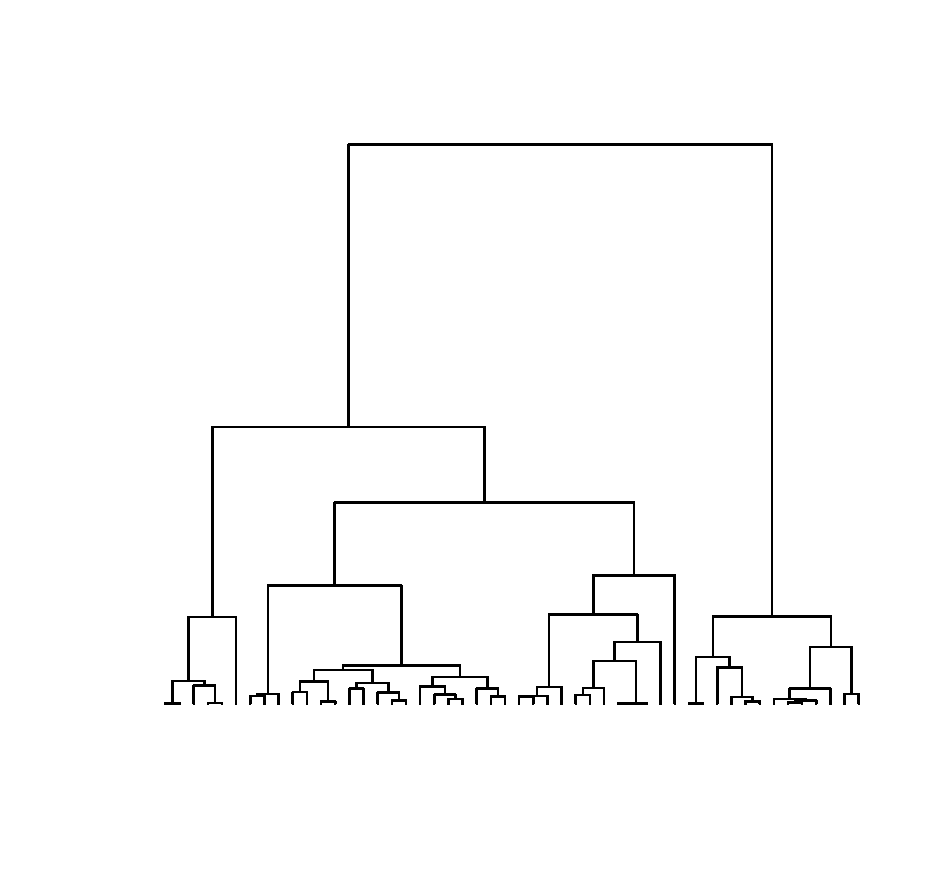
\includegraphics[width=0.6\textwidth, trim={2.8cm 3cm 1.5cm 2cm}, clip]{plots/ncoalescent.pdf}
\caption[The $n$-coalescent]{A realisation of the $n$-coalescent with $n=50$.}
\end{figure}

A particularly attractive feature of the $n$-coalescent is its tractability; its distribution and those of many statistics of interest are available in closed form (Section \ref{sec:KCproperties}).
It turns out also to be extremely useful as a limiting distribution in population genetics, including the genealogies of a wide range of population models in its domain of attraction (Section \ref{sec:popgenmodels}).


\subsection{Properties of Kingman's coalescent}\label{sec:KCproperties}
The simplicity of $Q$ allows various properties of the $n$-coalescent to be studied analytically. \seb{Refer to more exhaustive studies of the properties in the literature, e.g.\ \textcite[Section 1.2]{durrett2008}.}
Starting with $n$ blocks, exactly $n-1$ coalescences are required to reach the absorbing state where all blocks have coalesced, known in the population genetics literature as the \emph{most recent common ancestor} (MRCA).

\begin{figure}[ht]
\centering
\begin{tikzpicture}
% horizontal lines
\draw[dotted, gray] (-0.5,-1)--(6,-1);
\draw[dotted, gray] (-0.5,-0.2)--(6,-0.2);
\draw[dotted, gray] (-0.5,0.5)--(6,0.5);
\draw[dotted, gray] (-0.5,1.3)--(6,1.3);
\draw[dotted, gray] (-0.5,3.3)--(6,3.3);

% tree
\draw[thick] (0,-1)--(0,-0.2);
\draw[thick] (1,-1)--(1,-0.2);
\draw[thick] (0,-0.2)--(1,-0.2);
\draw[thick] (0.5,-0.2)--(0.5,1.3);
\draw[thick] (2,-1)--(2,1.3);
\draw[thick] (0.5,1.3)--(2,1.3);
\draw[thick] (3,-1)--(3,0.5);
\draw[thick] (4,-1)--(4,0.5);
\draw[thick] (3,0.5)--(4,0.5);
\draw[thick] (1.25,1.3)--(1.25,3.3);
\draw[thick] (3.5,0.5)--(3.5,3.3);
\draw[thick] (1.25,3.3)--(3.5,3.3);

% interval arrows
\draw[<->] (5,-1)--(5,-0.2);
\draw[<->] (5,-0.2)--(5,0.5);
\draw[<->] (5,0.5)--(5,1.3);
\draw[<->] (5,1.3)--(5,3.3);

% small t's
\node at (5.2, -0.6) {\footnotesize{$t_5$}};
\node at (5.2, 0.15) {\footnotesize{$t_4$}};
\node at (5.2, 0.9) {\footnotesize{$t_3$}};
\node at (5.2, 2.3) {\footnotesize{$t_2$}};

% capital T's
\node[anchor=west] at (6, -1) {\footnotesize{$T_5 = 0$}};
\node[anchor=west] at (6, -0.2) {\footnotesize{$T_4$}};
\node[anchor=west] at (6, 0.5) {\footnotesize{$T_3$}};
\node[anchor=west] at (6, 1.3) {\footnotesize{$T_2$}};
\node[anchor=west] at (6, 3.3) {\footnotesize{$T_1 = T_{MRCA}$}};
\end{tikzpicture}
\caption{Diagram illustrating the definitions of $t_i$, $T_i$ in the $n$-coalescent.}
\label{fig:KC_timedefns}
\end{figure}

Denote by $t_2, t_3 \dots, t_n$ the waiting times between coalescent events, where $t_i$ is the amount of time for which the coalescent has exactly $i$ distinct lineages (see Figure~\ref{fig:KC_timedefns}).
A consequence of Definition~\ref{def:kingman} is that these waiting times are independent and have distributions
\begin{equation}
t_i \sim \Exp\left( \binom{i}{2} \right) .
\end{equation}
The partial sum $T_k := \sum_{i=k+1}^n t_i$ gives the total time up to the $(n-k)^{th}$ coalescence event, i.e.\ the first time at which there are only $k$ lineages remaining out of the initial $n$ (see Figure~\ref{fig:KC_timedefns}).
The partial sums, being sums of independent Exponential random variables, have HyperExponential distributions.

\seb{Refer back to the following three properties later on with reference to their relevance in SMC.}

\subsubsection{Time to MRCA}
Of particular interest is the tree height or time to the most recent common ancestor, $T_{MRCA} := T_1$.
With some algebra we find, for instance,
\begin{equation}
\E[ T_{MRCA} ] 
= \sum_{i=2}^{n} \E[t_i]
= \sum_{i=2}^n \frac{2}{i(i-1)}
= 2 \sum_{i=2}^n \left\{ \frac{1}{i-1} - \frac{1}{i} \right\}
= 2 \left( 1 - \frac{1}{n} \right)
\end{equation}
and
\begin{equation}
\V[ T_{MRCA} ] 
= \sum_{i=2}^n \V[t_i]
= \sum_{i=2}^n \left( \frac{2}{i(i-1)} \right)^2 .
\end{equation}
The expected tree height converges to 2 as $n\to\infty$, and the variance converges to $4(\pi^2 - 9)/3 \simeq 1.16$.
The somewhat surprising fact that the tree height does not diverge with $n$ is a result of the very high rate of coalescence close to the bottom of the tree. This rate is large enough that the full Kingman coalescent (on $\mathbb{N}$) \emph{comes down from infinity}, that is, despite starting with infinitely many blocks, after any positive amount of time these have coalesced into finitely many blocks.
\seb{Plot mean with sd-ribbon over $n$ for an illustration? SD ribbon isn't the right thing; since we apparently know the actual distribution, plot a high density interval of that. (also for $L$)}


\subsubsection{Total branch length}
Another quantity of interest is the total branch length,
$ L := \sum_{i=2}^n i t_i $.
For instance
\begin{equation}
\E[ L ] 
= \sum_{i=2}^n i \E[ t_i ]
= \sum_{i=2}^n \frac{2}{i-1}
= \sum_{i=1}^{n-1} \frac{2}{i} %,
\simeq 2 \ln(n-1) 
\end{equation}
%a harmonic series, 
and
\begin{equation}
\V[ L ] 
= \sum_{i=2}^n i^2 \V[ t_i ]
= \sum_{i=2}^n \frac{4}{(i-1)^2}
= \sum_{i=1}^{n-1} \frac{4}{i^2} .
\end{equation}
Note that although the mean total branch length diverges with $n$, the variance converges to a constant, $4\pi /6 \simeq 6.6$.


\subsubsection{Probability that sample MRCA equals population MRCA}
One other interesting quantity is the probability that the MRCA of $k$ random lineages coincides with the population MRCA \parencite[e.g.][Theorem 1.7]{durrett2008}.
Denote by $S_k$ the relevant event: that a random sample of $k$ lineages has the same as the MRCA as the population.
Consider the two subtrees produced by cutting the tree just below the population MRCA. The sample of $k$ lineages coalesces before the population MRCA if and only if all $k$ sampled leaves lie in just one of these two subtrees.
A basic consequence of the exchangeability of the $n$-coalescent is that, in the limit $N\to\infty$, the proportion of leaves in the left subtree is uniformly distributed on $[0,1]$.
Calling this proportion $X$, we have
\begin{equation*}
\Prob [ S_k^c \mid X=x]
= x^k + (1-x)^k
\end{equation*}
Integrating against the distribution of $X$, the probability of interest is
\begin{equation*}
\Prob[ S_k ]
= 1- \int_0^1 [ x^k + (1-x)^k ] dx
= \frac{k-1}{k+1}
\end{equation*}
as required.

The above is based on properties of the full Kingman coalescent, but similar results are available for the $n$-coalescent.
Consider now a subsample of size $k$ among $n$ lineages that follow the $n$-coalescent.
Denote by $S_{k,n}$ the event that these $k$ lineages have the same MRCA as all $n$ lineages.
This probability of this event is calculated in \textcite[Example 1]{saunders1984} and again in \textcite[Equation (3)]{spouge2014}, in both cases arising as a special case of more general results. A direct proof is given below.

Let $X$ be the number of leaves in the left subtree. So $X \in \{1,\dots,n-1\} $ and, like before, a consequence of exchangeability is that $X$ is uniformly distributed on that set.
Now that the total number of branches is finite, we have to count more carefully. Conditional on $X$ we have
\begin{equation*}
\Prob [S_{k,n}^c \mid X=x]
= \left[ \binom{x}{k} + \binom{n-x}{k} \right] \binom{n}{k}^{-1} .
\end{equation*}
Integrating against the distribution of $X$ gives
\begin{align*}
\Prob[ S_{k,n} ]
&= 1 - \frac{1}{n-1} \binom{n}{k}^{-1} \, \sum_{x=1}^{n-1} 
        \left[ \binom{x}{k} + \binom{n-x}{k} \right] \\
&= 1 - \frac{1}{n-1} \binom{n}{k}^{-1} 
        \left[ \binom{n}{k+1} + \binom{n}{k+1} \right] \\
&= \frac{k-1}{k+1} \frac{n+1}{n-1}
\end{align*}
using binomial identities and some algebra.
As $n\to\infty$ this agrees with the population-level result above.



\subsection{Models in population genetics}\label{sec:popgenmodels}
The Kingman coalescent is the limiting coalescent process (in the large population limit) for a surprisingly wide range of population models. Some important examples of models in Kingman's ``domain of attraction'' are introduced in this section.
Common to all of these models are the following assumptions:
\begin{itemize}
\item The population has constant size $N$
\item Reproduction happens in discrete generations
\item The offspring distributions are identical at each generation, and independent between generations
\item These models are all \emph{neutral}, i.e.\ the offspring distribution is exchangeable.
\end{itemize}
As before \seb{section/eq ref?}, we define offspring counts in terms of parental indices as $\nu_j := |\{ i: a_i = j\}|$.
Under the assumption of neutrality, it is sufficient to consider only the offspring counts, rather than the parental indices (which generally carry more information).
\seb{Crucially, in the neutral case, offspring counts carry all the information about the distribution of the genealogy that is contained in the parental indices.}
From a biological perspective, neutrality encodes the absence of natural selection, i.e.\ no individual in the population is ``fitter'' than another.

\subsubsection{Wright-Fisher model}
The neutral Wright-Fisher model \parencite{fisher1923, fisher1930, wright1931} is one of the most studied models in population genetics.
At each time step the existing generation dies and is replaced by $N$ offspring. The offspring descend from parents $(a_1, \dots, a_N)$ which are selected according to
\begin{equation*}
a_i \overset{iid}{\sim} \Cat(\{1, \dots, N\}, (1/N, \dots, 1/N)).
\end{equation*}
The joint distribution of the offspring counts is therefore
\begin{equation*}
(v_1,\dots, v_N) \sim \Mn(N, (1/N, \dots, 1/N)).
\end{equation*}
Since the Multinomial distribution is exchangeable, this model is neutral.
There are several non-neutral variants of the Wright-Fisher model \seb{citations?}, but they are typically much less tractable than the neutral one.

Kingman showed in his original papers introducing the Kingman coalescent \parencite{kingman1982gene} that, when time is scaled by a factor of $N$, genealogies of the neutral Wright-Fisher model converge to the Kingman coalescent as $N\to\infty$.

\subsubsection{Cannings model}
The neutral Cannings model \parencite{cannings1974, cannings1975} is a more general construction which encompasses the neutral Wright-Fisher model as a special case.

In the Cannings model, the particular offspring distribution is not specified; we only require that it is exchangeable, i.i.d.\ between generations, and preserves the population size. In particular, the probability of observing offspring counts $(v_1, \dots, v_N)$ must be invariant under permutations of this vector.

Genealogies of the neutral Cannings model also converge to the Kingman coalescent, under some conditions and a suitable time-scaling \seb{which is what?}, as $N\to\infty$ \parencite[see for example][Section 2.2]{etheridge2011}. \seb{original reference for this? is not any Kingman 1982 papers, and certainly not Cannings 1974/5 which predates KC}

\subsubsection{Moran model}
The neutral Moran model \parencite{moran1958}, while perhaps less biologically relevant, is mathematically appealing because its simple dynamics make it particularly tractable.

At each time step, an ordered pair of individuals is selected uniformly at random. The first individual in this pair dies (i.e.\ leaves no offspring in the next generation), while the other reproduces (leaving two offspring). All of the other individuals leave exactly one offspring.
%Usually the model is thought of as having ``overlapping generations'': the individuals having one offspring are considered to be not reproducing but rather surviving to appear again in the next generation.
%However, one can equally think of it as having non-overlapping generations and a low variance reproduction mechanism.
This is another special case of the neutral Cannings model, where the offspring distribution is now uniform over all permutations of $(0,2,1,1,\dots,1)$.
Therefore we know that under a suitable time-scaling, its genealogies converge to the Kingman coalescent. The time scale in this case is $N^2$, because reproduction happens at a rate $N$ times \seb{or is it technically N-1 times?} lower than in the Wright-Fisher model. \seb{also cite a Moran-specific convergence result: not sure where (it isn't in Kingman 1982* or in Moran 1958 which predates KC)}


\subsection{Particle populations}
Much of the population genetics framework transfers readily to the case of SMC. The population is now a population of particles, with each iteration of the SMC algorithm corresponding to a generation, and resampling playing the part of reproduction.
In fact, SMC ``populations'' are in some ways more suited to these population models than actual populations of organisms.
The assumptions that the population has constant size $N$ and that reproduction occurs only at discrete generations are satisfied by construction.
However, we cannot assume independence between generations: as seen in Figure~\ref{fig:cond_indep_graph}, the offspring counts at subsequent generations are not independent without some conditioning. In fact, after marginalising out the information about the positions of the particles, the genealogical process is not even Markovian.
Nor is our model neutral: the resampling distribution depends on the weight of each particle (the weight plays the role of fitness in a non-neutral population model).






\section{Sequential Monte Carlo genealogies}

\subsection{From particles to genealogies}
\draft{How does the SMC algorithm induce a genealogy? (resampling = parent-child relationship).}

\subsection{Performance}
\draft{How do genealogies affect performance? Variance (and variance estimation?), storage cost. Ancestral degeneracy.}

\begin{figure}[ht]
\centering
\subfloat[Multinomial resampling]{
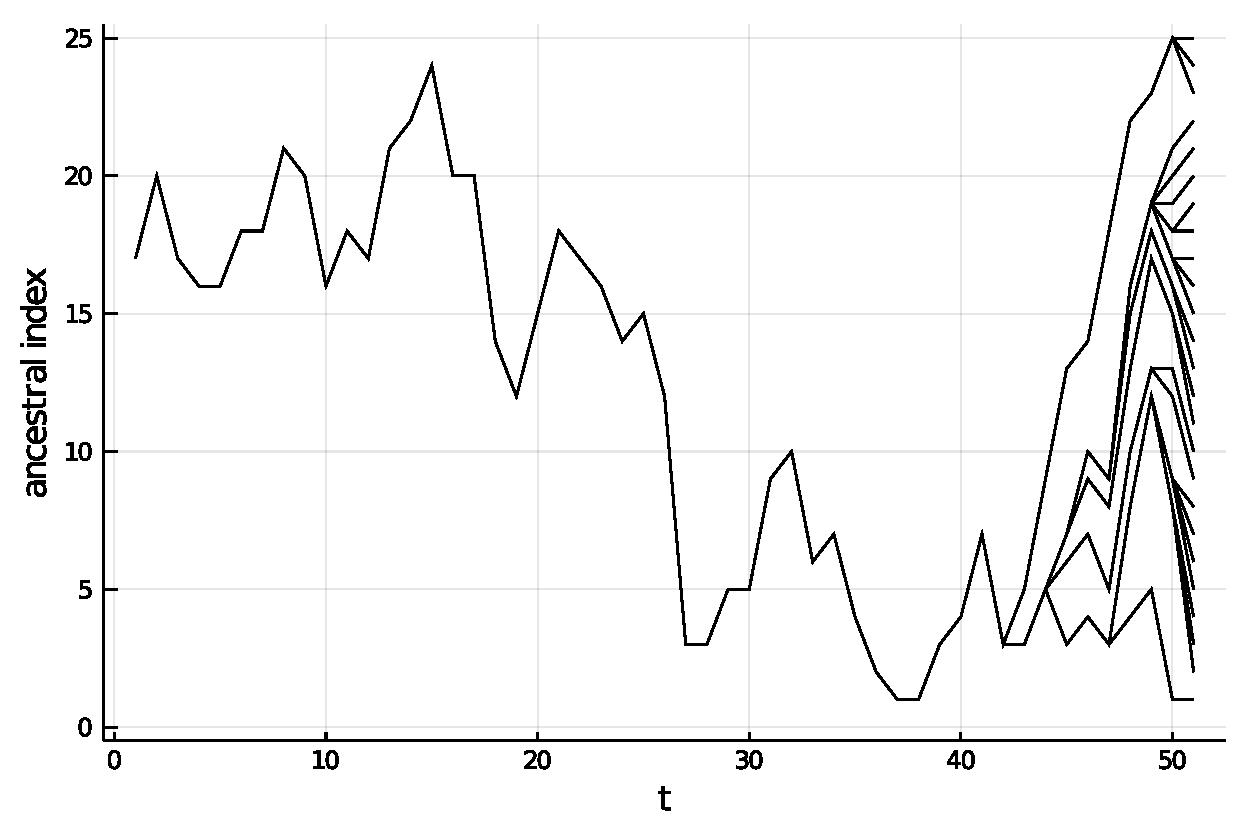
\includegraphics[width=0.5\textwidth]{plots/ancdegen_mn.pdf}
\label{fig:ancdegen_mn}
}
\subfloat[Adaptive minimum-variance resampling]{
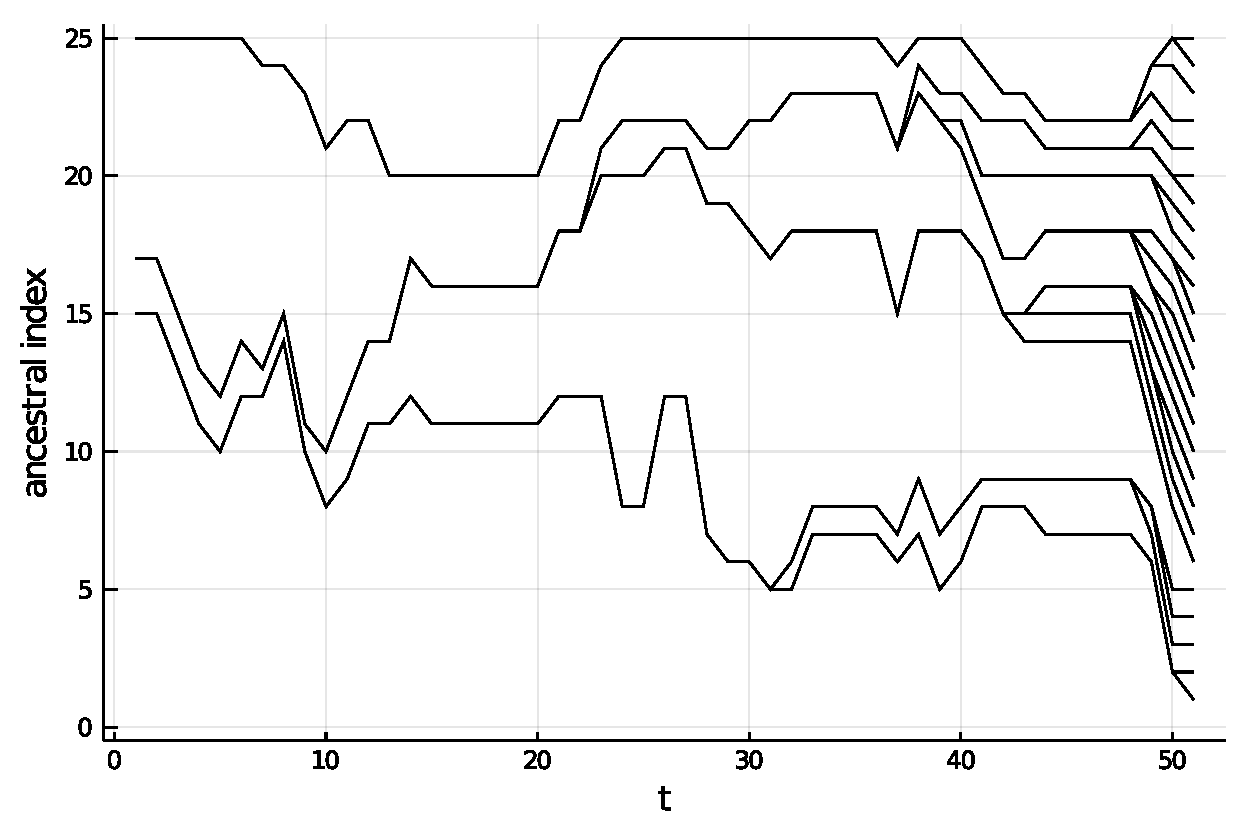
\includegraphics[width=0.5\textwidth]{plots/ancdegen_adaptsyst.pdf}
\label{fig:ancdegen_adaptsyst}
}
\caption[Ancestral degeneracy illustration]{Illustration of ancestral degeneracy and the mitigating effect of low-variance and adpative resampling. \subref{fig:ancdegen_mn} with multinomial resampling, \subref{fig:ancdegen_adaptsyst} the same system with adaptive systematic resampling.}
\label{fig:ancestral_degeneracy}
\end{figure}

\subsection{Mitigating ancestral degeneracy}
\draft{Low-variance resampling (save details for next section). Adaptive resampling: idea of balancing weight/ancestral degeneracy; rule of thumb for implementing it; when is it effective or not?; necessary changes to our generic SMC algorithm (calculation of weights in particular). Backward sampling: when is it possible to do this?}

\subsection{Asymptotics}
\draft{Why are large population asymptotics useful? Existing results (path storage, KJJS).}



\section{Resampling \seb{$\sim$} }
As we have seen, resampling is necessary within SMC to ``reset'' the weights in order to prevent weight degeneracy.
The basic role of a resampling scheme is to map the continuous weights to discrete offspring counts, in some ``sensible'' way (Definition~\ref{defn:resampling}).
The choice of resampling scheme is explored in detail in this section.
%There are other considerations when choosing between the many possible resampling schemes; some of these are explored in Section~\ref{sec:resampling_properties}, and some popular choices of resampling scheme are described in Section~\ref{sec:examples_resamplingschemes}.

\subsection{Definition \seb{$\checkmark$} }
\draft{Also say that resampling is itself a Monte Carlo procedure.}

\begin{defn}\label{defn:resampling}
For our purposes, a valid resampling scheme is a stochastic function mapping weights 
$w_t^{(1:N)} \in \mathcal{S}_{N-1}$ 
to offspring counts 
$\nu_t^{(1:N)} \in \{0,\dots,N\}^N $
that satisfies the following properties:
\begin{enumerate}
\item\label{item:resampling_property1} the population size is conserved:
$ \sum_{i=1}^N \nu_t^{(i)} =N $ for all $N$
\item\label{item:resampling_property2} the weights are uniform after resampling:
$w_{t+}^{(i)} = 1/N$ for all $i$
\item\label{item:resampling_property3} the resampling is unbiased:
$ \E[ \nu_t^{(i)} \mid w_t^{(i)} ] = N w_t^{(i)} $ for all $i$.
\end{enumerate}
\end{defn}
It is possible to design resampling schemes that violate these properties.
For example, a scheme of \textcite{liu1998} uses the square roots of the weights for resampling, then corrects by setting non-uniform weights after resampling (violating conditions \ref{item:resampling_property2} and \ref{item:resampling_property3}).
\seb{\textcite[p.890, point (d)]{fearnhead2003} also appears to resample such that the weights are not uniform after resampling.}
%
Resampling different numbers of particles in different iterations (violating condition \ref{item:resampling_property1}) is of course possible, but we typically have a fixed limit on computational resources, in which case it makes sense to simulate the maximum feasible number of particles $N$ at every iteration.
%
Deterministic resampling schemes (which cannot generally be unbiased, violating condition \ref{item:resampling_property3}) have been used by some authors. These include schemes based on optimal transport \parencite{reich2013, myers2021, corenflos2021} and the importance support points resampling of \textcite{huang2020}.
However, the majority of resampling schemes in the literature fit within Definition~\ref{defn:resampling}, and it is not typically advantageous to violate the properties \ref{item:resampling_property1}--\ref{item:resampling_property3}.

Within Definition~\ref{defn:resampling} there is still a great deal of flexibility. Many different resampling schemes have been proposed in the literature, some of which perform better than others.
 Section~\ref{sec:examples_resamplingschemes} introduces some important resampling schemes, and their properties are discussed in Section~\ref{sec:resampling_properties}. 
These are summarised in Table~\ref{tab:resampling_properties}.



\subsection{Examples \seb{$\sim$} }\label{sec:examples_resamplingschemes}
\draft{Argue in each case that the scheme is unbiased.}

\begin{table}[ht]
\centering
\begin{tabular}{ l l }
\hline\hline
Abbreviation & Description \\% & Defined in Section \\
\hline
\texttt{multi} & multinomial resampling \\%& \ref{sec:resampling_multinomial} \\
\texttt{star} & star resampling \\%& \ref{sec:resampling_star} \\
\texttt{strat} & stratified resampling \\%& \ref{sec:resampling_stratified} \\
\texttt{syst} & systematic resampling \\%& \ref{sec:resampling_systematic} \\
\texttt{res-multi} & residual resampling with multinomial residuals \\
        %& \ref{sec:resampling_residual} \\
\texttt{res-star} & residual resampling with star residuals \\
        %& \ref{sec:resampling_residual} \\
\texttt{res-strat} & residual resampling with stratified residuals \\
        %& \ref{sec:resampling_residual} \\
\texttt{res-syst} & residual resampling with systematic residuals \\
        %& \ref{sec:resampling_residual} \\
\texttt{ssp} & Srinivasan sampling procedure resampling \\%& \\
\texttt{branch} & minimal variance branching algorithm \\%& \\
\hline\hline
\end{tabular}
\caption{Abbreviations for resampling schemes}
\label{tab:resampling_abbrevs}
\end{table} 


 
\subsubsection{Multinomial resampling \seb{$\checkmark$} }%\label{sec:resampling_multinomial}
Multinomial resampling \parencite{gordon1993,efron1994} is one of the simplest resampling schemes.
The parental indices are chosen independently from $\{1, \dots, N\}$, each with probability given by the weight of the corresponding particle $w_t^{(i)}$. 
That is, 
\begin{equation*}
a_t^{(1:N)} \sim \Cat( \{1,\dots, N\}, w_t^{(1:N)} ) .
\end{equation*}
This implies the joint distribution of the offspring counts is 
\begin{equation*}
\nu_t^{(1:N)} \eqdist \operatorname{Multinomial}(N, w_t^{(1:N)} ) .
\end{equation*}
It follows from the mean of the Multinomial distribution that this resampling scheme is unbiased.
\seb{Although the parental indices are chosen independently, the resulting offspring counts are negatively correlated. --- link to GCW19's negative association?}

A simple way to sample the parental indices is to use inversion sampling: partition the unit interval into $N$ subintervals each of which will correspond to a certain index $i$ and has length equal to the weight $w_t^{(i)}$; then draw $N$ samples $U_i \sim \Unif(0,1)$ and classify them according to which of these subintervals they fall in.
Explicitly, the parental index assigned to child $i$ is the index $a_i$ satisfying
\begin{equation}\label{eq:syst_strat_resampling}
\sum_{j=1}^{a_i -1} w_t^{(j)} \leq U_i \leq \sum_{j=1}^{a_i} w_t^{(j)} .
\end{equation}
This is illustrated in Figure \ref{fig:resampling_mn}. 
%Note that there exist more efficient methods to sample from a Multinomial distribution, so the inversion method may not be used in practice.

Fast implementations of multinomial resampling rely on $U_1,\dots,U_N$ being pre-sorted, which speeds up the search step \eqref{eq:syst_strat_resampling}. Sorting $N$ numbers is an $O(N\log N)$ operation, but in fact this is not necessary because we can directly sample the order statistics of a $\Unif[0,1]$ distribution \seb{[citations: \textcite{chopin2020}, and a different (or possibly equivalent) method in \textcite{hol2006}] ---explore whether these methods are equivalent}.
This allows multinomial resampling to be implemented at $O(N)$ cost, with the side-effect that the sampled ancestral indices will be ordered. \seb{And therefore the sampled parental indices cannot be Cat(N,w) distributed. But the counts are still Multinomial? And anyway for the purposes of resampling this isn't a problem; it might even improve performance?}


\subsubsection{Residual resampling \seb{$\checkmark$} }%\label{sec:resampling_residual}
Residual resampling is described in \textcite{liu1998} and also in \textcite{whitley1994} where it is called ``remainder stochastic sampling''.

Each particle $X_{t}^{(i)}$ is deterministically assigned $\flnw$ offspring and the remaining $R := \sum_{i=1}^N ( Nw_t^{(i)} - \flnw) = n                           N- \sum_{i=1}^N \flnw$ offspring are assigned stochastically according to the residual weights
\begin{equation*}
r^{(i)} := ( Nw_t^{(i)} - \flnw) /R .
\end{equation*}
Notice that each $r^{(i)}$ lies in the interval $(0, 1/R)$.

The stochastic part can be done using any of the other basic resampling schemes (e.g.\ multinomial, stratified, systematic). Most presentations focus on the case where multinomial resampling is used for the residuals, which is by no means the most sensible option. We will explore several different options in what follows.

%This yields a vector of offspring counts
%\begin{equation*}
%\nu_t^{(1:N)} \eqdist \lfloor N w_t^{(1:N)} \rfloor +  \operatorname{Multinomial}(R, (N w_t^{(1:N)} - \lfloor N w_t^{(1:N)}\rfloor)/R) .
%\end{equation*}
%The deterministic part ensures that every particle with weight $>1/N$ is guaranteed to survive. This is a desirable property as it prevents the random loss of high-weighted particles.



\begin{figure}
\centering
\subfloat[Multinomial resampling]{
\begin{tikzpicture}
%parallel lines
\draw[thick] (0,0) -- (12,0);
\draw (0,2) -- (12,2);
% tick marks at ends
\draw[thick] (0,0.1) --(0,-0.1);
\draw[thick] (12,0.1) --(12,-0.1);
\draw (0,2.1) --(0,1.9);
\draw (12,2.1) --(12,1.9);
% tick marks indicating weights
\draw[thick] (3,0.1) --(3,-0.1);
\draw[thick] (5,0.1) --(5,-0.1);
\draw[thick] (11,0.1) --(11,-0.1);
% weight labels
\node at (1.5,-0.3) {$w_1$};
\node at (4,-0.3) {$w_2$};
\node at (8,-0.3) {$w_3$};
\node at (11.5,-0.3) {$w_4$};
% endpoint labels
\node at (-0.2,2) {$0$};
\node at (12.2,2) {$1$};
% uniform points
\filldraw[violet] (10.94,2) circle (2pt);
\filldraw[violet] (1.06,2) circle (2pt);
\filldraw[violet] (8.82,2) circle (2pt);
\filldraw[violet] (3.16,2) circle (2pt);
% arrows from random points
\draw[thick, violet, ->] (10.94,2) -- (10.94,0);
\draw[thick, violet, ->] (1.06,2) -- (1.06,0);
\draw[thick, violet, ->] (8.82,2) -- (8.82,0);
\draw[thick, violet, ->] (3.16,2) -- (3.16,0);
\end{tikzpicture}
\label{fig:resampling_mn}
}\\
\subfloat[Stratified resampling]{
\begin{tikzpicture}
%parallel lines
\draw[thick] (0,0) -- (12,0);
\draw (0,2) -- (12,2);
% tick marks at ends
\draw[thick] (0,0.1) --(0,-0.1);
\draw[thick] (12,0.1) --(12,-0.1);
\draw (0,2.1) --(0,1.9);
\draw (12,2.1) --(12,1.9);
% tick marks indicating weights
\draw[thick] (3,0.1) --(3,-0.1);
\draw[thick] (5,0.1) --(5,-0.1);
\draw[thick] (11,0.1) --(11,-0.1);
% tick marks indicating sampling intervals:
\draw (3,2.1) --(3,1.9);
\draw (6,2.1) --(6,1.9);
\draw (9,2.1) --(9,1.9);
% weight labels
\node at (1.5,-0.3) {$w_1$};
\node at (4,-0.3) {$w_2$};
\node at (8,-0.3) {$w_3$};
\node at (11.5,-0.3) {$w_4$};
% endpoint labels
\node at (-0.2,2) {$0$};
\node at (12.2,2) {$1$};
% stratified points
\filldraw[violet] (2.735,2) circle (2pt);
\filldraw[violet] (3.265,2) circle (2pt);
\filldraw[violet] (8.205,2) circle (2pt);
\filldraw[violet] (9.79,2) circle (2pt);
% arrows from random points
\draw[thick, violet, ->] (2.735,2) -- (2.735,0);
\draw[thick, violet, ->] (3.265,2) -- (3.265,0);
\draw[thick, violet, ->] (8.205,2) -- (8.205,0);
\draw[thick, violet, ->] (9.79,2) -- (9.79,0);
\end{tikzpicture}
\label{fig:resampling_stratified}
}\\
\subfloat[Systematic resampling]{
\begin{tikzpicture}
%parallel lines
\draw[thick] (0,0) -- (12,0);
\draw (0,2) -- (12,2);
% tick marks at ends
\draw[thick] (0,0.1) --(0,-0.1);
\draw[thick] (12,0.1) --(12,-0.1);
\draw (0,2.1) --(0,1.9);
\draw (12,2.1) --(12,1.9);
% tick marks indicating weights
\draw[thick] (3,0.1) --(3,-0.1);
\draw[thick] (5,0.1) --(5,-0.1);
\draw[thick] (11,0.1) --(11,-0.1);
% tick marks indicating sampling intervals:
\draw (3,2.1) --(3,1.9);
\draw (6,2.1) --(6,1.9);
\draw (9,2.1) --(9,1.9);
% weight labels
\node at (1.5,-0.3) {$w_1$};
\node at (4,-0.3) {$w_2$};
\node at (8,-0.3) {$w_3$};
\node at (11.5,-0.3) {$w_4$};
% endpoint labels
\node at (-0.2,2) {$0$};
\node at (12.2,2) {$1$};
% stratified points
\filldraw[violet] (2.735,2) circle (2pt);
\filldraw[violet] (5.735,2) circle (2pt);
\filldraw[violet] (8.735,2) circle (2pt);
\filldraw[violet] (11.735,2) circle (2pt);
% arrows from random points
\draw[thick, violet, ->] (2.735,2) -- (2.735,0);
\draw[thick, violet, ->] (5.735,2) -- (5.735,0);
\draw[thick, violet, ->] (8.735,2) -- (8.735,0);
\draw[thick, violet, ->] (11.735,2) -- (11.735,0);
\end{tikzpicture}
\label{fig:resampling_systematic}
}\\
\caption[Resampling using multinomial, stratified and systematic schemes]{Inversion sampling to obtain Multinomial offspring counts, where the (marginally) Uniform variables for inversion are sampled in different ways. For this example $N=4$ and the weights are $w_{(1:4)} = \frac{1}{N}(1,\frac{2}{3},2,\frac{1}{3})$. 
\seb{Also make the same diagram in Whitley's ``roulette wheel'' style, to illustrate the difference. Or maybe make it for the ``degeneracy under equal weights'' section just illustrating the difference it makes in stratified resampling.}
%In each case the samples to be inverted are seeded with the same $\Unif(0,1)$ samples.
%\subref{fig:resampling_mn} Sample $N$  independent $\Unif(0,1)$ random variables. In this example the sampled offspring counts are $(1,1,2,0)$.
%\subref{fig:resampling_stratified} The $\Unif(0,1)$ samples are transformed to Uniform draws from the intervals (0,0.25), (0.25,0.5), (0.5, 0.75), (0.75,1). In this example the sampled offspring counts are $(1,1,2,0)$.
%\subref{fig:resampling_systematic} Use only the first draw and transform it to a sample from $\Unif(0,0.25)$. For the subsequent samples, add 0.25 each time to obtain a sample in each interval. In this example the sampled offspring counts are $(1,0,2,1)$.
}
\end{figure}



\subsubsection{Stratified resampling \seb{$\checkmark$} }%\label{sec:resampling_stratified}
Stratified resampling is introduced in \cite{kitagawa1996}.

As in multinomial resampling, stratified resampling uses inversion sampling to dample the parental indices. However, the samples used for inversion sampling are no longer i.i.d. $\Unif[0,1]$ samples. Instead, one number is sampled from each subinterval of length $1/N$; that is, 
\begin{equation*}
U_i \sim \Unif \left(\frac{i-1}{N}, \frac{i}{N} \right) .
\end{equation*}
Alternatively, one may think of standard Uniform samples $u_1,\dots,u_N \sim^{iid} \Unif[0,1]$ with the transformation
\begin{equation*}
U_i = \frac{u_i + i -1}{N}
\end{equation*}
to give the stratified samples $U_1,\dots,U_N$.

The parents are then assigned as in \eqref{eq:syst_strat_resampling}.
This is illustrated in Figure \ref{fig:resampling_stratified}.
The offspring distribution is no longer Multinomial, since parental indices are not chosen independently.
This scheme ensures that the samples are ``well spread out'', which reduces the probability of randomly losing high-weight particles or duplicating low-weight particles.

It will be useful later on to have a better idea about the marginal distributions of $\nu_t^{(i)}$ that are induced by stratified resampling. There are complex dependencies between the offspring counts, but we can still find some constraints on the distribution of each count conditional on the corresponding weight.
Write the $i^{th}$ weight in the form $w_t^{(i)} = (k + \delta)/N$, where $\delta \in [0,1)$ and $k\in \{0,\dots,N-1\}$.
Considering the illustration Figure~\ref{fig:resampling_stratified}, the distribution of $\nu_t^{(i)}$ depends not only on $w_t^{(i)}$ but also on where the $i^{th}$ weight interval falls with respect to the length-$(1/N)$ intervals. There are two cases to consider, which are illustrated in Figure~\ref{fig:strat_cases}. Note that Case \subref{fig:strat_case2} cannot happen if $k=0$.

%\begin{figure}
%\centering
%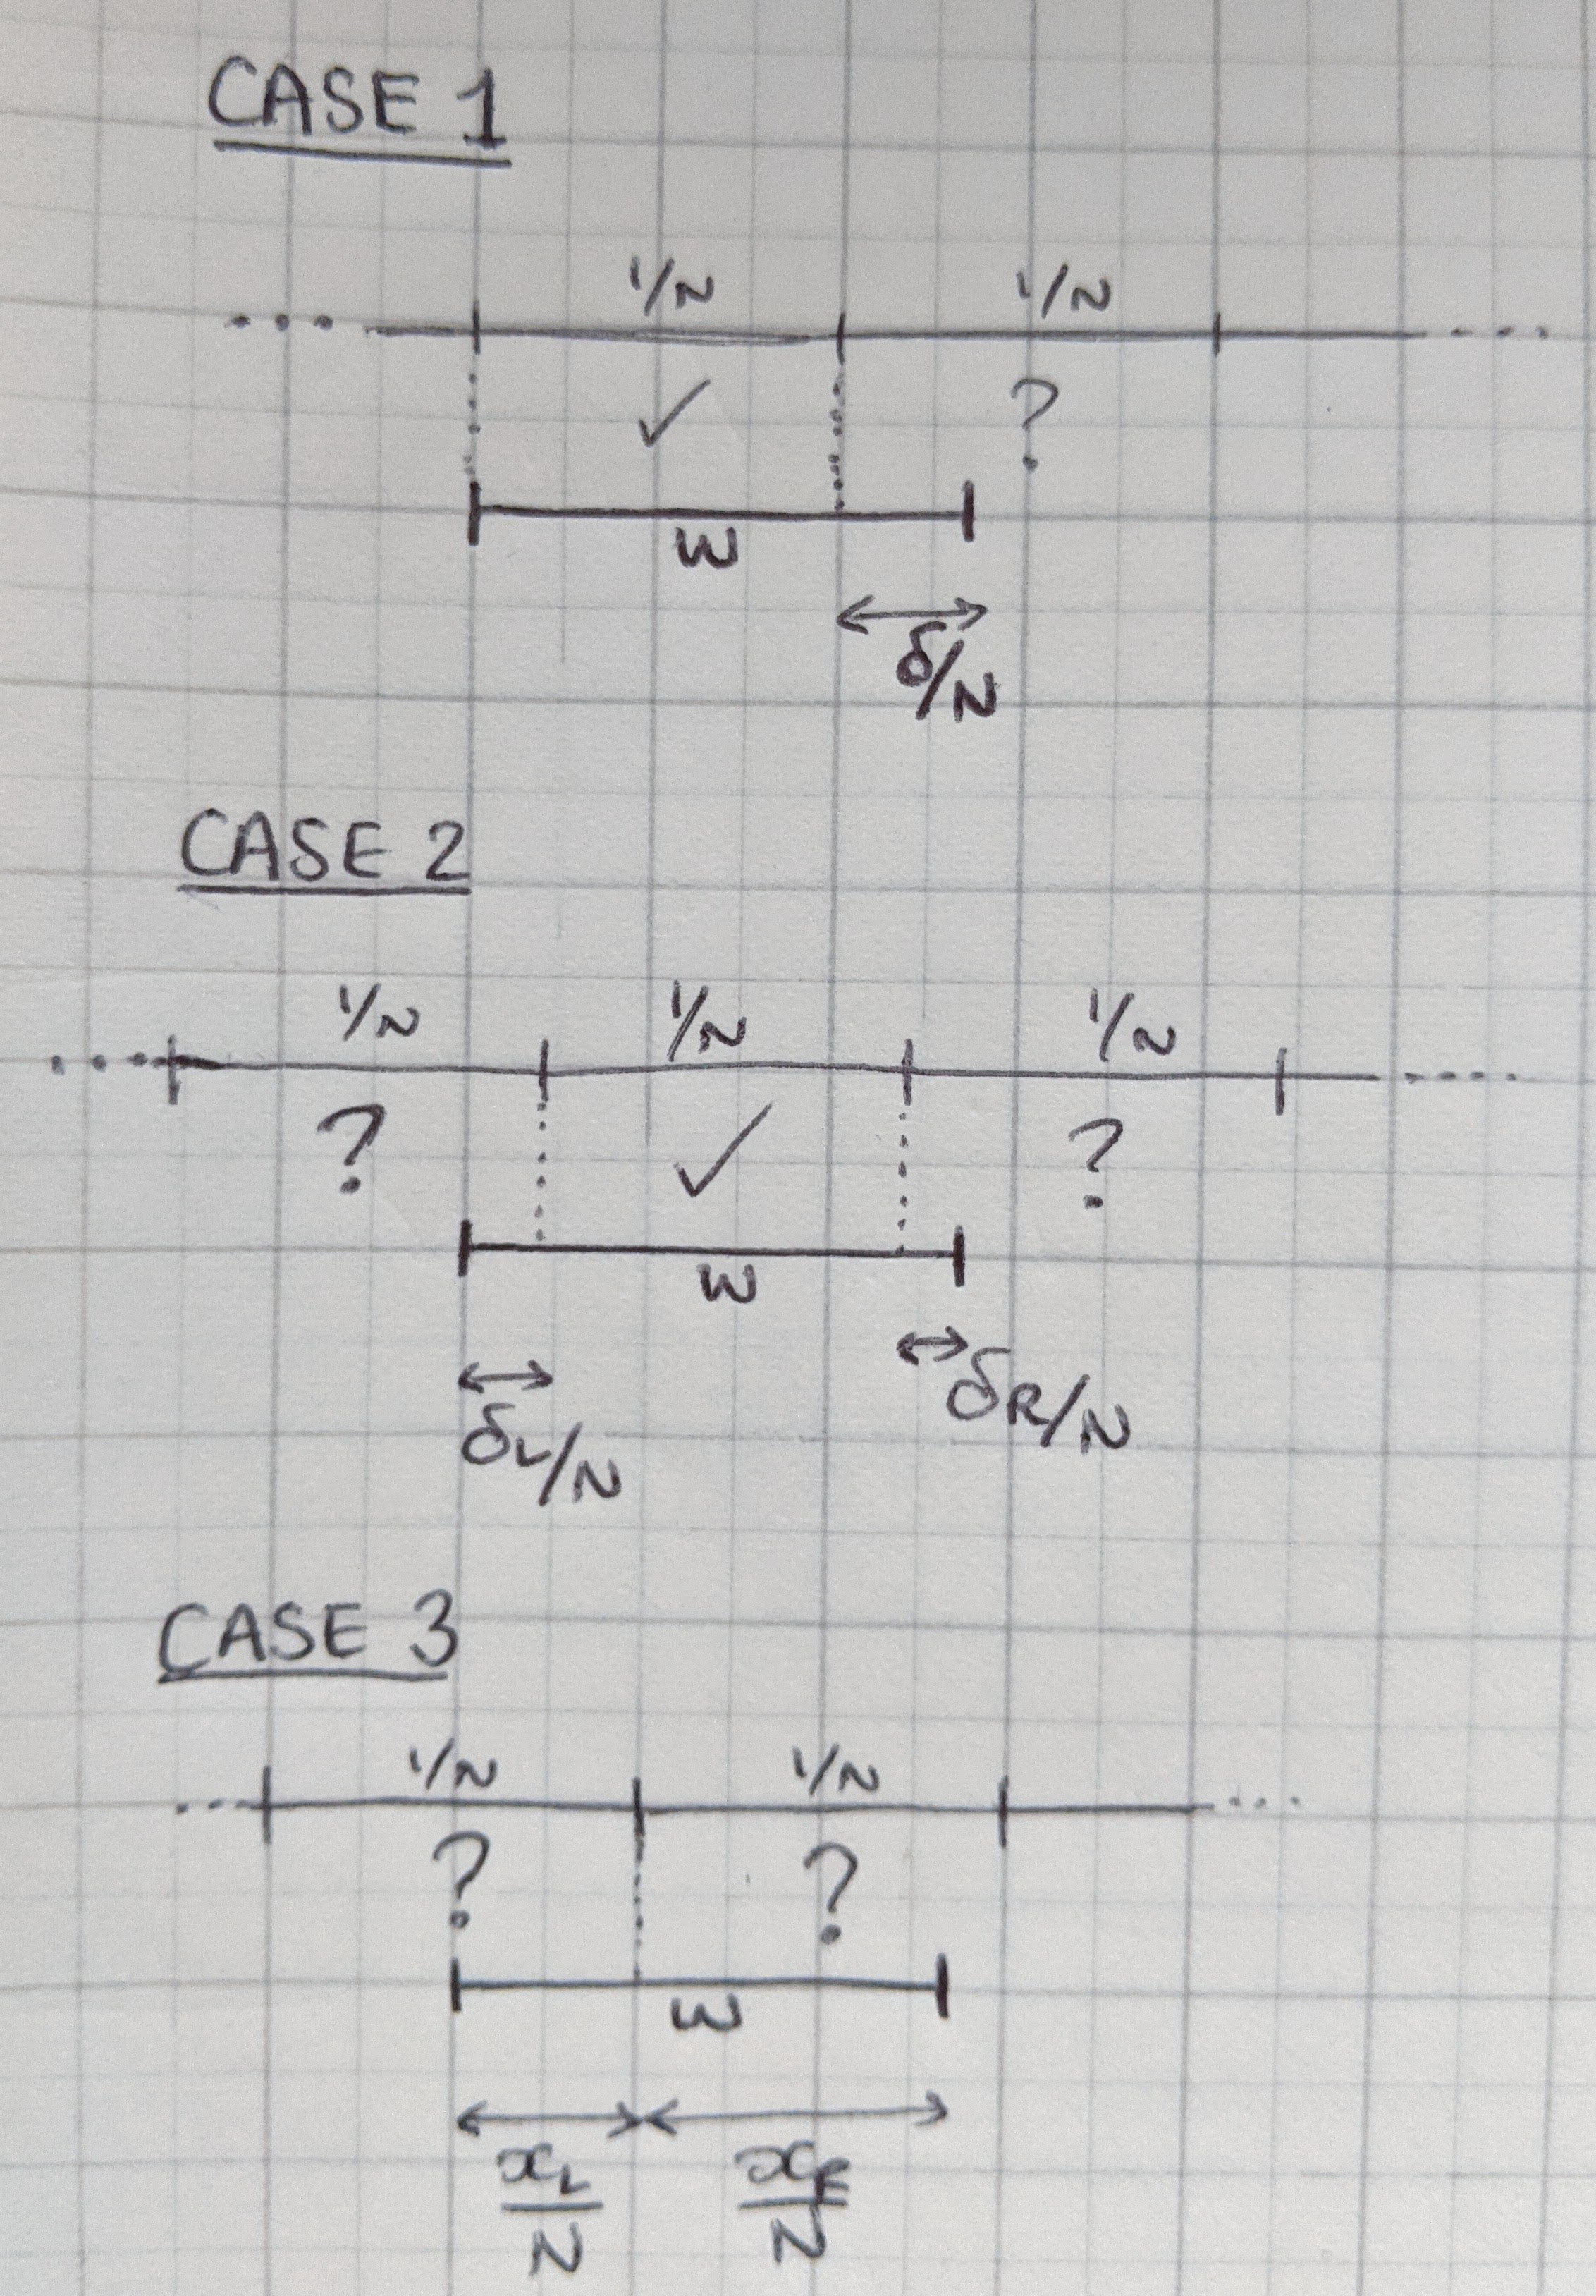
\includegraphics[width=0.4\textwidth]{plots/cases_sketch.jpg}
%\caption[PLACEHOLDER Cases for stratified resampling with a fixed weight]{PLACEHOLDER Cases for stratified resampling with a fixed weight. When I make this properly I need to allow for general $k$ rather than fixing $k=1$ as done here. Case 3 is only valid for $k\geq1$.}
%\label{fig:strat_cases_temp}
%\end{figure}

\begin{figure}
\centering
%\subfloat[Case 1]{
%\begin{tikzpicture}
%% w subinterval
%\draw[thick] (0,0)--(1.9,0);
%\draw[thick,dotted] (1.9,0)--(2.3,0);
%\draw[thick] (2.3,0)--(4.8,0);
%\draw[thick] (0,0.1)--(0,-0.1);
%\draw[thick] (4.8,0.1)--(4.8,-0.1);
%\node[anchor=north] at (2.4,0) {$w$};
%% length labels
%\draw[<->] (0,-0.4)--(4,-0.4);
%\node[anchor=north] at (2,-0.4) {$k/N$};
%\draw[<->] (4,-0.4)--(4.8,-0.4);
%\node[anchor=north] at (4.4,-0.4) {$\delta/N$};
%% sampling interval
%\draw (-0.5,1.5)--(8.5,1.5);
%\draw[dotted] (-1,1.5)--(-0.5,1.5);
%\draw[dotted] (8.5,1.5)--(9,1.5);
%\draw (0,1.6)--(0,1.4);
%\draw (4,1.6)--(4,1.4);
%\draw (8,1.6)--(8,1.4);
%\node[anchor=south] at (2,1.5) {$k/N$};
%\node[anchor=south] at (6,1.5) {$1/N$};
%% vertical dividers
%\draw[dashed, gray] (0,1.4)--(0,0.1);
%\draw[dashed, gray] (4,1.4)--(4,0.1);
%\end{tikzpicture}
%}\\
\subfloat[The parent under consideration is automatically assigned $k$ offspring, plus up to two more. ($\delta_L+\delta_R=\delta$.) ]{ %\delta_L, \delta_R \in [0,\delta]. 
\begin{tikzpicture}
% w subinterval
\draw[thick] (0,0)--(1.9,0);
\draw[thick,dotted] (1.9,0)--(2.3,0);
\draw[thick] (2.3,0)--(4.8,0);
\draw[thick] (0,0.1)--(0,-0.1);
\draw[thick] (4.8,0.1)--(4.8,-0.1);
\node[anchor=north] at (2.4,0) {$w$};
% length labels
\draw[<->] (0.3,-0.4)--(4.3,-0.4);
\node[anchor=north] at (2,-0.4) {$k/N$};
\draw[<->] (4.3,-0.4)--(4.8,-0.4);
\node[anchor=north] at (4.55,-0.4) {$\delta_R/N$};
\draw[<->] (0,-0.4)--(0.3,-0.4);
\node[anchor=north] at (0.15,-0.4) {$\delta_L/N$};
% sampling interval
\draw (-4.2,1.5)--(8.8,1.5);
\draw[dotted] (-4.7,1.5)--(-4.2,1.5);
\draw[dotted] (8.8,1.5)--(9.3,1.5);
\draw (-3.7,1.6)--(-3.7,1.4);
\draw (0.3,1.6)--(0.3,1.4);
\draw (4.3,1.6)--(4.3,1.4);
\draw (8.3,1.6)--(8.3,1.4);
\node[anchor=south] at (-1.7,1.5) {$1/N$};
\node[anchor=south] at (2.3,1.5) {$k/N$};
\node[anchor=south] at (6.3,1.5) {$1/N$};
% vertical dividers
\draw[dashed, gray] (0.3,1.4)--(0.3,0.1);
\draw[dashed, gray] (4.3,1.4)--(4.3,0.1);
\end{tikzpicture}
\label{fig:strat_case1}
}\\
\subfloat[This case can only occur when $k\geq1$. The parent under consideration is automatically assigned $k-1$ offspring, plus up to two more. ($x_L+x_R=1+\delta$.)]{ %$x_L,x_R \in [\delta,1] $. 
\begin{tikzpicture}
% w subinterval
\draw[thick] (-2,0)--(1.9,0);
\draw[thick,dotted] (1.9,0)--(2.3,0);
\draw[thick] (2.3,0)--(6.8,0);
\draw[thick] (-2,0.1)--(-2,-0.1);
\draw[thick] (6.8,0.1)--(6.8,-0.1);
\node[anchor=north] at (2.4,0) {$w$};
% length labels
\draw[<->] (0.3,-0.4)--(4.3,-0.4);
\node[anchor=north] at (2,-0.4) {$(k-1)/N$};
\draw[<->] (4.3,-0.4)--(6.8,-0.4);
\node[anchor=north] at (5.55,-0.4) {$x_R/N$};
\draw[<->] (-2,-0.4)--(0.3,-0.4);
\node[anchor=north] at (-1.15,-0.4) {$x_L/N$};
% sampling interval
\draw (-4.2,1.5)--(8.8,1.5);
\draw[dotted] (-4.7,1.5)--(-4.2,1.5);
\draw[dotted] (8.8,1.5)--(9.3,1.5);
\draw (-3.7,1.6)--(-3.7,1.4);
\draw (0.3,1.6)--(0.3,1.4);
\draw (4.3,1.6)--(4.3,1.4);
\draw (8.3,1.6)--(8.3,1.4);
\node[anchor=south] at (-1.7,1.5) {$1/N$};
\node[anchor=south] at (2.3,1.5) {$(k-1)/N$};
\node[anchor=south] at (6.3,1.5) {$1/N$};
% vertical dividers
\draw[dashed, gray] (0.3,1.4)--(0.3,0.1);
\draw[dashed, gray] (4.3,1.4)--(4.3,0.1);
\end{tikzpicture}
\label{fig:strat_case2}
}
\caption[Cases for stratified resampling with a fixed weight]{Cases for stratified resampling with a fixed weight $w = (k+\delta)/N$}
\label{fig:strat_cases}
\end{figure}


In any case $\nu_t^{(i)} \in \{k-1,k,k+1,k+2\}$ almost surely. 
To define a probability distribution over these four values, we introduce the notation $p_j := \Prob[ \nu_t^{(i)} = \flnw +j \mid w_t^{(i)} ]$, for $j=-1,0,1,2$. 
Since the sample within each interval of length $1/N$ is uniform over that interval, we find the probabilities given in Table~\ref{tab:strat_probs}, in terms of $\delta$ and the other quantities $\delta_L, \delta_R \in [0, \delta]$ and $x_L, x_R \in [\delta,1]$ defined in Figure~\ref{fig:strat_cases}. The probabilities do not depend on $k$, but of course the corresponding values of $\nu_t^{(i)}$ do. By definition $\delta_L+\delta_R=\delta$ and $x_L+x_R=1+\delta$.

\begin{table}[ht]
\centering
\begin{tabular}{ c | c c c c }
\hline\hline
& Case \subref{fig:strat_case1} & Case \subref{fig:strat_case2} & L.B. & U.B. \\
\hline
$p_{-1}$ & 0 & $x_Lx_R-\delta$ & 0 & $(1-\delta)^2 /4$ \\
$p_0$ & $1-\delta + \delta_L\delta_R$ & $1+\delta-2x_Lx_R$ & $(1-\delta)^2 /2$ 
        & $1 - 3\delta /4$ \\
$p_1$ & $\delta-2\delta_L\delta_R$ & $x_Lx_R$ & $\delta /2$ & $(1+\delta)/2$ \\
$p_2$ & $\delta_L\delta_R$ & 0 & 0 & $\delta^2 /4$ \\
\hline\hline
\end{tabular}
\caption[Analysis of distribution of offspring counts under stratified resampling]{Marginal probability distribution of $\nu_t^{(i)}$ conditional on $w_t^{(i)}$, in terms of $\delta$ and the quantities defined in Figure~\ref{fig:strat_cases}, along with upper and lower bounds on these in terms of $\delta$ only.}
\label{tab:strat_probs}
\end{table}

%By considering the constraints on $\delta_L, \delta_R, x_L, x_R$, we also have the following properties which hold in every case (i.e.\ for any $w_t^{(i)}$):
%\begin{itemize}
%\item $p_{-1} \leq 1/4$
%\item $p_{2} \leq 1/4$
%\item only one of $p_{-1}, p_2$ can be non-zero.
%\end{itemize}




\subsubsection{Systematic resampling \seb{$\checkmark$} }%\label{sec:resampling_systematic}
Systematic resampling is described in \textcite{carpenter1999} and also in \textcite{whitley1994} where it is called ``stochastic universal sampling''.

Like stratified resampling, it uses the inversion sampler of multinomial resampling but starts with a more regular set of points in $[0,1]$.
In this scheme, only one standard Uniform sample is drawn, $u \sim \Unif[0,1]$, from which the $N$ samples are generated by via the transformation
\begin{equation*}
U_i = \frac{u+ i-1}{N}
\end{equation*}
for $i = 1, \dots, N $.
The parental indices are again selected according to \eqref{eq:syst_strat_resampling}. 
The method is illustrated in Figure \ref{fig:resampling_systematic}.

\textcite{kitagawa1996} suggests a deterministic scheme in which the random $u$ is replaced by a fixed $\alpha\in[0,1]$; but, being deterministic, this scheme does not satisfy the unbiasedness property (condition~\ref{item:resampling_property1} in Definition~\ref{defn:resampling}).
\textcite{whitley1994} describes systematic resampling using a different picture, whereby the interval $[0,1]$ is joined up into a circle, and the systematic samples are evenly spaced pointers on an outer ring, which is spun around like a roulette wheel to sample a random phase which, modulo 1, is equal to $u$.\seb{figure please}
For systematic resampling, Whitley's ``roulette wheel'' representation is equivalent to that of Figure~\ref{fig:resampling_systematic}.

Like stratified resampling, systematic resampling ensures the random numbers are ``well spread out''; the resulting samples are even more constrained than with stratified resampling. 
Systematic resampling also has the advantage of being extremely easy to implement and also computationally efficient, requiring only one sample from a pseudo-random number generator (PRNG) followed by $O(N)$ elementary operations.

However, this scheme is known to exhibit pathological behaviour in some cases because its performance depends on the ordering of the weights. A simple example of this phenomenon is presented in \textcite{douc2005}. 
Such behaviour can be avoided by randomly permuting the weights before resampling, and this is the recommended practice. 



\subsubsection{Star resampling \seb{$\checkmark$} }%\label{sec:resampling_star}
For the sake of comparison, we also construct a resampling scheme which is the worst possible (in some sense).
Sample
\begin{equation*}
a_t \sim \Cat( \{1,\dots, N\}, w_t^{(1:N)} )
\end{equation*}
and set $a_t^{(i)} = a_t$ for all $i$.
The resulting offspring counts are all equal to zero except for $\nu_t^{(a_t)}$, which is equal to $N$.
This resampling scheme is indeed unbiased, since each offspring count has marginal distribution
\begin{equation*}
\nu_t^{(i)}  \mid w_t^{(1:N)} 
= \begin{cases}
0 & \text{w.p. } 1-w_t^{(i)} \\
N & \text{w.p. } w_t^{(i)} .
\end{cases}
\end{equation*}
We also see these offspring counts have the highest possible marginal variance, subject to $\E[ \nu_t^{(i)}  \mid w_t^{(i)} ] = Nw_t^{(i)}$ and $\nu_t^{(i)} \in \{0,\dots,N\}$.

I call this scheme \emph{star resampling} because the parent-offspring relationships at each iteration form a star graph.


\subsubsection{Minimum-variance resampling}

The minimal variance branching algorithm of \textcite{crisan1999} provides a framework for minimal-variance resampling. The idea is to enforce minimal variance by resampling such that each offspring count $\nu_t^{(i)}$, conditionally on $w_t^{(i)}$, has marginal distribution
\begin{equation}\label{eq:branching_distn}
\nu_t^{(i)} \mid w_t^{(i)} \eqdist \flnw + \Bern(Nw_t^{(i)} - \flnw) .
\end{equation}
We will see later on that this is exactly the framework of \emph{stochastic rounding}.
The set-up of \textcite{crisan1999} does not require the number of particles to remain constant from one generation to the next (Property~\ref{item:resampling_property1} in Definition~\ref{defn:resampling}), so their minimal variance branching algorithm could be implemented for instance by sampling each $\nu_t^{(i)}$ independently from \eqref{eq:branching_distn}. The authors remark that enforcing strictly negative correlation between the offspring counts can improve the rate of convergence, but they do not specify how this might be achieved.

\draft{Also write about \textcite{gerber2017}, which in some sense extends/formalises the notions of \textcite{crisan1999}.}




\subsection{Properties \seb{$\sim$} }\label{sec:resampling_properties}
\draft{Low-variance: variance of what? Different criteria/ definitions of optimality. Link back to adaptive resampling: interaction between adaptive and low-variance resampling. Comparison of properties of these, existing results comparing schemes. Implementation considerations. Theoretical justification (or lack of). Mention computational complexity.}
\seb{This section was dumped from elsewhere and most of its subsections need redrafting. Also add a paragraph here to introduce it, saying that everything is summarised in the table.}



\subsubsection{Support of offspring numbers \seb{$\checkmark$} }
Let us consider the support of the marginal offspring distributions in each scheme, conditional on the weights. Suppose that the $i^{th}$ weight lies in the interval $w_t^{(i)} \in [k/N, (k+1)/N]$.

Under multinomial resampling, it is possible for $\nu_t^{(i)}$ to take any value from $0$ to $N$ (although some values are of course more likely than others).
Thus it is possible for a high-weight particle to have zero offspring, or a low-weight particle to have many offspring, simply by chance.
Recall that the weights give an indication of how ``useful'' each particle is for the approximation. Thus killing a high-weight particle is likely to increase the variance of the SMC estimates, while duplicating a low-weight particle wastes computational resources on propagating particles that will not contribute much to reducing that variance.

Residual resampling ensures that every particle with above-average (i.e.\ $>1/N$) weight has at least one offspring, avoiding the loss of high-weight particles. If the residuals are sampled using multinomial resampling then the duplication of low-weight particles is not avoided, $\nu_t^{(i)} \in \{k, \dots, k+R\} \subseteq \{k,\dots, N\}$, but this can be addressed by using a lower-variance scheme for the residual offspring. Various choices are included in Table~\ref{tab:resampling_properties}.

Stratified resampling is more restrictive, $\nu_t^{(i)} \in \{k-1, k, k+1, k+2\}$, but allows the possibility of a particle with above-average weight having no offspring. 
Systematic resampling has the smallest support, $\nu_t^{(i)} \in \{k, k+1\}$, that is possible whilst maintaining unbiasedness.

Another way to quantify this property is by considering the maximum possible difference between the offspring count $\nu_t^{(i)}$ and its expected value $N w_t^{(i)}$. This is also presented in Table~\ref{tab:resampling_properties}.




\subsubsection{Degeneracy under equal weights \seb{$\checkmark$} }
In the case where all of the weights are multiples of $1/N$, low-variance schemes such as residual and systematic resampling become fully deterministic. 
Since $\flnw = Nw_t^{(i)}$ for each $i$, residual resampling will have $R=0$ leaving no remainder to be assigned stochastically. 
In systematic resampling exactly $\flnw = Nw_t^{(i)}$ samples will fall in the $i^{th}$ interval.
In particular, if $w_t^{(1:N)} = (1,\dots, 1)/N$ then each parent is assigned exactly one offspring deterministcially, so there is effectively no resampling.

The same phenomenon occurs with stratified resampling, but not if one uses Whitley's roulette wheel description\seb{(Figure ??)}. The random phase shift introduced by ``spinning the wheel'' prevents the inversion sampling intervals from lining up exactly with the weight intervals, so the resampled offspring counts may vary from their means by one either side.
\textcite{whitley1994} does not describe stratified resampling, but we see that unlike with systematic resampling, the roulette wheel description is not equivalent to the standard inversion sampling description. 
For stratified resampling, the roulette wheel adds some extra randomness, so the straightforward inversion sampler is preferred.

If the state space is continuous, the event that all weights are multiples of $1/N$ typically has zero measure, but with non-zero probability we can get arbitrarily close to this regime in which resampling becomes deterministic.




\subsubsection{Marginal variance of offspring counts \seb{$\checkmark$} }
\draft{Mention negative association? $=$ teaser for later, which has to do with covariance between counts rather than marginal variance.}

One indication of the performance could be the variance of the resampled offspring counts. For instance we might ask what is the marginal variance of $\nu_t^{(i)}$, conditional on the corresponding weight $w_t^{(i)}$.

In multinomial resampling, the marginal distributions are
\begin{equation*}
\nu_t^{(i)} \mid w_t^{(i)} 
\sim \Bin(N, w_t^{(i)})
\end{equation*}
so the variance is
\begin{equation*}
\V[ \nu_t^{(i)} \mid w_t^{(i)} ]
= N w_t^{(i)} ( 1- w_t^{(i)} ) .
\end{equation*}
Compare this to star resampling, where the marginal offspring counts
\begin{equation*}
\nu_t^{(i)} \mid w_t^{(i)} 
\eqdist N \Bern( w_t^{(i)} )
\end{equation*}
having variance
\begin{equation*}
\V[ \nu_t^{(i)} \mid w_t^{(i)} ]
= N^2 w_t^{(i)} ( 1- w_t^{(i)} ) ,
\end{equation*}
$N$ times larger than in the multinomial case.

As pointed out in \textcite[p.557]{crisan1999}, their minimal variance branching process yields offspring variance
\begin{equation*}
\V[ \nu_t^{(i)} \mid w_t^{(i)} ]
= ( Nw_t^{(i)} -\flnw )(1- Nw_t^{(i)} + \flnw) 
\leq \frac{1}{4} ,
\end{equation*}
since the stochastic part of $\nu_t^{(i)}$ is a $\Bern( Nw_t^{(i)} -\flnw )$ random variable (as seen in \eqref{eq:branching_distn}).
The same marginal variance appears from systematic, residual-systematic and SSP resampling, since these all share the same marginal offspring distributions. We will see in Section~\ref{sec:SRs} that all of these schemes fall within the \emph{stochastic rounding} class, and the marginal offspring variance is a property shared by all stochastic roundings.

The marginal variance is harder to calculate for other schemes such as residual-multinomial and stratified resampling because these were not defined in terms of marginal distributions, nor are the offspring counts independent conditional on the weights.
However, it is possible in some cases to find upper bounds on the variance, and some such bounds are derived below.

Residual-multinomial: $\nu_t^{(i)}$ depends on all of the other weights, as well as $w_t^{(i)}$, but only through the statistic $R := \sum (N w_t^{(i)} - \flnw)$.
We have
\begin{equation*}
\nu_t^{(i)} \mid w_t^{(i)} , R
\eqdist \flnw + \Bin\left( R, \frac{Nw_t^{(i)} - \flnw}{R} \right) .
\end{equation*}
Using the law of total variance,
\begin{align*}
\V[ \nu_t^{(i)} \mid w_t^{(i)} ]
&= \E\left[ \V[ \nu_t^{(i)} \mid w_t^{(i)}, R ] \mid w_t^{(i)} \right]
        + \V\left[ \E[ \nu_t^{(i)} \mid w_t^{(i)}, R ] \mid w_t^{(i)} \right] \\
&= \E\left[ (Nw_t^{(i)} - \flnw) \left( 1- \frac{Nw_t^{(i)} - \flnw}{R} \right) 
        \mid w_t^{(i)} \right] \\
    &\qquad+ \V\left[ Nw_t^{(i)} \mid w_t^{(i)} \right] \\
&= Nw_t^{(i)} - \flnw - (Nw_t^{(i)} - \flnw)^2\, \E[ R^{-1} \mid w_t^{(i)} ] \\
% &\leq \E\left[ Nw_t^{(i)} - \flnw \mid w_t^{(i)} \right]
%        + \V\left[ Nw_t^{(i)} \mid w_t^{(i)} \right] \\
&\leq Nw_t^{(i)} - \flnw .
\end{align*}
Similarly, for residual resampling with star residuals,
\begin{equation*}
\nu_t^{(i)} \mid w_t^{(i)} , R
\eqdist \flnw + R \Bern\left( \frac{Nw_t^{(i)} - \flnw}{R} \right) .
\end{equation*}
and we find
\begin{align*}
\V[ \nu_t^{(i)} \mid w_t^{(i)} ]
&= \E\left[ \V[ \nu_t^{(i)} \mid w_t^{(i)}, R ] \mid w_t^{(i)} \right]
        + \V\left[ \E[ \nu_t^{(i)} \mid w_t^{(i)}, R ] \mid w_t^{(i)} \right] \\
&= \E\left[ R (Nw_t^{(i)} - \flnw) \left( 1- \frac{Nw_t^{(i)} - \flnw}{R} \right) 
        \mid w_t^{(i)} \right] \\
    &\qquad+ \V\left[ Nw_t^{(i)} \mid w_t^{(i)} \right] \\
&= \E\left[ R (Nw_t^{(i)} - \flnw) \left( 1- \frac{Nw_t^{(i)} - \flnw}{R} \right) 
        \mid w_t^{(i)} \right] \\
&= (Nw_t^{(i)} - \flnw) \E\left[ R \mid w_t^{(i)} \right]  - (Nw_t^{(i)} - \flnw)^2 \\
&\leq N (Nw_t^{(i)} - \flnw) .
\end{align*}

For stratified resampling, we can use the constraints on the marginal offspring distribution that were derived in Section~\ref{sec:examples_resamplingschemes}. Recall that, conditional on $w_t^{(i)}$, $\nu_t^{(i)} = \flnw + j$ with probability $p_{j}$ for $j=-1,0,1,2$.
We can use the values of $p_{-1},p_0,p_1,p_2$ in the two cases of Figure~\ref{fig:strat_cases}, as summarised in Table~\ref{tab:strat_probs}, to bound the variance. First write
\begin{align*}
\V[ \nu_t^{(i)} \mid w_t^{(i)} ]
&= \E[ (\nu_t^{(i)} - \flnw)^2 \mid w_t^{(i)} ] 
        - \E[ \nu_t^{(i)} -\flnw \mid w_t^{(i)} ]^2 \\
&= p_{-1} + p_1 + 4p_2 - (-p_{-1} + p_1 + 2p_2)^2 .
%\leq 1/2 .
\end{align*}
In Case~\subref{fig:strat_case1}, we have
\begin{equation*}
\V[ \nu_t^{(i)} \mid w_t^{(i)} ]
= (\delta -2\delta_L\delta_R + 4\delta_L\delta_R) 
        - (\delta - 2\delta_L\delta_R + 2\delta_L\delta_R)^2
= \delta +2\delta_L\delta_R - \delta^2
\end{equation*}
which is maximised at $\delta_L=\delta_R=\delta/2$ for a maximum variance of $\delta(1-\delta/2)$, which is at most $1/2$.
In Case~\subref{fig:strat_case2}, we have
\begin{equation*}
\V[ \nu_t^{(i)} \mid w_t^{(i)} ]
= (x_Lx_R -\delta + x_Lx_R) - (-x_Lx_R + \delta + x_Lx_R)^2
= \delta + 2x_Lx_R -\delta^2
\end{equation*}
which is maximised at $x_L=x_R=(1+\delta)/2$ for a maximum variance of $(1-\delta^2)/2$, which is at most $1/2$.
Overall we have the bound
\begin{equation*}
\V[ \nu_t^{(i)} \mid w_t^{(i)} ]
\leq \frac{1}{2}
\end{equation*}
for any $w_t^{(1:N)}$.

Residual-stratified resampling has the further constraint that $p_{-1} =0$ (i.e.\ Case 3 of Figure~\ref{fig:strat_cases} doesn't occur) since the residual weights are between $0$ and $1/R$. However this does not give an improvement on the stratified bound:
\begin{equation*}
\V[ \nu_t^{(i)} \mid w_t^{(i)} ] \leq 1/2 .
\end{equation*}

Table~\ref{tab:resampling_properties} includes upper bounds on $\V[\nu_t^{(i)}]$ for various resampling schemes, independent of $w_t^{(i)}$. Those general bounds are derived from the results of this section, bounded above independently of the weights. Some of the bounds are certainly not tight.




\subsubsection{Contribution to the Monte Carlo variance}
\draft{Finish the proof. Remark that we can't do a formal variance comparison for syst (and others?).}

While the variance of the offspring counts goes some way to providing a comparison between the various resampling schemes, a more relevant property is the contribution of the resampling step to the Monte Carlo variance.
This quantifies directly the effect that a certain choice of resampling scheme has on the variance of the Monte Carlo estimators.

Let $(\mathcal{G}_t)_{t\geq0}$ be the filtration generated by the particle positions and weights up to and including time $t$.
Let $\tilde{X}_t^{(i)}$ denote position of the $i$th resampled particle.
We consider the one-step Monte Carlo variance induced by resampling, that is
\begin{equation}\label{eq:resamplingMCvariance}
\rho(\varphi) 
:= \V\left[ \frac{1}{N} \sum_{i=1}^N \varphi (\tilde{X}_t^{(i)}) \midd \mathcal{G}_t \right]
\end{equation}
where $\varphi$ is an arbitrary test function.

Some results comparing this variance across different resampling schemes are presented in \textcite{douc2005}. 
Their results, plus some additional results, are presented in Proposition~\ref{thm:resampling_var_compare}.

\begin{prop}[Variance of resampling schemes]\label{thm:resampling_var_compare}
Let $\rho_{\texttt{multi}}$ etc.\ denote the variance \eqref{eq:resamplingMCvariance} under the various resampling schemes, as abbreviated in Table~\ref{tab:resampling_abbrevs}.
For any square-integrable\seb{?} function $\varphi$,
\begin{enumerate}[label=(\alph*)]
\item \label{item:resampling_var1} \hspace{5pt}
$\begin{aligned}
    \rho_{\texttt{multi}}(\varphi) 
    \geq \rho_{\texttt{res-multi}}(\varphi)
\end{aligned}$
\item \label{item:resampling_var2} \hspace{5pt}
$\begin{aligned}
    \rho_{\texttt{multi}}(\varphi) 
    \geq \rho_{\texttt{strat}}(\varphi)
\end{aligned}$
\item \label{item:resampling_var3} \hspace{5pt}
$\begin{aligned}
    \rho_{\texttt{star}}(\varphi) 
    = N \rho_{\texttt{multi}}(\varphi)
\end{aligned}$
\item \label{item:resampling_var4} \hspace{5pt}
$\begin{aligned}
    \rho_{\texttt{res-star}}(\varphi) 
    \geq \rho_{\texttt{res-multi}}(\varphi) 
    \geq \rho_{\texttt{res-strat}}(\varphi)
\end{aligned}$
\end{enumerate}
\end{prop}
Parts \ref{item:resampling_var1} and \ref{item:resampling_var2} were proved in \textcite[Section 3]{douc2005}. The second inequality in \ref{item:resampling_var4} is stated in \textcite[p.9]{gerber2017} and follows from \ref{item:resampling_var2}, as shown below.

\begin{proof}
\textbf{multinomial resampling:} the resampled indices are conditionally i.i.d., so
\begin{align*}
\rho_{\texttt{multi}}(\varphi)
&= \V\left[ \frac{1}{N} \sum_{i=1}^N \varphi (\tilde{X}_t^{(i)}) 
        \midd \mathcal{G}_t \right]
= \frac{1}{N} \V\left[ \varphi (\tilde{X}_t^{(i)}) 
        \midd \mathcal{G}_t \right] \\
&= \frac{1}{N} \left\{ \E\left[ \varphi^2(\tilde{X}_t^{(i)}) \midd \mathcal{G}_t \right]
        - \E\left[ \varphi(\tilde{X}_t^{(i)}) \midd \mathcal{G}_t \right]^2 \right\} \\
&= \frac{1}{N} \sum_{j=1}^N \varphi^2(X_t^{(j)}) 
        \Prob[\tilde{X}_t^{(i)} = X_t^{(j)} \mid \mathcal{G}_t ]
        - \frac{1}{N} \left\{ \sum_{j=1}^N \varphi(X_t^{(j)}) 
        \Prob[\tilde{X}_t^{(i)} = X_t^{(j)} \mid \mathcal{G}_t ] \right\}^2 \\
&= \frac{1}{N} \sum_{j=1}^N \varphi^2(X_t^{(j)}) w_t^{(j)}
        - \frac{1}{N} \left\{ \sum_{j=1}^N \varphi(X_t^{(j)}) w_t^{(j)} \right\}^2 .        
\end{align*}

\textbf{star resampling:} all of the resampled indices are equal, say $\tilde{X}_t^{(1)} = \dots = \tilde{X}_t^{(N)} = X_t^\star$, so
\begin{align*}
\rho_{\texttt{star}}(\varphi)
&= \V\left[ \frac{1}{N} \sum_{i=1}^N \varphi(\tilde{X}_t^{(i)}) \midd \mathcal{G}_t \right]
= \V\left[ \varphi( X_t^\star) \mid \mathcal{G}_t \right] \\
&= \E\left[ \varphi^2( X_t^\star) \mid \mathcal{G}_t \right]
        - \E\left[ \varphi( X_t^\star) \mid \mathcal{G}_t \right]^2 \\
&= \sum_{j=1}^N \varphi^2(X_t^{(j)}) 
        \Prob[ X_t^\star = X_t^{(j)} \mid \mathcal{G}_t ]
        - \left\{ \sum_{j=1}^N \varphi(X_t^{(j)}) 
        \Prob[ X_t^\star = X_t^{(j)} \mid \mathcal{G}_t ] \right\}^2 \\
&= \sum_{j=1}^N \varphi^2(X_t^{(j)}) w_t^{(j)}
        - \left\{ \sum_{j=1}^N \varphi(X_t^{(j)}) w_t^{(j)} \right\}^2 \\
&= N \rho_{\texttt{multi}}(\varphi) .
\end{align*}
 This proves part \ref{item:resampling_var3}. Here we see the same factor of $N$ as we had with the marginal variance of offspring counts, due to the variance reduction achieved by taking $N$ independent copies (multinomial resampling) as opposed to $N$ identical copies (star resampling).

\textbf{residual-multinomial resampling:} the Monte Carlo estimate in \eqref{eq:resamplingMCvariance} can be decomposed into a sum of conditionally deterministic terms plus a sum of conditionally i.i.d. terms: conditional on $\mathcal{G}_t$,
\begin{equation*}
\frac{1}{N} \sum_{i=1}^N \varphi (\tilde{X}_t^{(i)})
= \frac{1}{N} \sum_{i=1}^N \flnw \varphi (X_t^{(i)})
        + \frac{1}{N} \sum_{i=1}^R \varphi (\hat{X}_t^{(i)})
\end{equation*}
where
$ \hat{X}_t^{(i)} \sim^{\text{iid}} \Mn( R, r^{(1:N)} ) $.
The first sum is conditionally deterministic and hence does not contribute to the Monte Carlo variance \eqref{eq:resamplingMCvariance}. By a similar calculation to that for multinomial resampling,
\begin{align*}
\rho_{\texttt{res-multi}}(\varphi)
&= \V\left[ \frac{1}{N} \sum_{i=1}^R \varphi (\hat{X}_t^{(i)}) 
        \midd \mathcal{G}_t \right] \\
&= \frac{R}{N^2} \sum_{j=1}^N \varphi^2(X_t^{(j)}) r^{(j)}
        - \frac{R}{N^2} \left( \sum_{j=1}^N \varphi(X_t^{(j)}) r^{(j)} \right)^2 \\
&= \frac{1}{N} \sum_{j=1}^N \varphi^2(X_t^{(j)}) w_t^{(j)}
        - \frac{1}{N^2} \sum_{j=1}^N \varphi^2(X_t^{(j)}) \flnw[j]
        - \frac{R}{N^2} \left( \sum_{j=1}^N \varphi(X_t^{(j)}) r^{(j)} \right)^2 . 
\end{align*}
By a similar argument, it can be shown that
\begin{equation*}
\rho_{\texttt{res-star}}(\varphi)
= R \,\rho_{\texttt{res-multi}}(\varphi)
\geq \rho_{\texttt{res-multi}}(\varphi) ,
\end{equation*}
whenever $R\geq 1$, proving the first inequality in \ref{item:resampling_var4} (which holds trivially when $R=0$ because both residual schemes then have zero variance). \seb{Maybe I should do res-star explicitly actually; if I'm including proofs that have already been published then I ought to include proofs that haven't.}
To prove \ref{item:resampling_var1}, write
\begin{align*}
\rho_{\texttt{res-multi}}(\varphi)
&= \frac{1}{N} \sum_{j=1}^N \varphi^2(X_t^{(j)}) w_t^{(j)}
        - \frac{1}{N} \left\{ \frac{1}{N} \sum_{j=1}^N \varphi^2(X_t^{(j)}) \flnw[j]
        + \frac{R}{N} \left( \sum_{j=1}^N \varphi(X_t^{(j)}) r^{(j)} \right)^2
        \right\} \\
&\leq \frac{1}{N} \sum_{j=1}^N \varphi(X_t^{(j)}) w_t^{(j)}
        - \frac{1}{N} \left\{ \frac{1}{N} \sum_{j=1}^N \varphi^2(X_t^{(j)}) \flnw[j]
        + \frac{R}{N} \sum_{j=1}^N \varphi(X_t^{(j)}) r^{(j)}
        \right\}^2 \\
&= \frac{1}{N} \sum_{j=1}^N \varphi^2(X_t^{(j)}) w_t^{(j)}
        - \frac{1}{N} \left\{ \sum_{j=1}^N \varphi(X_t^{(j)}) w_t^{(j)} \right\}^2
        = \rho_{\texttt{multi}}(\varphi) .
\end{align*}
The inequality is an application of Jensen's inequality, since
\begin{equation*}
\sum_{j=1}^N \frac{ \flnw[j] }{N} + \frac{R}{N} = 1 .
\end{equation*}



...
\end{proof}




\subsubsection{Exchangeability \seb{$\sim$} }
We will call a resampling scheme exchangeable if the resulting distribution of parental indices is invariant under permutations of the children. To put it another way, each child chooses its parent from the same marginal distribution.

It is clear that multinomial resampling is exchangeable since in this case the parental indices are independent and identically distributed. However the efficient implementation of multinomial sampling that takes sorted inputs does not preserve exchangeability.

Stratified and systematic resampling are clearly not exchangeable since, for instance, child 1 is more likely to choose parent 1 than child $N$ is. However, this is merely a feature of the arbitrary ordering of the sampling steps: exchangeability can easily be reintroduced (at $O(N)$ cost) by applying a random permutation to the vector of parental indices after sampling.
The same goes for residual resampling.
\seb{This property will not appear in Table~\ref{tab:resampling_properties} since it depends upon the particular implementation.}





\subsubsection{Permutation invariance \seb{$\checkmark$} }
A strange property of stratified and systematic resampling is that they are sensitive to the order in which the subintervals are placed. For example, in Figures \ref{fig:resampling_stratified} and \ref{fig:resampling_systematic} if the intervals $w_2$ and $w_4$ were swapped, the number of offspring assigned to particles 2 and 4 would be swapped in each case. \seb{Better to use an example where \emph{distribution} of offspring counts (conditional on the weights but not on the Uniform samples) differs depending on order. Such an example is included in my YRM19 presentation on resampling.}
We can also see that because $w_1$ has weight $\geq 1/N$ and is placed first, it is guaranteed at least one offspring.

This property can lead to pathological behaviour, but is easily avoided by applying a random permutation to the order of the subintervals.
The SSP resampling scheme of \textcite{gerber2017} is intended to share the benefits of systematic resampling whilst avoiding this property.




\subsubsection{Sorting}
\draft{Results from \textcite{gerber2017} about benefits of sorting. What about sorting instead by weights?}



\subsubsection{Computational complexity \seb{$\checkmark$} }
All of the resampling algorithms discussed in Section~\ref{sec:examples_resamplingschemes} can be implemented in $O(N)$ operations.
\seb{Even \texttt{star} and \texttt{SSP} and \texttt{branching}? If it turns out to differ depending on resampling scheme then include it as a column in Table~\ref{tab:resampling_properties}. --- I think we can't say for \texttt{branching} becaue it dpeends on implementation, but \textcite[Corollary 18]{crisan1999} seems to imply $O(N^2)$...? SSP is definitely $O(N)$.}
Considering the complexity of each operation, \textcite{hol2004,hol2006} suggest that systematic resampling is fastest because it only requires one pseudo-random number generation, and multinomial resampling is slower than stratified resampling because of the transformations required. Residual resampling is hard to compare directly because a random fraction of the operations are deterministic, so the number of pseudo-random numbers required is less than $N$.
This analysis was backed up by simulation experiments.
However, the analysis of per-particle cost is sensitive to the particular implementation of each resampling scheme, the system implementation of pseudo-random number generation and arithmetic operations, and the hardware used.




\subsubsection{Negative association}
\draft{Definition from \textcite{gerber2017}. Why is it a good criterion? Which resampling schemes do/don't satisfy it? Also, this could be added as a column in Table~\ref{tab:resampling_properties}.}

Following \textcite{gerber2017}, we use the definition of negative association from \textcite{joag1983}.
\begin{defn}
Let $(Z_1, \dots, Z_n)$ be a collection of random variables. 
$Z_{1:n}$ are said to be \emph{negatively associated} if, for every partition of $\{1,\dots, n\}$ into subsets $I$ and $J$, for all real-valued coordinatewise non-decreasing functions $\varphi, \psi$ for which the covariance is well defined,
\begin{equation*}
\Cov \left[ \varphi( Z_I) , \psi(Z_J) \right] \leq 0 .
\end{equation*}
\end{defn}



\subsubsection{Star discrepancy \seb{$\checkmark$} }
\draft{(See \textcite{hol2006} for inspiration.) Include a diagram showing the quantity inside the $D^\star$ supremum, plotted over $u$, for mn/strat/syst? (sketched in sora --- use same weights and samples as in Figure~\ref{fig:resampling_mn}.)}
\seb{Does not appear in Table~\ref{tab:resampling_properties} since it only makes sense for resampling schemes based on inversion sampling.}
%
%Since resampling can itself be thought of as a Monte Carlo procedure, it is also open to the tools of quasi-Monte Carlo.
%The idea is to use sample points that are more regularly spaced, with the hope that this will reduce the variance of Monte Carlo estimators.

The \emph{star discrepancy}\seb{[citation]} is a measure of the regularity of a given set of points $u_{1:N}$ in the unit hypercube. For our purposes it is sufficient to define the star discrepancy in one dimension:
\begin{equation*}
D^\star (u_1, \dots, u_N) := \sup_{u \in [0,1]} \left| \frac{1}{N} \sum_{i=1}^N \I{u_i \leq u} -u \right| .
\end{equation*}
The quantity inside the supremum is the difference between the empirical CDF of the observed points $u_{1:N}$ and the CDF of the Uniform distribution on $[0,1]$.
%Thus $D^\star$ tells us, in a specific sense, how far our points are from being uniformly spaced.
The star discrepancy is used in quasi-Monte Carlo, where ``low-discrepancy'' points are used in place of uniform samples to decrease the variance of Monte Carlo estimates.

We have noted already \seb{we haven't actually, but we should} that resampling can itself be viewed as a Monte Carlo procedure.
From this point-of-view, stratified and systematic resampling are quasi-Monte Carlo versions of multinomial resampling, since they provide ``more regular'' points to be used in inversion sampling.

In one dimension, the lowest-discrepancy point set is the regular grid $( \frac{1}{2N}, \frac{3}{2N}, \dots, \frac{2N-1}{2N} )$, which has star discrepancy $1/(2N)$ \seb{[citation]}.
However, to maintain unbiasedness of resampling, the points must have marginal $\Unif[0,1]$ distributions\seb{erm, they don't in e.g.\ strat and syst. what is the actual requirement?}, which the regular grid points clearly do not.
The point sets generated in stratified and systematic resampling both have star discrepancy between $1/(2N)$ and $1/N$ almost surely, where the exact value depends on the realisation.
This certainly seems to improve on independent uniform points which can have star discrepancy arbitrarily close to $1$, the maximum possible value, albeit with diminishing probability as $N$ increases.



%\subsubsection{Optimal resampling}
%\textcite{crisan1999} introduce another resampling scheme based on a branching process, which they show to be optimal in some sense. However, their algorithm is not widely used in practice because it is much more complicated to implement than alternatives like systematic resampling which perform just as well empirically, and share some of its optimality properties \parencite{bain2008}. 
%\seb{Possibly add an ``optimality'' column in Table~\ref{tab:resampling_properties} containing in what sense a scheme might be considered optimal.}



\begin{landscape}
\begin{table}[ht]
\centering
\begin{tabular}{ l | c c c c c c c }
\hline\hline
& \thead{support of $\nu_t^{(i)}$ given
            \\ $ \frac{k}{N} \leq w_t^{(i)} < \frac{k+1}{N}$} 
        & \thead{$\sup_w$\\ $|\nu_t^{(i)} - Nw_t^{(i)}|$}
        & \thead{upper\\ bound on \\ $\V[\nu_t^{(i)}]$}
        & \thead{stochastic\\ rounding?}       
        & \thead{degenerate if\\ $w_t^{(1:N)} =$\\ $\frac{1}{N}(1,\dots,1)$?} 
        & \thead{sensitive to\\ permutations\\ of weights?} 
        & \thead{PRNG\\ calls} \\
\hline
\texttt{multi} & $\{0,\dots,N\}$ & $N$ & $N/4$ & $\times$ & $\times$ 
        & $\times$ & $N$ \\
\texttt{star} & $\{0, N\}$ & $N$ & $N^2/4$ & $\times$ & $\times$ 
        & $\times$ & $1$ \\
\texttt{strat} & $\{k-1, k, k+1, k+2\}$ & $2$ & $1/2$ & $\times$ & $\checkmark$ 
        & $\checkmark$ & $N$ \\
\texttt{syst} & $\{k, k+1\}$ & $1$ & $1/4$ & $\checkmark$ & $\checkmark$ 
        & $\checkmark$ & $1$ \\
\texttt{res-multi} & $\{k,\dots,N\}$ & $N$ & $1$ & $\times$ & $\checkmark$ 
        & $\times$ & $\leq N$ \\
\texttt{res-star} & $\{k, N\}$ & $N$ & $N$ & $\times$ & $\checkmark$ 
        & $\times$ & $1$ \\
\texttt{res-strat} & $\{k, k+1, k+2\}$ & $2$ & $1/2$ & $\times$ & $\checkmark$ 
        & $\checkmark$ & $\leq N$ \\
\texttt{res-syst} & $\{k, k+1\}$ & $1$ & $1/4$ & $\checkmark$ & $\checkmark$ 
        & $\checkmark$ & $1$ \\
\texttt{ssp} & $\{k, k+1\}$? & $1$? & $1/4$? & $\checkmark$? & $\checkmark$? 
        & $\checkmark$? & ? \\
\texttt{branch} & $\{k, k+1\}$ & $1$ & $1/4$? & $\checkmark$ & $\checkmark$ 
        & & \\
\hline\hline
\end{tabular}
\caption[Properties of resampling schemes]{Summary of some of the properties of resampling schemes explored in Section~\ref{sec:resampling_properties}. The abbreviated names for the resampling schemes are explained in Table~\ref{tab:resampling_abbrevs}. \seb{I need to include an explanation of the column titles in the caption too.} Some properties are not specified for \texttt{branching} bacuase they will depend on the particular implementation.}
\label{tab:resampling_properties}
\end{table} 
\end{landscape}
 
 
 

\subsection{Stochastic rounding \seb{$\checkmark$} }\label{sec:SRs}

\begin{defn}\label{defn:stochround}
 Let $X=(X_1,\dots,X_N)$ be a $\mathbb{R}_+^N$-valued random variable. Then $Y=(Y_1,\dots,Y_N) \in \mathbb{N}^N$ is a \emph{stochastic rounding} of $X$ if each element $Y_i$ takes values
\begin{equation*}
Y_i \mid X_i =
\begin{cases}
 \lfloor X_i \rfloor & \text{with probability } 1- X_i+ \lfloor X_i \rfloor \\
  \lfloor X_i \rfloor +1 & \text{with probability } X_i- \lfloor X_i \rfloor .
\end{cases}
\end{equation*}
\end{defn}

By construction, $\E(Y_i) = X_i$ for each $i$. Taking $X$ to be $N$ times the vector of particle weights, we can therefore use stochastic rounding to construct a valid resampling scheme, under the further constraint that $Y_1 + \dots + Y_N = N$.
Several ways to enforce this constraint on the joint distribution have been proposed, including systematic resampling, residual resampling with systematic residuals, the minimal variance branching system of \textcite{crisan1997}, and the Srinivasan sampling process resampling introduced in \textcite{gerber2017}.

Explicitly, the offspring counts are marginally distributed according to 
\begin{equation*}
\nu_t^{(i)} \mid w_t^{(i)}
\eqdist \flnw + \Bern( Nw_t^{(i)} - \flnw ) .
\end{equation*}

Some of the properties discussed earlier are common to every stochastic rounding scheme. 
Since all such schemes give offspring counts with the same marginal distributions, properties such as the marginal offspring variance are common to all stochastic roundings. Indeed it is easy to see that the marginal variance of the offspring counts, $\V[ \nu_t^{(i)} \mid w_t^{(i)} ]$ is as small as possible under the constraint of unbiasedness \seb{(refer to the property in Defintion~\ref{defn:resampling}?)}, and as such this is sometimes referred to as minimal-variance resampling.
By definition the support of an offspring count $\nu_t^{(i)}$, if the associated weight lies in the interval $k/N \leq w_t^{(i)} < (k+1)/N$, is $\{ k, k+1\}$. 
All stochastic roundings are also degenerate by definition when the weights are all equal, i.e.\ $w_t^{(1:N)} = (1,\dots, 1)/N$.





\section{Conditional SMC \seb{$\sim$} }

\subsection{Particle MCMC \seb{$\checkmark$} }
\draft{Motivate particle MCMC methods.}

The idea behind particle MCMC methods is to use SMC steps within the MCMC updates in a way that improves the mixing properties of the Markov chain.
In certain models, generally those including some highly correlated sequential components, this strategy can be very effective.

One popular particle MCMC algorithm is particle marginal Metropolis-Hastings \parencite{andrieu2010}[Section 2.4.2], a pseudo-marginal MCMC algorithm in which SMC provides an unbiased likelihood estimate with which to compute the Metropolis-Hastings acceptance probability.
The following exposition will focus on another particle MCMC algorithm, namely the particle Gibbs sampler \parencite{andrieu2010}[Section 2.4.3], which is more interesting from the point-of-view of SMC genealogies.

The following scenario illustrates the power of particle MCMC, and is a good model to have in mind as we go on to discuss particle Gibbs and ancestor sampling.
\draft{Emphasise that the inference itself is not sequential; we are targeting one static posterior distribution, on a fixed time horizon.}


\subsection{Particle Gibbs algorithm \seb{$\sim$} }
\draft{Present particle Gibbs algorithm (for the specific model just introduced?, but note that of course the algorithm is more general). Explain why CSMC is required within particle Gibbs.}
\seb{The following was dumped from elsewhere and NEEDS REDRAFTING.}\\

The scenario we present is a particle Gibbs algorithm for filtering with unknown parameters. The method applies more generally to particle Gibbs (for which the reader is directed to \textcite[Chapter 5]{lindsten2013}), but we find this particular scenario to be simple and instructive. \seb{To generalise to Del Moral's SMC framework basically requires just the change of notation $g \to G_t, f \to M_t$.}

Consider the following hidden Markov model, parametrised by a constant parameter $\theta$ which may be multidimensional.
\seb{Define the spaces in which theta,X,Y live?}
\begin{align*}
Y_t \mid X_t &\sim g_\theta(\cdot \mid X_t)\\
X_{t} \mid X_{t-1} &\sim f_\theta(\cdot \mid X_{t-1})\\
X_0 &\sim \mu_\theta(\cdot) \\
\theta &\sim p(\cdot)
\end{align*}
\seb{Add ranges for t in first two lines.}
\seb{Use q instead of f for better congruity with other sections?}
We work on a fixed time horizon $T \in \mathbb{N}$, which is necessary to implement the particle Gibbs algorithm.
\seb{Can be artificially imposed by block sampling if doing online-ish inference?}
The measures corresponding to $\mu_\theta$, $f_\theta$ and $g_\theta$ are assumed to be known and to admit densities, and we are also given a fixed sequence of observations $y_{1:T}$. 
\seb{Either mention that f,g can depend on t, or make this explicit  in the notation.}
\seb{Don't really need to include prior on theta; it's not relevant to CSMC step.}

Our aim is to generate Monte Carlo samples from the joint distribution of $X_{0:T}$ and $\theta$ conditional on $y_{1:T}$. Outside of models admitting closed-form solutions, this is typically the most practical way to draw samples from the marginal distributions of either $theta$ or any subset of the states $X_{0:T}$, by marginalising the Monte Carlo samples. 

The structure of the model invites Gibbs sampling: alternating between updating $\theta$ conditional on $X_{0:T}$, and updating $X_{0:T}$ conditional on $\theta$.
\seb{``These conditionals are typically much easier to sample from that the corresponding marginals.'' (due to the dependence structure in the HMM).}
The $\theta$ update consists of sampling from 
\begin{equation*}
p(\theta \mid x_{0:T}, y_{1:T}) \propto p(\theta) p(x_{0:T}, y_{1:T} \mid \theta) ,
\end{equation*}
which can be achieved quite easily with a Metropolis--Hastings step.
The $X$ update is the `difficult' part, requiring a sample from
\begin{equation*}
p(x_{0:T} \mid \theta , y_{1:T}) =: \gamma_T^\theta(x_{0:T}) .
\end{equation*}
\seb{Define gamma for general s too:
\begin{equation*}
\gamma_s^\theta(x_{0:s}) \propto \mu_\theta(x_0) g_\theta(y_0\mid x_0) \prod_{r=1}^s f_\theta(x_r \mid x_{r-1}) g_\theta(y_r \mid x_r) .
\end{equation*}
}
This target distribution is suited to sequential Monte Carlo, and this is where the `particle' part of particle Gibbs comes in.
We update all of the hidden states $X_{0:T}$ in one Gibbs step, which consists of drawing one sample from a particle filter. To target the correct distribution, we use conditional SMC for these updates, conditional on the sample of $X_{0:T}$ from the previous sweep. 

\seb{Refer back to the CSMC algorithm which I've already written down somewhere, explaining how the inputs to the algorithm correspond to functions/quantities introduced in this setting.}



\subsection{Ancestor sampling \seb{$\sim$} } \label{sec:ancsamp}
\draft{Algorithm (or required changes to generic algorithm). Relation to backward sampling. When can it be implemented? Effect on performance (when is it effective?). Maybe illustrate/motivate with some plots as in the ancestor sampling note.}
\seb{The following was dumped from elsewhere and NEEDS REDRAFTING.}\\

Ancestor sampling was first suggested by Nick Whiteley in the discussion on \textcite{andrieu2010}. Its contribution is to reduce autocorrelation between samples obtained using the particle Gibbs algorithm \parencite{andrieu2010}.
\seb{Proper way to cite discussion of paper?}

\subsubsection{Ancestral degeneracy leads to poor mixing}
Particle Gibbs runs into problems when the time horizon $T$ is large compared to the number of particles $N$. $T$ is determined by the application at hand, and $N$ is limited by computational resources, so we may not be able to control their relative size. 
The source of the problem is ancestral degeneracy. 
We know that in standard SMC algorithms this problem exists and its effect is to increase the variance of our Monte Carlo estimates. 
In particle Gibbs, the $N$ simulated trajectories are not used to estimate anything; only one trajectory is sampled at each step, and becomes one state a Markov chain Monte Carlo estimate. Ancestral degeneracy now has a less direct effect: it causes the Markov chain to mix slowly. 

\begin{figure}
\centering
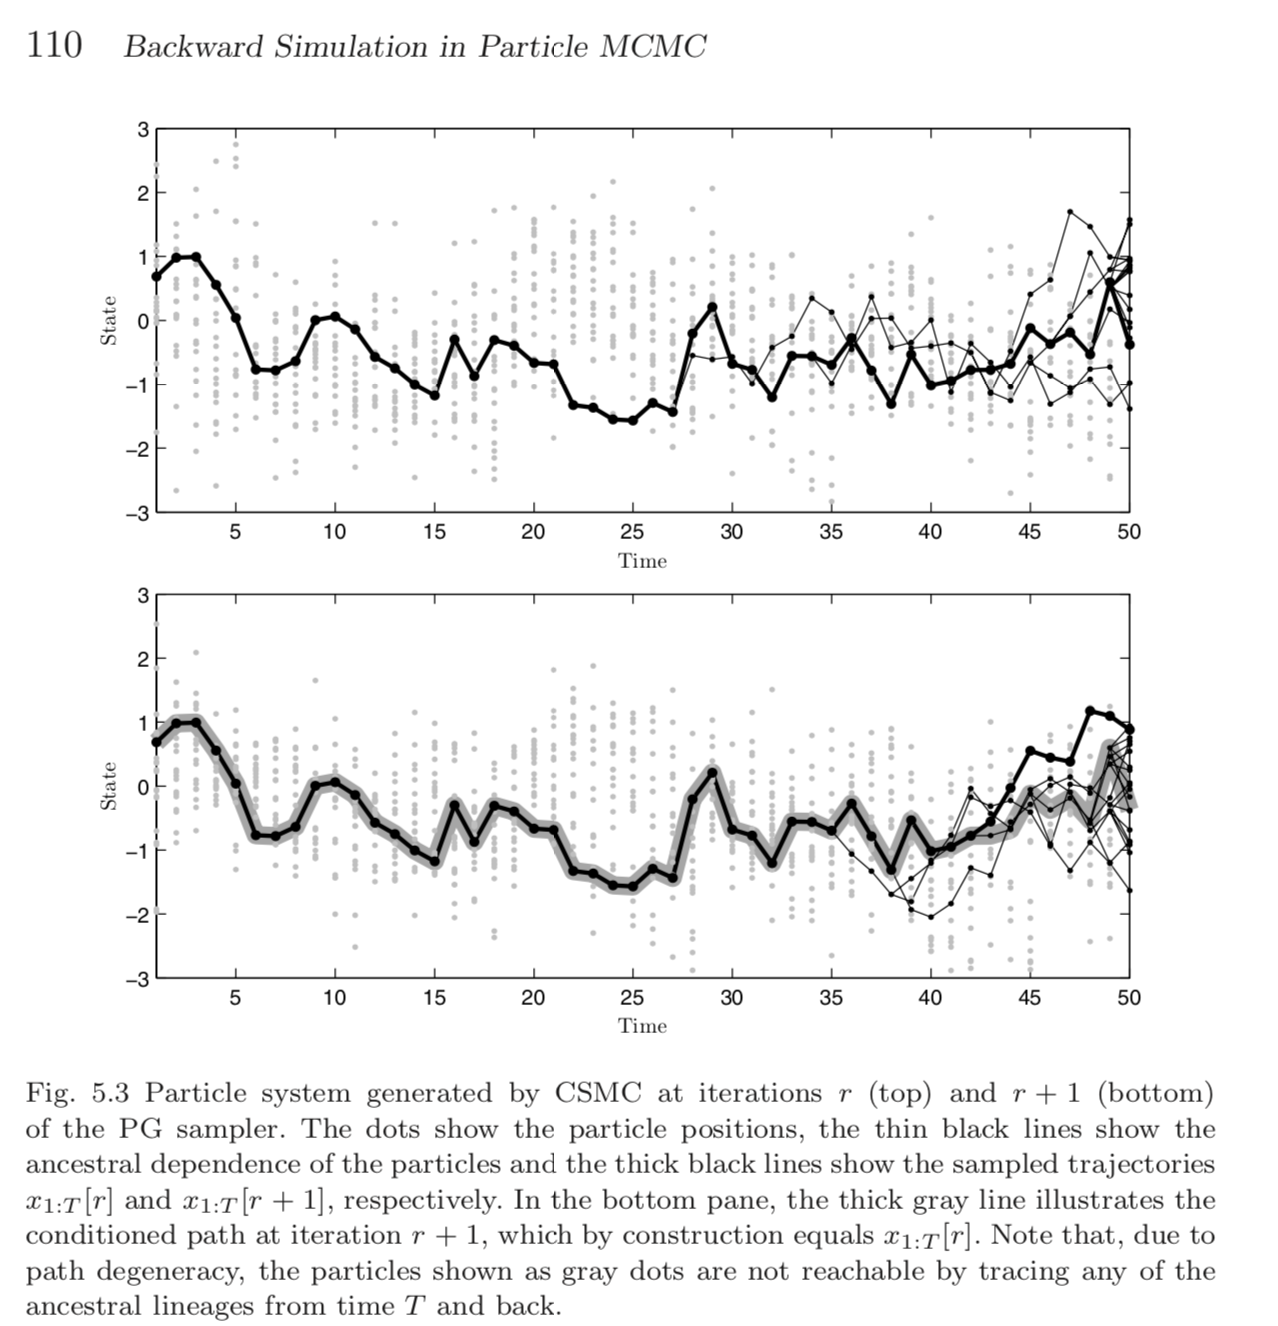
\includegraphics[width=0.8\textwidth]{plots/lindsten_figure.png}
\caption{PLACEHOLDER. Copied from \textcite{lindsten2013}.}
\label{fig:PG_ancdegen}
\end{figure}

To see why, take a look at Figure \ref{fig:PG_ancdegen}. In Figure \ref{fig:PG_ancdegen}a we have just completed the $r^{th}$ Gibbs sweep, sampling $\theta[r]$ and $x_{0:T}[r]$. For the $(r+1)^{th}$ sweep, we take as immortal trajectory $x_{0:T}^* = x_{0:T}[r]$, and run conditional SMC. Due to ancestral degeneracy, many of the resulting trajectories coalesce, and since the immortal trajectory must survive across the whole time window, they tend to coalesce onto the immortal trajectory (Figure \ref{fig:PG_ancdegen}b). Now we obtain the next sample $x_{0:T}[r+1]$ by sampling a trajectory among the $N$ we have just simulated. Whichever one we choose, it has a high amount of overlap with the immortal trajectory, i.e.\ the previous sample $x_{0:T}[r]$. This behaviour tends to repeat at every iteration, meaning the early $X$ coordinates are getting `stuck' (rarely being updated). This is clearly a problem for the mixing of the Markov chain.
\seb{Another way to explain this is that the variables defining the immortal trajectory (indices and states) are never refreshed during the Gibbs sweep - this is the explanation given in Lindsten Ch5.}
It renders the particle Gibbs algorithm impractical for any such model where the time horizon $T$ is too large: either we must run the Markov chain for longer, or increase the number of particles $N$ in the conditional SMC step, neither of which is feasible on a limited computational budget. 


\subsubsection{The solution: ancestor sampling}

An effective solution (where it is possible to implement it) was proposed by Nick Whiteley and is known as ancestor sampling.
It consists of a simple modification to the resampling step within the conditional SMC algorithm. 
In the basic CSMC algorithm, at each time step the particles are resampled by multinomial resampling according to their weights. That is, at each time $t$, each non-immortal offspring is assigned a parent as so:
\begin{equation*}
\Prob[a_t^{(j)} = i] \propto w_t^{(i)} ,
\end{equation*}
while the immortal offspring is deterministically assigned to the immortal parent.

\begin{figure}
\centering
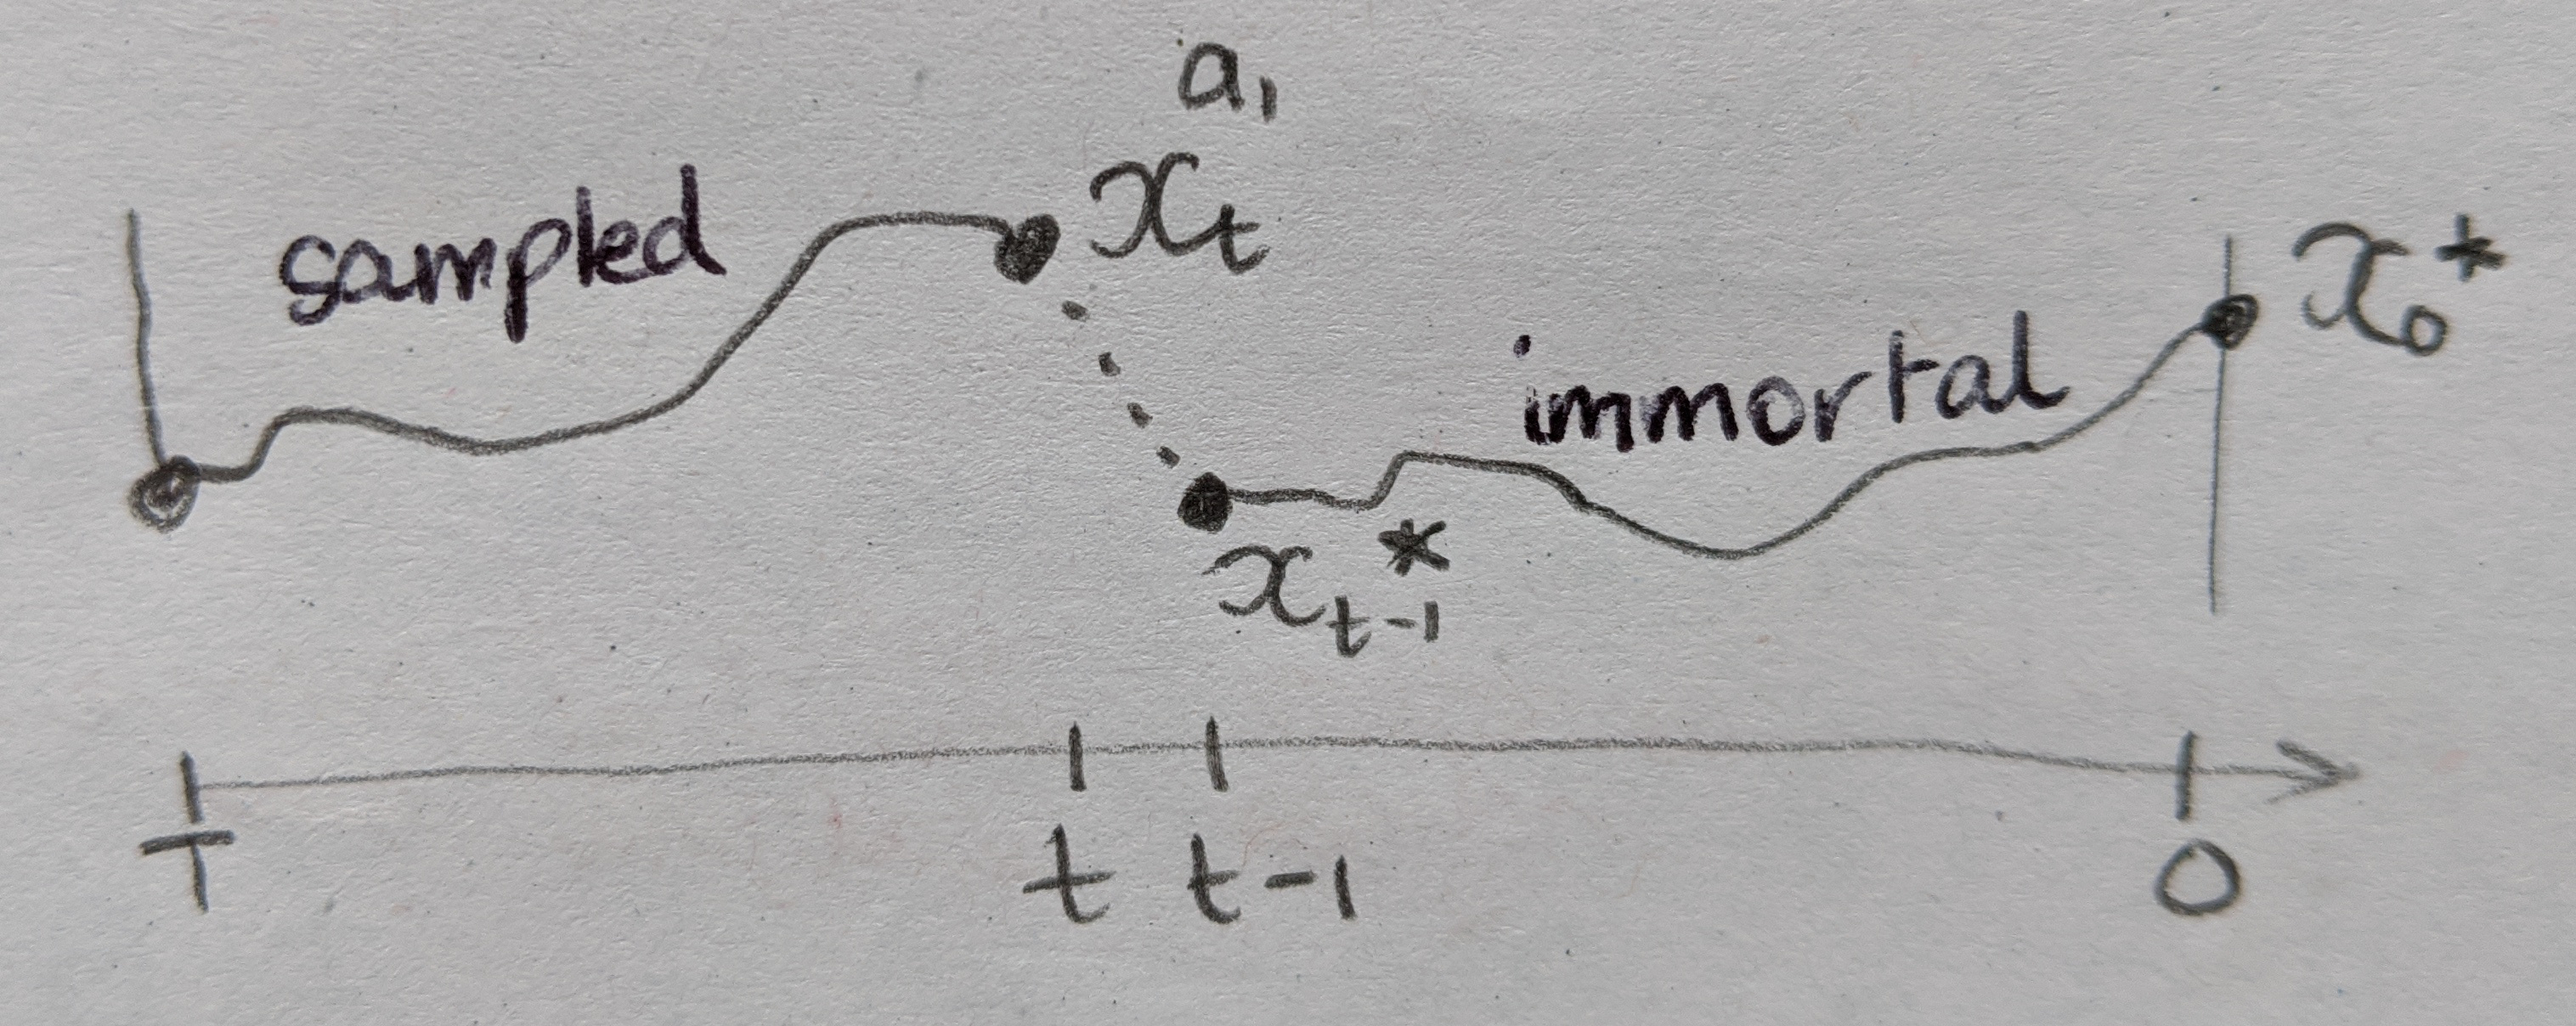
\includegraphics[width=0.8\textwidth]{plots/immresample.jpg}
\caption{PLACEHOLDER. Interpretation of a resampling weight for the immortal offspring.}
\label{fig:resample_immortal}
\end{figure}

In ancestor sampling we do the same thing, except that the immortal particle is also resampled, rather than being deterministically assigned:
\begin{equation}\label{eq:ancsamp_probs}
\Prob[a_t^{(j)} = i] \propto
\begin{cases}
w_t^{(i)} &\text{non-immortal particles}\\
w_t^{(i)} \frac{\gamma_T^\theta((x_{0:t-1}^{(i)}, x_{t:T}^*))}{\gamma_{t-1}^\theta(x_{0:t-1}^{(i)})} &\text{immortal particle} .
\end{cases}
\end{equation}
The ratio of $\gamma$s can be interpreted as the conditional probability of the trajectory continuing with $x_{t:T}^*$ given is starts with $x_{0:t-1}^{(i)}$ (see Figure \ref{fig:resample_immortal}).
Using the structure of the hidden Markov model defined earlier, we can rewrite the ratio
\begin{equation*}
\frac{\gamma_T^\theta((x_{0:t-1}^{(i)}, x_{t:T}^*))}{\gamma_{t-1}^\theta(x_{0:t-1}^{(i)})}
\propto f_\theta(x_t^* \mid x_{t-1}^{(i)}) g_\theta(y_t \mid x_t^*) \prod_{s=t}^T f_\theta(x_r^* \mid x_{r-1}^*) g_\theta(y_r \mid x_r^*)
\propto f_\theta(x_t^* \mid x_{t-1}^{(i)}) .
\end{equation*}
\seb{Should the first propto actually be equality?}
So it looks like it should also be pretty easy to implement ancestor sampling for our model. \seb{Write down the pseudocode to prove it?}
The only catch is that we need to be able to evaluate $f_\theta$ pointwise, whereas in the basic algorithm we only need to draw samples from $f_\theta$. This will rule out ancestor sampling in some applications.


\subsubsection{Why ancestor sampling works}

Ancestor sampling is backward sampling, but only for the immortal trajectory. (It isn't possible to do backward sampling during the forward sweep for any except the immortal trajectory - see that we can't evaluate the required $\gamma$s without knowing the future states, which are known only for the immortal trajectory.)
We know that backward sampling (on all trajectories, in a separate backward sweep) eradicates ancestral degeneracy. But we've only backward-sampled one trajectory, leaving the other $N-1$ trajectories to do their coalescing thing.

The important point is that ancestor sampling does not prevent ancestral degeneracy (it mitigates it a tiny bit like $1/N$). Ancestral degeneracy is pretty much as severe as ever; the difference is that the trajectories no longer coalesce preferentially onto the immortal trajectory. There is no longer an immortal trajectory to coalesce onto. An illustration of this can be seen in Figure \ref{fig:whyASworks}.

\begin{figure}
\centering
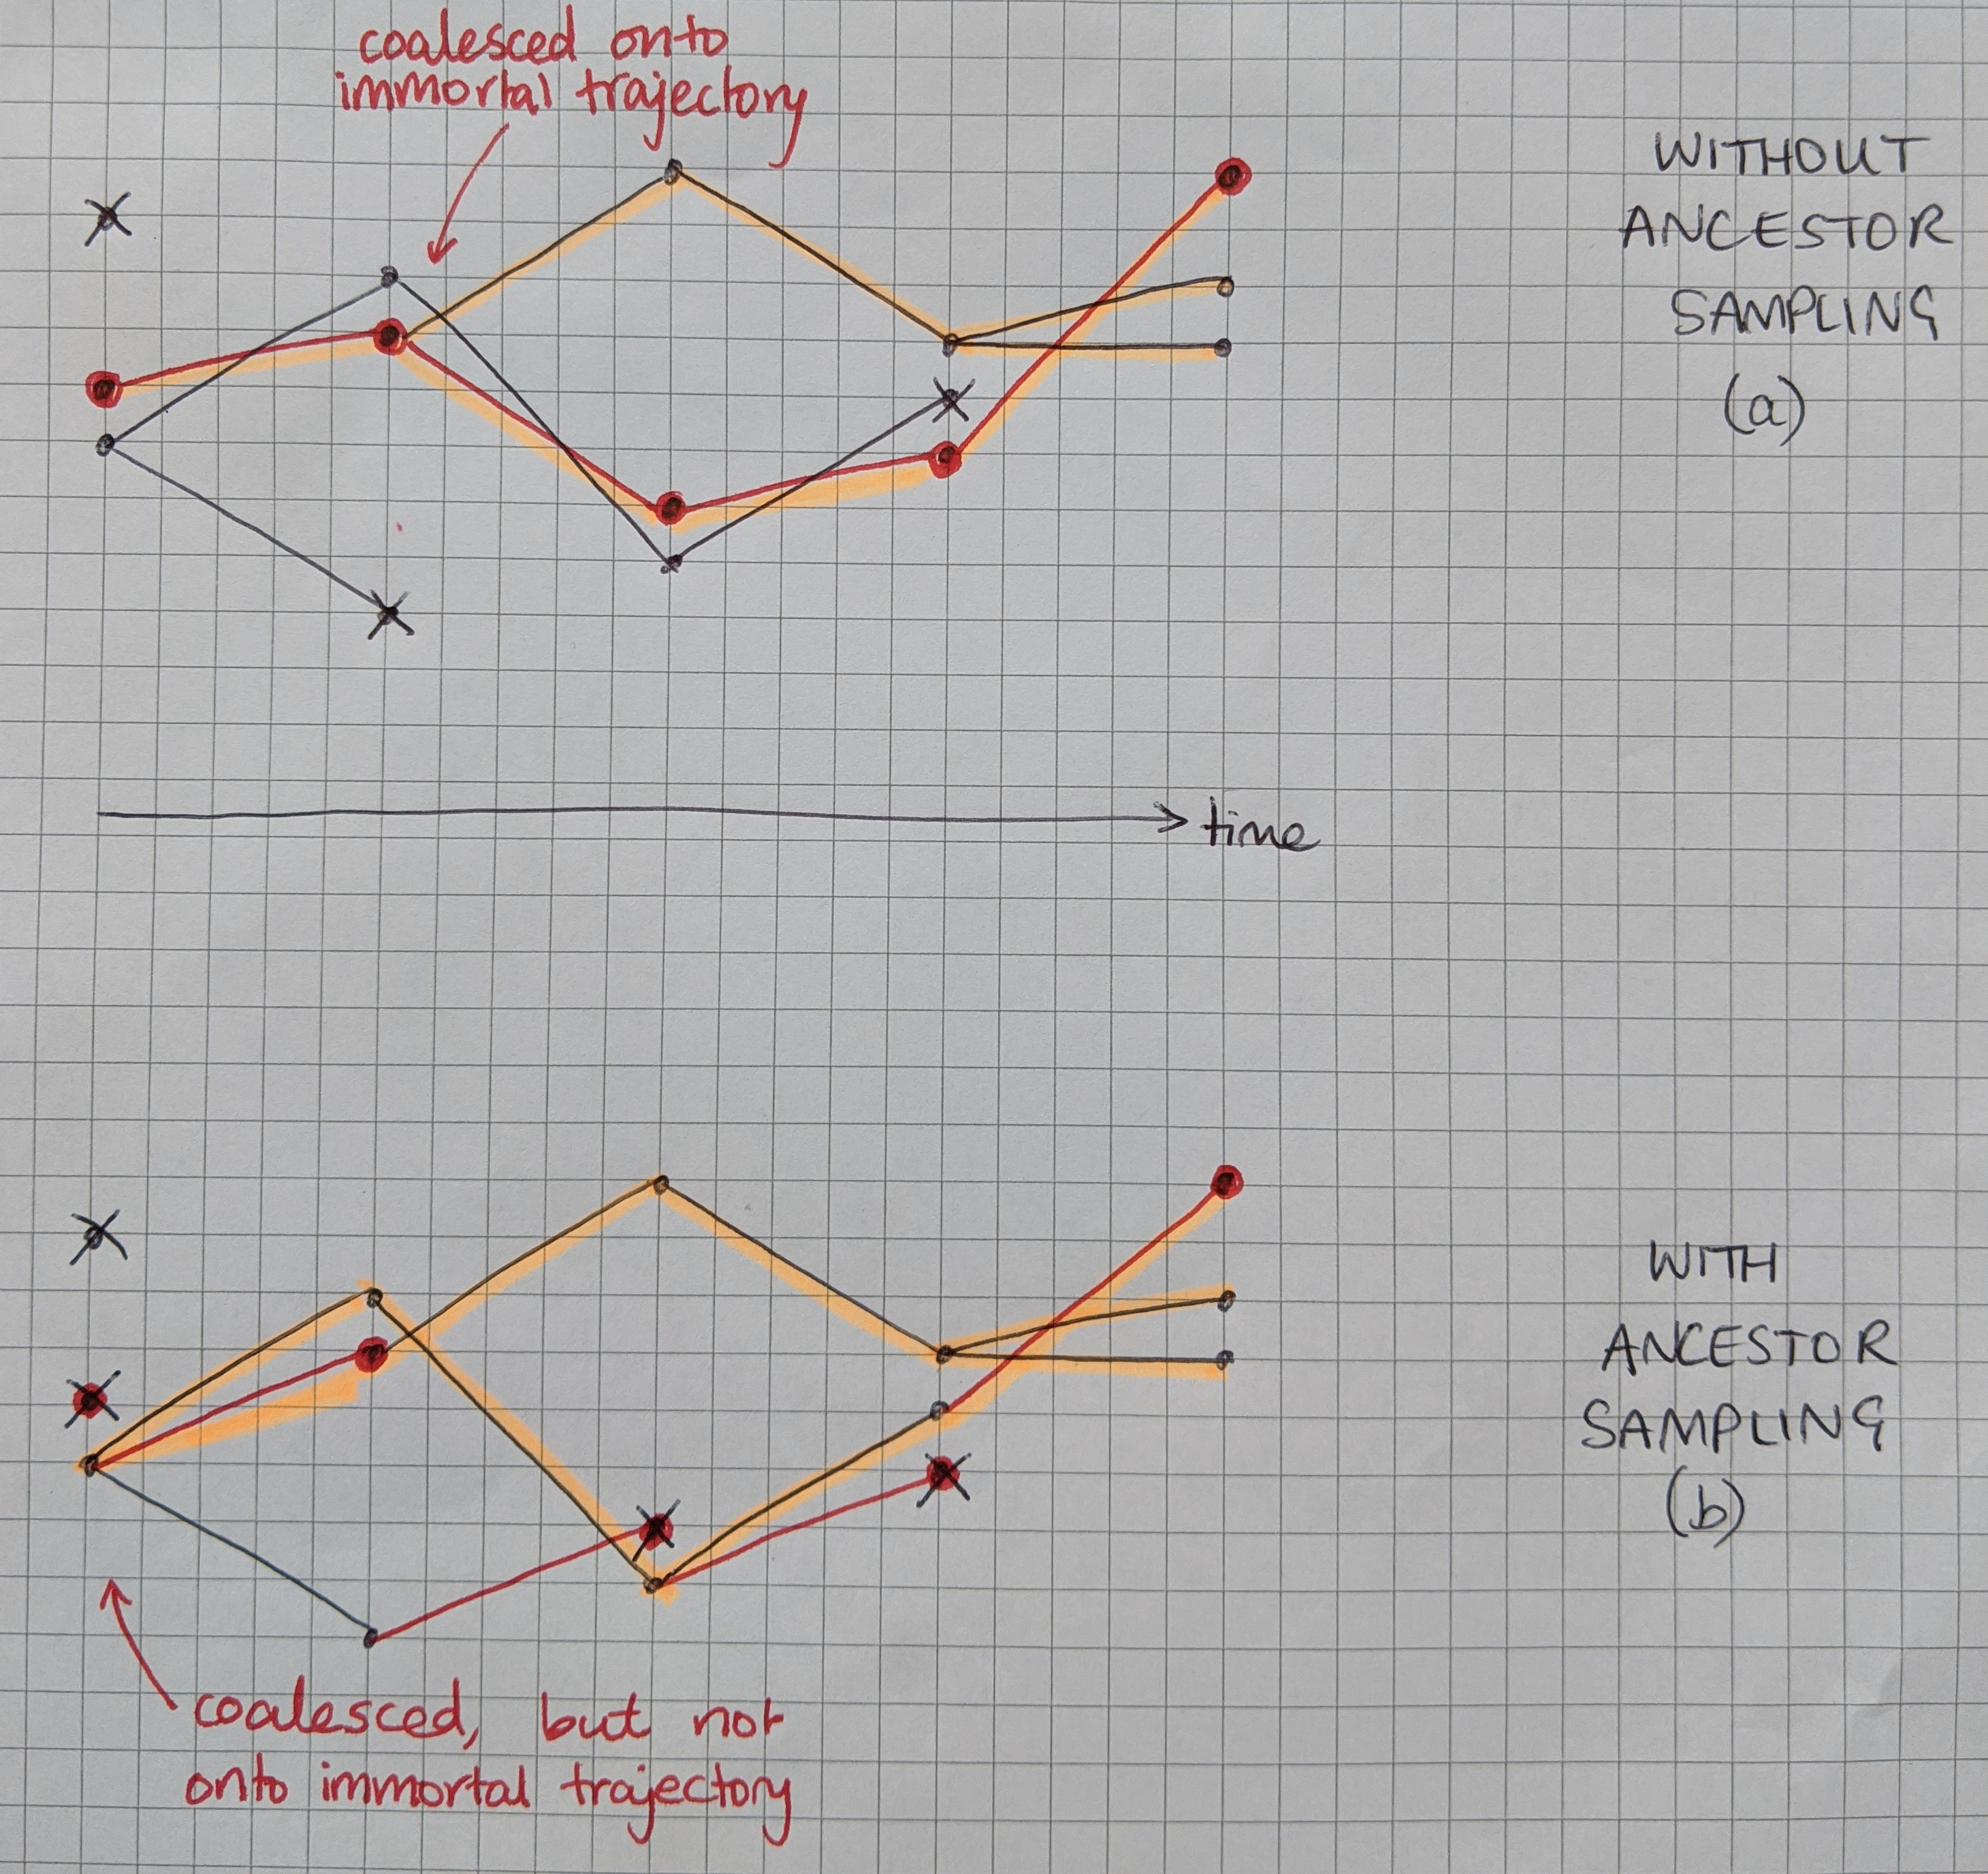
\includegraphics[width=0.8\textwidth]{plots/ancsampworks.jpg}
\caption{PLACEHOLDER. Illustration of how ancestor sampling prevents coalescence onto the immortal trajectory.}
\label{fig:whyASworks}
\end{figure}

Remember, the problem with ancestral degeneracy in particle Gibbs was that it induced strong autocorrelation among consecutive samples of $X_{0:T}$. It isn't a problem that the trajectories coalesce, as long as the thing they coalesce to is able to move, readily exploring the state space. This is achieved with ancestor sampling.

\seb{Why is ancestor sampling even a valid thing to do (i.e. still targetting the right thing)? Extended state space argument?(I think there is one in Lindsten Ch5). No need to go into it here unless there is a simple intuitive explanation to put the reader's mind at rest.}

\chapter{Limits}

%%% choose an epigraph to go here

\section{Encoding genealogies \seb{$\sim$} }

\subsection{The genealogical process \seb{$\checkmark$} }
Before we can analyse genealogies, we need a way to encode them.
The encoding will only include the information relevant to the sample genealogy, namely which lineages coalesce at which times. Information about particle positions and ``killed'' particles is ignored.

Let $\mathcal{P}_n$ be the space of partitions on $\{1,\dots,n\}$.
For convenience, we now label time in reverse, so the terminal particles are at time 0, their parents are at time 1, and so on.
Consider a randomly chosen sample of $n$ terminal particles among a total of $N$ particles, and label the sampled particles $1,\dots,n$.
The genealogical process $(G_t^{(n,N)})_{t\in\mathbb{N}_0}$ for this sample is the $\mathcal{P}_n$-valued stochastic process such that labels $i$ and $j$ are in the same block of the partition $G_t^{(n,N)}$ if and only if terminal particles $i$ and $j$ have a common ancestor at time $t$ (i.e.\ $t$ generations back).

A formulation where $G_t^{(n,N)}$ takes values in the space of equivalence relations from $[n]$ to $[n]$ is sometimes used \parencite[e.g.][]{mohle1999}; interpreting partition blocks as equivalence classes, this formulation is equivalent to ours.

The initial (time 0) value of the process is the partition of singletons $G_0^{(n,N)} = \{ \{1\}, \dots, \{n\} \}$, since all of the terminal particles are separate.
The only possible non-identity transitions are those that merge some blocks of the partition; this encodes the coalescence of the corresponding lineages.
The trivial partition $\{ \{1,\dots,n\} \}$ is therefore an absorbing state, corresponding to all lineages in the sample having coalesced (i.e.\ the MRCA has been reached).
The construction of the genealogical process from the resampling indices is illustrated in Figure \ref{fig:encoding_genealogy}.

\begin{figure}
\centering
\subfloat[Resampling relationships]{
\begin{tikzpicture}
% grid of particles
\filldraw (0,0) circle (2pt);
\filldraw (0.75,0) circle (2pt);
\filldraw (1.5,0) circle (2pt);
\filldraw (2.25,0) circle (2pt);
\filldraw (3,0) circle (2pt);
\filldraw (3.75,0) circle (2pt);
\filldraw (0,1) circle (2pt);
\filldraw (0.75,1) circle (2pt);
\filldraw (1.5,1) circle (2pt);
\filldraw (2.25,1) circle (2pt);
\filldraw (3,1) circle (2pt);
\filldraw (3.75,1) circle (2pt);
\filldraw (0,2) circle (2pt);
\filldraw (0.75,2) circle (2pt);
\filldraw (1.5,2) circle (2pt);
\filldraw (2.25,2) circle (2pt);
\filldraw (3,2) circle (2pt);
\filldraw (3.75,2) circle (2pt);
\filldraw (0,3) circle (2pt);
\filldraw (0.75,3) circle (2pt);
\filldraw (1.5,3) circle (2pt);
\filldraw (2.25,3) circle (2pt);
\filldraw (3,3) circle (2pt);
\filldraw (3.75,3) circle (2pt);
\filldraw (0,4) circle (2pt);
\filldraw (0.75,4) circle (2pt);
\filldraw (1.5,4) circle (2pt);
\filldraw (2.25,4) circle (2pt);
\filldraw (3,4) circle (2pt);
\filldraw (3.75,4) circle (2pt);
% resampling arrows % generation 4 to 5
\draw[->] (0.75,0.9)--(0,0.1);
\draw[->] (0.75,0.9)--(0.75,0.1);
\draw[->] (0.75,0.9)--(1.5,0.1);
\draw[->] (2.25,0.9)--(2.25,0.1);
\draw[->] (3,0.9)--(3,0.1);
\draw[->] (3.75,0.9)--(3.75,0.1);
% resampling arrows % generation 3 to 4
\draw[->] (0,1.9)--(0,1.1);
\draw[->] (0.75,1.9)--(0.75,1.1);
\draw[->] (1.5,1.9)--(1.5,1.1);
\draw[->] (2.25,1.9)--(2.25,1.1);
\draw[->] (2.25,1.9)--(3,1.1);
\draw[->] (3,1.9)--(3.75,1.1);
% resampling arrows % generation 2 to 3
\draw[->] (0,2.9)--(0,2.1);
\draw[->] (1.5,2.9)--(0.75,2.1);
\draw[->] (1.5,2.9)--(1.5,2.1);
\draw[->] (2.25,2.9)--(2.25,2.1);
\draw[->] (2.25,2.9)--(3,2.1);
\draw[->] (3.75,2.9)--(3.75,2.1);
% resampling arrows % generation 1 to 2
\draw[->] (0.75,3.9)--(0,3.1);
\draw[->] (0.75,3.9)--(0.75,3.1);
\draw[->] (1.5,3.9)--(1.5,3.1);
\draw[->] (1.5,3.9)--(2.25,3.1);
\draw[->] (3.75,3.9)--(3,3.1);
\draw[->] (3.75,3.9)--(3.75,3.1);
% fudge bottom space
\node[anchor=north] at (0,0) {\textcolor{white}{\footnotesize{1}}};
\end{tikzpicture}
\label{fig:encoding_a}
}
\hspace{0.9cm}
\subfloat[Genealogy of terminal particles]{
\begin{tikzpicture}
% horizontal time lines
\draw[gray,dotted] (-0.2,0)--(4.05,0);
\draw[gray,dotted] (-0.2,1)--(4.05,1);
\draw[gray,dotted] (-0.2,2)--(4.05,2);
\draw[gray,dotted] (-0.2,3)--(4.05,3);
\draw[gray,dotted] (-0.2,4)--(4.05,4);
% tree
\draw[thick] (0.75,0)--(0.75,4);
\draw[thick] (0,0)--(0,1);
\draw[thick] (1.5,0)--(1.5,1);
\draw[thick] (0,1)--(1.5,1);
\draw[thick] (2.25,0)--(2.25,2);
\draw[thick] (3,0)--(3,2);
\draw[thick] (2.25,2)--(3,2);
\draw[thick] (2.625,2)--(2.625,3);
\draw[thick] (3.75,0)--(3.75,3);
\draw[thick] (2.625,3)--(3.75,3);
\draw[thick] (3.1875,3)--(3.1875,4);
\draw[thick] (0.75,4)--(3.1875,4);
% lineage labels
\node[anchor=north] at (0,0) {\footnotesize{1}};
\node[anchor=north] at (0.75,0) {\footnotesize{2}};
\node[anchor=north] at (1.5,0) {\footnotesize{3}};
\node[anchor=north] at (2.25,0) {\footnotesize{4}};
\node[anchor=north] at (3,0) {\footnotesize{5}};
\node[anchor=north] at (3.75,0) {\footnotesize{6}};
% partition labels
\node[anchor=west] at (4.1,0) {\textcolor{gray}{\footnotesize{$G_0 = \{ \{1\}, \{2\}, \{3\}, \{4\}, \{5\}, \{6\} \}$}}};
\node[anchor=west] at (4.1,1) {\textcolor{gray}{\footnotesize{$G_1 = \{ \{1,2,3\}, \{4\}, \{5\}, \{6\} \}$}}};
\node[anchor=west] at (4.1,2) {\textcolor{gray}{\footnotesize{$G_2 = \{ \{1,2,3\}, \{4,5\}, \{6\} \}$}}};
\node[anchor=west] at (4.1,3) {\textcolor{gray}{\footnotesize{$G_3 = \{ \{1,2,3\}, \{4,5,6\} \}$}}};
\node[anchor=west] at (4.1,4) {\textcolor{gray}{\footnotesize{$G_4 = \{ \{1,2,3,4,5,6\} \}$}}};
\end{tikzpicture}
\label{fig:encoding_b}
}
\caption[Illustration of how the sample genealogy is encoded]{Illustration of how the sample genealogy is encoded. \subref{fig:encoding_a} Relationships induced by resampling with six particles over four iterations. \subref{fig:encoding_b} The genealogy of the terminal particles, labelled with the value of the genealogical process $G_t$ at each time.}
\label{fig:encoding_genealogy}
\end{figure}


\subsection{Time scale \seb{$\checkmark$} }
In order to get a continuous limit, we scale time by a function $\tau_N(\cdot)$. In the population genetics literature the time scale is typically deterministic (Section~\ref{sec:popgenmodels}), but in our case $\tau_N$ depends on the offspring counts and is therefore random.
To define the time scale we first define the pair merger rate
\begin{equation}\label{eq:defn_cN}
c_N(t) := \frac{1}{(N)_2} \sum_{i=1}^N (\nu_t^{(i)})_2 .
\end{equation}
This is the probability, conditional on $\nu_t^{(1:N)}$, that a randomly chosen pair of lineages in generation $t$ merges exactly one generation back.
To achieve the limiting pair merger rate of 1, as in the $n$-coalescent, we rescale time by the generalised inverse
\begin{equation}\label{eq:defn_tauN}
\tau_N(t) := \inf \left\{ s \geq 1 : \sum_{r=1}^s c_N(r) \geq t \right\} .
\end{equation}
The function $\tau_N$ maps continuous to discrete time, providing the link between the discrete-time SMC dynamics and the continuous-time Kingman limit.
We will also need the following quantity, which is an upper bound on the rate of multiple mergers (three or more lineages merging, or two or more simultaneous pairwise mergers):
\begin{equation}\label{eq:defn_DN}
D_N(t) := \frac{1}{N(N)_2} \sum_{i=1}^N (\nu_t^{(i)})_2
        \left\{ \nu_t^{(i)} + \frac{1}{N} \sum_{j\neq i} (\nu_t^{(j)})^2 \right\} .
\end{equation} 
%Let $\nu_t^{(i)}$ be the number of offspring in generation $t$ of particle $i$ ($t \in \mathbb{N}$, $i = 1,\dots, N$).
%Let $(\mathcal{F}_t)$ be the reverse-time filtration generated by the offspring counts.
Some basic properties are given in Proposition~\ref{thm:cN_properties}.
\begin{prop}[Properties of $c_N$]\label{thm:cN_properties}
For all $t\in\mathbb{N}$, $t^\prime > s^\prime >0$,
\begin{enumerate}[label=(\alph*)]
\item \label{item:cN_property1} \hspace{5pt}
    $\begin{aligned}
    c_N(t) , D_N(t) \in [0,1]
    \end{aligned}$
\item \label{item:cN_property2} \hspace{5pt}
    $\begin{aligned}
    D_N(t) \leq c_N(t)
    \end{aligned}$
\item \label{item:cN_property3} \hspace{5pt}
    $\begin{aligned}
    c_N(t)^2 \leq c_N(t) 
    \end{aligned}$
\item \label{item:cN_property4} \hspace{5pt}
    $\begin{aligned}
    t^\prime
    \leq \sum_{r=1}^{\tau_N(t^\prime)} c_N(r) 
    \leq t^\prime +1 .
    \end{aligned}$
\item \label{item:cN_property5} \hspace{5pt}
    $\begin{aligned}
    t^\prime - s^\prime -1
    \leq \sum_{r=\tau_N(s^\prime)+1}^{\tau_N(t^\prime)} c_N(r) 
    \leq t^\prime - s^\prime +1 .
    \end{aligned}$
\item \label{item:cN_property6} \hspace{5pt}
    $\begin{aligned}
    \tau_N(t^\prime) \geq t^\prime
    \end{aligned}$
\end{enumerate}
%\begin{align}
%& c_N(t) , D_N(t) \in [0,1] \label{eq:cN_property1}\\
%& D_N(t) \leq c_N(t) \label{eq:cN_property2}\\
%& c_N(t)^2 \leq c_N(t) \label{eq:cN_property3}\\
%& t^\prime \leq \sum_{r=1}^{\tau_N(t^\prime)} c_N(r) \leq t^\prime +1 . \label{eq:cN_property4}
%\end{align}
\end{prop}

\begin{proof}
\textbf{\ref{item:cN_property1}}  $c_N(t)$ and $D_N(t)$ are clearly non-negative. Both are maximised when one of the offspring counts is equal to $N$ and the rest are zero, in which case $c_N(t) = D_N(t) = 1$.\\
\textbf{\ref{item:cN_property2}} As outlined in \textcite[p.9]{koskela2018},
\begin{align*}
D_N(t) &:= \frac{1}{(N)_2} \sum_{i=1}^N (\nu_t^{(i)})_2 \frac{1}{N} \left\{  \nu_t^{(i)} + \frac{1}{N} \sum_{j\neq i}^N (\nu_t^{(j)})^2 \right\} \\
&\leq \frac{1}{(N)_2} \sum_{i=1}^N (\nu_t^{(i)})_2 \frac{1}{N} \left\{  \nu_t^{(i)} + \frac{1}{N} \sum_{j\neq i}^N N \nu_t^{(j)} \right\} \\
&= \frac{1}{(N)_2} \sum_{i=1}^N (\nu_t^{(i)})_2 \frac{1}{N} \left\{ \sum_{j =1}^N \nu_t^{(j)} \right\}
\leq \frac{1}{(N)_2} \sum_{i=1}^N (\nu_t^{(i)})_2
= c_N(t) .
\end{align*}
\textbf{\ref{item:cN_property3}} is immediate given \ref{item:cN_property1}.\\
\textbf{\ref{item:cN_property4}} follows directly from the definition of $\tau_N$ in \eqref{eq:defn_tauN}.\\
\textbf{\ref{item:cN_property5}} Writing
\begin{equation*}
\sum_{r=\tau_N(s^\prime)+1}^{\tau_N(t^\prime)} c_N(r)
= \sum_{r=1}^{\tau_N(t^\prime)} c_N(r) 
        - \sum_{r=1}^{\tau_N(s^\prime)} c_N(r) ,
\end{equation*}
the result follows by applying \ref{item:cN_property4} to both sums.\\
\textbf{\ref{item:cN_property6}} follows from \ref{item:cN_property1} and the definition of $\tau_N$ in \eqref{eq:defn_tauN}.
\end{proof}


Another useful property is the following, taken from \textcite[Lemma 2]{koskela2018}. There the special case $f(r) \equiv c_N(r)$ is proved, but the authors remark that the result also holds for other choices of $f$. Here we state the result in full generality.

\begin{lemma}\label{thm:kjjslemma2}
Fix $t>0$.
Let $(\mathcal{F}_r)$ be the backwards-in-time filtration generated by the offspring counts $\nu_r^{(1:N)}$ at each generation $r$,
and let $f(r)$ be any deterministic function of $\nu_r^{(1:N)}$ that is non-negative and bounded. In particular, for all $r$ there exists $B<\infty$ such that $0\leq f(r) \leq B$.
Then
\begin{equation*}
\E \left[ \sum_{r=1}^{\tau_N(t)} f(r) \right] 
= \E \left[ \sum_{r=1}^{\tau_N(t)} \E [ f(r) \mid \mathcal{F}_{r-1} ] \right] .
\end{equation*}
\end{lemma}

\begin{proof}
Define 
\begin{equation*}
M_s 
:= \sum_{r=1}^s \left\{ f(r) - \E [ f(r) \mid \mathcal{F}_{r-1} ] \right\} .
\end{equation*}
It is easy to establish that $(M_s)$ is a martingale with respect to $(\mathcal{F}_s)$, and $M_0 = 0$. 
Now fix $K\geq 1$ and note that $\tau_N(t) \wedge K$ is a bounded $\mathcal{F}_t$-stopping time.
Hence we can apply the optional stopping theorem:
\begin{align*}
\E [M_{\tau_N(t) \wedge K} ]
&= \E \left[ \sum_{r=1}^{\tau_N(t) \wedge K} \left\{ f(r) 
        - \E [ f(r) \mid \mathcal{F}_{r-1} ] \right\} \right] \\
&= \E \left[ \sum_{r=1}^{\tau_N(t) \wedge K} f(r) \right]
        - \E \left[ \sum_{r=1}^{\tau_N(t) \wedge K} 
        \E [ f(r) \mid \mathcal{F}_{r-1} ] \right]
=0 .
\end{align*}
Since this holds for all $K\geq 1$,
\begin{equation*}
\lim_{K\to\infty} \E \left[ \sum_{r=1}^{\tau_N(t) \wedge K} f(r) \right]
= \lim_{K\to\infty} \E \left[ \sum_{r=1}^{\tau_N(t) \wedge K} 
        \E [ f(r) \mid \mathcal{F}_{r-1} ] \right] .
\end{equation*}
The monotone convergence theorem allows the limit to pass inside the expectation on each side (since increasing $K$ can only increase each sum, by possibly adding non-negative terms). Hence
\begin{align*}
\E \left[ \sum_{r=1}^{\tau_N(t)} f(r) \right]
&= \E \left[ \lim_{K\to\infty} \sum_{r=1}^{\tau_N(t) \wedge K} f(r) \right]
= \E \left[ \lim_{K\to\infty} \sum_{r=1}^{\tau_N(t) \wedge K} 
        \E [ f(r) \mid \mathcal{F}_{r-1} ] \right] \\
&= \E \left[ \sum_{r=1}^{\tau_N(t)} 
        \E [ f(r) \mid \mathcal{F}_{r-1} ] \right]
\end{align*}
which concludes the proof.
\end{proof}



\subsection{Transition probabilities \seb{$\sim$} }
\draft{Present bounds on $p_{\xi\xi}$ that will be used later (keeping big-O terms explicit where possible).}

Let $\mathcal{P}_n$ be the space of partitions of $\{1,\dots,n\}$, and denote by $\Delta$ the partition of singletons $\{ \{1\},\dots, \{n\} \}$.
For any $\xi, \eta \in \mathcal{P}_n$ and $t\in\mathbb{N}$, let $p_{\xi\eta}(t)$ denote the conditional transition probabilities of the genealogical process given $\nu_t^{(1:N)}$ ($t\in\mathbb{N}$, $\xi, \eta \in \mathcal{P}_n$).
The transition probability $p_{\xi\eta}(t)$ can only be non-zero when $\eta$ can be obtained from $\xi$ by merging some blocks of $\xi$.
Ordering the blocks by their least element, denote by $b_i$ the number of blocks of $\xi$ that merge to form block $i$ in $\eta$ ($i \in \{1,\dots, |\eta|\}$). Hence $b_1 + \cdots + b_{|\eta|} = |\xi|$.
Then the transition probability is given by
\begin{equation}\label{eq:defn_pxieta}
p_{\xi\eta}(t) 
:= \frac{1}{(N)_{|\xi|}} \sum_{\substack{i_1 \neq \cdots \neq i_{|\eta|} \\ =1}}^N
        (\nu_t^{(i_1)})_{b_1} \cdots (\nu_t^{(i_{|\eta|})})_{b_{|\eta|}} .
\end{equation}
We will only need to work directly with the identity transition probabilities $p_{\xi\xi}(t)$.
Upper and lower bounds on these probabilities are presented in Propositions \ref{thm:pDelta_LB} and \ref{thm:pDelta_UB}.
\begin{prop}[Lower bound on identity transition probabilities]\label{thm:pDelta_LB}
Let $\xi \in \mathcal{P}_n$, $N>2$. Then
\begin{equation*}
p_{\xi\xi}(t)
\geq 1 - \binom{|\xi|}{2} \frac{N^{n-2}}{(N-2)_{n-2}} \left[ c_N(t) + B_{|\xi|} D_N(t) \right]
\end{equation*}
where 
\begin{equation*}
B_{|\xi|} = K (|\xi|-1)! (|\xi|-2) \exp( 2 \sqrt{2(|\xi|-2)} )
\end{equation*}
for some $K>0$ that does not depend on $|\xi|$.
\end{prop}
\seb{For weak convergence proof, refer to this proposition but rewrite the inequality using $\xi = \Delta$ and $\alpha_n$, to provide a local target for cross-referencing. Similarly for UB.}
\begin{proof}
%The proof follows \textcite[Proof of Lemma 3.6]{brown2021}, but keeping the terms in $N$ explicit. --- I don't need to refer to BJJK as it's part of my work; just reproduce BJJK's workings nice and verbosely here :)
We have the following expression for $p_{\xi\xi}(t)$, by subtracting all possible non-identity transitions (the omitted $k=|\xi|$ term would count identity transitions):
\begin{equation*}
p_{ \xi \xi }( t ) 
= 1 - \frac{ 1 }{ ( N )_{ | \xi | } } \sum_{ k = 1 }^{ | \xi | - 1 } 
        \sum_{ \substack{ b_1 \geq \ldots \geq b_k = 1 
        \\ b_1 + \ldots + b_k = | \xi | } }^{ | \xi | } 
        \frac{ | \xi |! }{ \prod_{ j = 1 }^{ | \xi | } ( j ! )^{ \kappa_j } \kappa_j ! } 
        \sum_{ \substack{ i_1 \neq \ldots \neq i_k = 1 \\ \text{all distinct} } }^N 
        ( \nu_t^{ ( i_1 ) } )_{ b_1 } \ldots ( \nu_t^{ ( i_k ) } )_{ b_k },
\end{equation*}
where $\kappa_i = |\{ j : b_j = i \}|$ is the multiplicity of mergers of size $i$ ($\kappa_1$ counts non-merger events, and we have the identity $\kappa_1 + 2 \kappa_2 + \cdots + | \xi | \kappa_{ | \xi | } = | \xi |$).
The combinatorial factor is the number of partitions of a sequence of length $|\xi|$  having $\kappa_j$ subsequences of length $j$ for each $j$ \parencite[Equation (11)]{fu2006}.

We separate the $k=|\xi|-1$ term (which counts single pair mergers), for which $(b_1, b_2, \dots, b_{|\xi|-1}) = (2,1,\dots,1)$ and
\begin{equation*}
\frac{ | \xi |! }{ \prod_{ j = 1 }^{ | \xi | } ( j ! )^{ \kappa_j } \kappa_j ! }
= \binom{|\xi|}{2} .
\end{equation*}
For the remaining terms we use
\begin{equation*}
\frac{ | \xi |! }{ \prod_{ j = 1 }^{ | \xi | } ( j ! )^{ \kappa_j } \kappa_j ! }
\leq |\xi|! .
\end{equation*}
Thus
\begin{align*}
p_{ \xi \xi }( t ) 
&\geq 1 - \frac{ 1 }{ ( N )_{ | \xi | } } \binom{|\xi|}{2}
        \sum_{ \substack{ i_1 \neq \ldots \neq i_{|\xi|-1} = 1 \\ \text{all distinct} } }^N 
        ( \nu_t^{ ( i_1 ) } )_2 \nu_t^{(i_2)} \ldots \nu_t^{ ( i_{|\xi|-1} ) } \\
    &\qquad- \frac{ 1 }{ ( N )_{ | \xi | } } \sum_{ k = 1 }^{ | \xi | - 1 } 
        \sum_{ \substack{ b_1 \geq \ldots \geq b_k = 1 
        \\ b_1 + \ldots + b_k = | \xi | } }^{ | \xi | } |\xi|!
        \sum_{ \substack{ i_1 \neq \ldots \neq i_k = 1 \\ \text{all distinct} } }^N 
        ( \nu_t^{ ( i_1 ) } )_{ b_1 } \ldots ( \nu_t^{ ( i_k ) } )_{ b_k }
\end{align*}
Now, for the $k=|\xi|-1$ term we use the bound
\begin{equation*}
\sum_{ i_1 \neq \ldots \neq i_{ | \xi | - 1 } = 1 }^N 
        ( \nu_t^{ ( i_1 ) } )_2 \nu_t^{ ( i_2 ) } \ldots \nu_t^{ ( i_{ | \xi | - 1 } ) }
\leq N^{ | \xi | - 2 } \sum_{ i = 1 }^N ( \nu_t^{ ( i ) } )_2
\end{equation*}
while for the other terms we have \parencite[similarly to][Lemma 1 Case 3]{koskela2018}
\begin{align*}
\sum_{ \substack{ i_1 \neq \ldots \neq i_k = 1 \\ \text{all distinct} } }^N &( \nu_t^{ ( i_1 ) } )_{ b_1 } \ldots ( \nu_t^{ ( i_k ) } )_{ b_k } \leq \sum_{ i = 1 }^N ( \nu_t^{ ( i ) } )_2 \Bigg( N^{ | \xi | - 2 } - \sum_{ \substack{ j_1 \neq \ldots \neq j_{ | \xi | - 2 } = 1 \\ \text{all distinct and } \neq i } }^N \nu_t^{ ( j_1 ) } \ldots \nu_t^{ ( j_{ | \xi | - 2 } ) } \Bigg) \\
&\leq \sum_{ i = 1 }^N ( \nu_t^{ ( i ) } )_2 \Bigg\{ N^{ | \xi | - 2 } - ( N - \nu_t^{ ( i ) } )^{ | \xi | - 2 } + \binom{ | \xi | - 2 }{ 2 } \sum_{ j \neq i } ( \nu_t^{ ( j ) } )^2 \Bigg( \sum_{ k \neq i } \nu_t^{ ( k ) } \Bigg)^{ | \xi | - 4 } \Bigg\} \\
&\leq \sum_{ i = 1 }^N ( \nu_t^{ ( i ) } )_2 \Bigg\{ ( | \xi | - 2 ) \nu_t^{ ( i ) } N^{ | \xi | - 3 } + \binom{ | \xi | - 2 }{ 2 } \sum_{ j \neq i } ( \nu_t^{ ( j ) } )^2 N^{ | \xi | - 4 } \Bigg\},
\end{align*}
where the last step uses $(N - x)^b \geq N^b - b x N^{ b - 1 }$ for $x \leq N$, $b \geq 0$.
Hence
\begin{align*}
p_{ \xi \xi }( t ) 
&\geq 1 - \frac{ 1 }{ ( N )_{ | \xi | } } \binom{|\xi|}{2}
        N^{ | \xi | - 2 } \sum_{ i = 1 }^N ( \nu_t^{ ( i ) } )_2 \\
    &\qquad- \frac{ N^{|\xi|-3} }{ ( N )_{ | \xi | } } |\xi|!
        \sum_{ k = 1 }^{ | \xi | - 1 } 
        \sum_{ \substack{ b_1 \geq \ldots \geq b_k = 1 
        \\ b_1 + \ldots + b_k = | \xi | } }^{ | \xi | } 
        \sum_{ i = 1 }^N ( \nu_t^{ ( i ) } )_2 
        \Bigg\{ ( | \xi | - 2 ) \nu_t^{ ( i ) } + \binom{ | \xi | - 2 }{ 2 } \frac{1}{N} 
        \sum_{ j \neq i } ( \nu_t^{ ( j ) } )^2 \Bigg\} .
\end{align*}
The summands in the last line are independent of $k, b_i$, and the number of terms in the sums over $k$ and $b_1, \dots, b_k$ is bounded by $\gamma_{|\xi|-2} (|\xi|-2)$, where $\gamma_n$ is the number of integer partitions of $n$.
By \textcite[Section 2]{hardy1918}, $\gamma_n < K e^{ 2 \sqrt{ 2 n } } / n$ for a constant $K > 0$ independent of $n$.
Thus, for $|\xi| > 2$,
\begin{align*}
p_{ \xi \xi }( t ) 
&\geq 1 - \frac{ N^{ | \xi | - 2 } }{ ( N-2 )_{ | \xi | -2} } \binom{|\xi|}{2}
        c_N(t) \\
    &\qquad- \frac{ N^{|\xi|-2} }{ ( N-2 )_{ | \xi | -2} }
        K \exp( 2 \sqrt{2(|\xi|-2)} ) |\xi|!
        \frac{1}{N(N)_2} \\
    &\hspace{4cm} \sum_{ i = 1 }^N ( \nu_t^{ ( i ) } )_2
        \Bigg\{ ( | \xi | - 2 ) \nu_t^{ ( i ) } + \binom{ | \xi | - 2 }{ 2 } \frac{1}{N} 
        \sum_{ j \neq i } ( \nu_t^{ ( j ) } )^2 \Bigg\} \\
&\geq 1 - \frac{ N^{ | \xi | - 2 } }{ ( N-2 )_{ | \xi | -2} } \binom{|\xi|}{2}
        c_N(t) \\
    &\qquad- \frac{ N^{|\xi|-2} }{ ( N-2 )_{ | \xi | -2} }
        K \exp( 2 \sqrt{2(|\xi|-2)} ) |\xi|! \binom{ |\xi|-1}{2} D_N(t) \\
&\geq 1 - \frac{ N^{ | \xi | - 2 } }{ ( N-2 )_{ | \xi | -2} } \binom{|\xi|}{2}
        \left[ c_N(t) + B_{|\xi|} D_N(t) \right]
\end{align*}
where
\begin{align*}
B_{|\xi|} 
&= \binom{|\xi|}{2}^{-1} K \exp( 2 \sqrt{2(|\xi|-2)} ) |\xi|! \binom{ |\xi|-1}{2} \\
&= K (|\xi|-1)! (|\xi|-2) \exp( 2 \sqrt{2(|\xi|-2)} ) .
\end{align*}
When $|\xi| \leq 2$, there are no terms with $k\leq |\xi|-2$, and the result is immediate.
\end{proof}


\begin{prop}[Upper bound on identity transition probabilities]\label{thm:pDelta_UB}
Let $\xi \in \mathcal{P}_n$, $N>...$ \seb{some threshold}. Then
\begin{equation*}
p_{\xi\xi}(t)
\leq 1 - \binom{|\xi|}{2} \frac{N^{n-2}}{(N-2)_{n-2}} 
        \left[ c_N(t) - B_{|\xi|}^\prime D_N(t) \right]
\end{equation*}
where $B_{|\xi|}^\prime = \binom{|\xi|-1}{2}$.
\end{prop}

\begin{proof}
The proof follows \textcite[Proof of Lemma 1 Case 1]{koskela2018} but with the terms in $N$ kept explicit. \seb{(where possible/only some of them?)}


...
\end{proof}




\section{An existing limit theorem \seb{$\sim$} }
\draft{Give outline of KJJS proof. Say somewhere that we can only get pair-merger-only limits because we take a sparse sample; obviously SMC resampling can induce $>$pair mergers.}

Under the assumption \ref{standing_assumption} stated below, it is sufficient for our purposes to consider only offspring counts $\nu_t^{(1:N)} = (\nu_t^{(1)},\dots,\nu_t^{(N)})$, where $\nu_t^{(i)} = |\{ j: a_t^{(j)} =i \}|$, rather than the parental indices $a_t^{(1:N)}$ which are generally more informative.

\begin{enumerate}[label=(A\arabic*)]
\item\label{standing_assumption} The conditional distribution of parental indices $a_t^{(1:N)}$ given offspring counts $\nu_t^{(1:N)}$ is uniform over all assignments such that $ |\{ j: a_t^{(j)} =i \}|= \nu_t^{(i)} $ for all $i$.
%valid assignments.
\end{enumerate}

\begin{theorem}[\cite{koskela2018}]\label{thm:kjjs_mainthm}
Fix $n \leq N$ as the observed number of particles from the output of an interacting particle system with $N$ particles which satisfies \ref{standing_assumption}.
Suppose also that for any $0 \leq s < t < \infty$, we have
\begin{gather}\label{eq:kjjs_big_merger_bound}
\lim_{ N \rightarrow \infty } \E\Bigg[ \sum_{ r = \tau_N( s ) + 1 }^{ \tau_N( t ) } D_N( r ) \Bigg] = 0, \\
%\end{equation}
%\begin{equation}
\label{eq:kjjs_binary_bound}
\lim_{ N \rightarrow \infty } \E[ c_N( t ) ] = 0, \\
%\end{equation}
%\begin{equation}
\label{eq:kjjs_binary_bound_2}
\lim_{ N \rightarrow \infty } \E\Bigg[ \sum_{ r = \tau_N( s ) + 1 }^{ \tau_N( t ) } c_N( r )^2 \Bigg] = 0, \\
%\end{equation}
%and
%\begin{equation}
\label{eq:kjjs_tau_bound}
\text{and}\qquad\qquad\E[ \tau_N( t ) - \tau_N( s ) ] \leq C_{ t, s } N,\qquad\qquad\phantom{\text{and}}
\end{gather}
for some constant $C_{ t, s } > 0$ that is independent of $N$.
Then $( G_{ \tau_N( t ) }^{ ( n, N ) } )_{ t \geq 0 }$ converges to the Kingman $n$-coalescent in the sense of finite-dimensional distributions as $N \rightarrow \infty$. 
\end{theorem}

As we saw in Section~\ref{sec:coaltheory}, the $n$-coalescent is \emph{exchangeable}, so for instance the pair of lineages merging at each event is chosen uniformly. 
\ref{standing_assumption} is a weaker condition than exchangeability of the particles within a generation which is sufficient to admit an exchangeable process in the limit.
Exchangeability of the particles would imply neutrality, an unreasonable assumption in the setting of SMC. 
In contrast, \ref{standing_assumption} can easily be enforced upon any SMC algorithm by applying a random permutation to the offspring indices immediately after resampling.
%, without qualitatively affecting the dynamics.

To ensure samples of size $n$ have Kingman genealogies in the limit, with pair mergers only, we require that multiple mergers (that is, where more than two lineages merge into one, or where two or more mergers happen simultaneously) occur on a slower time scale than pair mergers. 
This is the role of condition \eqref{eq:kjjs_big_merger_bound}.

Conditions \eqref{eq:kjjs_binary_bound} and \eqref{eq:kjjs_binary_bound_2} ensure that the limiting process is continuous and has the required unit pair merger rate.
%, and will not be violated by any reasonable SMC algorithm. 
For \eqref{eq:kjjs_binary_bound} to fail to hold, the expected number of mergers at some generation would have to be $O(N)$. This can only happen if the resampling scheme is very bad (e.g.\ star resampling) or the weights are particularly badly-behaved. The latter is ruled out in the corollaries of Chapter~\ref{ch:appl} by imposing bounds on the potential functions; this is discussed further in Section~??.

Condition \eqref{eq:kjjs_tau_bound} specifies that the time scale must be $O(N)$. As we saw in Section~\ref{sec:popgenmodels}, this is the correct scale for the Wright-Fisher model, but for instance the Moran model has time scale $O(N^2)$ and hence violates this condition. 
Since we know that the Moran model also has Kingman genealogies in the limit, condition \ref{eq:kjjs_tau_bound} clearly is not necessary. 
The simplified statement in Theorem~\ref{thm:FDDconv} does not impose any such condition on the time scale.

The proof of \textcite{koskela2018} does not explicitly use \eqref{eq:kjjs_binary_bound} but rather the similar condition
\begin{equation}\label{eq:kjjs_binary_bound_corrected}
\lim_{ N \rightarrow \infty } \E[ c_N( \tau_N(t) ) ] = 0 .
\end{equation}
However, as we will see in the next section (Lemmata \ref{thm:DNimpliescN} and \ref{thm:DNimpliescN_2}), both \eqref{eq:kjjs_binary_bound} and \eqref{eq:kjjs_binary_bound_corrected} are implied by \eqref{eq:kjjs_big_merger_bound}, so the theorem is correct. 
Such redundancies in the statement of Theorem~\ref{thm:kjjs_mainthm} are removed in Theorem~\ref{thm:FDDconv}.

%%%%

The proof of Theorem~\ref{thm:kjjs_mainthm} \parencite[i.e.][Theorem 1]{koskela2018} proceeds in three parts.
The first is a vanishing upper bound on finite-dimensional distributions of the genealogical process when the path of the process involves any multiple mergers.
%, either multiple simultaneous mergers or any merger involving more than two particles.
The second is showing that, when the path of the genealogy consists of only single pair mergers, the finite-dimensional distributions of the $n$-coalescent upper bound those of the genealogical process in the limit $N \rightarrow \infty$.
The final piece is a similar lower bound, which together with the upper bound establishes convergence of the finite-dimensional distributions.




\section{A new limit theorem \seb{$\checkmark$} }

\begin{theorem}\label{thm:FDDconv}
Let $\nu_t^{(1:N)}$ denote the offspring numbers in an interacting particle system satisfying \ref{standing_assumption} such that, for any $N$ sufficiently large, $\Prob[ \tau_N(t) = \infty ] =0$ for all finite $t$. Suppose that there exists a deterministic sequence $(b_N)_{N\geq1}$ such that ${\lim}_{N\to\infty} b_N =0$ and
\begin{equation}\label{eq:mainthmcond}
\frac{1}{(N)_3} \sum_{i = 1}^N \Et[ (\nu_t^{(i)})_3 ]  \leq b_N \frac{1}{(N)_2} \sum_{i = 1}^N \Et[ (\nu_t^{(i)})_2 ]
\end{equation}
for all $N$, uniformly in $t \geq 1$.
Fix $n\leq N$ and consider a randomly chosen sample of $n$ terminal particles.
Then the resulting rescaled genealogical process $(G_{\tau_N(t)}^{(n,N)})_{t\geq0}$ converges in the sense of finite-dimensional distributions to Kingman's $n$-coalescent as $N \to \infty$.
\end{theorem}

On the RHS of \eqref{eq:mainthmcond} is the filtered expectation of $c_N(t)$, i.e.\ the expected pair merger rate, and the LHS is the corresponding rate of triple mergers. Intuitively, \eqref{eq:mainthmcond} says that pair mergers dominate triple mergers, the expected rate of which vanishes as $N\to\infty$. As we will see, this implies that pair mergers also dominate all other larger mergers, such as simultaneous pair mergers.

Our result improves on Theorem~\ref{thm:kjjs_mainthm} by eliminating the restrictive condition \eqref{eq:kjjs_tau_bound}, which 
%is shown in Lemma~\ref{lem:removeass4}\seb{?!} to be 
we know is unnecessary. This allows our result to apply to some models not previously included; for example the neutral Moran model. %violates \eqref{eq:kjjs_tau_bound} but is included in Theorem~\ref{thm:FDDconv}. 
In neutral models the straightforward analogue of \eqref{eq:mainthmcond} is both necessary and sufficient \parencite[Theorem 5.4]{mohle2003}, suggesting that in general this condition is not significantly stronger than \eqref{eq:kjjs_big_merger_bound}--\eqref{eq:kjjs_binary_bound_2} combined.

Our conditions are also significantly easier to verify than those of Theorem~\ref{thm:kjjs_mainthm}. Not only are four conditions replaced with one, but the condition \eqref{eq:mainthmcond} only involves marginal moments of the offspring counts, whereas \eqref{eq:kjjs_big_merger_bound} and \eqref{eq:kjjs_binary_bound_2} involve mixed moments. 
As we will see in Chapter~4, once we move beyond conditionally independent resampling schemes such as multinomial resampling, joint distributions of offspring counts are complex and it may only be feasible to calculate their marginal moments. 
As such, we are able to verify the conditions of Theorem~\ref{thm:FDDconv} in several cases, whereas \textcite{koskela2018} only apply their theorem to multinomial resampling.



\subsection{Proof of theorem \seb{$\checkmark$} }
%The series of Lemmata \ref{lem:removeass3}--\ref{lem:removeass2} below show that the assumptions \eqref{eq:oldass1}--\eqref{eq:oldass3} follow from \eqref{eq:mainthmcond}. Lemma \ref{lem:removeass4} allows us to remove condition \eqref{eq:oldass4} by improving upon some arguments from the proof of \textcite[Theorem 1]{koskela2018}; this argument is presented in detail in Section~\ref{sec:proof}.

First we prove that \eqref{eq:kjjs_binary_bound_corrected} and the assumptions \eqref{eq:kjjs_big_merger_bound}--\eqref{eq:kjjs_binary_bound_2} of Theorem~\ref{thm:kjjs_mainthm} all follow from \eqref{eq:mainthmcond}.
Figure~\ref{fig:FDD_proof_dependencies} illustrates how the following Lemmata \ref{lem:removeass3}--\ref{lem:removeass2} fit together. 
The argument differs slightly from that presented in \textcite{brown2021} in that we will here show $\eqref{eq:mainthmcond} \Rightarrow \eqref{eq:kjjs_big_merger_bound} \Rightarrow \eqref{eq:kjjs_binary_bound}$ rather than $\eqref{eq:mainthmcond} \Rightarrow \eqref{eq:kjjs_big_merger_bound}$ and $\eqref{eq:mainthmcond} \Rightarrow \eqref{eq:kjjs_binary_bound}$.
This highlights the redundancy in of Theorem~\ref{thm:kjjs_mainthm}, where condition \eqref{eq:kjjs_big_merger_bound} directly implies two of the other stated conditions.


\begin{figure}[ht]
\centering
\begin{tikzpicture}[
mynode/.style={rectangle, rounded corners, fill=gray!20, minimum size=5mm},
]
% nodes
\node[mynode] at (0,0) {\eqref{eq:mainthmcond}};
\node[mynode] at (4,0) {\eqref{eq:kjjs_big_merger_bound}};
\node[mynode] at (4,2) {\eqref{eq:kjjs_binary_bound_2}};
\node[mynode] at (8,0) {\eqref{eq:kjjs_binary_bound_corrected}};
\node[mynode] at (4,-2) {\eqref{eq:kjjs_binary_bound}};
% arrows
\draw[->, thick] (0.6,0)-- node[anchor=south] 
        {\footnotesize{Lemma~\ref{lem:removeass2}}} (3.5,0);
\draw[->, thick] (4,0.3)-- node[anchor=west] 
        {\footnotesize{Lemma~\ref{lem:removeass3}}} (4,1.7);
\draw[->, thick] (4.5,0)-- node[anchor=south] 
        {\footnotesize{Lemma~\ref{thm:DNimpliescN_2}}} (7.5,0);
\draw[->, thick] (4,-0.3)-- node[anchor=west] 
        {\footnotesize{Lemma~\ref{thm:DNimpliescN}}} (4,-1.7);
\draw[->, thick, gray] (0.6,0)-- node[sloped, anchor=center, text width=2cm] 
        {\textcolor{gray}{\footnotesize{Brown~et~al.~2021 Lemma 3.4}}} (3.5,-2);
\end{tikzpicture}
\caption[Dependencies between conditions of Theorems \ref{thm:kjjs_mainthm} and \ref{thm:FDDconv}]{Dependencies between conditions of Theorems \ref{thm:kjjs_mainthm} and \ref{thm:FDDconv}. Arrows represent logical implication; labels on arrows indicate the lemma in which the implication is stated.
In \textcite[Lemma 3.4]{brown2021} the direct implication \eqref{eq:mainthmcond} $\Rightarrow$ \eqref{eq:kjjs_binary_bound} was proved, but here we will instead show that \eqref{eq:kjjs_big_merger_bound} $\Rightarrow$ \eqref{eq:kjjs_binary_bound}.
}
%The main condition of Theorem~\ref{thm:FDDconv}, \eqref{eq:mainthmcond}, implies the conditions \eqref{eq:kjjs_big_merger_bound}--\eqref{eq:kjjs_binary_bound} of Theorem~\ref{thm:kjjs_mainthm}.}
\label{fig:FDD_proof_dependencies}
\end{figure}


\begin{lemma} \label{lem:removeass3}
%$\eqref{eq:kjjs_big_merger_bound} \Rightarrow \eqref{eq:kjjs_binary_bound_2}$.\\
If for all $0 \leq s < t < \infty$
\begin{equation*}
\lim_{ N \rightarrow \infty } \E\Bigg[ \sum_{ r = \tau_N( s ) + 1 }^{ \tau_N( t ) } D_N( r ) \Bigg] = 0
\end{equation*}
then for all $0 \leq s < t < \infty$
\begin{equation*}
\lim_{ N \rightarrow \infty } \E\Bigg[ \sum_{ r = \tau_N( s ) + 1 }^{ \tau_N( t ) } c_N( r )^2 \Bigg] = 0 .
\end{equation*}
\end{lemma}

\begin{proof}
It is sufficient to show that $c_N( t )^2 \leq D_N( t ) N/(N-1)$.
We have
\begin{align*}
c_N( t )^2 &= \frac{ 1 }{ N ( N - 1 ) ( N )_2 } \sum_{ i = 1 }^N ( \nu_t^{(i)})_2 \Bigg\{ \nu_t^{(i)} ( \nu_t^{(i)} - 1 ) + \sum_{\substack{j=1\\ j \neq i }}^N ( \nu_t^{(j)} )_2 \Bigg\} \\
&= \frac{ 1 }{ N ( N )_2 } \sum_{ i = 1 }^N ( \nu_t^{(i)} )_2 \Bigg\{ \frac{ \nu_t^{(i)} ( \nu_t^{(i)} - 1 ) }{ N - 1 } + \frac{ 1 }{ N - 1 } \sum_{\substack{j=1\\ j \neq i }}^N ( \nu_t^{(j)} )_2 \Bigg\} \\
&\leq \frac{ 1 }{ N ( N )_2 } \sum_{ i = 1 }^N ( \nu_t^{(i)})_2 \Bigg\{ \nu_t^{(i)} + \frac{ 1 }{ N - 1 } \sum_{\substack{j=1\\ j \neq i }}^N ( \nu_t^{(j)} )_2 \Bigg\} \\
&\leq \frac{ 1 }{ N ( N )_2 } \sum_{ i = 1 }^N ( \nu_t^{(i)})_2 \Bigg\{ \nu_t^{(i)} + \frac{ N / ( N - 1 ) }{ N } \sum_{\substack{j=1\\ j \neq i }}^N ( \nu_t^{(j)} )^2 \Bigg\} \\
&\leq \frac{ N / ( N - 1 ) }{ N ( N )_2 } \sum_{ i = 1 }^N ( \nu_t^{(i)})_2 \Bigg\{ \nu_t^{(i)} + \frac{ 1 }{ N } \sum_{\substack{j=1\\ j \neq i }}^N ( \nu_t^{(j)} )^2 \Bigg\} = \frac{ N }{ N - 1 } D_N( t )
\end{align*}
which concludes the proof.
\end{proof}


\begin{lemma} \label{thm:DNimpliescN}
%\eqref{eq:kjjs_big_merger_bound} $\Rightarrow$ \eqref{eq:kjjs_binary_bound}.\\
If for all $0 \leq s < t < \infty$
\begin{equation*}
\lim_{ N \rightarrow \infty } \E\Bigg[ \sum_{ r = \tau_N( s ) + 1 }^{ \tau_N( t ) } D_N( r ) \Bigg] = 0
\end{equation*}
then for all $ t \in \mathbb{N} $
\begin{equation*}
\lim_{ N \rightarrow \infty } \E[ c_N( t ) ] = 0 .
\end{equation*}
\end{lemma}

\begin{proof}
Fix $\epsilon>0$, and assume $N>2/\epsilon$.
Following \textcite{mohle2003}, define the events
\begin{equation}\label{eq:define_Ai_events}
A_i(t) := \{ \nu_t^{(i)} \leq N\epsilon \} .
\end{equation}
Then
\begin{align*}
c_N(t)
&= \frac{1}{(N)_2} \sum_{i=1}^N (\nu_t^{(i)})_2 [\1{A_i(t)} + \1{A_i(t)^c}] \\
&\leq \frac{N\epsilon}{(N)_2} \sum_{i=1}^N \nu_t^{(i)}
        + \sum_{i=1}^N \1{A_i(t)^c} \\
&= \frac{N\epsilon}{N-1} + \sum_{i=1}^N \1{A_i(t)^c} .
\end{align*}
Taking expectations and applying the generalised Markov inequality,
\begin{align*}
\E[c_N(t)]
&\leq \epsilon\ON + \sum_{i=1}^N \Prob[ \nu_t^{(i)} > N\epsilon ] \\
&\leq \epsilon\ON 
        + \sum_{i=1}^N \frac{\E[ (\nu_t^{(i)})_3 ]}{(N\epsilon)_3} \\
&\leq \epsilon\ON + \frac{N(N)_2}{(N\epsilon)_3} \E[ D_N(t) ] \\
&= \epsilon\ON + \epsilon^{-3}\ON \E[ D_N(t) ] \\
&\leq \epsilon\ON + \epsilon^{-3}\ON 
        \E\left[ \sum_{r=1}^t D_N(r) \right] \\
&\leq \epsilon\ON + \epsilon^{-3}\ON
        \E\left[ \sum_{r=\tau_N(0)+1}^{\tau_N(t)} D_N(r) \right] .
\end{align*}
Taking limits, 
\begin{equation}
\lim_{N\to\infty} \E[c_N(t)] \leq \epsilon .
\end{equation}
Since $\epsilon$ was arbitrary this concludes the proof.
\end{proof}


\begin{lemma} \label{thm:DNimpliescN_2}
%\eqref{eq:kjjs_big_merger_bound} $\Rightarrow$ \eqref{eq:kjjs_binary_bound_corrected}.\\
If for all $0 \leq s < t < \infty$
\begin{equation*}
\lim_{ N \rightarrow \infty } \E\Bigg[ \sum_{ r = \tau_N( s ) + 1 }^{ \tau_N( t ) } D_N( r ) \Bigg] = 0
\end{equation*}
then for all $ 0 < t < \infty $
\begin{equation*}
\lim_{ N \rightarrow \infty } \E[ c_N( \tau_N(t) ) ] = 0 .
\end{equation*}
\end{lemma}

\begin{proof}
Analogously to the proof of Lemma~\ref{thm:DNimpliescN}, we find
\begin{align*}
\E[c_N(\tau_N(t))]
&\leq \epsilon\ON + \sum_{i=1}^N \Prob[ \nu_{\tau_N(t)}^{(i)} > N\epsilon ] \\
&\leq \epsilon\ON + \epsilon^{-3}\ON \E\left[ D_N(\tau_N(t)) \right] \\
&\leq \epsilon\ON + \epsilon^{-3}\ON
        \E\left[ \sum_{r=\tau_N(0)+1}^{\tau_N(t)} D_N(r) \right] \\
&\underset{N\to\infty}{\longrightarrow} \epsilon
\end{align*}
which concludes the proof.
\end{proof}


%\begin{lemma} \label{lem:removeass1}
%$\eqref{eq:mainthmcond} \Rightarrow \eqref{eq:kjjs_binary_bound}$.
%\end{lemma}
%\seb{This lemma is obsolete. In Figure \ref{fig:FDD_proof_dependencies} I'll just refer to the proof in BJJK.}
%\begin{proof}
%Following the proof of \textcite[Lemma 5.5]{mohle2003}, we fix $\varepsilon > 0$ and define the event $A_i = \{ \nu_t^{(i)} \leq N \varepsilon \}$.
%Now
%\begin{align}
%\Et[ c_N( t ) ] 
%&= \frac{ 1 }{ ( N )_2 } \sum_{ i = 1 }^N \Et[ ( \nu_t^{(i)} )_2] 
%        = \frac{ 1 }{ ( N )_2 } \sum_{ i = 1 }^N \Big\{ \Et[ ( \nu_t^{(i)} )_2 \1{ A_i } ] 
%        + \Et[ ( \nu_t^{(i)} )_2 \1{ A_i^c } ] \Big\} \notag \\
%&\leq \frac{ \varepsilon }{ N - 1 } \sum_{ i = 1 }^N \Et[ \nu_t^{(i)} \1{ A_i }] 
%        + \sum_{ i = 1 }^N \Et[\1{ A_i^c }] \notag \\
%&\leq ( 1 + O( N^{ -1 } ) ) \varepsilon + \sum_{ i = 1 }^N 
%        \Prob[ \nu_t^{(i)} > N \varepsilon \mid \mathcal{F}_{t-1}]. \label{cond_cN}
%\end{align}
%For $N \geq 3 / \varepsilon$, Markov's inequality yields
%\begin{align}
%\sum_{ i = 1 }^N \Prob[ \nu_t^{(i)} > N \varepsilon \mid \mathcal{F}_{t-1} ] 
%&\leq \frac{ 1 }{ ( N \varepsilon )_3 } \sum_{ i = 1 }^N 
%        \Et[ ( \nu_t^{(i)} )_3] 
%        = \frac{ ( 1 + O( N^{ -1 } ) ) }{ \varepsilon^3 ( N )_3 } 
%        \sum_{ i = 1 }^N \Et[ ( \nu_t^{(i)} )_3] \notag \\
%&\leq ( 1 + O( N^{ -1 } ) ) \frac{ b_N }{ \varepsilon^3 } \Et[ c_N( t )] . \label{markovs_ineq}
%\end{align}
%Substituting \eqref{markovs_ineq} into \eqref{cond_cN} and using $c_N( t ) \leq 1$ results in
%\begin{equation*}
%\Et[ c_N( t )]
%\leq ( 1 + O( N^{ -1 } ) ) 
%        \Bigg( \varepsilon + \frac{ b_N }{ \varepsilon^3 } \Bigg) \underset{N\to\infty}{\longrightarrow} \varepsilon
%\end{equation*}
%since $b_N \rightarrow 0$. 
%As $\varepsilon > 0$ was arbitrary, we have
%\begin{equation*}
%\E[ c_N( t ) ] 
%= \E\left[ \Et[ c_N( t ) ] \right] 
%\rightarrow 0
%\end{equation*}
%as $N \rightarrow \infty$.
%\end{proof}



\begin{lemma} \label{lem:removeass2}
%$\eqref{eq:mainthmcond} \Rightarrow \eqref{eq:kjjs_big_merger_bound}$.\\
If there exists a deterministic sequence $(b_N)_{N\geq1}$ such that ${\lim}_{N\to\infty} b_N =0$ and
\begin{equation*}
\frac{1}{(N)_3} \sum_{i = 1}^N \Et[ (\nu_t^{(i)})_3 ]  \leq b_N \frac{1}{(N)_2} \sum_{i = 1}^N \Et[ (\nu_t^{(i)})_2 ]
\end{equation*}
for all $N$, uniformly in $t \in \mathbb{N}$,
then for all $0 \leq s < t < \infty$
\begin{equation*}
\lim_{ N \rightarrow \infty } \E\Bigg[ \sum_{ r = \tau_N( s ) + 1 }^{ \tau_N( t ) } D_N( r ) \Bigg] = 0 .
\end{equation*}
\end{lemma}

\begin{proof}
We decompose $D_N(t)$ as the sum of two terms and consider their filtered expectations. The first is
\begin{align}
\frac{ 1 }{ N ( N )_2 } \sum_{ i = 1 }^N \Et[ ( \nu_t^{(i)} )_2 \nu_t^{(i)} ] 
&= \frac{ 1 }{ N ( N )_2 } \sum_{ i = 1 }^N 
        \Et[ 2 ( \nu_t^{(i)} )_2 + ( \nu_t^{(i)} )_3] \notag\\
&\leq \frac{ 2 }{ N } \Et[ c_N( t )] + \frac{ 1 }{ ( N )_3 } \sum_{ i = 1 }^N 
        \Et[ ( \nu_t^{(i)} )_3 ] \notag\\
&\leq \Bigg(\frac{ 2 }{ N } + b_N \Bigg) \Et[ c_N( t ) ]. \label{DN_part_1}
\end{align}
The second is
\begin{align}
\frac{ 1 }{ N^2 ( N )_2 } \sum_{ j=1 }^N \sum_{ i \neq j } 
        \Et[ ( \nu_t^{(i)} )_2 ( \nu_t^{(j)} )^2] 
&= \frac{ 1 }{ N^2 ( N )_2 } \sum_{ j=1 }^N \sum_{ i \neq j } 
        \Et[ ( \nu_t^{(i)} )_2 ( \nu_t^{(j)} )_2 + ( \nu_t^{(i)} )_2 \nu_t^{(j)} ] \notag\\
&\leq \frac{ 1 }{ N^2 ( N )_2 } \sum_{ j=1 }^N \sum_{ i \neq j } 
        \Et[ ( \nu_t^{(i)} )_2 ( \nu_t^{(j)} )_2 ] + \frac{ \Et[ c_N( t ) ] }{ N } .         
        \label{DN_part_2}
\end{align}
Now, with the events $A_i(t)$ defined as in \eqref{eq:define_Ai_events}\seb{should have explicit time-dependence},
\begin{align}
\sum_{ j=1 }^N \sum_{ i \neq j } \Et\{ ( \nu_t^{(i)} )_2 ( \nu_t^{(j)} )_2\} 
&= \sum_{ j=1 }^N \sum_{ i \neq j } 
        \Big\{ \Et[ ( \nu_t^{(i)} )_2 ( \nu_t^{(j)} )_2 \1{ A_i(t) } ]
        + \Et[ ( \nu_t^{(i)} )_2 ( \nu_t^{(j)} )_2 \1{ A_i(t)^c } ] \Big\} \notag\\
&\leq N \epsilon \sum_{ j=1 }^N \sum_{ i \neq j } 
        \Et[ \nu_t^{(i)} ( \nu_t^{(j)} )_2 \1{ A_i(t) } ] 
        + N^3 \sum_{ j=1 }^N \sum_{ i \neq j } \Et[ \nu_t^{(j)} \1{ A_i(t)^c } ] \notag\\
&\leq N^2 ( N )_2 \epsilon \Et[ c_N( t )] + N^4 \sum_{ i = 1 }^N 
        \Prob[ \nu_t^{(i)} > N \epsilon \mid \mathcal{F}_{t-1} ] . \label{DN_part_3}
\end{align}
For $N \geq 3 / \epsilon$, by the generalised Markov inequality,
\begin{align}\label{markovs_ineq}
\sum_{ i = 1 }^N \Prob( \nu_t^{(i)} > N \epsilon \mid \mathcal{F}_{t-1} ) &\leq \frac{ 1 }{ ( N \epsilon )_3 } \sum_{ i = 1 }^N \Et\{ ( \nu_t^{(i)} )_3\} = \frac{ \{ 1 + O( N^{ -1 } ) \} }{ \epsilon^3 ( N )_3 } \sum_{ i = 1 }^N \Et\{ ( \nu_t^{(i)} )_3\} \notag \\
&\leq \{ 1 + O( N^{ -1 } ) \} \frac{ b_N }{ \epsilon^3 } \Et\{ c_N( t )\}. 
\end{align}
Substituting \eqref{markovs_ineq} into \eqref{DN_part_3} gives
\begin{equation}
\sum_{ j=1 }^N \sum_{ i \neq j } \Et[ ( \nu_t^{(i)} )_2 ( \nu_t^{(j)} )_2 ]
\leq N^4 (1 + O( N^{ -1 } ))
        \Bigg( \epsilon + \frac{ b_N }{ \epsilon^3 } \Bigg) \Et[ c_N( t ) ] \label{DN_part_4}
\end{equation}
and substituting \eqref{DN_part_4} into \eqref{DN_part_2} gives
\begin{equation}
\frac{ 1 }{ N^2 ( N )_2 } \sum_{ j=1 }^N \sum_{ i \neq j } 
        \Et[ ( \nu_t^{(i)} )_2 ( \nu_t^{(j)} )^2 ] 
\leq \Bigg[ ( 1 + O( N^{ -1 } ) )
        \Big( \epsilon + \frac{ b_N }{ \epsilon^3 } \Big) 
        + \frac{ 1 }{ N } \Bigg] \Et[ c_N( t ) ]. \label{DN_last}
\end{equation}
Combining \eqref{DN_part_1} and \eqref{DN_last}, we have that
\begin{equation*}
\Et[ D_N(t) ] 
= \Bigg[ (1 + O( N^{ -1 } )) \Bigg( \epsilon + \frac{ b_N }{ \epsilon^3 } \Bigg) 
        + \frac{ 3 }{ N } + b_N \Bigg] \Et[ c_N(t) ] .
\end{equation*}
Finally, invoking Lemma~\ref{thm:kjjslemma2} twice gives
\begin{align*}
\E\Bigg[ \sum_{ r = \tau_N( s ) + 1 }^{ \tau_N( t ) } D_N( r ) \Bigg] 
&= \E\Bigg[ \sum_{ r = \tau_N( s ) + 1 }^{ \tau_N( t ) } \E_r[ D_N( r ) ] \Bigg] \\
&\leq \Big\{ (1 + O( N^{ -1 } )) 
        \Bigg( \epsilon + \frac{ b_N }{ \epsilon^3 } \Bigg) 
        + \frac{ 3 }{ N } + b_N \Bigg\}
        \E\Bigg[ \sum_{ r = \tau_N( s ) + 1 }^{ \tau_N( t ) } c_N( r ) \Bigg] \\
&\leq \Bigg\{ (1 + O( N^{ -1 } )) 
        \Bigg( \epsilon + \frac{ b_N }{ \epsilon^3 } \Bigg) 
        + \frac{ 3 }{ N } + b_N \Bigg\} ( t - s + 1 ) \\
& \underset{N\to\infty}{\longrightarrow} \epsilon ( t - s + 1 ),
\end{align*}
and recalling that $\epsilon > 0$ was arbitrary concludes the proof.
\end{proof}



\subsection{Proof of theorem, part two}
\draft{Modification of KJJS proof (or even write out a complete proof?) using weaker bound on $p_{\xi\xi}$ (that bound should have been stated and proved already in transition probabilities section).}

To complete the proof of Theorem~\ref{thm:FDDconv} it remains to show that condition \eqref{eq:kjjs_tau_bound} is unnecessary. We will show that (??)\seb{[the LB corresponding to Lemma~\ref{thm:pDelta_LB}. this is referred to locally as \ref{lem:removeass4}.]} can be used instead of \eqref{eq:kjjs_tau_bound} to obtain the same result.
The only part of \textcite[Proof of Theorem 1]{koskela2018} making use of assumption \eqref{eq:kjjs_tau_bound} is the lower bound on finite-dimensional distributions of the genealogical process for paths involving single pair mergers only.
A slight modification of the argument allows a similar lower bound to be obtained via (??)\seb{[the LB corresponding to Lemma~\ref{thm:pDelta_LB}]} such that as $N\to\infty$ the bound coincides with the corresponding finite-dimensional distribution of the $n$-coalescent, as required.
The modified section of the proof is presented below, using the notation of \textcite{koskela2018} for ease of comparison.


\begin{proof}
Let $\chi^\star_d$ be the conditional transition probability of a transition from state $\eta_{d-1}$ to state $\eta_d$ at times $\tau_N(t_{d-1})$ and $\tau_N(t_d)$ respectively, conditional on the offspring counts between those times $\nu^{(1:N)}_{\tau_N(d-1) +1} , \dots, \nu^{(1:N)}_{\tau_N(d)}$. 
This transition can happen via any valid path of merger events, but we restrict to paths involving binary mergers only, and denote by $\chi_d$ the conditional transition probability subject to this restriction.
Considering the Proof of Theorem 1 in \textcite{koskela2018}, the derivation of an upper bound on $\chi_d$ holds without modification in our context; while the first step in the derivation of a lower bound which can be found on page 14 of that work involves the application of its Lemma 1 to bound $\chi_d$ from below.
%The derivation of an upper bound on $\chi_d$ is unchanged from that in \textcite[Proof of Theorem 1]{koskela2018}.
%The first step in the derivation of a lower bound in \textcite[Proof of Theorem 1, p. 14]{koskela2018} consists of applying \textcite[Lemma 1]{koskela2018} to bound $\chi_d$ from below.
Instead, we apply Lemma \ref{lem:removeass4} to obtain
\begin{align*}
\chi_d 
&\geq \sum_{\substack{ s_1 < \ldots < s_{ \alpha } 
        \\= \tau_N( t_{ d - 1 } ) + 1 }}^{ \tau_N( t_d ) } 
        ( \tilde{ Q }^{ \alpha } )_{ \eta_{ d - 1 } \eta_d } 
        \Bigg( \prod_{ r = 1 }^{ \alpha } \Bigg[ c_N( s_r ) 
        - \binom{ n - 2 }{ 2 } \ON D_N( s_r ) \Bigg] \Bigg) \\
    &\hspace{2cm} \times \prod_{ \substack{ r = \tau_N( t_{ d - 1 } ) + 1 
        \\ r \neq s_1, \ldots, r \neq s_{ \alpha } } }^{ \tau_N( t_d ) } 
        \Bigg[ 1 - B_n \ON D_N( r ) 
        - \binom{ | \eta_{ d - 1 } | - | \{ i : s_i < r \} | }{ 2 } \ON c_N( r ) \Bigg] .
\end{align*}
Here $\tilde{Q}$ is the matrix obtained from the generator $Q$ of Kingman's $n$-coalescent (see Definition \ref{def:kingman}) by setting the diagonal entries to 0.
The number of pair-merger steps required to transition from $\eta_{d-1}$ to $\eta_d$ is $\alpha = |\eta_{d-1}| - |\eta_d|$. The sequences $s_1,\dots,s_\alpha$ denote the times at which these pair-mergers happen. 
At the remaining times $r$ the partition is unchanged, and the bound in Lemma \ref{lem:removeass4} has been applied to the one-step transition probabilities corresponding to these identity transtions. The constant $B_n$ is that appearing in Lemma \ref{lem:removeass4}, where we replace $|\eta_d|$ by its upper bound $n$.
A sum over an index vector of length zero should be interpreted as the identity operator here and in the following.

The rest of the proof proceeds as in \textcite{koskela2018}, albeit from this modified initial lower bound.
A multinomial expansion of the product on the second line yields 
\begin{align*}
\chi_d 
&\geq \sum_{ \beta = 0 }^{ \tau_N( t_d ) - \tau_N( t_{ d - 1 } ) - \alpha } 
        ( \tilde{ Q }^{ \alpha } )_{ \eta_{ d - 1 } \eta_d } 
        \sum_{\substack{ ( \lambda, \mu ) \in \Pi_2( [ \alpha + \beta ] ) :
        \\ | \lambda | = \alpha }} \ON^\beta \\
    &\hspace{2cm}\times \sum_{\substack{ s_1 < \ldots < s_{ \alpha + \beta } 
        \\= \tau_N( t_{ d - 1 } ) + 1 }}^{ \tau_N( t_d ) } \Bigg( \prod_{ r \in \lambda }
        \Bigg[ c_N( s_r ) - \binom{ n - 2 }{ 2 } \ON D_N( s_r ) \Bigg] \Bigg)\\
    &\hspace{2cm}\times \prod_{ r \in \mu } \Bigg\{ - 
        \binom{ | \eta_{ d - 1 } | - | \{ i \in \lambda : i < r \} | }{ 2 } c_N( s_r ) 
        - B_n D_N( s_r ) \Bigg\}
\end{align*}
where $\Pi_i([n])$ denotes the set of partitions of $\{1, \dots,n\}$ into exactly $i$ blocks.
Expanding the product over $\lambda$ gives
\begin{align*}
\chi_d 
&\geq \sum_{ \beta = 0 }^{ \tau_N( t_d ) - \tau_N( t_{ d - 1 } ) - \alpha } 
        ( \tilde{ Q }^{ \alpha } )_{ \eta_{ d - 1 } \eta_d } 
        \sum_{\substack{ ( \lambda, \mu, \pi ) \in \Pi_3( [ \alpha + \beta ] ) :
        \\ | \mu | = \beta }} \binom{ n - 2 }{ 2 }^{ | \pi | } ( -1 )^{ | \pi | } \,
        \ON^{ \beta + | \pi | } \\
    &\qquad \times \sum_{\substack{ s_1 < \ldots < s_{ \alpha + \beta } 
        \\ = \tau_N( t_{ d - 1 } ) + 1 }}^{ \tau_N( t_d ) } 
        \Bigg\{ \prod_{ r \in \lambda } c_N( s_r ) \Bigg\} 
        \Bigg\{ \prod_{ r \in \pi }  D_N( s_r ) \Bigg\} \\
    &\qquad \times \prod_{ r \in \mu } \Bigg\{ - 
        \binom{ | \eta_{ d - 1 } | - | \{ i \in \lambda \cup \pi : i < r \} | }{ 2 } c_N( s_r ) 
        - B_n D_N( s_r ) \Bigg\}
\end{align*}
and expanding the product over $\mu$ results in
\begin{align*}
\chi_d 
&\geq \sum_{ \beta = 0 }^{ \tau_N( t_d ) - \tau_N( t_{ d - 1 } ) - \alpha } 
        ( \tilde{ Q }^{ \alpha } )_{ \eta_{ d - 1 } \eta_d } 
        \sum_{\substack{ ( \lambda, \mu, \pi, \sigma ) \in \Pi_4( [ \alpha + \beta ] ) :
        \\ | \mu | + | \sigma | = \beta }} B_n^{ | \sigma | } 
        \binom{ n - 2 }{ 2 }^{ | \pi | } ( -1 )^{ | \pi | + | \sigma | } \\
    &\qquad \times \ON^{ \beta + | \pi | } 
        \Bigg\{ \prod_{ r \in \mu } - 
        \binom{ | \eta_{ d - 1 } | - | \{ i \in \lambda \cup \pi : i < r \} | }{ 2 } \Bigg\} \\
    &\qquad \times \sum_{\substack{ s_1 < \ldots < s_{ \alpha + \beta } 
        \\ = \tau_N( t_{ d - 1 } ) + 1 }}^{ \tau_N( t_d ) } 
        \Bigg\{ \prod_{ r \in \lambda \cup \mu } c_N( s_r ) \Bigg\} 
        \prod_{ r \in \pi \cup \sigma }  D_N( s_r ) .
\end{align*}
Via a further multinomial expansion, the lower bound for the $k$-step transition probability can be written as
\begin{align*}
\lim_{ N \rightarrow \infty } \E\Bigg( \prod_{ d = 1 }^k \chi_d \Bigg) 
&\geq \lim_{ N \rightarrow \infty } 
        \E\Bigg[ \sum_{ \beta_1 = 0 }^{ \infty } \ldots \sum_{ \beta_k = 0 }^{ \infty }         
        \sum_{\substack{ ( \lambda_1, \mu_1, \pi_1, \sigma_1 ) 
        \in \Pi_4( [ \alpha_1 + \beta_1 ] ):\\  | \mu_1 | + | \sigma_1 | = \beta_1 }}
        \ldots 
        \sum_{\substack{ ( \lambda_k, \mu_k, \pi_k, \sigma_k ) 
        \in \Pi_4( [ \alpha_k + \beta_k ] ) :\\ | \mu_k | + | \sigma_k | = \beta_k }} \\
    &\qquad B_n^{ \sum_{ d = 1 }^k | \sigma_d | } 
        \binom{ n - 2 }{ 2 }^{ \sum_{ d = 1 }^k| \pi_d | }
        ( -1 )^{ \sum_{ d = 1 }^k | \pi_d | + | \sigma_d | } \,
        \ON^{ | \bm{ \beta } | + \sum_{ d = 1 }^k | \pi_d | } \\
    &\qquad \times \Bigg\{ \prod_{ d = 1 }^k 
        ( \tilde{ Q }^{ \alpha_d } )_{ \eta_{ d - 1 } \eta_d } 
        \prod_{ r \in \mu_d } - 
        \binom{ | \eta_{ d - 1 } | - | \{ i \in \lambda_d \cup \pi_d : i < r \} | }{ 2 } 
        \Bigg\} \\
    &\qquad \times 
        \sum_{\substack{ s_1^{ ( 1 ) } < \ldots < s_{ \alpha_1 + \beta_1 }^{ ( 1 ) } 
        \\= \tau_N( t_0 ) + 1 }}^{ \tau_N( t_1 ) } \ldots 
        \sum_{\substack{ s_1^{ ( k ) } < \ldots < s_{ \alpha_k + \beta_k }^{ ( k ) } 
        \\= \tau_N( t_{ k - 1 } ) + 1 }}^{ \tau_N( t_k ) } \\
    &\qquad \prod_{ d = 1 }^k 
        \I{ \tau_N( t_d ) - \tau_N( t_{ d - 1 } ) \geq \alpha_d + \beta_d } 
        \Bigg\{ \prod_{ r \in \lambda_d \cup \mu_d } c_N( s_r^{ ( d ) } ) \Bigg\} 
        \prod_{ r \in \pi_d \cup \sigma_d }  D_N( s_r^{ ( d ) } ) \Bigg].
\end{align*}
An argument completely analogous to that in \textcite[Appendix]{koskela2018} shows that passing the expectation and the limit through the infinite sums is justified, whereupon the contribution of terms with $ \sum_{ d = 1 }^k ( | \pi_d | + | \sigma_d | ) > 0$ vanishes.
To see why, follow the argument used to show that the contribution of multiple merger trajectories vanishes in the corresponding upper bound in \textcite{koskela2018}.
That leaves
\begin{align}
\lim_{ N \rightarrow \infty } \E\Bigg( \prod_{ d = 1 }^k \chi_d \Bigg) 
&\geq \sum_{ \beta_1 = 0 }^{ \infty } \ldots \sum_{ \beta_k = 0 }^{ \infty }
        \sum_{\substack{ ( \lambda_1, \mu_1 ) \in \Pi_2( [ \alpha_1 + \beta_1 ] ) :
        \\ | \mu_1 | = \beta_1 }} \ldots 
        \sum_{\substack{ ( \lambda_k, \mu_k ) \in \Pi_2( [ \alpha_k + \beta_k ] ) :
        \\ | \mu_k | = \beta_k }} \notag \\
    &\qquad \Bigg\{ \prod_{ d = 1 }^k 
        ( \tilde{ Q }^{ \alpha_d } )_{ \eta_{ d - 1 } \eta_d }
        \prod_{ r \in \mu_d } - 
        \binom{ | \eta_{ d - 1 } | - | \{ i \in \lambda_d \cup \pi_d : i < r \} | }{ 2 } 
        \Bigg\} \notag \\
    &\qquad \times \lim_{ N \rightarrow \infty } \E\Bigg[ 
        \sum_{\substack{ s_1^{ ( 1 ) } < \ldots < s_{ \alpha_1 + \beta_1 }^{ ( 1 ) } 
        \\= \tau_N( t_0 ) + 1 }}^{ \tau_N( t_1 ) } \ldots 
        \sum_{\substack{ s_1^{ ( k ) } < \ldots < s_{ \alpha_k + \beta_k }^{ ( k ) } 
        \\= \tau_N( t_{ k - 1 } ) + 1 }}^{ \tau_N( t_k ) } \notag \\
    &\qquad \prod_{ d = 1 }^k 
        \I{ \tau_N( t_d ) - \tau_N( t_{ d - 1 } ) \geq \alpha_d + \beta_d } 
        \Bigg\{ \prod_{ r \in \lambda_d \cup \mu_d } c_N( s_r^{ ( d ) } ) \Bigg\} 
        \Bigg]. \label{eq1}
\end{align}
Recall \parencite[Eq (11)]{koskela2018}:
\begin{equation*}
\sum_{\substack{ ( \lambda, \mu ) \in \Pi_2( [ \alpha + \beta ] ) :
        \\ | \mu | = \beta }} ( \tilde{ Q }^{ \alpha } )_{ \eta_{ d - 1 } \eta_d } 
        \prod_{ r \in \mu } - 
        \binom{ | \eta_{ d - 1 } | - | \{ i \in \lambda \cup \pi : i < r \} | }{ 2 } 
= ( Q^{ \alpha + \beta } )_{ \eta_{ d - 1 } \eta_d } .
\end{equation*}
Applying this $k$ times in \eqref{eq1} yields
\begin{align*}
\lim_{ N \rightarrow \infty } \E\Bigg( \prod_{ d = 1 }^k \chi_d \Bigg) 
&\geq \sum_{ \beta_1 = 0 }^{ \infty } \ldots \sum_{ \beta_k = 0 }^{ \infty } 
        \Bigg\{ \prod_{ d = 1 }^k 
        ( Q^{ \alpha_d + \beta_d } )_{ \eta_{ d - 1 } \eta_d } \Bigg\} \\
    &\qquad \times \lim_{ N \rightarrow \infty } \E\Bigg\{ 
        \Bigg( \prod_{ d = 1 }^k 
        \I{ \tau_N( t_d ) - \tau_N( t_{ d - 1 } ) \geq \alpha_d + \beta_d } \Bigg) \\
    &\hspace{3cm} \sum_{\substack{ s_1^{ ( 1 ) } < \ldots < 
        s_{ \alpha_1 + \beta_1 }^{ ( 1 ) } \\= \tau_N( t_0 ) + 1 }}^{ \tau_N( t_1 ) } \ldots 
        \sum_{\substack{ s_1^{ ( k ) } < \ldots < s_{ \alpha_k + \beta_k }^{ ( k ) } 
        \\= \tau_N( t_{ k - 1 } ) + 1 }}^{ \tau_N( t_k ) } 
        \prod_{ d = 1 }^k \prod_{ r \in \lambda_d \cup \mu_d } 
        c_N( s_r^{ ( d ) } ) \Bigg\}.
\end{align*}
We now apply equations (14) and (15), respectively, of \textcite{koskela2018},  to those terms with a negative ($|\bm{\beta}|$ odd) and positive ($|\bm(\beta)|$ even) sign, respectively, and obtain
%\textcite[Eq (14)]{koskela2018} to those terms with a negative sign ($| \bm{ \beta } |$ odd) and \textcite[Eq (15)]{koskela2018} to those terms with a positive sign ($| \bm{ \beta } |$ even), and obtain
\begin{align*}
\lim_{ N \rightarrow \infty } \E\Bigg( \prod_{ d = 1 }^k \chi_d \Bigg) 
&\geq \sum_{ \beta_1 = 0 }^{ \infty } \ldots \sum_{ \beta_k = 0 }^{ \infty } 
        \Bigg\{ \prod_{ d = 1 }^k ( Q^{ \alpha_d + \beta_d } )_{ \eta_{ d - 1 } \eta_d } 
        \frac{ ( t_d - t_{ d - 1 } )^{ \alpha_d + \beta_d } }{ ( \alpha_d + \beta_d ) ! } 
        \Bigg\} \\
    &\qquad\times \lim_{ N \rightarrow \infty } \E\Bigg( \prod_{ d = 1 }^k 
        \I{ \tau_N( t_d ) - \tau_N( t_{ d - 1 } ) \geq \alpha_d + \beta_d } \Bigg) \\
&\geq \sum_{ \beta_1 = 0 }^{ \infty } \ldots \sum_{ \beta_k = 0 }^{ \infty } 
        \Bigg\{ \prod_{ d = 1 }^k ( Q^{ \alpha_d + \beta_d } )_{ \eta_{ d - 1 } \eta_d } 
        \frac{ ( t_d - t_{ d - 1 } )^{ \alpha_d + \beta_d } }{ ( \alpha_d + \beta_d ) ! } 
        \Bigg\}
\end{align*}
by \textcite[Equation (16)]{koskela2018}.
\end{proof}


\chapter{Weak Convergence} %\seb{$\checkmark$} }
\label{ch:weakconv}

%\epigraph{
%At the age of twenty-one he wrote a treatise upon the Binomial Theorem, which has had a European vogue. On the strength of it he won the Mathematical Chair at one of our smaller universities, and had, to all appearances, a most brilliant career before him.
%}
%{\textsc{Sherlock Holmes}} %\\The Final Problem

In this chapter we present a weak convergence result which is identical to Theorem~\ref{thm:FDDconv} except that the mode of convergence is strengthened from convergence of the finite-dimensional distributions to weak convergence. 
Weak convergence is desirable because it implies convergence of a strictly larger class of functions of genealogies, granting access to the distributions of statistics such as the time to the sample MRCA, the total branch length, and the probability that the MRCA of a subsample is equal to the sample MRCA.
%\seb{okay, technically if this one is going to be a ``statistic'', I'm talking about the indicator on this event}. 

The extension from Theorem~\ref{thm:FDDconv} to weak convergence requires an additional tightness argument. The proof is rather long-winded since we do not have the strong assumptions on the dynamics of the interacting particle system that are exploited for example in \textcite{mohle1999}. The proof is broken down into a series of technical results which culminate in Theorem~\ref{thm:weakconv}. The overall structure of the proof is depicted graphically in Figure~\ref{fig:weakconv_structure}.


We start by defining a suitable metric space.
Let $\mathcal{P}_n$ be the space of partitions of $\{1,\dots,n\}$.
Denote by $\mathcal{D}$ the set of all functions mapping $[0,\infty)$ to $\mathcal{P}_n$ that are right-continuous with left limits.
Our rescaled genealogical process $(\mathcal{G}^{(n,N)}_{\tau_N(t)})_{t\geq0}$ and our encoding of the $n$-coalescent are piecewise-constant functions mapping time $t\in[0,\infty)$ to partitions, and thus live in the space $\mathcal{D}$.
Finally, equip the space $\mathcal{P}_n$ with the discrete metric,
\begin{equation*}
\rho(\xi,\eta) 
= 1- \delta_{\xi\eta} 
:= \begin{cases}
    0 &\text{if } \xi=\eta \\
    1 &\text{otherwise}
\end{cases}
\end{equation*}
for any $\xi, \eta \in \mathcal{P}_n$.


\begin{theorem}\label{thm:weakconv}
Let $\nu_t^{(1:N)}$ denote the offspring numbers in an interacting particle system satisfying \ref{standing_assumption} and such that, for any $N$ sufficiently large, for all finite $t$, $\Prob[ \tau_N(t) = \infty ] =0$. Suppose that there exists a deterministic sequence $(b_N)_{N\in\mathbb{N}}$ such that ${\lim}_{N\to\infty} b_N =0$ and%\amj{This bound comparse conditional expectations, so pedantically I suppose we should say that it holds almost surely?}
\begin{equation}\label{eq:mainthmcondition2}
\frac{1}{(N)_3} \sum_{i = 1}^N \Et\left[ (\nu_t^{(i)})_3 \right]  \leq b_N \frac{1}{(N)_2} \sum_{i = 1}^N \Et\left[ (\nu_t^{(i)})_2 \right]
\end{equation}
almost surely for all $N$, uniformly in $t \geq 1$.
Then the rescaled genealogical process $(G_{\tau_N(t)}^{(n,N)})_{t\geq0}$ converges weakly in $(\mathcal{D}, \rho)$
to Kingman's $n$-coalescent as $N \to \infty$.
\end{theorem}

\begin{proof}[Proof of Theorem~\ref{thm:weakconv}]
The structure of the proof follows \textcite{mohle1999}, albeit with considerable technical complication due to the dependence between generations (non-neutrality) in our model.
To make it digestible, the proof is broken down into a number of results which are organised into sections; the relationships between these are shown in Figure~\ref{fig:weakconv_structure}.

Since we already have convergence of the finite-dimensional distributions (Theorem~\ref{thm:FDDconv}), strengthening this to weak convergence requires relative compactness of the sequence of processes $\{ (G_{\tau_N(t)}^{(n,N)})_{t\geq0} \}_{N\in\mathbb{N}}$.

\textcite[Chapter 3, Corollary 7.4]{ethier1986} provide a necessary and sufficient condition for relative compactness: $\mathcal{P}_n$ is finite and therefore complete and separable, and the sample paths of $(G_{\tau_N(t)}^{(n,N)})_{t\geq0}$ live in $\mathcal{D}$, so the conditions of their corollary are satisfied.
The corollary states that the sequence of processes $\{ (G_{\tau_N(t)}^{(n,N)})_{t\geq0} \}_{N\in\mathbb{N}}$ is relatively compact if and only if the following two conditions hold:
\begin{enumerate}
\item \label{item:relcomp1} For every $\epsilon>0$, $t\geq 0$ there exists a compact set $\Gamma \subseteq \mathcal{P}_n$ such that
\begin{equation*}
\liminf_{N\to\infty} \Prob[ G_{\tau_N(t)}^{(n,N)} \in \Gamma ] 
\geq 1-\epsilon
\end{equation*}
\item \label{item:relcomp2} For every $\epsilon>0$, $t>0$ there exists $\delta>0$ such that
\begin{equation*}
\liminf_{N\to\infty} \Prob[ \omega(G_{\tau_N(\cdot)}^{(n,N)}, \delta, t) < \epsilon ] 
\geq 1-\epsilon
\end{equation*}
where $\omega$ is the modified modulus of continuity:
\begin{equation*}
\omega(G_{\tau_N(\cdot)}^{(n,N)}, \delta, t) := \inf \max_{i \in [K]} 
        \sup_{u,v \in [T_{i-1}, T_i)} \rho\left( 
        G_{\tau_N(u)}^{(n,N)}, G_{\tau_N(v)}^{(n,N)} \right)
\end{equation*}
with the infimum taken over all partitions of the form $0=T_0<T_1<\cdots <T_{K-1} <t \leq T_K$ (for any $K$) such that $\min_{i\in[K]} (T_i - T_{i-1}) > \delta$. 
\end{enumerate}
In our case, Condition~\ref{item:relcomp1} is satisfied automatically with $\Gamma = \mathcal{P}_n$, since $\mathcal{P}_n$ is finite and hence compact. 
Intuitively, Condition~\ref{item:relcomp2} ensures that the jumps of the process are well-separated. 
In our case where $\rho$ is the zero-one metric, we see that $\rho( G_{\tau_N(u)}^{(n,N)}, G_{\tau_N(v)}^{(n,N)} )$ is equal to 1 if there is a jump between times $u$ and $v$, and 0 otherwise.
Taking the supremum and maximum then indicates whether there is a jump inside any of the intervals of the given partition; this can only be equal to zero if all of the jumps up to time $t$ occur exactly at the times $T_0, \dots, T_K$. 
The infimum over all allowed partitions, then, can only be equal to zero if no two jumps occur less than $\delta$ (unscaled) time apart, because of the restriction we placed on these partitions.

The proof is concentrated on proving Condition~\ref{item:relcomp2}.
To do this, we use a coupling with another process that contains all of the jumps of the genealogical process, with the addition of some extra jumps. This process is constructed in such a way that it can be shown to satisfy Condition 2, and hence so does the genealogical process.

Define $p_t := \max_{\xi\in \mathcal{P}_n} \{1 - p_{\xi\xi}(t)\} = 1 - p_{\Delta\Delta}(t)$, where $\Delta$ denotes the trivial partition of singletons $\{ \{1\},\dots, \{n\} \}$. For a proof that the maximum is attained at $\xi = \Delta$, see Lemma \ref{thm:maximum_pr}. 
Following \textcite{mohle1999}, we now construct the two-dimensional Markov process $(Z_t, S_t)_{t \in \mathbb{N}_0}$ on $\mathbb{N}_0 \times \mathcal{P}_n$ with transition probabilities
\begin{align}
\Prob[ Z_t = j , S_t = \eta \mid Z_{t-1} = i&, S_{t-1} = \xi, \mathcal{F}_\infty] \notag\\
&= \begin{cases}
1 - p_t &\quad \text{if } j=i \text{ and } \xi=\eta \\
p_{\xi\xi}(t) + p_t - 1  &\quad \text{if } j=i+1 \text{ and } \xi=\eta \\
p_{\xi\eta}(t) &\quad \text{if } j=i+1 \text{ and } \xi\neq\eta \\
0 &\quad \text{otherwise} 
\end{cases}
\label{eq:constructed_chain}
\end{align}
and initial state $Z_0=0$, $S_0 = \Delta$.
Unlike the corresponding process in \textcite{mohle1999}, in our case the transition probabilities depend on offspring counts, thus the process is only Markovian conditional on $\mathcal{F}_\infty$. It can be thought of as a Markov process in a random environment.

The construction is such that the marginal $(S_t)$ has the same distribution as the genealogical process of interest, and $(Z_t)$ has jumps at all the times $(S_t)$ does plus some extra jumps. The definition of $p_t$ ensures that the probability in the second case of \eqref{eq:constructed_chain} is non-negative, attaining the value zero when $\xi=\Delta$.
\seb{And the transition probabilities (jump times) of $Z$ do not depend on the current state.}

Denote by $0=T_0^{(N)}<T_1^{(N)}<\dots$ the jump times of the rescaled process $(Z_{\tau_N(t)})_{t\geq0}$, and by $\varpi_i^{(N)} := T_i^{(N)} - T_{i-1}^{(N)}$ the corresponding holding times.

Suppose that for some fixed $\varpi_1^{(N)}, \dots, \varpi_m^{(N)}$ and $t>0$, there exists $m \in \mathbb{N}$ and $\delta >0$ such that
$\varpi_i^{(N)} > \delta$ for all $i\in \{1,\dots,m\}$, and
$T_m^{(N)} \geq t$.
Then
$K_N := \min\{i : T_i^{(N)} \geq t\}$
is well-defined with $1\leq K_N \leq m$,
and $T_1^{(N)} , \dots, T_{K_N}^{(N)}$ form a partition of the form required for Condition~\ref{item:relcomp2}.
Indeed $(Z_{\tau_N(\cdot)})$ is constant on every interval $[ T_{i-1}^{(N)} , T_i^{(N)} )$ by construction, so $\omega( (Z_{\tau_N(\cdot))} , \delta, t ) = 0$. 
We therefore have that
for each $m \in \mathbb{N}$ and $\delta >0$,
\begin{equation*}
\Prob[ \omega( (Z_{\tau_N(\cdot)}) , \delta, t ) < \epsilon ]
\geq \Prob[ T_m^{(N)} \geq t, \varpi_i^{(N)} > \delta \,\forall i\in \{1,\dots,m\} ] .
\end{equation*}
Thus a sufficient condition for Condition~\ref{item:relcomp2} is: 
for any $\epsilon>0$, $t>0$, there exist $m\in\mathbb{N}$, $\delta>0$ such that
\begin{equation}\label{eq:condition2b}
\liminf_{N\to\infty} 
        \Prob[ T_m^{(N)} \geq t, \varpi_i^{(N)} > \delta \,\forall i\in \{1,\dots,m\} ]
\geq 1-\epsilon .
\end{equation}
Since $T_m^{(N)} = \varpi_1^{(N)} + \cdots + \varpi_m^{(N)}$, there is a positive correlation between $T_m^{(N)}$ and each of the $\varpi_i^{(N)}$, and the $\varpi_i^{(N)}$'s are independent
\seb{conditionally... should all these probabilities be conditioned on $\mathcal{F}_\infty$?}, so
\begin{align*}
\Prob[ T_m^{(N)} \geq t &, \varpi_i^{(N)} > \delta \,\forall i\in \{1,\dots,m\} ] 
        \\
&= \Prob[ T_m^{(N)} \geq t \mid \varpi_i^{(N)} > \delta \,\forall i\in \{1,\dots,m\} ]
        \,\Prob[ \varpi_i^{(N)} > \delta \,\forall i\in \{1,\dots,m\} ] \\
&\geq \Prob[ T_m^{(N)} \geq t ]
        \,\Prob[ \varpi_i^{(N)} > \delta \,\forall i\in \{1,\dots,m\} ] .
\end{align*}
Due to Lemma \ref{thm:holdingtimes_distn}, the limiting distributions of $\varpi_i^{(N)}$ are i.i.d. $\Exp(\alpha_n)$, where $\alpha_n := n(n-1)/2$, so
\begin{equation*}
\liminf_{N\to\infty} \Prob[ \varpi_i^{(N)} > \delta \,\forall i\in \{1,\dots,m\} ]
= (e^{-\alpha_n \delta})^m
\end{equation*}
and
\begin{equation*}
\liminf_{N\to\infty} \Prob[ T_m^{(N)} \geq t ]
= \liminf_{N\to\infty} \Prob[ \varpi_1^{(N)} + \cdots + \varpi_m^{(N)} \geq t ]
= e^{-\alpha_n t} \sum_{i=0}^{m-1} \frac{(\alpha_n t)^i}{i!} .
\end{equation*}
using the series expansion for the Erlang CDF \parencite[see for example][Chapter 15]{forbes2011}.
Hence 
\begin{equation*}
\liminf_{N\to\infty} 
        \Prob[ T_m^{(N)} \geq t, \varpi_i^{(N)} > \delta \,\forall i\in \{1,\dots,m\} ]
\geq (e^{-\alpha_n \delta})^m e^{-\alpha_n t} \sum_{i=0}^{m-1} \frac{(\alpha_n t)^i}{i!} ,
\end{equation*}
which can be made $\geq 1-\epsilon$ by taking $m$ sufficiently large and $\delta$ sufficiently small.
Since this argument applies for any $\epsilon$ and $t$, \eqref{eq:condition2b} and hence Condition~\ref{item:relcomp2} is satisfied, and the proof is complete.
\end{proof}




\begin{lemma}\label{thm:maximum_pr}
$\max_{\xi\in \mathcal{P}_n} (1 - p_{\xi\xi}(t)) = 1 - p_{\Delta\Delta}(t)$.
\end{lemma}

\begin{proof}
Consider any $\xi \in E$ consisting of $k$ blocks ($1\leq k\leq n-1$), and any $\xi^\prime\in E$ consisting of $k+1$ blocks. 
Setting $\eta=\xi$ in \eqref{eq:defn_pxieta},
%\parencite[Equation (1)]{koskela2018},
\begin{equation*}
p_{\xi\xi}(t) 
= \frac{1}{(N)_k} \sum_{\substack{i_1,\dots,i_k \\ \text{all distinct}}} 
        \nu_t^{(i_1)} \cdots \nu_t^{(i_k)} .
\end{equation*}
Similarly,
\begin{align*}
p_{\xi^\prime\xi^\prime}(t) &= \frac{1}{(N)_{k+1}} 
        \sum_{\substack{i_1,\dots,i_k, i_{k+1} \\ \text{all distinct}}} 
        \nu_t^{(i_1)} \cdots \nu_t^{(i_k)} \nu_t^{(i_{k+1})} \\
&= \frac{1}{(N)_k(N-k)} \sum_{\substack{i_1,\dots,i_k \\ \text{all distinct}}} 
        \left\{ \nu_t^{(i_1)} \cdots \nu_t^{(i_k)} 
        \sum_{\substack{i_{k+1}=1 \\ \text{also distinct}}}^N 
        \nu_t^{(i_{k+1})} \right\} .
\end{align*}
Discarding the zero summands,
\begin{equation*}
p_{\xi^\prime\xi^\prime}(t) 
= \frac{1}{(N)_k(N-k)} \sum_{\substack{i_1,\dots,i_k \\ \text{all distinct:} \\
        \nu_t^{(i_1)},\dots,\nu_t^{(i_k)} > 0 }} 
        \left\{ \nu_t^{(i_1)} \cdots \nu_t^{(i_k)} 
        \sum_{\substack{i_{k+1}=1 \\ 
        \text{also distinct}}}^N \nu_t^{(i_{k+1})} \right\} .
\end{equation*}
The inner sum is
\begin{equation*}
\sum_{\substack{i_{k+1}=1 \\ \text{also distinct}}}^N \nu_t^{(i_{k+1})} 
= \left\{ \sum_{i=1}^N \nu_t^{(i)} -  \sum_{i\in\{i_1,\dots,i_k\} } 
        \nu_t^{(i)} \right\}
\leq N - k
\end{equation*}
since $\nu_t^{(i_1)},\dots,\nu_t^{(i_k)} $ are all at least 1.
Hence
\begin{equation*}
p_{\xi^\prime\xi^\prime}(t)
\leq  \frac{N-k}{(N)_k(N-k)} \sum_{\substack{i_1,\dots,i_k \\ \text{all distinct:} \\ \nu_t^{(i_1)},\dots,\nu_t^{(i_k)} > 0 }} \nu_t^{(i_1)} \cdots \nu_t^{(i_k)} 
= p_{\xi\xi}(t) .
\end{equation*}
Thus $p_{\xi\xi}(t)$ is decreasing in the number of blocks of $\xi$, and is therefore minimised by taking $\xi = \Delta$, which uniquely achieves the maximum $n$ blocks. This choice in turn maximises $1-p_{\xi\xi}(t)$, as required.
\end{proof}




\begin{lemma}\label{thm:holdingtimes_distn}
The finite-dimensional distributions of $\varpi_1^{(N)} , \varpi_2^{(N)} , \dots$ converge as $N\to\infty$ to those of $\varpi_1, \varpi_2, \dots$, where the $\varpi_i$ are independent $\Exp(\alpha_n)$-distributed random variables.
\end{lemma}

\begin{proof}
There is a continuous bijection between the jump times $T_1^{(N)} ,T_2^{(N)},\dots$ and the holding times $\varpi_1^{(N)}, \varpi_2^{(N)}, \dots$, so convergence of the holding times to $\varpi_1, \varpi_2,\dots$ is equivalent to convergence of the jump times to $T_1, T_2, \dots$, where $T_i := \varpi_1+\dots+\varpi_i$. 
We will work with the jump times, following the structure of \textcite[Lemma 3.2]{mohle1999}.

The idea is to prove by induction that, for any $k\in\mathbb{N}$ and $t_1,\dots,t_k >0$,
\begin{equation}\label{eq:518}
\lim_{N\to\infty} \Prob[ T_1^{(N)} \leq t_1, \dots , T_k^{(N)} \leq t_k ]
= \Prob[ T_1 \leq t_1, \dots , T_k \leq t_k ] .
\end{equation}
Take the basis case $k=1$. Then 
\begin{equation*}
\Prob[ T_1 \leq t ] 
= \Prob[ \varpi_1 \leq t ] = 1 - e^{-\alpha_n t}
\end{equation*}
and $T_1^{(N)} >t$ if and only if $Z$ has no jumps up to time $t$:
\seb{Expectation appears by tower property to remove (implicit) conditioning in transition probabilities}
\begin{equation*}
\Prob[T_1^{(N)} >t] 
= \E\left[ \prod_{r=1}^{\tau_N(t)} (1-p_r) \right] .
\end{equation*}
Lemma \ref{thm:basis} shows that this probability converges to $e^{-\alpha_n t}$ as required.

For the induction step, assume that \eqref{eq:518} holds for some $k$. 
We have the following decomposition:
\begin{align*}
\Prob[ T_1^{(N)} \leq t_1, \dots , T_{k+1}^{(N)} \leq t_{k+1} ]
&= \Prob[ T_1^{(N)} \leq t_1, \dots , T_k^{(N)} \leq t_k ] \\
        &\qquad- \Prob[ T_1^{(N)} \leq t_1, \dots , T_k^{(N)} \leq t_k, T_{k+1}^{(N)} > t_{k+1} ] .
\end{align*}
The first term on the RHS converges to $\Prob[ T_1 \leq t_1, \dots , T_k \leq t_k ]$ by the induction hypothesis, and it remains to show that
\begin{equation*}
\lim_{N\to\infty} 
        \Prob[ T_1^{(N)} \leq t_1, \dots , T_k^{(N)} \leq t_k, T_{k+1}^{(N)} > t_{k+1} ]
= \Prob[ T_1\leq t_1, \dots , T_k \leq t_k, T_{k+1} > t_{k+1} ] .
\end{equation*}
As shown in \textcite{mohle1999},
\begin{equation*}
\Prob[ T_1\leq t_1, \dots , T_k \leq t_k, T_{k+1} > t_{k+1} ]
= \alpha_n^k e^{-\alpha_n t} 
        \sum_{\substack{i_1\leq \dots\leq i_{k-1}\\ \in \{0,\dots,k\} :
        \\ i_j \geq j \forall j}} 
        \prod_{j=1}^k \frac{(t_j - t_{j-1})^{i_j - i_{j-1}}}{(i_j - i_{j-1})! } .
\end{equation*}
The event on the LHS can be written
\begin{equation*}
\Prob[ T_1^{(N)} \leq t_1, \dots , T_k^{(N)} \leq t_k, T_{k+1}^{(N)} > t_{k+1} ]
= \E \left[ \sum_{\substack{r_1 <\dots< r_k :\\ r_i \leq \tau_N(t_i) \forall i}}
        \left( \prod_{i=1}^k p_{r_i} \right)
        \left( \prod_{\substack{r=1 \\ \notin \{r_1,\dots,r_k\} }}^{\tau_N(t)} 
        (1-p_r) \right) \right] ,
\end{equation*}
that is, there are jumps at some times $r_1, \dots, r_k$ and identity transitions at all other times.
A similar expression is derived in \textcite{mohle1999}, but here we have an additional outer expectation because the probabilities $p_r$ are random.
Lemmata \ref{thm:inductionUB} and \ref{thm:inductionLB} show that this probability converges to the correct limit.
This completes the induction.
\end{proof}


\begin{landscape}
\begin{figure}[ht]
\centering
\begin{tikzpicture}[>=stealth, thick]
%% grid lines horizontal
%\draw[gray!20] (-15,0)--(6,0);
%\draw[gray!20] (-15,3)--(6,3);
%\draw[gray!20] (-15,6)--(6,6);
%\draw[gray!20] (-15,-3)--(6,-3);
%\draw[gray!20] (-15,-6)--(6,-6);
%% grid lines vertical
%\draw[gray!20] (0,6)--(0,-6);
%\draw[gray!20] (4,6)--(4,-6);
%\draw[gray!20] (-3,6)--(-3,-6);
%\draw[gray!20] (-6,6)--(-6,-6);
%\draw[gray!20] (-9,6)--(-9,-6);
%\draw[gray!20] (-12,6)--(-12,-6);
%\draw[gray!20] (-15,6)--(-15,-6);

% phantom line (to add space below figure)
\draw[white] (-15,-7)--(6,-7);

% nodes
\node[align=center,draw=gray] at (4,0) (c7r2) 
        {Theorem~\ref{thm:weakconv}\\[-3pt] \textcolor{gray}{\textsc{weak conv.}}};
\node[align=center] at (-6,-3) (c4r3) {Lemma~\ref{thm:inductionLB}\\[-3pt] 
        \textcolor{gray}{\textsc{induction}} \\[-5pt] \textcolor{gray}{\textsc{l.b.}} };
\node[align=center] at (-6,0) (c4r2) {Lemma~\ref{thm:inductionUB}\\[-3pt] 
        \textcolor{gray}{\textsc{induction}} \\[-5pt] \textcolor{gray}{\textsc{u.b.}} };
\node[align=center] at (-6,3) (c4r1) {Lemma~\ref{thm:basis}\\[-3pt] 
        \textcolor{gray}{\textsc{basis}} };
\node[align=center] at (4,3) (c7r1) {Theorem~\ref{thm:FDDconv}\\[-3pt] \textcolor{gray}{\textsc{f.d.d. conv.}} };
\node at (-15,-2.25) (c1r1) {Lemma~\ref{thm:kjjslemma2}};
\node at (4,-3) (c7r3) {Lemma~\ref{thm:maximum_pr}};
\node at (0,0) (c6r1) {Lemma~\ref{thm:holdingtimes_distn}};
\node[align=center] at (-3,6) (c5r1) {Proposition~\ref{thm:pDelta_LB}\\[-3pt] 
        \textcolor{gray}{\textsc{trans. prob.}} \\[-5pt] \textcolor{gray}{\textsc{u.b.}} };
\node[align=center] at (-3,-6) (c5r2) {Proposition~\ref{thm:pDelta_UB}\\[-3pt] 
        \textcolor{gray}{\textsc{trans. prob.}} \\[-5pt] \textcolor{gray}{\textsc{l.b.}} };
\node[align=center] at (0,-6) (c6r2) {Lemma~\ref{thm:DCT_Fubini}\\[-3pt] 
        \textcolor{gray}{\textsc{d.c.t. cond.}} };
\node at (-9,-6) (c3r1) {Lemma~\ref{thm:induction_sumprodcN}};
\node at (-12,6) (c2r1) {Lemma~\ref{thm:sumprod1}\ref{thm:sumprod1_a}};
\node at (-12,4.5) (c2r2) {Lemma~\ref{thm:sumprod1}\ref{thm:sumprod1_b}};
\node at (-12,3) (c2r3) {Lemma~\ref{thm:sumprod2}};
\node at (-12,1.5) (c2r4) {Lemma~\ref{thm:sumprod3}};
\node at (-12,-1.5) (c2r6) {Lemma~\ref{thm:indicators_tau}};
\node at (-12,0) (c2r5) {Lemma~\ref{thm:indicators_cN}};
\node at (-12,-3) (c2r7) {Lemma~\ref{thm:lim_AandB}};
\node at (-12,-4.5) (c2r8) {Lemma~\ref{thm:indicators_DN}};
\node at (-12,-6) (c2r9) {Lemma~\ref{thm:indicators_c2}};

% brace
\draw[decorate, decoration={brace, amplitude=8}] (-10.9,0.2)--(-10.9, -3.2);

% arrows from column 1
\draw[->] (c1r1)--(c2r8);
\draw[->] (c1r1)--(c2r5);
% arrows from column 2
\draw[->] (c2r5)--(c2r6);
\draw[->] (c2r1)--(c4r2);
\draw[->] (c2r2)--(c4r1);
\draw[->, dotted] (c2r2)--(c3r1);
\draw[->] (c2r3)--(c4r1);
\draw[->, dotted] (c2r3)--(c4r2);
\draw[->] (c2r4)--(c4r1);
\draw[->, dotted] (c2r4)--(c4r3);
\draw[->] (c2r8)--(c4r3);
\draw[->] (c2r9)--(c3r1);
\draw[->] (c2r7)--(c3r1);
% arrows from brace
\draw[->] (-10.6, -1.5)--(c4r1);
\draw[->] (-10.6, -1.5)--(c4r2);
\draw[->] (-10.6, -1.5)--(c4r3);
% arrows from column 3
\draw[->] (c3r1)--(c4r3);
% arrows from column 4
\draw[->] (c4r1)--(c6r1);
\draw[->] (c4r2)--(c6r1);
\draw[->] (c4r3)--(c6r1);
% arrows from column 5
\draw[->] (c5r1)--(c4r1);
\draw[->] (c5r1)--(c4r2);
\draw[->] (c5r2)--(c4r1);
\draw[->] (c5r2)--(c4r2);
\draw[->] (c5r2)--(c4r3);
% arrows from column 6
\draw[->] (c6r1)--(c7r2);
\draw[->] (c6r2)--(c4r2);
\draw[->] (c6r2)--(c4r3);
% arrows from column 7
\draw[->] (c7r1)--(c7r2);
\draw[->] (c7r3)--(c7r2);
\end{tikzpicture}
\caption[Structure of weak convergence proof]{Graph showing dependencies between the lemmata used to prove weak convergence. Dotted arrows indicate dependence via a slight modification of the preceding lemma. Dependencies preceding Theorem~\ref{thm:FDDconv} are not shown; these are shown in Figure~??\seb{draw a corresponding figure for fdd proof, or delete this sentence?}.}
\label{fig:weakconv_structure}
\end{figure}
\end{landscape}




\section{Bounds on sum-products}
We start by proving some upper and lower bounds on sums of products of various quantities, which appear from our bounds on $p_r$ (Propositions~\ref{thm:pDelta_LB} and \ref{thm:pDelta_UB}). These sum-product bounds will be applied multiple times in the lemmata of this chapter.

\begin{lemma}\label{thm:sumprod1}
Fix $t>0$, $l\in\mathbb{N}$.
\begin{enumerate}[label=(\alph*)]
\item \label{thm:sumprod1_a} \hspace{1cm}
$\begin{aligned}
\sum_{s_1\neq\dots\neq s_l}^{\tau_N(t)} \prod_{j=1}^l c_N(s_j)
\leq (t+1)^l
\end{aligned}$
\item \label{thm:sumprod1_b} \hspace{1cm}
$\begin{aligned}
t^l - \left( \sum_{s=1}^{\tau_N(t)} c_N(s)^2 \right) \binom{l}{2} (t+1)^{l-2} 
\leq \sum_{s_1\neq\dots\neq s_l}^{\tau_N(t)} \prod_{j=1}^l c_N(s_j)
\leq t^l + c_N(\tau_N(t)) (t+1)^l
\end{aligned}$
\end{enumerate}
\end{lemma}

\begin{proof} \textbf{\ref{thm:sumprod1_a}}
Firstly, we have the inequality
\begin{equation*}
\sum_{s_1\neq\dots\neq s_l}^{\tau_N(t)} \prod_{j=1}^l c_N(s_j)
\leq \left( \sum_{s=0}^{\tau_N(t)} c_N(s) \right)^l ,
\end{equation*}
as can be seen by considering the multinomial expansion of the RHS.
Applying Proposition~\ref{thm:cN_properties}\ref{item:cN_property4},
\begin{equation}\label{eq:039}
\sum_{s_1\neq\dots\neq s_l}^{\tau_N(t)} \prod_{j=1}^l c_N(s_j)
\leq (t+1)^l .
\end{equation}
\textbf{\ref{thm:sumprod1_b}}
As pointed out in \textcite[Equation (8)]{koskela2018}, 
\begin{equation}\label{eq:002}
\sum_{s_1\neq\dots\neq s_l}^{\tau_N(t)} \prod_{j=1}^l c_N(s_j)
\geq \left( \sum_{s=0}^{\tau_N(t)} c_N(s) \right)^l
        - \binom{l}{2} \left( \sum_{s=0}^{\tau_N(t)} c_N(s)^2 \right)
        \left( \sum_{s=0}^{\tau_N(t)} c_N(s) \right)^{l-2} .
\end{equation}
Applying Proposition~\ref{thm:cN_properties}\ref{item:cN_property4} on the RHS of \eqref{eq:002} yields the lower bound.

For the upper bound we have
\begin{equation*}
\sum_{s_1\neq\dots\neq s_l}^{\tau_N(t)} \prod_{j=1}^l c_N(s_j)
\leq \left( \sum_{s=0}^{\tau_N(t)} c_N(s) \right)^l
\leq \left( \sum_{s=0}^{\tau_N(t) -1} c_N(s) + c_N(\tau_N(t)) \right)^l
\leq \left[ t + c_N(\tau_N(t)) \right]^l ,
\end{equation*}
using the definition of $\tau_N$.
A binomial expansion yields
\begin{equation*}
\left[ t + c_N(\tau_N(t)) \right]^l
= t^l + \sum_{i=0}^{l-1} \binom{l}{i} t^i c_N(\tau_N(t))^{l-i}
= t^l + c_N(\tau_N(t)) \sum_{i=0}^{l-1} \binom{l}{i} t^i c_N(\tau_N(t))^{l-1-i} ,
\end{equation*}
then by Proposition~\ref{thm:cN_properties}\ref{item:cN_property1},
\begin{equation*}
\sum_{i=0}^{l-1} \binom{l}{i} t^i c_N(\tau_N(t))^{l-1-i}
\leq \sum_{i=0}^{l-1} \binom{l}{i} t^i
\leq (t+1)^l .
\end{equation*}
Putting this together yields the upper bound.
\end{proof}


\begin{lemma}\label{thm:sumprod2}
Fix $t>0$, $l\in\mathbb{N}$.
Let $B$ be a positive constant which may depend on $n$.
\begin{equation*}
\sum_{s_1\neq\dots\neq s_l}^{\tau_N(t)} \prod_{j=1}^l 
        \left[ c_N(s_j) + B D_N(s_j) \right]
\leq \sum_{s_1\neq\dots\neq s_l}^{\tau_N(t)} \prod_{j=1}^l c_N(s_j)
        + \left( \sum_{s=1}^{\tau_N(t)} D_N(s) \right) (t+1)^{l-1} (1+B)^l .
\end{equation*}
\end{lemma}

\begin{proof}
We start with a binomial expansion:
\begin{align}
\sum_{s_1\neq\dots\neq s_l}^{\tau_N(t)} \prod_{j=1}^l 
        \left[ c_N(s_j) + B D_N(s_j) \right]
&= \sum_{s_1\neq\dots\neq s_l}^{\tau_N(t)} \sum_{\mathcal{I} \subseteq [l]}
        B^{l-|\mathcal{I}|} \left( \prod_{i\in\mathcal{I}} c_N(s_i) \right)
        \left( \prod_{j\notin\mathcal{I}} D_N(s_j) \right) \notag\\
&= \sum_{\mathcal{I} \subseteq [l]} B^{l-|\mathcal{I}|}
        \sum_{s_1\neq\dots\neq s_l}^{\tau_N(t)}
        \left( \prod_{i\in\mathcal{I}} c_N(s_i) \right)
        \left( \prod_{j\notin\mathcal{I}} D_N(s_j) \right) \label{eq:010}
\end{align}
where $[l] := \{1,\dots,l\}$. Since the sum is over all permutations of $s_1,\dots,s_l$, we may arbitrarily choose an ordering for $\{1,\dots,l\}$ such that $\mathcal{I} = \{ 1,\dots, |\mathcal{I}| \}$:
\begin{align*}
\sum_{\mathcal{I} \subseteq [l]} B^{l-|\mathcal{I}|}
        \sum_{s_1\neq\dots\neq s_l}^{\tau_N(t)}
        &\left( \prod_{i\in\mathcal{I}} c_N(s_i) \right)
        \left( \prod_{j\notin\mathcal{I}} D_N(s_j) \right) \\
&= \sum_{I=0}^l \binom{l}{I} B^{l-I} \sum_{s_1\neq\dots\neq s_l}^{\tau_N(t)}
        \left( \prod_{i=1}^I c_N(s_i) \right)
        \left( \prod_{j=I+1}^l D_N(s_j) \right) .
\end{align*}
Separating the term $I=l$,
\begin{align}
\sum_{I=0}^l \binom{l}{I} &B^{l-I} \sum_{s_1\neq\dots\neq s_l}^{\tau_N(t)}
        \left( \prod_{i=1}^I c_N(s_i) \right)
        \left( \prod_{j=I+1}^l D_N(s_j) \right) \notag\\
&= \sum_{s_1\neq\dots\neq s_l}^{\tau_N(t)} \prod_{j=1}^l c_N(s_j)
+ \sum_{I=0}^{l-1} \binom{l}{I} B^{l-I} 
        \sum_{s_1\neq\dots\neq s_l}^{\tau_N(t)}
        \left( \prod_{i=1}^I c_N(s_i) \right) \left( \prod_{j=I+1}^l D_N(s_j) \right). \label{eq:012}
\end{align}
In the second term on the RHS, there is always at least one $D_N$ term, so using Proposition~\ref{thm:cN_properties}\ref{item:cN_property2} we can write
\begin{align}
\sum_{I=0}^{l-1}\binom{l}{I} B^{l-I} &\sum_{s_1\neq\dots\neq s_l}^{\tau_N(t)}
        \left( \prod_{i=1}^I c_N(s_i) \right) \left( \prod_{j=I+1}^l D_N(s_j) \right) \notag\\
&\leq \sum_{I=0}^{l-1}\binom{l}{I} B^{l-I} 
        \sum_{s_1\neq\dots\neq s_l}^{\tau_N(t)}
        \left( \prod_{i=1}^{l-1} c_N(s_i) \right) D_N(s_l) \notag\\
&\leq \sum_{I=0}^{l-1}\binom{l}{I} B^{l-I} 
        \left( \sum_{s_1\neq\dots\neq s_{l-1}}^{\tau_N(t)} 
        \prod_{i=1}^{l-1} c_N(s_i) \right) 
        \sum_{s_l=1}^{\tau_N(t)} D_N(s_l) \notag\\
&\leq \sum_{I=0}^{l-1}\binom{l}{I} B^{l-I} (t+1)^{l-1}
        \sum_{s=1}^{\tau_N(t)} D_N(s) \label{eq:013}
\end{align}
using \eqref{eq:039}.
Finally, by the Binomial Theorem,
\begin{equation}\label{eq:014}
\sum_{I=0}^{l-1}\binom{l}{I} B^{l-I} (t+1)^{l-1}
        \sum_{s=1}^{\tau_N(t)} D_N(s)
\leq \left( \sum_{s=1}^{\tau_N(t)} D_N(s) \right) (t+1)^{l-1} (1+B)^l ,
\end{equation}
which, together with \eqref{eq:012}, concludes the proof.
\end{proof}


\begin{lemma}\label{thm:sumprod3}
Fix $t>0$, $l\in\mathbb{N}$.
Let $B$ be a positive constant which may depend on $n$.
\begin{equation*}
\sum_{s_1\neq\dots\neq s_l}^{\tau_N(t)} \prod_{j=1}^l 
        \left[ c_N(s_j) - B D_N(s_j) \right]
\geq \sum_{s_1\neq\dots\neq s_l}^{\tau_N(t)} \prod_{j=1}^l c_N(s_j)
        - \left( \sum_{s=1}^{\tau_N(t)} D_N(s) \right) (t+1)^{l-1} (1+B)^l .
\end{equation*}
\end{lemma}

\begin{proof}
A binomial expansion and subsequent manipulation as in \eqref{eq:010}--\eqref{eq:012} gives
\begin{align*}
\sum_{s_1\neq\dots\neq s_l}^{\tau_N(t)} \prod_{j=1}^l 
        &\left[ c_N(s_j) - B D_N(s_j) \right] \\
&= \sum_{\mathcal{I} \subseteq [l]} (-B)^{l-|\mathcal{I}|}
        \sum_{s_1\neq\dots\neq s_l}^{\tau_N(t)}
        \left( \prod_{i\in\mathcal{I}} c_N(s_i) \right)
        \left( \prod_{j\notin\mathcal{I}} D_N(s_j) \right) \\
&= \sum_{I=0}^l \binom{l}{I} (-B)^{l-I} 
        \sum_{s_1\neq\dots\neq s_l}^{\tau_N(t)}
        \left( \prod_{i=1}^I c_N(s_i) \right)
        \left( \prod_{j=I+1}^l D_N(s_j) \right) \\
&= \sum_{s_1\neq\dots\neq s_l}^{\tau_N(t)} \prod_{j=1}^l c_N(s_j)
        + \sum_{I=0}^{l-1} \binom{l}{I} (-B)^{l-I} 
        \sum_{s_1\neq\dots\neq s_l}^{\tau_N(t)}
        \left( \prod_{i=1}^I c_N(s_i) \right) 
        \left( \prod_{j=I+1}^l D_N(s_j) \right) \\
&\geq \sum_{s_1\neq\dots\neq s_l}^{\tau_N(t)} \prod_{j=1}^l c_N(s_j)
        - \sum_{I=0}^{l-1} \binom{l}{I} B^{l-I} 
        \sum_{s_1\neq\dots\neq s_l}^{\tau_N(t)}
        \left( \prod_{i=1}^I c_N(s_i) \right) \left( \prod_{j=I+1}^l D_N(s_j) \right)
\end{align*}
where the last inequality just multiplies some positive terms by $-1$.
Then \eqref{eq:013}--\eqref{eq:014} can be applied directly (noting that an upper bound on negative terms gives a lower bound overall):
\begin{equation*}
- \sum_{I=0}^{l-1} \binom{l}{I} B^{l-I} 
        \sum_{s_1\neq\dots\neq s_l}^{\tau_N(t)}
        \left( \prod_{i=1}^I c_N(s_i) \right) \left( \prod_{j=I+1}^l D_N(s_j) \right)
\geq - \left( \sum_{s=1}^{\tau_N(t)} D_N(s) \right) (t+1)^{l-1} (1+B)^l 
\end{equation*}
which concludes the proof.
\end{proof}




\section{Main components of induction argument}
This section contains the technical aspects of the proof of Lemma~\ref{thm:holdingtimes_distn}, which establishes the limiting distributions of holding times of the coupled process, via an induction argument.
This section is split into four lemmata: the first (Lemma~\ref{thm:basis}) is used in the basis step and the others in the induction step. The induction step is established by combining upper and lower bounds, proved in Lemmata~\ref{thm:inductionUB} and \ref{thm:inductionLB} respectively. Lemma~\ref{thm:induction_sumprodcN} is a technical result which is common to both the upper and lower bounds, determining the limit as $N\to\infty$ of a certain expectation that arises in both bounds.

Recall that the following conditions are all consequences of \eqref{eq:mainthmcondition2}: for all $t>s>0$,
\begin{align}
\E \left[ c_N(\tau_N(t)) \right] &\rightarrow 0 \label{eq:BJJK_eq3.3}\\
\E\left[ \sum_{r=\tau_N(s)+1}^{\tau_N(t)} c_N(r)^2 \right] &\rightarrow 0
        \label{eq:BJJK_eq3.5}\\
\E\left[ \sum_{r=\tau_N(s)+1}^{\tau_N(t)} D_N(r) \right] &\rightarrow 0
        \label{eq:BJJK_eq3.4}
\end{align}
as $N\to\infty$. (See Lemmata~\ref{lem:removeass3}, \ref{thm:DNimpliescN} and \ref{lem:removeass2} for proofs.)
%Also recall the following properties from Proposition~\ref{thm:cN_properties}:
%\begin{align}
%& c_N(t) , D_N(t) \in [0,1] \label{eq:cN_property1}\\
%& D_N(t) \leq c_N(t) \label{eq:cN_property2}\\
%& t^\prime
%    \leq \sum_{r=1}^{\tau_N(t^\prime)} c_N(r) 
%    \leq t^\prime +1 .\label{eq:cN_property4}
%\end{align}



\begin{lemma}[Basis step]\label{thm:basis}
Assume \eqref{eq:mainthmcondition2} holds.
For any $0 < t < \infty$,
\begin{equation*}
\lim_{N\to\infty} \E\left[ \prod_{r=1}^{\tau_N(t)} (1-p_r) \right] 
= e^{-\alpha_n t}
\end{equation*}
where $\alpha_n := n(n-1)/2$.
\end{lemma}

\begin{proof}
We start by showing that
$\lim_{N\to\infty}\E\left[ \prod_{r=1}^{\tau_N(t)} (1-p_r) \right] 
\leq e^{-\alpha_n t}$.\\
Setting $\xi=\Delta$ in Proposition~\ref{thm:pDelta_UB}, we have for each $r$ and for sufficiently large $N$
\begin{equation} \label{eq:018}
1-p_r
= p_{\Delta\Delta}(r) 
\leq 1 - \alpha_n \ON % \frac{N^{n-2}}{(N-2)_{n-2}}
        \left[ c_N(r) - B_n^\prime D_N(r) \right] .
\end{equation}
\seb{Explain why we need the indicators... bounds only valid for large enough $N$... may go negative for some values of $N$... product of negative bounds could be problematic... but don't we only care about the large-$N$ regime in which these bounds are valid (and therefore must be non-negative) and everything is fine...?}\\
Since we will eventually take $N\to\infty$, it is sufficient to have bounds that hold for large enough $N$. However, some of the manipulations below require that these bounds are non-negative. For this reason we introduce some indicator functions (which will be almost surely equal to $1$ in the limit) to keep the bounds non-negative.
These indicators will later be dropped from certain terms that are clearly non-negative without them. 
The indicators introduced at this point are such that if their conditions do not hold then the bound becomes the trivial $1-p_r \leq 1$.
 
When $N \geq 3$, a sufficient condition to ensure the bound in \eqref{eq:018} is non-negative is that the event
\begin{equation}\label{eq:defn_E1}
E_N^{1}(r) := \left\{ c_N(r) < \alpha_n^{-1} A_N \right\} 
\end{equation}
occurs, where $A_N = \ON$ as $N\to\infty$ and is independent of $r$ but will not be specified explicitly.
We will also need to control the sign of $c_N(r) - B_n^\prime D_N(r)$, for which we define the event
\begin{equation}\label{eq:defn_E2}
E_N^2(r) := \left\{ c_N(r) \geq B_n^\prime D_N(r) \right\} ,
\end{equation}
and we define $E_N^1 := \bigcap_{r=1}^{\tau_N(t)} E_N^1(r)$ and $E_N^2 := \bigcap_{r=1}^{\tau_N(t)} E_N^2(r)$.
Then
\begin{equation*}
1-p_r
= p_{\Delta\Delta}(r) \leq 1 - \alpha_n \ON 
        \left[ c_N(r) - B_n^\prime D_N(r) \right] \1{E_N^1 \cap E_N^2} .
\end{equation*}
Applying a multinomial expansion and then separating the positive and negative terms,
\begin{align}
\prod_{r=1}^{\tau_N(t)} (1-p_r)
&\leq 1 + \sum_{l=1}^{\tau_N(t)} (- \alpha_n)^l \ON 
        \frac{1}{l!} \sum_{s_1\neq\dots\neq s_l}^{\tau_N(t)}\prod_{j=1}^l
        \left[ c_N(s_j) - B_n^\prime D_N(s_j) \right] \1{E_N^1 \cap E_N^2} \notag\\
&= 1 + \sum_{\substack{l=2 \\ \text{even} }}^{\tau_N(t)} 
        \alpha_n^l \ON \frac{1}{l!} 
        \sum_{s_1\neq\dots\neq s_l}^{\tau_N(t)}\prod_{j=1}^l
        \left[ c_N(s_j) - B_n^\prime D_N(s_j) \right] \1{E_N^1 \cap E_N^2} \notag\\
    &\qquad- \sum_{\substack{l=1 \\ \text{odd} }}^{\tau_N(t)} 
        \alpha_n^l \ON \frac{1}{l!} 
        \sum_{s_1\neq\dots\neq s_l}^{\tau_N(t)}\prod_{j=1}^l
        \left[ c_N(s_j) - B_n^\prime D_N(s_j) \right] \1{E_N^1 \cap E_N^2} .
        \label{eq:019}
\end{align}
This is further bounded by applying Lemma~\ref{thm:sumprod3} and then both bounds of Lemma~\ref{thm:sumprod1}\ref{thm:sumprod1_b}:
\begin{align*}
\prod_{r=1}^{\tau_N(t)} (1-p_r)
&\leq 1 + \1{E_N^1 \cap E_N^2} \Bigg\{ 
        \sum_{\substack{l=2 \\ \text{even} }}^{\tau_N(t)} 
        \alpha_n^l \ON \frac{1}{l!} 
        \sum_{s_1\neq\dots\neq s_l}^{\tau_N(t)}\prod_{j=1}^l c_N(s_j) \\
    &\qquad- \sum_{\substack{l=1 \\ \text{odd} }}^{\tau_N(t)} 
        \alpha_n^l \ON \frac{1}{l!} 
        \left[ \sum_{s_1\neq\dots\neq s_l}^{\tau_N(t)}\prod_{j=1}^l c_N(s_j)
        - \left( \sum_{s=1}^{\tau_N(t)} D_N(s) \right) 
        (t+1)^{l-1} (1+B_n^\prime)^l \right] \Bigg\} \\
&\leq 1 + \Bigg\{ \sum_{\substack{l=2 \\ \text{even} }}^{\tau_N(t)} 
        \alpha_n^l \ON \frac{1}{l!} 
        \left\{ t^l + c_N(\tau_N(t)) (t+1)^l \right\} \\
    &\qquad- \sum_{\substack{l=1 \\ \text{odd} }}^{\tau_N(t)} 
        \alpha_n^l \ON \frac{1}{l!} 
        \left[ t^l - \left( \sum_{s=1}^{\tau_N(t)} c_N(s)^2 \right) 
        \binom{l}{2} (t+1)^{l-2} \right] \\
    &\qquad- \left( \sum_{s=1}^{\tau_N(t)} D_N(s) \right) 
        (t+1)^{l-1} (1+B_n^\prime)^l \Bigg\} \1{E_N^1 \cap E_N^2} .
\end{align*}
Collecting some terms,
\begin{align}
\prod_{r=1}^{\tau_N(t)} (1-p_r)
&\leq 1+ \sum_{l=1}^{\tau_N(t)} (-\alpha_n)^l \ON \frac{1}{l!} t^l 
        \1{E_N^1 \cap E_N^2}
        + c_N(\tau_N(t)) \sum_{\substack{l=2 \\ \text{even} }}^{\tau_N(t)}
        \alpha_n^l \ON \frac{1}{l!} (t+1)^l \notag\\
    &\qquad+ \left( \sum_{s=1}^{\tau_N(t)} c_N(s)^2 \right)
        \sum_{\substack{l=1 \\ \text{odd} }}^{\tau_N(t)} \alpha_n^l
        \ON \frac{1}{l!} \binom{l}{2} (t+1)^{l-2} \notag\\
    &\qquad+ \left( \sum_{s=1}^{\tau_N(t)} D_N(s) \right) 
        \sum_{\substack{l=1 \\ \text{odd} }}^{\tau_N(t)} \alpha_n^l
        \ON \frac{1}{l!} (t+1)^{l-1} (1+B_n^\prime)^l \notag\\
&\leq 1+ \sum_{l=1}^{\infty} (-\alpha_n)^l \ON \frac{1}{l!} t^l
        \I{\tau_N(t) \geq l} \1{E_N^1 \cap E_N^2}
        + c_N(\tau_N(t)) \exp[ \alpha_n \ON (t+1) ] \notag\\
    &\qquad+ \left( \sum_{s=1}^{\tau_N(t)} c_N(s)^2 \right)
        \frac{1}{2} \alpha_n^2 \exp[ \alpha_n \ON (t+1) ] \notag\\
    &\qquad+ \left( \sum_{s=1}^{\tau_N(t)} D_N(s) \right)
        \exp[ \alpha_n \ON (t+1) (1+B_n^\prime) ] . \label{eq:021}
\end{align}
The requirement $\tau_N(t) \geq l$ has been dropped in the second term because the additional terms there are all positive and we only need an upper bound.
Now, taking the expectation and limit, then applying \eqref{eq:BJJK_eq3.3}--\eqref{eq:BJJK_eq3.4}, and Lemmata \ref{thm:indicators_cN}, \ref{thm:indicators_tau} and \ref{thm:indicators_DN} to deal with the indicators,
\begin{align}
\lim_{N\to\infty} \E \left[ \prod_{r=1}^{\tau_N(t)} (1-p_r) \right]
&\leq 1+ \sum_{l=1}^{\infty} (-\alpha_n)^l \frac{1}{l!} t^l
        \lim_{N\to\infty} \Prob \left[ \{\tau_N(t) \geq l\} \cap E_N^1 \cap E_N^2 \right] \notag\\
    &\qquad+ \lim_{N\to\infty} \E \left[ c_N(\tau_N(t)) \right]
        \exp[ \alpha_n (t+1) ] \notag\\
    &\qquad+ \lim_{N\to\infty} \E \left[ \sum_{s=1}^{\tau_N(t)} 
        c_N(s)^2 \right]
        \frac{1}{2} \alpha_n^2 \exp[ \alpha_n (t+1) ] \notag\\
    &\qquad+ \lim_{N\to\infty} \E \left[ \sum_{s=1}^{\tau_N(t)} D_N(s) \right]
        \exp[ \alpha_n (t+1) (1+B_n^\prime) ] \notag\\
&= 1+ \sum_{l=1}^{\infty} (-\alpha_n)^l \frac{1}{l!} t^l
= e^{-\alpha_n t}. \label{eq:022}
\end{align}
Passing the limit and expectation inside the infinite sum is justified by dominated convergence and Fubini.

It remains to show the corresponding lower bound
\begin{equation*}
    \lim_{N\to\infty} \E\left[ \prod_{r=1}^{\tau_N(t)} (1-p_r) \right] 
\geq e^{-\alpha_n t} .
\end{equation*}
Setting $\xi=\Delta$ in Proposition~\ref{thm:pDelta_LB}, we have
\begin{equation}\label{eq:pDeltaDelta_LB}
1-p_t
= p_{\Delta\Delta}(t) \geq 1 - \frac{N^{n-2}}{(N-2)_{n-2}} \alpha_n 
    [ c_N(t) + B_n D_N(t) ] 
\end{equation}
where $B_n >0$.
Due to Proposition~\ref{thm:cN_properties}\eqref{item:cN_property2}, a sufficient condition for this bound to be non-negative is
\begin{equation}\label{eq:defn_E3}
E_N^3(r)
:= \left\{ c_N(r) \leq \frac{(N-2)_{n-2}}{N^{n-2}} 
        \alpha_n^{-1} (1+B_n)^{-1} \right\} ,
\end{equation}
and we again define $E_N^3 := \bigcap_{r=1}^{\tau_N(t)} E_N^3(r)$.
We now apply a multinomial expansion to the product, and split into positive and negative terms:
\begin{align*}
\prod_{r=1}^{\tau_N(t)} (1-p_r)
&\geq \left\{ 1 + \sum_{l=1}^{\tau_N(t)} (-\alpha_n)^l \ON 
        \frac{1}{l!} \sum_{s_1\neq\dots\neq s_l}^{\tau_N(t)}\prod_{j=1}^l
        \left[ c_N(s_j) + B_n D_N(s_j) \right] \right\} \1{E_N^3} \\
&= \Bigg\{ 1 + \sum_{\substack{l=2 \\ \text{even} }}^{\tau_N(t)} 
        \alpha_n^l \ON \frac{1}{l!} 
        \sum_{s_1\neq\dots\neq s_l}^{\tau_N(t)}\prod_{j=1}^l
        \left[ c_N(s_j) + B_n D_N(s_j) \right] \\
    &\qquad- \sum_{\substack{l=1 \\ \text{odd} }}^{\tau_N(t)} 
        \alpha_n^l \ON \frac{1}{l!}
        \sum_{s_1\neq\dots\neq s_l}^{\tau_N(t)}\prod_{j=1}^l
        \left[ c_N(s_j) + B_n D_N(s_j) \right] \Bigg\} \1{E_N^3}
\end{align*}
This is further bounded by applying Lemma~\ref{thm:sumprod2} and both bounds in Lemma~\ref{thm:sumprod1}\ref{thm:sumprod1_b}:
\begin{align*}
\prod_{r=1}^{\tau_N(t)} (1-p_r)
&\geq \1{E_N^3} \Bigg\{ 1 + 
        \sum_{\substack{l=2 \\ \text{even} }}^{\tau_N(t)} 
        \alpha_n^l \ON \frac{1}{l!} 
        \sum_{s_1\neq\dots\neq s_l}^{\tau_N(t)}\prod_{j=1}^l c_N(s_j) \\
    &\qquad- \sum_{\substack{l=1 \\ \text{odd} }}^{\tau_N(t)} 
        \alpha_n^l \ON \frac{1}{l!}
        \left[ \sum_{s_1\neq\dots\neq s_l}^{\tau_N(t)}\prod_{j=1}^l c_N(s_j)
        + \left( \sum_{s=1}^{\tau_N(t)} D_N(s) \right)
        (t+1)^{l-1} (1+B_n)^l \right] \Bigg\} \\
&\geq \1{E_N^3} \Bigg\{ 1 + 
        \sum_{\substack{l=2 \\ \text{even} }}^{\tau_N(t)} 
        \alpha_n^l \ON \frac{1}{l!} 
        \left[ t^l - \left( \sum_{s=1}^{\tau_N(t)} c_N(s)^2 \right)
        \binom{l}{2}(t+1)^{l-2} \right] \\
    &\qquad- \sum_{\substack{l=1 \\ \text{odd} }}^{\tau_N(t)} 
        \alpha_n^l \ON \frac{1}{l!}
        \left[ t^l + c_N(\tau_N(t)) (t+1)^l
        + \left( \sum_{s=1}^{\tau_N(t)} D_N(s) \right)
        (t+1)^{l-1} (1+B_n)^l \right] \Bigg\} .
\end{align*}
Collecting terms,
\begin{align}
\prod_{r=1}^{\tau_N(t)} (1-p_r)
&\geq \sum_{l=0}^{\tau_N(t)} (-\alpha_n)^l \ON 
        \frac{1}{l!} t^l \1{E_N^3}
        - \left( \sum_{s=1}^{\tau_N(t)} c_N(s)^2 \right)
        \sum_{\substack{l=2 \\ \text{even} }}^{\tau_N(t)} 
        \alpha_n^l \ON \frac{1}{l!} \binom{l}{2}(t+1)^{l-2} \notag\\
    &\qquad- c_N(\tau_N(t)) \sum_{\substack{l=1 \\ \text{odd} }}^{\tau_N(t)} 
        \alpha_n^l \ON \frac{1}{l!} (t+1)^l \notag\\
    &\qquad- \left( \sum_{s=1}^{\tau_N(t)} D_N(s) \right)
        \sum_{\substack{l=1 \\ \text{odd} }}^{\tau_N(t)} 
        \alpha_n^l \ON \frac{1}{l!} (t+1)^{l-1} (1+B_n)^l \notag\\
&\geq \sum_{l=0}^{\infty} (-\alpha_n)^l \ON 
        \frac{1}{l!} t^l \1{E_N^3} \I{ \tau_N(t) \geq l}
        - \left( \sum_{s=1}^{\tau_N(t)} c_N(s)^2 \right)
        \frac{1}{2} \alpha_n^2 \exp[ \alpha_n \ON (t+1) ]\notag\\
    &\qquad- c_N(\tau_N(t)) \exp[ \alpha_n \ON (t+1) ] \notag\\
    &\qquad- \left( \sum_{s=1}^{\tau_N(t)} D_N(s) \right)
        \exp[ \alpha_n \ON (t+1) (1+B_n) ]. \label{eq:028}
\end{align}
Now, taking the expectation and limit, and applying \eqref{eq:BJJK_eq3.3}--\eqref{eq:BJJK_eq3.4} to show that all but the first sum vanish, and Lemmata~\ref{thm:indicators_cN} and \ref{thm:indicators_tau} to show that $\lim_{N\to\infty} \Prob[ \{\tau_N(t) \geq l\} \cap E_N^3 ] =1$,
\begin{align}
\lim_{N\to\infty} \E \left[ \prod_{r=1}^{\tau_N(t)} (1-p_r) \right]
&\geq \sum_{l=0}^{\infty} (-\alpha_n)^l \ON \frac{1}{l!} t^l 
        \lim_{N\to\infty} \Prob\left[ \{\tau_N(t) \geq l\} \cap E_N^3 \right] \notag\\
    &\qquad- \lim_{N\to\infty} \E \left[ \sum_{s=1}^{\tau_N(t)} c_N(s)^2 \right]
        \frac{1}{2} \alpha_n^2 \exp[ \alpha_n (t+1) ]\notag\\
    &\qquad- \lim_{N\to\infty} \E \left[ c_N(\tau_N(t)) \right] 
        \exp[ \alpha_n (t+1) ] \notag\\
    &\qquad- \lim_{N\to\infty} \E \left[ \sum_{s=1}^{\tau_N(t)} D_N(s) \right]
        \exp[ \alpha_n (t+1) (1+B_n) ] \notag\\
&= \sum_{l=0}^{\infty} (-\alpha_n)^l \frac{1}{l!} t^l
= e^{-\alpha_n t}. \label{eq:029}
\end{align}
Again, passing the limit and expectation inside the infinite sum is justified by dominated convergence and Fubini.
Combining the upper and lower bounds in \eqref{eq:022} and \eqref{eq:029} respectively concludes the proof.
\end{proof}



\begin{lemma}[Induction step upper bound]\label{thm:inductionUB}
Assume \eqref{eq:mainthmcondition2} holds.
Fix $k \in \mathbb{N}$, $i_0:=0$, $i_k:=k$. For any sequence of times
$0 = t_0 \leq t_1 \leq \cdots \leq t_k \leq t$,
\begin{equation*}
\lim_{N\to\infty} \E \left[ 
        \sum_{\substack{r_1 <\dots< r_k :\\ r_i \leq \tau_N(t_i) \forall i}}
        \left( \prod_{i=1}^k p_{r_i} \right)
        \left( \prod_{\substack{r=1 \\ \notin \{r_1,\dots,r_k\} }}^{\tau_N(t)} 
        (1-p_r) \right) \right]
\leq \alpha_n^k e^{-\alpha_n t}
        \sum_{\substack{i_1\leq \dots\leq i_{k-1}\\ \in \{0,\dots,k\} :
        \\ i_j \geq j \forall j}} 
        \prod_{j=1}^k \frac{(t_j - t_{j-1})^{i_j - i_{j-1}}}{(i_j - i_{j-1})! } .
\end{equation*}
\end{lemma}

\begin{proof}
We use the bound on $(1-p_r)$ from \eqref{eq:018}, which holds for sufficiently large $N$, and apply a multinomial expansion. Define as in \eqref{eq:defn_E1} and \eqref{eq:defn_E2} respectively the sequences of events $E_N^1$ and $E_N^2$ which keep the bounds non-negative for all $N\geq 3$ so that the following manipulations make sense:
\begin{align}
\prod_{\substack{r=1 \\ \notin \{r_1,\dots,r_k\} }}^{\tau_N(t)} (1-p_r)
&\leq \prod_{\substack{r=1 \\ \notin \{r_1,\dots,r_k\} }}^{\tau_N(t)} 
        \left\{ 1 - \alpha_n  \ON [ c_N(r) - B_n^\prime D_N(r) ] 
        \1{E_N^1 \cap E_N^2} \right\} \notag\\
&= 1 + \sum_{l=1}^{\tau_N(t) -k}
        (-\alpha_n)^l \ON \frac{1}{l!}
        \sum_{\substack{s_1\neq\dots\neq s_l \\ \notin \{r_1,\dots,r_k\} }}
        ^{\tau_N(t)}
        \prod_{j=1}^l [ c_N(s_j) - B_n^\prime D_N(s_j) ]
        \1{E_N^1 \cap E_N^2} \notag\\
&= 1 + \sum_{l=1}^{\tau_N(t) -k}
        (-\alpha_n)^l \ON \frac{1}{l!}
        \sum_{\substack{s_1\neq\dots\neq s_l }}^{\tau_N(t)}
        \prod_{j=1}^l [ c_N(s_j) - B_n^\prime D_N(s_j) ] \1{E_N^1 \cap E_N^2} \notag\\
    &\qquad- \sum_{l=1}^{\tau_N(t) -k}
        (-\alpha_n)^l \ON \frac{1}{l!}
        \sum_{\substack{s_1\neq\dots\neq s_l \\ \exists i,i^\prime 
        : s_i=r_{i^\prime} }}
        \prod_{j=1}^l [ c_N(s_j) - B_n^\prime D_N(s_j) ]
        \1{E_N^1 \cap E_N^2} . \label{eq:031}
\end{align}
The penultimate line above is exactly the expansion we had in the basis step \eqref{eq:019}, except for the limit on $l$, and as such following the same arguments gives a bound analogous to that in \eqref{eq:021}:
\begin{align*}
1 + \sum_{l=1}^{\tau_N(t) -k}
        (-\alpha_n)^l \ON \frac{1}{l!}
        &\sum_{\substack{s_1\neq\dots\neq s_l }}^{\tau_N(t)}
        \prod_{j=1}^l [ c_N(s_j) - B_n^\prime D_N(s_j) ] \1{E_N^1 \cap E_N^2} \\
&\leq 1+ \sum_{l=1}^{\tau_N(t) -k} (-\alpha_n)^l \ON \frac{1}{l!} t^l
        \1{E_N^1 \cap E_N^2}
        + c_N(\tau_N(t)) \exp[ \alpha_n \ON (t+1) ] \\
    &\qquad+ \left( \sum_{s=1}^{\tau_N(t)} c_N(s)^2 \right)
        \frac{1}{2} \alpha_n^2 \exp[ \alpha_n \ON (t+1) ] \\
    &\qquad+ \left( \sum_{s=1}^{\tau_N(t)} D_N(s) \right)
        \exp[ \alpha_n \ON (t+1) (1+B_n^\prime) ] .
\end{align*}
For the last line of \eqref{eq:031}, recalling that $D_N(t) \leq c_N(t)$ (Proposition~\ref{thm:cN_properties}\ref{item:cN_property2}),
\begin{align*}
- \sum_{l=1}^{\tau_N(t) -k} (-\alpha_n)^l \ON \frac{1}{l!}
        &\sum_{\substack{s_1\neq\dots\neq s_l \\ \exists i,i^\prime 
        : s_i=r_{i^\prime} }}
        \prod_{j=1}^l \{ c_N(s_j) - B_n^\prime D_N(s_j) \} 
        \1{E_N^1 \cap E_N^2} \\
&\leq \sum_{l=1}^{\tau_N(t) -k} \alpha_n^l \ON \frac{1}{l!}
        \sum_{\substack{s_1\neq\dots\neq s_l \\ \exists i,i^\prime 
        : s_i=r_{i^\prime} }}
        \prod_{j=1}^l \{ c_N(s_j) + B_n^\prime D_N(s_j) \} \\
&\leq \sum_{l=1}^{\tau_N(t) -k} \alpha_n^l \ON \frac{1}{l!}
        \sum_{\substack{s_1\neq\dots\neq s_l \\ \exists i,i^\prime 
        : s_i=r_{i^\prime} }}
        (1 + B_n^\prime)^l \prod_{j=1}^l c_N(s_j) \\
&\leq \sum_{l=1}^{\tau_N(t) -k} \alpha_n^l \ON
        \frac{1}{(l-1)!} \sum_{s_1 \in \{r_1,\dots,r_k\} } 
        \sum_{s_2\neq \dots\neq s_l}^{\tau_N(t)}
        (1 + B_n^\prime)^l \prod_{j=1}^l c_N(s_j) \\
&= \sum_{s \in \{r_1,\dots,r_k\} } c_N(s)
        \sum_{l=1}^{\tau_N(t) -k} \alpha_n^l \ON
        \frac{1}{(l-1)!}  (1 + B_n^\prime)^l
        \sum_{s_1\neq \dots\neq s_{l-1}}^{\tau_N(t)} 
        \prod_{j=1}^{l-1} c_N(s_j) \\
&\leq \sum_{j=1}^k c_N(r_j)
        \sum_{l=1}^{\tau_N(t) -k} \alpha_n^l \ON
        \frac{1}{(l-1)!}  (1 + B_n^\prime)^l (t+1)^{l-1} \\
&\leq \left( \sum_{j=1}^k c_N(r_j) \right)
        \alpha_n (1 + B_n^\prime) 
        \exp[ \alpha_n \ON (1 + B_n^\prime) (t+1) ] ,
\end{align*}
where the penultimate inequality uses Lemma~\ref{thm:sumprod1}\ref{thm:sumprod1_a}.
Putting these together, we have
\begin{align}
\prod_{\substack{r=1 \\ \notin \{r_1,\dots,r_k\} }}^{\tau_N(t)} (1-p_r)
&\leq 1+ \sum_{l=1}^{\tau_N(t) -k} (-\alpha_n)^l \ON \frac{1}{l!} t^l
        \1{E_N^1 \cap E_N^2}
        + c_N(\tau_N(t)) \exp[ \alpha_n \ON (t+1) ] \notag\\
    &\qquad+ \left( \sum_{s=1}^{\tau_N(t)} c_N(s)^2 \right)
        \frac{1}{2} \alpha_n^2 \exp[ \alpha_n \ON (t+1) ] \notag\\
    &\qquad+ \left( \sum_{s=1}^{\tau_N(t)} D_N(s) \right)
        \exp[ \alpha_n \ON (t+1) (1+B_n^\prime) ] \notag\\
    &\qquad+ \left( \sum_{j=1}^k c_N(r_j) \right)
        \alpha_n (1 + B_n^\prime)
        \exp[ \alpha_n \ON (1 + B_n^\prime) (t+1) ] . \label{eq:034b}
\end{align}
Meanwhile, using the bound on $p_r$ from \eqref{eq:pDeltaDelta_LB} then applying a modification of Lemma~\ref{thm:sumprod2} where the sum is over ordered indices rather than distinct indices,
\begin{align}
\sum_{\substack{r_1 <\dots< r_k :\\ r_i \leq \tau_N(t_i) \forall i}}
        \prod_{i=1}^k p_{r_i}
&\leq \alpha_n^k \ON 
        \sum_{\substack{r_1 <\dots< r_k :\\ r_i \leq \tau_N(t_i) \forall i}}
        \prod_{i=1}^k \left[ c_N(r_i) + B_n D_N(r_i) \right] \notag\\
&\leq \alpha_n^k \ON
        \sum_{\substack{r_1 <\dots< r_k :\\ r_i \leq \tau_N(t_i) \forall i}}
        \prod_{i=1}^k c_N(r_i)
        + \left( \sum_{s=1}^{\tau_N(t)} D_N(s) \right)
        \alpha_n^k \ON (t+1)^{k-1} (1+B_n)^k . \label{eq:035}
\end{align}
A more liberal (but simpler) bound can be arrived at thus:
\begin{align*}
\prod_{i=1}^k p_{r_i}
&\leq \alpha_n^k \ON 
        \prod_{i=1}^k \left[ c_N(r_i) + B_n D_N(r_i) \right] \\
&\leq \alpha_n^k \ON 
        \prod_{i=1}^k c_N(r_i) (1 + B_n) \\
&\leq \alpha_n^k \ON (1 + B_n)^k
        \prod_{i=1}^k c_N(r_i) 
\end{align*}
which, using Lemma~\ref{thm:sumprod1}\ref{thm:sumprod1_a}, also leads to the deterministic bound
\begin{align}
\sum_{\substack{r_1 <\dots< r_k :\\ r_i \leq \tau_N(t_i) \forall i}}
        \prod_{i=1}^k p_{r_i}
&\leq \alpha_n^k \ON (1 + B_n)^k
        \sum_{\substack{r_1 <\dots< r_k :\\ r_i \leq \tau_N(t_i) \forall i}}
        \prod_{i=1}^k c_N(r_i) \notag\\
&\leq \alpha_n^k \ON (1 + B_n)^k \frac{1}{k!}
        \sum_{r_1 \neq \dots\neq r_k}^{\tau_N(t)} 
        \prod_{i=1}^k c_N(r_i) \notag\\
&\leq \alpha_n^k \ON (1 + B_n)^k \frac{1}{k!} (t+1)^k. 
        \label{eq:037}
\end{align}
Combining this sum-product with \eqref{eq:034b}, the expression inside the expectation in Lemma~\ref{thm:inductionUB} is bounded above by
\begin{align*}
\sum_{\substack{r_1 <\dots< r_k :\\ r_i \leq \tau_N(t_i) \forall i}}
        &\left( \prod_{i=1}^k p_{r_i} \right)
        \left( \prod_{\substack{r=1 \\ \notin \{r_1,\dots,r_k\} }}^{\tau_N(t)} 
        (1-p_r) \right) \\
&\leq \Bigg\{ 1+ \sum_{l=1}^{\tau_N(t) -k} (-\alpha_n)^l \ON 
        \frac{1}{l!} t^l \1{E_N^1 \cap E_N^2} \Bigg\}
        \sum_{\substack{r_1 <\dots< r_k :\\ r_i \leq \tau_N(t_i) \forall i}}
        \prod_{i=1}^k p_{r_i} \\
    &\qquad+ \Bigg\{ c_N(\tau_N(t)) 
        \exp[ \alpha_n \ON (t+1) ]
        + \left( \sum_{s=1}^{\tau_N(t)} c_N(s)^2 \right)
        \frac{1}{2} \alpha_n^2 \exp[ \alpha_n \ON (t+1) ] \\
    &\hspace{2cm}+ \left( \sum_{s=1}^{\tau_N(t)} D_N(s) \right)
        \exp[ \alpha_n \ON (t+1) (1+B_n^\prime) ] \Bigg\}
        \sum_{\substack{r_1 <\dots< r_k :\\ r_i \leq \tau_N(t_i) \forall i}}
        \prod_{i=1}^k p_{r_i} \\
    &\qquad+ \exp[ \alpha_n \ON (1 + B_n^\prime) (t+1) ]
        \alpha_n (1 + B_n^\prime)
        \sum_{\substack{r_1 <\dots< r_k :\\ r_i \leq \tau_N(t_i) \forall i}}
        \sum_{j=1}^k c_N(r_j)
        \prod_{i=1}^k p_{r_i} .
\end{align*}
Applying the various bounds \eqref{eq:035}--\eqref{eq:037}, we have
\begin{align*}
\sum_{\substack{r_1 <\dots< r_k :\\ r_i \leq \tau_N(t_i) \forall i}}
        &\left( \prod_{i=1}^k p_{r_i} \right)
        \left( \prod_{\substack{r=1 \\ \notin \{r_1,\dots,r_k\} }}^{\tau_N(t)} 
        (1-p_r) \right) \\
&\leq \alpha_n^k \ON \Bigg\{
        1+ \sum_{l=1}^{\tau_N(t) -k} (-\alpha_n)^l \ON \frac{1}{l!} t^l
        \1{E_N^1 \cap E_N^2} \Bigg\}
        \sum_{\substack{r_1 <\dots< r_k :\\ r_i \leq \tau_N(t_i) \forall i}}
        \prod_{i=1}^k c_N(r_i) \\
    &\qquad+ \left( \sum_{s=1}^{\tau_N(t)} D_N(s) \right)
        \alpha_n^k \ON (t+1)^{k-1} (1+B_n)^k
        \sum_{l=0}^{\tau_N(t)} (\alpha_n)^l \ON \frac{1}{l!} t^l \\
    &\qquad+ \Bigg\{ c_N(\tau_N(t)) 
        \exp[ \alpha_n \ON (t+1) ]
        + \left( \sum_{s=1}^{\tau_N(t)} c_N(s)^2 \right)
        \frac{1}{2} \alpha_n^2 \exp[ \alpha_n \ON (t+1) ] \\
    &\hspace{2cm}+ \left( \sum_{s=1}^{\tau_N(t)} D_N(s) \right)
        \exp[ \alpha_n \ON (t+1) (1+B_n^\prime) ] \Bigg\}
        \alpha_n^k \ON (1 + B_n)^k \frac{1}{k!} (t+1)^k \\
    &\qquad+ \exp[ \alpha_n (1 + B_n^\prime) (t+1) ]
        \alpha_n (1 + B_n^\prime)
        \alpha_n^k \ON (1 + B_n)^k \\
    &\hspace{6cm}\times \sum_{\substack{r_1 <\dots< r_k 
        :\\ r_i \leq \tau_N(t_i) \forall i}}
        \sum_{j=1}^k c_N(r_j)
        \prod_{i=1}^k c_N(r_i).
\end{align*}
Upon taking the expectation and limit, we have
\begin{align}
\lim_{N\to\infty} \E &\left[ 
        \sum_{\substack{r_1 <\dots< r_k :\\ r_i \leq \tau_N(t_i) \forall i}}
        \left( \prod_{i=1}^k p_{r_i} \right)
        \left( \prod_{\substack{r=1 \\ \notin \{r_1,\dots,r_k\} }}^{\tau_N(t)} 
        (1-p_r) \right) \right] \notag\\
&\leq \alpha_n^k \lim_{N\to\infty} \E\left[ \left( 1+
        \sum_{l=1}^{\tau_N(t) -k} (-\alpha_n)^l \frac{1}{l!} t^l 
        \1{E_N^1 \cap E_N^2} \right)
        \sum_{\substack{r_1 <\dots< r_k :\\ r_i \leq \tau_N(t_i) \forall i}}
        \prod_{i=1}^k c_N(r_i) \right] \notag\\
    &\qquad+  \lim_{N\to\infty} \E\left[ \sum_{s=1}^{\tau_N(t)} D_N(s) \right]
        \alpha_n^k (t+1)^{k-1} (1+B_n)^k
        \exp[ \alpha_n t ] \notag\\
    &\qquad+ \Bigg\{  \lim_{N\to\infty} \E\left[ c_N(\tau_N(t)) \right]
        \exp[ \alpha_n (t+1) ]
        +  \lim_{N\to\infty} \E\left[ \sum_{s=1}^{\tau_N(t)} c_N(s)^2 \right]
        \frac{1}{2} \alpha_n^2 \exp[ \alpha_n (t+1) ] \notag\\
    &\hspace{2cm}+  \lim_{N\to\infty} 
        \E\left[ \sum_{s=1}^{\tau_N(t)} D_N(s) \right]
        \exp[ \alpha_n (t+1) (1+B_n^\prime) ] \Bigg\}
        \alpha_n^k (1 + B_n)^k \frac{1}{k!} (t+1)^k \notag\\
    &\qquad+ \exp[ \alpha_n (1 + B_n^\prime) (t+1) ]
        \alpha_n^{k+1} (1 + B_n^\prime) (1 + B_n)^k \notag\\
    &\hspace{2cm}\times \lim_{N\to\infty} \E\left[ \sum_{\substack{r_1 <\dots< r_k 
        :\\ r_i \leq \tau_N(t_i) \forall i}}
        \sum_{j=1}^k c_N(r_j)
        \prod_{i=1}^k c_N(r_i) \right] . \label{eq:043}
\end{align}
The middle terms vanish due to \eqref{eq:BJJK_eq3.3}--\eqref{eq:BJJK_eq3.4} and the expression becomes
\begin{align}
\lim_{N\to\infty} \E &\left[ 
        \sum_{\substack{r_1 <\dots< r_k :\\ r_i \leq \tau_N(t_i) \forall i}}
        \left( \prod_{i=1}^k p_{r_i} \right)
        \left( \prod_{\substack{r=1 \\ \notin \{r_1,\dots,r_k\} }}^{\tau_N(t)} 
        (1-p_r) \right) \right]
\leq \alpha_n^k \lim_{N\to\infty} \E \left[
        \sum_{\substack{r_1 <\dots< r_k :\\ r_i \leq \tau_N(t_i) \forall i}}
        \prod_{i=1}^k c_N(r_i) \right] \notag\\
    &\qquad + \alpha_n^k
        \sum_{l=1}^{\infty} (-\alpha_n)^l \frac{1}{l!} t^l
        \lim_{N\to\infty} \E \left[ \I{\tau_N(t)\geq k+l} \1{E_N^1 \cap E_N^2}
        \sum_{\substack{r_1 <\dots< r_k :\\ r_i \leq \tau_N(t_i) \forall i}}
        \prod_{i=1}^k c_N(r_i) \right] \notag\\
    &\qquad+ \exp[ \alpha_n (1 + B_n^\prime) (t+1) ]
        \alpha_n^{k+1} (1 + B_n^\prime) (1 + B_n)^k \notag\\
    &\qquad\qquad\times \lim_{N\to\infty} \E \left[ 
        \sum_{\substack{r_1 <\dots< r_k :\\ r_i \leq \tau_N(t_i) \forall i}}
        \sum_{j=1}^k c_N(r_j)
        \prod_{i=1}^k c_N(r_i) \right] , \label{eq:040}
\end{align}
where passing the limit and expectation inside the infinite sum is justified by dominated convergence and Fubini; see Lemma~\ref{thm:DCT_Fubini}.
To simplify the last line,
\begin{align*}
\sum_{\substack{r_1 <\dots< r_k :\\ r_i \leq \tau_N(t_i) \forall i}}
        \sum_{j=1}^k c_N(r_j)
        \prod_{i=1}^k c_N(r_i)
&\leq \frac{1}{k!} \sum_{r_1 \neq \dots\neq r_k}^{\tau_N(t)}
        \sum_{j=1}^k c_N(r_j)
        \prod_{i=1}^k c_N(r_i) \\
&= \frac{1}{k!} \sum_{r_1 \neq \dots\neq r_k}^{\tau_N(t)}
        \sum_{j=1}^k c_N(r_j)^2
        \prod_{i\neq j} c_N(r_i) \\
&\leq \frac{1}{k!} 
        \sum_{j=1}^k \sum_{s=1}^{\tau_N(t)} c_N(s)^2
        \sum_{r_1 \neq \dots\neq r_{k-1}}^{\tau_N(t)}
        \prod_{i=1}^{k-1} c_N(r_i) \\
&\leq \frac{1}{(k-1)!} 
        \sum_{s=1}^{\tau_N(t)} c_N(s)^2
        (t+1)^{k-1} ,
\end{align*}
using Lemma~\ref{thm:sumprod1}\ref{thm:sumprod1_a} for the final inequality.
Hence
\begin{equation*}
\lim_{N\to\infty} \E \left[ \sum_{\substack{r_1 <\dots< r_k :\\ r_i \leq \tau_N(t_i) \forall i}}
        \sum_{s \in \{r_1,\dots,r_k\} } c_N(s) \prod_{i=1}^k c_N(r_i) \right]
\leq \frac{1}{(k-1)!} (t+1)^{k-1}
         \lim_{N\to\infty} \E \left[ \sum_{s=1}^{\tau_N(t)} c_N(s)^2 \right]
= 0 
\end{equation*}
by \eqref{eq:BJJK_eq3.5}.
By Lemmata~\ref{thm:indicators_cN}, \ref{thm:indicators_tau} and \ref{thm:indicators_DN}, $\lim_{N\to\infty} \Prob[ \{ \tau_N(t)\geq k+l \} \cap E_N^1 \cap E_N^2 ] =1$,  so we can apply Lemma~\ref{thm:induction_sumprodcN} to the remaining expectations in \eqref{eq:040}, yielding
\begin{align*}
&\lim_{N\to\infty} \E \left[ 
        \sum_{\substack{r_1 <\dots< r_k :\\ r_i \leq \tau_N(t_i) \forall i}}
        \left( \prod_{i=1}^k p_{r_i} \right)
        \left( \prod_{\substack{r=1 \\ \notin \{r_1,\dots,r_k\} }}^{\tau_N(t)} 
        (1-p_r) \right) \right] \\
&\hspace{3cm}\leq \alpha_n^k
        \sum_{l=0}^{\infty} (-\alpha_n)^l \frac{1}{l!} t^l
        \sum_{\substack{i_1\leq \dots\leq i_{k-1}\\ \in \{0,\dots,k\} :
        \\ i_j \geq j \forall j}} 
        \prod_{j=1}^k \frac{(t_j - t_{j-1})^{i_j - i_{j-1}}}{(i_j - i_{j-1})! } \\
&\hspace{3cm}= \alpha_n^k e^{-\alpha_n t}
        \sum_{\substack{i_1\leq \dots\leq i_{k-1}\\ \in \{0,\dots,k\} :
        \\ i_j \geq j \forall j}} 
        \prod_{j=1}^k \frac{(t_j - t_{j-1})^{i_j - i_{j-1}}}{(i_j - i_{j-1})! }
\end{align*}
as required.
\end{proof}




\begin{lemma}[Induction step lower bound]\label{thm:inductionLB}
Assume \eqref{eq:mainthmcondition2} holds.
Fix $k \in \mathbb{N}$, $i_0:=0$, $i_k:=k$. For any sequence of times
$0 = t_0 \leq t_1 \leq \cdots \leq t_k \leq t$,
\begin{equation*}
\lim_{N\to\infty} \E \left[ 
        \sum_{\substack{r_1 <\dots< r_k :\\ r_i \leq \tau_N(t_i) \forall i}}
        \left( \prod_{i=1}^k p_{r_i} \right)
        \left( \prod_{\substack{r=1 \\ \notin \{r_1,\dots,r_k\} }}^{\tau_N(t)} 
        (1-p_r) \right) \right]
\geq \alpha_n^k e^{-\alpha_n t}
        \sum_{\substack{i_1\leq \dots\leq i_{k-1}\\ \in \{0,\dots,k\} :
        \\ i_j \geq j \forall j}} 
        \prod_{j=1}^k \frac{(t_j - t_{j-1})^{i_j - i_{j-1}}}{(i_j - i_{j-1})! } .
\end{equation*}
\end{lemma}

\begin{proof}
Firstly,
\begin{equation}
\sum_{\substack{r_1 <\dots< r_k :\\ r_i \leq \tau_N(t_i) \forall i}}
        \left( \prod_{i=1}^k p_{r_i} \right)
        \left( \prod_{\substack{r=1 \\ \notin \{r_1,\dots,r_k\} }}^{\tau_N(t)} 
        (1-p_r) \right)
\geq \sum_{\substack{r_1 <\dots< r_k :\\ r_i \leq \tau_N(t_i) \forall i}}
        \left( \prod_{i=1}^k p_{r_i} \right)
        \left( \prod_{r=1}^{\tau_N(t)} 
        (1-p_r) \right) . \label{eq:032a}
\end{equation}
Now the second product does not depend on $r_1,\dots,r_k$, and we can use the lower bound from \eqref{eq:028}:
\begin{align}
\prod_{r=1}^{\tau_N(t)} (1-p_r)
&\geq \sum_{l=0}^{\tau_N(t)} (-\alpha_n)^l \ON 
        \frac{1}{l!} t^l \1{E_N^3}
        - \left( \sum_{s=1}^{\tau_N(t)} c_N(s)^2 \right)
        \frac{1}{2} \alpha_n^2 \exp[ \alpha_n \ON (t+1) ]\notag\\
    &\qquad- c_N(\tau_N(t)) \exp[ \alpha_n \ON (t+1) ] \notag\\
    &\qquad- \left( \sum_{s=1}^{\tau_N(t)} D_N(s) \right)
        \exp[ \alpha_n \ON (t+1) (1+B_n) ] \label{eq:033a}
\end{align}
where $E_N^3$ is defined as in \eqref{eq:defn_E3}.
We will also need an upper bound on this product, which is formed from \eqref{eq:021} with a further deterministic bound:
\begin{align}
\prod_{r=1}^{\tau_N(t)} (1-p_r)
&\leq \sum_{l=0}^{\tau_N(t)} (-\alpha_n)^l \ON \frac{1}{l!} t^l
        \I{\tau_N(t) \geq l} \1{E_N^1 \cap E_N^2}
        + c_N(\tau_N(t)) \exp[ \alpha_n \ON (t+1) ] \notag\\
    &\qquad+ \left( \sum_{s=1}^{\tau_N(t)} c_N(s)^2 \right)
        \frac{1}{2} \alpha_n^2 \exp[ \alpha_n \ON (t+1) ] \notag\\
    &\qquad+ \left( \sum_{s=1}^{\tau_N(t)} D_N(s) \right)
        \exp[ \alpha_n \ON (t+1) (1+B_n^\prime) ] \notag\\
&\leq \exp[ \alpha_n \ON t ]
        + \exp[ \alpha_n \ON (t+1) ]  \notag\\
    &\qquad+ \frac{1}{2} \alpha_n^2 (t+1)
        \exp[ \alpha_n \ON (t+1) ]
        + (t+1) \exp[ \alpha_n \ON (t+1) (1+B_n^\prime) ] \notag\\
&\leq \left( 2 + \frac{\alpha_n^2 (t+1)}{2} \right) 
        \exp[ \alpha_n \ON (t+1) ] 
        + (t+1) \exp[ \alpha_n \ON (t+1) (1+B_n^\prime) ] .
        \label{eq:034a}
\end{align}
Now let us consider the remaining sum-product on the RHS of \eqref{eq:032a}.
We use the same bound on $p_r$ as in \eqref{eq:018}:
\begin{equation}\label{eq:050a}
p_r
= 1 -p_{\Delta\Delta}(r) 
\geq \alpha_n \ON 
        \left[ c_N(r) - B_n^\prime D_N(r) \right] 
\end{equation}
where the $O(N^{-1})$ term does not depend on $r$.
When $N$ is large enough for the factor of $\ON$ to be non-negative, the condition that the bound in \eqref{eq:050a} is non-negative holds on the event $E_N^2$ that was defined in \eqref{eq:defn_E2}.
Then
\begin{equation*}
\prod_{i=1}^k p_{r_i}
\geq \alpha_n^k \ON 
        \prod_{i=1}^k \left[ c_N(r_i) - B_n^\prime D_N(r_i) \right] \1{E_N^2} .
\end{equation*}
Applying a modification of Lemma~\ref{thm:sumprod3} where the sum is over ordered indices rather than distinct indices,
\begin{align*}
\sum_{\substack{r_1 <\dots< r_k :\\ r_i \leq \tau_N(t_i) \forall i}}
        \left( \prod_{i=1}^k p_{r_i} \right)
&\geq \alpha_n^k \ON \sum_{\substack{r_1 <\dots< r_k 
        :\\ r_i \leq \tau_N(t_i) \forall i}} \prod_{i=1}^k
        \left[ c_N(r_i) - B_n^\prime D_N(r_i) \right] \1{E_N^2} \\
&\geq \alpha_n^k \ON \left\{
        \sum_{\substack{r_1 <\dots< r_k :\\ r_i \leq \tau_N(t_i) \forall i}}
        \prod_{i=1}^k c_N(r_i) \1{E_N^2}
        - \frac{1}{k!} \left( \sum_{s=1}^{\tau_N(t)} D_N(s) \right)
        (t+1)^{k-1} (1+B_n^\prime)^k \right\} .
\end{align*}
The above expression is already split into positive and negative terms; a lower bound on \eqref{eq:032a} can be formed by multiplying the positive terms by the lower bound \eqref{eq:033a} and the negative terms by the upper bound \eqref{eq:034a}. 
Thus
\begin{align*}
\sum_{\substack{r_1 <\dots< r_k :\\ r_i \leq \tau_N(t_i) \forall i}}
        &\left( \prod_{i=1}^k p_{r_i} \right)
        \left( \prod_{\substack{r=1 \\ \notin \{r_1,\dots,r_k\} }}^{\tau_N(t)} 
        (1-p_r) \right) \\
&\geq \alpha_n^k \ON
        \sum_{\substack{r_1 <\dots< r_k :\\ r_i \leq \tau_N(t_i) \forall i}}
        \prod_{i=1}^k c_N(r_i) \1{E_N^2} \Bigg\{
        \sum_{l=0}^{\tau_N(t)} (-\alpha_n)^l \ON 
        \frac{1}{l!} t^l \1{E_N^3} \\
    &\hspace{5cm}- \left( \sum_{s=1}^{\tau_N(t)} c_N(s)^2 \right)
        \frac{1}{2} \alpha_n^2 \exp[ \alpha_n \ON (t+1) ]\\
    &\hspace{5cm}- c_N(\tau_N(t)) \exp[ \alpha_n \ON (t+1) ] \\
    &\hspace{5cm}- \left( \sum_{s=1}^{\tau_N(t)} D_N(s) \right)
        \exp[ \alpha_n \ON (t+1) (1+B_n) ] \Bigg\} \\
&\qquad- \left( \sum_{s=1}^{\tau_N(t)} D_N(s) \right)
        \alpha_n^k \ON \frac{1}{k!}
        (t+1)^{k-1} (1+B_n^\prime)^k \Bigg\{ \\
    &\hspace{5cm} \left( 2 + \frac{\alpha_n^2 (t+1)}{2} \right) 
        \exp[ \alpha_n \ON (t+1) ] \\
    &\hspace{5cm}+ (t+1) \exp[ \alpha_n \ON (t+1) (1+B_n^\prime) ] 
        \Bigg\} .
\end{align*}
Due to \eqref{eq:BJJK_eq3.3}--\eqref{eq:BJJK_eq3.4}, all but the first line on the RHS of the above have vanishing expectation, leaving
\begin{align}
\lim_{N\to\infty} \E &\left[ 
        \sum_{\substack{r_1 <\dots< r_k :\\ r_i \leq \tau_N(t_i) \forall i}}
        \left( \prod_{i=1}^k p_{r_i} \right)
        \left( \prod_{\substack{r=1 \\ \notin \{r_1,\dots,r_k\} }}^{\tau_N(t)} 
        (1-p_r) \right) \right] \notag\\
&\hspace{2cm}\geq \lim_{N\to\infty} \E \left[ \alpha_n^k \ON
        \sum_{\substack{r_1 <\dots< r_k :\\ r_i \leq \tau_N(t_i) \forall i}}
        \prod_{i=1}^k c_N(r_i) \1{E_N^2}
        \sum_{l=0}^{\tau_N(t)} (-\alpha_n)^l \ON 
        \frac{1}{l!} t^l \1{E_N^3} \right] \notag\\
&\hspace{2cm}= \alpha_n^k
        \sum_{l=0}^{\infty} (-\alpha_n)^l
        \frac{1}{l!} t^l
        \lim_{N\to\infty}\E\left[ \I{\tau_N(t) \geq l} \1{E_N^2\cap E_N^3}
        \sum_{\substack{r_1 <\dots< r_k :\\ r_i \leq \tau_N(t_i) \forall i}}
        \prod_{i=1}^k c_N(r_i) \right] . \label{eq:056}
\end{align}
Passing the limit and expectation inside the infinite sum is justified by dominated convergence and Fubini; see Lemma~\ref{thm:DCT_Fubini}.
Lemmata~\ref{thm:indicators_cN} and \ref{thm:indicators_DN} establish that $\lim_{N\to\infty}\Prob[ E_N^2 \cap E_N^3 ] =1$ and Lemma~\ref{thm:indicators_tau} deals with the other indicator.
We can therefore apply Lemma~\ref{thm:induction_sumprodcN} to conclude that
\begin{align*}
&\lim_{N\to\infty} \E \left[ 
        \sum_{\substack{r_1 <\dots< r_k :\\ r_i \leq \tau_N(t_i) \forall i}}
        \left( \prod_{i=1}^k p_{r_i} \right)
        \left( \prod_{\substack{r=1 \\ \notin \{r_1,\dots,r_k\} }}^{\tau_N(t)} 
        (1-p_r) \right) \right] \\
&\hspace{3cm}\geq \alpha_n^k
        \sum_{l=0}^{\infty} (-\alpha_n)^l
        \frac{1}{l!} t^l
        \sum_{\substack{i_1\leq \dots\leq i_{k-1}\\ \in \{0,\dots,k\} :
        \\ i_j \geq j \forall j}} 
        \prod_{j=1}^k \frac{(t_j - t_{j-1})^{i_j - i_{j-1}}}{(i_j - i_{j-1})! } \\
&\hspace{3cm}= \alpha_n^k e^{-\alpha_n t} 
        \sum_{\substack{i_1\leq \dots\leq i_{k-1}\\ \in \{0,\dots,k\} :
        \\ i_j \geq j \forall j}} 
        \prod_{j=1}^k \frac{(t_j - t_{j-1})^{i_j - i_{j-1}}}{(i_j - i_{j-1})! }
\end{align*}
as required.
\end{proof}





\begin{lemma}\label{thm:induction_sumprodcN}
Assume \eqref{eq:mainthmcondition2} holds.
Fix $k \in \mathbb{N}$, $i_0:=0$, $i_k:=k$. 
Let $E_N$ be a sequence of events such that 
$\lim_{N\to\infty} \Prob[E_N] =1$. 
Then for any sequence of times 
$0 = t_0 \leq t_1 \leq \cdots \leq t_k \leq t$,
\begin{equation*}
\lim_{N\to\infty} \E \left[ \1{E_N} 
        \sum_{\substack{r_1<\dots<r_k :\\ r_i\leq \tau_N(t_i) \forall i}}
        \prod_{i=1}^k c_N(r_i) \right] 
= \sum_{\substack{i_1\leq \dots\leq i_{k-1}\\ \in \{0,\dots,k\} :
        \\ i_j \geq j \forall j}} 
        \prod_{j=1}^k \frac{(t_j - t_{j-1})^{i_j - i_{j-1}}}{(i_j - i_{j-1})! } .
\end{equation*}
\end{lemma}

\begin{proof}
As pointed out by \textcite[p.~460]{mohle1999}, the sum-product on the left hand side can be expanded as
\begin{equation*}
\sum_{\substack{r_1<\dots<r_k :\\ r_i\leq \tau_N(t_i) \forall i}} 
        \prod_{i=1}^k c_N(r_i)
= \sum_{\substack{i_1\leq \dots\leq i_{k-1}\\ \in \{0,\dots,k\} :\\ 
        i_j \geq j \forall j}} \, \prod_{j=1}^k \frac{1}{(i_j - i_{j-1})!}
        \sum_{\substack{ r_{i_{j-1}+1} \neq \dots \neq r_{i_j} \\ = \tau_N(t_{j-1})+1}}        
        ^{\tau_N(t_j)}  \,\prod_{i=i_{j-1}+1}^{i_j} c_N(r_i) .
\end{equation*}
By a modification of the upper bound in Lemma~\ref{thm:sumprod1}\ref{thm:sumprod1_b} where the lower limit of the sum is a general time rather than 1,
\begin{align*}
\sum_{\substack{ r_{i_{j-1}+1} \neq \dots \neq r_{i_j} \\ = 
        \tau_N(t_{j-1})+1 }}^{\tau_N(t_j)}
        \prod_{i=i_{j-1}+1}^{i_j} c_N(r_i)
&\leq (t_j - t_{j-1})^{i_j - i_{j-1}} 
        + c_N(\tau_N(t_j)) ( t_j - t_{j-1} +1 )^{i_j - i_{j-1}}
\end{align*}
Now, taking the product on the outside,
\begin{align*}
\prod_{j=1}^k \frac{1}{(i_j - i_{j-1})!}
        &\sum_{\substack{ r_{i_{j-1}+1} \neq \dots \neq r_{i_j} \\ = \tau_N(t_{j-1})+1}}        
        ^{\tau_N(t_j)}  \,\prod_{i=i_{j-1}+1}^{i_j} c_N(r_i) \\
&\leq \prod_{j=1}^k \left\{ \frac{(t_j - t_{j-1})^{i_j - i_{j-1}}}{(i_j - i_{j-1})!}  
        + c_N(\tau_N(t_j)) \frac{( t_j - t_{j-1} +1 )^{i_j - i_{j-1}}}{(i_j - i_{j-1})!} \right\} 
        \\
&\leq \prod_{j=1}^k \left\{ \frac{(t_j - t_{j-1})^{i_j - i_{j-1}}}{(i_j - i_{j-1})!}  
        + c_N(\tau_N(t_j)) ( t_j - t_{j-1} +1 )^{i_j - i_{j-1}} \right\} \\
&= \sum_{\mathcal{I} \subseteq [k]} \left( \prod_{j\in\mathcal{I}} 
        \frac{(t_j - t_{j-1})^{i_j - i_{j-1}}}{(i_j - i_{j-1})!} \right)
        \left( \prod_{j\notin\mathcal{I}} c_N(\tau_N(t_j)) 
        ( t_j - t_{j-1} +1 )^{i_j - i_{j-1}} \right) .
\end{align*}
Separating the term where $\mathcal{I} = [k]$, this becomes
\begin{align*}        
& \prod_{j=1}^k \frac{(t_j - t_{j-1})^{i_j - i_{j-1}}}{(i_j - i_{j-1})!} \\
    &\qquad+ \sum_{\mathcal{I} \subset [k]} \left( \prod_{j\in\mathcal{I}} 
        \frac{(t_j - t_{j-1})^{i_j - i_{j-1}}}{(i_j - i_{j-1})!}\right)
        \left( \prod_{j\notin\mathcal{I}} c_N(\tau_N(t_j)) 
        ( t_j - t_{j-1} +1 )^{i_j - i_{j-1}} \right) \\
&\leq \prod_{j=1}^k \frac{(t_j - t_{j-1})^{i_j - i_{j-1}}}{(i_j - i_{j-1})!} 
    + \sum_{\mathcal{I} \subset [k]} \left( \prod_{j\in\mathcal{I}} 
        t^{i_j - i_{j-1}}\right)
        \left( \prod_{j\notin\mathcal{I}} c_N(\tau_N(t_j)) 
        (t+1)^{i_j - i_{j-1}} \right) \\
&\leq \prod_{j=1}^k \frac{(t_j - t_{j-1})^{i_j - i_{j-1}}}{(i_j - i_{j-1})!}
        + \sum_{\mathcal{I} \subset [k]} c_N(\tau_N(t_{j^\star(\mathcal{I})})) 
        \prod_{j=1}^k ( t+1 )^{i_j - i_{j-1}} \\
&=  \prod_{j=1}^k \frac{(t_j - t_{j-1})^{i_j - i_{j-1}}}{(i_j - i_{j-1})!}
        + \sum_{\mathcal{I} \subset [k]} c_N(\tau_N(t_{j^\star(\mathcal{I})})) 
        ( t+1 )^k 
\end{align*}
where, say, $j^\star(\mathcal{I}) := \min\{ j\notin\mathcal{I}\}$.
Now we are in a position to evaluate the limit in Lemma~\ref{thm:induction_sumprodcN}:
\begin{align*}
\lim_{N\to\infty} \E &\left[ \1{E_N} 
        \sum_{\substack{r_1<\dots<r_k :\\ r_i\leq \tau_N(t_i) \forall i}} 
        \prod_{i=1}^k c_N(r_i) \right] 
\leq \lim_{N\to\infty} \E \left[\sum_{\substack{r_1<\dots<r_k :\\ 
        r_i\leq \tau_N(t_i) \forall i}} \prod_{i=1}^k c_N(r_i) \right] \\
&\leq \sum_{\substack{i_1\leq \dots\leq i_{k-1}\\ \in \{0,\dots,k\} :\\ 
        i_j \geq j \forall j}} \prod_{j=1}^k \frac{(t_j - t_{j-1})^{i_j - i_{j-1}}}
        {(i_j - i_{j-1})!}
        + \sum_{\substack{i_1\leq \dots\leq i_{k-1}\\ \in \{0,\dots,k\} 
        :\\ i_j \geq j \forall j}} \sum_{\mathcal{I} \subset [k]} \lim_{N\to\infty} 
        \E \left[ c_N(\tau_N(t_{j^\star(\mathcal{I})})) \right] 
        (t+1)^k \\
&= \sum_{\substack{i_1\leq \dots\leq i_{k-1}\\ \in \{0,\dots,k\} :\\ 
        i_j \geq j \forall j}} \prod_{j=1}^k \frac{(t_j - t_{j-1})^{i_j - i_{j-1}}}
        {(i_j - i_{j-1})!}
\end{align*}
using \eqref{eq:BJJK_eq3.3}.

For the corresponding lower bound, by a modification of the lower bound in Lemma~\ref{thm:sumprod1}\ref{thm:sumprod1_b} where the lower limit of the sum is a general time rather than 1,
\begin{align*}
&\sum_{\substack{ r_{i_{j-1}+1} \neq \dots \neq r_{i_j} 
        \\ = \tau_N(t_{j-1})+1 }}^{\tau_N(t_j)}
        \prod_{i=i_{j-1}+1}^{i_j} c_N(r_i) \\
&\qquad\geq (t_j - t_{j-1})^{i_j - i_{j-1}}
        - \binom{i_j - i_{j-1}}{2} \left( \sum_{s=\tau_N(t_{j-1})+1}^{\tau_N(t_j)}        
        c_N(s)^2 \right) ( t_j - t_{j-1} +1 )^{i_j - i_{j-1} -2} \\
&\qquad\geq (t_j - t_{j-1})^{i_j - i_{j-1}}
        - (i_j - i_{j-1})! \left( \sum_{s=\tau_N(t_{j-1})+1}^{\tau_N(t_j)}
        c_N(s)^2 \right) ( t_j - t_{j-1} +1 )^{i_j - i_{j-1} -2} .
\end{align*}
Define the events
\begin{equation*}
E_N^4(j)
= \left\{ \left( \sum_{s=\tau_N(t_{j-1})+1}^{\tau_N(t_j)} c_N(s)^2 \right)
        \leq \frac{1}{(i_j - i_{j-1}) !}  \left( \frac{ t_j - t_{j-1} }{ t_j - t_{j-1} +1 }
        \right)^{i_j - i_{j-1}} \right\} ,
\end{equation*}
which is sufficient to ensure the $j^{th}$ term in the following product is non-negative,
and define 
$E_N^4 := \bigcap_{j=1}^k E_N^4(j)$.
If $t_j = t_{j-1}$ then $E_N^4(j)$ has probability one automatically; otherwise the constant on the right is strictly positive and so satisfies the conditions of Lemma~\ref{thm:indicators_c2}.
Now, taking a product over $j$, 
\begin{align*}
\prod_{j=1}^k &\frac{1}{(i_j - i_{j-1})!}
        \sum_{\substack{ r_{i_{j-1}+1} \neq \dots \neq r_{i_j} \\ = \tau_N(t_{j-1})+1}}
        ^{\tau_N(t_j)}  \,\prod_{i=i_{j-1}+1}^{i_j} c_N(r_i) \\
&\geq \prod_{j=1}^k \left\{ \frac{(t_j - t_{j-1})^{i_j - i_{j-1}}}{(i_j - i_{j-1})!}  
        - \left( \sum_{s=\tau_N(t_{j-1})+1}^{\tau_N(t_j)} c_N(s)^2 \right)
        ( t_j - t_{j-1} +1 )^{i_j - i_{j-1} -2} \right\} \1{E_N^4} \\
&= \sum_{\mathcal{I} \subseteq [k]} (-1)^{k-|\mathcal{I}|} 
        \left( \prod_{j\in\mathcal{I}} \frac{(t_j - t_{j-1})^{i_j - i_{j-1}}}
        {(i_j - i_{j-1})!} \right) \\
    &\qquad\times \left( \prod_{j\notin\mathcal{I}} \left( 
        \sum_{s=\tau_N(t_{j-1})+1}
        ^{\tau_N(t_j)} c_N(s)^2 \right) ( t_j - t_{j-1} +1 )^{i_j - i_{j-1} -2} \right) 
        \1{E_N^4} .
\end{align*}
Separating the term with $\mathcal{I}=[k]$, this becomes
\begin{align*}
& \prod_{j=1}^k \frac{(t_j - t_{j-1})^{i_j - i_{j-1}}}{(i_j - i_{j-1})!} 
        \1{E_N^4} \notag\\
    &\qquad+ \sum_{\mathcal{I} \subset [k]} (-1)^{k-|\mathcal{I}|} 
        \left( \prod_{j\in\mathcal{I}} \frac{(t_j - t_{j-1})^{i_j - i_{j-1}}}
        {(i_j - i_{j-1})!} \right) \\
    &\qquad\qquad\times \left( \prod_{j\notin\mathcal{I}} 
        \left( \sum_{s=\tau_N(t_{j-1})+1}^{\tau_N(t_j)} c_N(s)^2 \right) 
        ( t_j - t_{j-1} +1 )^{i_j - i_{j-1} -2} \right) \1{E_N^4} \\
&\geq \prod_{j=1}^k \frac{(t_j - t_{j-1})^{i_j - i_{j-1}}}{(i_j - i_{j-1})!} 
        \1{E_N^4}  \\
    &\qquad- \sum_{\mathcal{I} \subset [k]} \left( \prod_{j\in\mathcal{I}} 
        \frac{(t_j - t_{j-1})^{i_j - i_{j-1}}}{(i_j - i_{j-1})!} \right)
        \left( \prod_{j\notin\mathcal{I}} \left( \sum_{s=\tau_N(t_{j-1})+1}
        ^{\tau_N(t_j)} c_N(s)^2 \right) ( t_j - t_{j-1} +1 )^{i_j - i_{j-1} -2} \right) 
        \notag\\
&\geq \prod_{j=1}^k \frac{(t_j - t_{j-1})^{i_j - i_{j-1}}}{(i_j - i_{j-1})!} 
        \1{E_N^4} \notag\\
    &\qquad- \sum_{\mathcal{I} \subset [k]} \left( \prod_{j\in\mathcal{I}} 
        t^{i_j - i_{j-1}} \right)
        \left( \prod_{j\notin\mathcal{I}} \left( \sum_{s=\tau_N(t_{j-1})+1}
        ^{\tau_N(t_j)} c_N(s)^2 \right) ( t+1 )^{i_j - i_{j-1} -2} \right) .
\end{align*}
Using parts \ref{item:cN_property1} and \ref{item:cN_property4} of Proposition~\ref{thm:cN_properties} to upper bound all but one of the $\sum c_N(s)^2$ terms, and arbitrarily setting 
$j^\star(\mathcal{I}) := \min\{j \notin \mathcal{I} \}$, this is further bounded by
\begin{align*}
& \prod_{j=1}^k \frac{(t_j - t_{j-1})^{i_j - i_{j-1}}}{(i_j - i_{j-1})!} 
        \1{E_N^4} \notag\\
    &\qquad- \sum_{\mathcal{I} \subset [k]} 
        \left( \sum_{s=\tau_N(t_{j^\star(\mathcal{I})-1})+1}
        ^{\tau_N(t_{j^\star(\mathcal{I})})} c_N(s)^2 \right)
        \left( \prod_{j\in\mathcal{I}} t^{i_j - i_{j-1}} \right)
        \left( \prod_{j\notin\mathcal{I}} ( t+1 )^{i_j - i_{j-1} -1} \right) \notag\\
&\geq \prod_{j=1}^k \frac{(t_j - t_{j-1})^{i_j - i_{j-1}}}{(i_j - i_{j-1})!} 
        \1{E_N^4}
        - \sum_{\mathcal{I} \subset [k]} 
        \left( \sum_{s=\tau_N(t_{j^\star(\mathcal{I})-1})+1}
        ^{\tau_N(t_{j^\star(\mathcal{I})})} c_N(s)^2 \right)
        \prod_{j=1}^k ( t+1 )^{i_j - i_{j-1}} \notag\\
&= \prod_{j=1}^k \frac{(t_j - t_{j-1})^{i_j - i_{j-1}}}{(i_j - i_{j-1})!} 
        \1{E_N^4}
        - \sum_{\mathcal{I} \subset [k]} 
        \left( \sum_{s=\tau_N(t_{j^\star(\mathcal{I})-1})+1}
        ^{\tau_N(t_{j^\star(\mathcal{I})})} c_N(s)^2 \right)
        ( t+1 )^k .
\end{align*}
We can now evaluate the limit:
\begin{align*}
\lim_{N\to\infty} \E &\left[ \1{E_N} \sum_{\substack{r_1<\dots<r_k :\\ 
        r_i\leq \tau_N(t_i) \forall i}} \prod_{i=1}^k c_N(r_i) \right] \\
&\geq \lim_{N\to\infty} \E \left[ \1{E_N \cap E_N^4} 
        \sum_{\substack{i_1\leq \dots\leq i_{k-1}\\ \in \{0,\dots,k\} 
        :\\ i_j \geq j \forall j}}
        \prod_{j=1}^k \frac{(t_j - t_{j-1})^{i_j - i_{j-1}}}{(i_j - i_{j-1})!} \right] 
        \notag\\
    &\qquad- \lim_{N\to\infty} \E \left[ \1{E_N} 
        \sum_{\substack{i_1\leq \dots\leq i_{k-1}\\ \in \{0,\dots,k\} 
        :\\ i_j \geq j \forall j}}
        \sum_{\mathcal{I} \subset [k]} 
        \left( \sum_{s=\tau_N(t_{j^\star(\mathcal{I}) -1})+1}
        ^{\tau_N(t_{j^\star(\mathcal{I}) })} c_N(s)^2 \right)
        ( t+1 )^k \right] \notag\\
&\geq \sum_{\substack{i_1\leq \dots\leq i_{k-1}\\ \in \{0,\dots,k\} 
        :\\ i_j \geq j \forall j}}
        \prod_{j=1}^k \frac{(t_j - t_{j-1})^{i_j - i_{j-1}}}{(i_j - i_{j-1})!}   
        \lim_{N\to\infty}\E[\1{E_N \cap E_N^4}] \notag\\
    &\qquad- \lim_{N\to\infty} \E \left[ 
        \sum_{\substack{i_1\leq \dots\leq i_{k-1}\\ \in \{0,\dots,k\} 
        :\\ i_j \geq j \forall j}}
        \sum_{\mathcal{I} \subset [k]} 
        \left( \sum_{s=\tau_N(t_{j^\star(\mathcal{I}) -1})+1}
        ^{\tau_N(t_{j^\star(\mathcal{I}) })} c_N(s)^2 \right)
        ( t+1 )^k \right] \notag\\
&= \sum_{\substack{i_1\leq \dots\leq i_{k-1}\\ \in \{0,\dots,k\} 
        :\\ i_j \geq j \forall j}}
        \prod_{j=1}^k \frac{(t_j - t_{j-1})^{i_j - i_{j-1}}}{(i_j - i_{j-1})!}   
        \lim_{N\to\infty}\Prob[E_N \cap E_N^4] \notag\\
    &\qquad- \sum_{\substack{i_1\leq \dots\leq i_{k-1}\\ \in \{0,\dots,k\} 
        :\\ i_j \geq j \forall j}}
        \sum_{\mathcal{I} \subset [k]}
        \lim_{N\to\infty} \E \left[ \sum_{s=\tau_N(t_{j^\star(\mathcal{I}) -1})+1}^{\tau_N(t_{j^\star(\mathcal{I}) })}         
        c_N(s)^2 \right] ( t+1 )^k \notag\\
&= \sum_{\substack{i_1\leq \dots\leq i_{k-1}\\ \in \{0,\dots,k\} 
        :\\ i_j \geq j \forall j}}
        \prod_{j=1}^k \frac{(t_j - t_{j-1})^{i_j - i_{j-1}}}{(i_j - i_{j-1})!}
\end{align*}
where for the last equality we use \eqref{eq:BJJK_eq3.5} to show that the second sum vanishes and Lemma~\ref{thm:indicators_c2} to show that $\lim_{N\to\infty}\Prob[E_N \cap E_N^4] =1$.
We have shown that the upper and lower bounds coincide, so the proof is complete.
\end{proof}






\section{Indicators}
Many of the preceding results make use of indicator functions in order to control the sign of certain terms. It was claimed that the probabilities of the corresponding events converge to $1$ as $N\to\infty$, so that the indicators do not have any effect in the limit. These claims are proved in this section. The first result (Lemma~\ref{thm:lim_AandB}) shows that it is sufficient to prove the limits separately for each event, even if we are actually taking a product of indicators on two or more events.
The remainder of this section is split into four more lemmata, each of which deals with events of a certain form, showing that their probabilities converge to $1$ as $N\to\infty$.
 
\begin{lemma}\label{thm:lim_AandB}
Let $(A_N) , (B_N)$ be sequences of events. 
If $\lim_{N\to\infty}\Prob[A_N] =1$ and $\lim_{N\to\infty}\Prob[B_N]=1$ then $\lim_{N\to\infty} \Prob [A_N \cap B_N] =1$.
\end{lemma}
%\seb{The above might be so obvious as to go unstated, but it is very important because it means we don't have to deal with intersections of dependent events!
%Here is a little proof just to be sure:}
\begin{proof}
\begin{align*}
&\lim_{N\to\infty} \Prob[A_N] =1 \textbf{ and } 
        \lim_{N\to\infty} \Prob[B_N] =1 \notag\\
\Leftrightarrow &\lim_{N\to\infty} \Prob[A_N^c] =0 \textbf{ and } 
        \lim_{N\to\infty} \Prob[B_N^c] =0 \notag\\
\Rightarrow &\lim_{N\to\infty} \left\{ \Prob[A_N^c] 
        + \Prob[B_N^c] \right\} =0 \notag\\
\Rightarrow &\lim_{N\to\infty} \Prob[A_N^c \cup B_N^c] =0 \notag\\
\Leftrightarrow &\lim_{N\to\infty} \Prob[ A_N \cap B_N ] =1. \qedhere
\end{align*}
\end{proof}
%The only part of this argument that I find potentially controversial is going from the third to the fourth line, which is an application of the sandwich theorem (since $0 \leq \Prob[A_N^c \cup B_N^c] \leq \Prob[A_N^c] + \Prob[B_N^c]$).

\begin{lemma}\label{thm:indicators_cN}
Assume \eqref{eq:BJJK_eq3.5} holds.
Let $K>0$ be a constant which may depend on $n, N$ but not on $r$, such that $K^{-2} = O(1)$ as $N\to\infty$.
Define the events $E_N(r) := \{ c_N(r) < K \}$ and denote $E_N := \bigcap_{r=1}^{\tau_N(t)} E_N(r)$.
Then $\lim_{N\to\infty} \Prob[E_N]=1$.
\end{lemma}

\begin{proof}
\begin{align}
\Prob[E_N]
&= 1- \Prob[E_N^c]
= 1- \Prob\left[ \bigcup_{r=1}^{\tau_N(t)} E_N^c(r) \right]
= 1- \E\left[ \1{\bigcup E_N^c(r)} \right]
\geq 1 - \E\left[ \sum_{r=1}^{\tau_N(t)} \1{E_N^c(r)} \right] \notag\\
&= 1- \E\left[  \sum_{r=1}^{\tau_N(t)} \E\left[ \1{E_N^c(r)} 
        \mid \mathcal{F}_{r-1} \right] \right]
= 1- \E\left[  \sum_{r=1}^{\tau_N(t)} \Prob\left[ E_N^c(r)
        \mid \mathcal{F}_{r-1} \right] \right] \label{eq:034}
\end{align}
where for the second line we apply Lemma~\ref{thm:kjjslemma2} with $f(r) = \1{E_N^c(r)} $.
By the generalised Markov inequality,
\begin{equation*}
\Prob[ E_N^c(r) \mid \mathcal{F}_{r-1} ]
= \Prob[ c_N(r) \geq K \mid \mathcal{F}_{r-1} ]
\leq K^{-2} \E[c_N(r)^2 \mid \mathcal{F}_{r-1} ] .
\end{equation*}
Substituting this into \eqref{eq:034} and applying Lemma~\ref{thm:kjjslemma2} again, this time with $f(r) = c_N(r)^2$,
\begin{equation*}
\Prob[E_N]
\geq 1- K^{-2} \E\left[  \sum_{r=1}^{\tau_N(t)} 
        \E[c_N(r)^2 \mid \mathcal{F}_{r-1} ] \right]
= 1 - K^{-2} \E\left[  \sum_{r=1}^{\tau_N(t)} c_N(r)^2 \right] .
\end{equation*}
Applying \eqref{eq:BJJK_eq3.5}, the limit is
\begin{equation*}
\lim_{N\to\infty} \Prob[E_N]
= 1 - O(1) \times 0
=1 
\end{equation*}
as required.
\end{proof}


\begin{lemma}\label{thm:indicators_tau}
Fix $t>0$. For any $l \in \mathbb{N}$,
$\lim_{N\to\infty} \Prob[ \tau_N(t) \geq l ] =1$ .
\end{lemma}

\begin{proof}
We can replace the event $\{ \tau_N(t) \geq l \}$ with an event of the form of $E_N$ in Lemma~\ref{thm:indicators_cN}:
\begin{align*}
\{ \tau_N(t) \geq l \} 
&= \left\{ \min \left\{ s \geq 1 : \sum_{r=1}^{s} c_N(r) \geq t \right\} \geq l \right\}
= \left\{ \sum_{r=1}^{l-1} c_N(r) < t \right\} \\
&\supseteq \bigcap_{r=1}^{l-1} \left \{ c_N(r) < \frac{t}{l} \right\}
\supseteq \bigcap_{r=1}^{\tau_N(t)} \left \{ c_N(r) < \frac{t}{l} \right\} .
\end{align*}
Hence
\begin{equation*}
\lim_{N\to\infty} \Prob[ \tau_N(t) \geq l ] 
\geq \lim_{N\to\infty} \Prob\left[ \bigcap_{r=1}^{\tau_N(t)} 
        \left \{ c_N(r) < \frac{t}{l} \right\} \right]
=1
\end{equation*}
by applying Lemma~\ref{thm:indicators_cN} with $K=t/l$.
\end{proof}



\begin{lemma}\label{thm:indicators_DN}
Assume \eqref{eq:BJJK_eq3.4} holds.
Fix $t>0$.
Let $K$ be a constant not depending on $N, r$, but which may depend on $n$.
\begin{equation*}
\lim_{N\to\infty} \Prob \left[ \bigcap_{r=1}^{\tau_N(t)} 
        \left\{ c_N(r) \geq K D_N(r) \right\} \right] 
= 1 . 
\end{equation*}
\end{lemma}

\begin{proof}
\begin{align}
\Prob \left[ \bigcap_{r=1}^{\tau_N(t)} 
        \left\{ c_N(r) \geq K D_N(r) \right\} \right]
&\geq \Prob \left[ \bigcap_{r=1}^{\tau_N(t)} 
        \left\{ c_N(r) > K D_N(r) \right\} \right] \notag\\
&= 1- \Prob \left[ \bigcup_{r=1}^{\tau_N(t)} 
        \left\{ c_N(r) \leq K D_N(r) \right\} \right] \notag\\
&= 1- \E \left[ \1{\bigcup \{ c_N(r) \leq K D_N(r) \} } \right] \notag\\
&\geq 1- \E \left[ \sum_{r=1}^{\tau_N(t)} \I{ c_N(r) \leq K D_N(r) } \right]
        \notag\\
&= 1- \E \left[ \sum_{r=1}^{\tau_N(t)} \Prob[ c_N(r) \leq K D_N(r) 
        \mid \mathcal{F}_{r-1} ] \right] \label{eq:050}
\end{align}
where the final inequality is an application of Lemma~\ref{thm:kjjslemma2} with $f(r) = \I{ c_N(r) \leq K D_N(r) }$.

Fix $0 < \varepsilon < 1/(2K)$ and assume $N > \max\{ \varepsilon^{-1}, (K^{-1} - 2\varepsilon)^{-1} \}$. For each $r,i$ define the event $A_i(r) := \{ \nu_r^{(i)} \leq N\varepsilon \}$.
%Conditional on $\mathcal{F}_{r-1}$, we have
We have (almost surely)
\begin{align*}
D_N(r)
&= \frac{1}{N(N)_2} \sum_{i=1}^N (\nu_r^{(i)})_2 \left[ \nu_r^{(i)} 
        + \frac{1}{N} \sum_{j\neq i} (\nu_r^{(j)})^2 \right] \1{A_i^c(r)} \\
    &\qquad+ \frac{1}{N(N)_2} \sum_{i=1}^N (\nu_r^{(i)})_2 \left[ \nu_r^{(i)} 
        + \frac{1}{N} \sum_{j\neq i} (\nu_r^{(j)})^2 \right] \1{A_i(r)} .
\end{align*}
For the first term, 
\begin{align*}
\frac{1}{N(N)_2} &\sum_{i=1}^N (\nu_r^{(i)})_2 \left[ \nu_r^{(i)} 
        + \frac{1}{N} \sum_{j\neq i} (\nu_r^{(j)})^2 \right] \1{A_i^c(r)} \\
&= \sum_{i=1}^N \1{A_i^c(r)} \left\{ \frac{1}{N(N)_2} (\nu_r^{(i)})_2 \left[ \nu_r^{(i)} 
        + \frac{1}{N} \sum_{j\neq i} (\nu_r^{(j)})^2 \right] \right\} \\
&\leq \sum_{i=1}^N \1{A_i^c(r)} D_N(r)
\leq \sum_{i=1}^N \1{A_i^c(r)} .
\end{align*}
For the second term,
\begin{align*}
\frac{1}{N(N)_2} \sum_{i=1}^N (\nu_r^{(i)})_2 &\left[ \nu_r^{(i)} 
        + \frac{1}{N} \sum_{j\neq i} (\nu_r^{(j)})^2 \right] \1{A_i(r)} \\
&\leq \frac{1}{N(N)_2} \sum_{i=1}^N (\nu_r^{(i)})_2 \nu_r^{(i)} \1{A_i(r)} 
        + \frac{1}{N^2(N)_2} \sum_{i=1}^N (\nu_r^{(i)})_2 \sum_{j=1}^N 
        (\nu_r^{(j)})^2 \1{A_i(r)} \\
&\leq \frac{1}{N} c_N(r) N\varepsilon
        + \frac{1}{N^2(N)_2} \sum_{i=1}^N (\nu_r^{(i)})_2 \sum_{j=1}^N 
        (\nu_r^{(j)})_2 \1{A_i(r)} \\
    &\qquad+ \frac{1}{N^2(N)_2} \sum_{i=1}^N (\nu_r^{(i)})_2 \sum_{j=1}^N 
        (\nu_r^{(j)}) \1{A_i(r)} \\
&\leq \varepsilon c_N(r) 
        + \frac{1}{N^2} \sum_{i=1}^N \nu_r^{(i)} N\varepsilon c_N(r) 
        + \frac{1}{N^2} c_N(r) N \\
&= c_N(r) \left( 2\varepsilon + \frac{1}{N} \right).
\end{align*}
Altogether we have
\begin{equation*}
D_N(r) 
\leq c_N(r) \left( 2\varepsilon + \frac{1}{N} \right)
        + \sum_{i=1}^N \1{A_i^c(r)} .
\end{equation*}
Hence%, still conditional on $\mathcal{F}_{r-1}$,
\begin{align*}
\left\{ c_N(r) \leq K D_N(r) \right\}
&\subseteq \left\{ c_N(r) \leq K c_N(r) (2\varepsilon + N^{-1}) 
        + K \sum_{i=1}^N \1{A_i^c(r)} \right\} \\
&=\left\{ K^{-1} - 2\varepsilon- \frac{1}{N} \leq 
        \sum_{i=1}^N \frac{ \1{A_i^c(r)} }{ c_N(r) } \right\} 
\end{align*}
where the ratio $\1{A_i^c(r)} / c_N(r)$ is well-defined because
\begin{equation*}
A_i^c(r) 
\Rightarrow c_N(r) 
:= \frac{1}{(N)_2} \sum_{j=1}^N (\nu_r^{(j)})_2
\geq \frac{1}{(N)_2} (\nu_r^{(i)})_2
\geq \frac{\varepsilon (N\varepsilon-1)}{N-1}
\geq \varepsilon \left( \varepsilon - \frac{1}{N} \right)
>0 .
\end{equation*}
Hence by Markov's inequality (the conditions on $\varepsilon, N$ ensuring the constant is always strictly positive),
\begin{align*}
\Prob\left[ c_N(r) \leq K D_N(r) \mid \mathcal{F}_{r-1} \right]
&\leq \Prob\left[ \sum_{i=1}^N \1{A_i^c(r)} \geq 
        \left( K^{-1} - 2\varepsilon- \frac{1}{N} \right) \varepsilon 
        \left( \varepsilon-\frac{1}{N} \right) 
        \middle| \mathcal{F}_{r-1} \right] \\
&\leq \frac{1}{\left( K^{-1} - 2\varepsilon- \frac{1}{N} \right) \varepsilon 
        \left( \varepsilon-\frac{1}{N} \right)} 
        \E\left[ \sum_{i=1}^N \1{A_i^c(r)} 
        \middle| \mathcal{F}_{r-1} \right] \\
&\leq \frac{1}{\left( K^{-1} - 2\varepsilon- \frac{1}{N} \right) \varepsilon 
        \left( \varepsilon-\frac{1}{N} \right)} 
        \E\left[ \sum_{i=1}^N \frac{(\nu_r^{(i)})_3}{(N\varepsilon)_3}
        \middle| \mathcal{F}_{r-1} \right] \\
&\leq \frac{1}{\left( K^{-1} - 2\varepsilon- \frac{1}{N} \right) \varepsilon 
        \left( \varepsilon-\frac{1}{N} \right)} 
        \E\left[ \frac{N(N)_2}{(N\varepsilon)_3} D_N(r)
        \middle| \mathcal{F}_{r-1} \right] .
\end{align*}
Applying Lemma~\ref{thm:kjjslemma2} once more, with $f(r) = D_N(r)$,
\begin{align*}
&\E \left[ \sum_{r=1}^{\tau_N(t)} \Prob[ c_N(r) \leq K D_N(r) 
        \mid \mathcal{F}_{r-1} ] \right] \\
&\hspace{2cm}\leq \frac{1}{\left( K^{-1} - 2\varepsilon- \frac{1}{N} \right) \varepsilon 
        \left( \varepsilon-\frac{1}{N} \right)} \frac{N(N)_2}{(N\varepsilon)_3}
        \E\left[ \sum_{r=1}^{\tau_N(t)} \E[ D_N(r) 
        \mid \mathcal{F}_{r-1} ] \right] \\
&\hspace{2cm}= \frac{1}{\left( K^{-1} - 2\varepsilon- \frac{1}{N} \right) \varepsilon 
        \left( \varepsilon-\frac{1}{N} \right)} \frac{N(N)_2}{(N\varepsilon)_3}
        \E\left[ \sum_{r=1}^{\tau_N(t)} D_N(r) \right] \\
&\hspace{2cm}\underset{N\to\infty}{\longrightarrow} 
        \frac{1}{(K^{-1} - 2\varepsilon)\varepsilon^5} \times0
=0
\end{align*}
due to \eqref{eq:BJJK_eq3.4}.
Substituting this back into \eqref{eq:050} concludes the proof.
\end{proof}



\begin{lemma}\label{thm:indicators_c2}
Assume \eqref{eq:BJJK_eq3.5} holds.
Fix $k\in\mathbb{N}$, a sequence of times $0 = t_0 \leq t_1 \leq \cdots \leq t_k \leq t$, and let $K_1,\dots,K_k$ be strictly positive constants.
Define the events
\begin{equation*}
E_N := \bigcap_{j=1}^k \left\{ \sum_{s=\tau_N(t_{j-1})+1}^{\tau_N(t_j)}
        c_N(s)^2 \leq K_j \right\} .
\end{equation*}
Then $\lim_{N\to\infty} \Prob[E_N] =1$.
\end{lemma}

\begin{proof}
\begin{align*}
\Prob[E_N]
&= 1- \Prob[E_N^c]
= 1- \Prob\left[ \bigcup_{j=1}^k \left\{ \sum_{s=\tau_N(t_{j-1})+1}
        ^{\tau_N(t_j)} c_N(s)^2 > K_j \right\} \right] \\
&\geq 1- \sum_{j=1}^k \Prob\left[ \sum_{s=\tau_N(t_{j-1})+1}
        ^{\tau_N(t_j)} c_N(s)^2 \geq K_j \right] .
\end{align*}
Applying Markov's inequality,
\begin{equation*}
\Prob[E_N]
\geq 1- \sum_{j=1}^k K_j^{-1} \E\left[ \sum_{s=\tau_N(t_{j-1})+1}
        ^{\tau_N(t_j)} c_N(s)^2 \right]
\underset{N\to\infty}{\longrightarrow} 1- \sum_{j=1}^k K_j^{-1} \times 0 
= 1
\end{equation*}
by \eqref{eq:BJJK_eq3.5}.
\end{proof}




\section{Fubini \& dominated convergence conditions}

%The following Lemma is taken from \textcite[Lemma 2]{koskela2018}, where the function is set to $f(r) = c_N(r)$, but the authors remark that the result holds for other choices of function.
%\begin{lemma}\label{thm:kjjslemma2}
%Fix $t>0$.
%Let $(\mathcal{F}_r)$ be the backwards-in-time filtration generated by the offspring counts $\nu_r^{(1:N)}$ at each generation $r$,
%and let $f(r)$ be any deterministic function of $\nu_r^{(1:N)}$ that is non-negative and bounded. In particular, for all $r$ there exists $B<\infty$ such that $0\leq f(r) \leq B$.
%Then
%\begin{equation}
%\E \left[ \sum_{r=1}^{\tau_N(t)} f(r) \right] 
%= \E \left[ \sum_{r=1}^{\tau_N(t)} \E [ f(r) \mid \mathcal{F}_{r-1} ] \right] .
%\end{equation}
%\end{lemma}
%
%\begin{proof}
%Define 
%\begin{equation}
%M_s 
%:= \sum_{r=1}^s \left\{ f(r) - \E [ f(r) \mid \mathcal{F}_{r-1} ] \right\} .
%\end{equation}
%It is easy to establish that $(M_s)$ is a martingale with respect to $(\mathcal{F}_s)$, and $M_0 = 0$. 
%Now fix $K\geq 1$ and note that $\tau_N(t) \wedge K$ is a bounded $\mathcal{F}_t$-stopping time.
%Hence we can apply the optional stopping theorem:
%\begin{align}
%\E [M_{\tau_N(t) \wedge K} ]
%= \E \left[ \sum_{r=1}^{\tau_N(t) \wedge K} \left\{ f(r) 
%        - \E [ f(r) \mid \mathcal{F}_{r-1} ] \right\} \right]
%= \E \left[ \sum_{r=1}^{\tau_N(t) \wedge K} f(r) \right]
%        - \E \left[ \sum_{r=1}^{\tau_N(t) \wedge K} 
%        \E [ f(r) \mid \mathcal{F}_{r-1} ] \right]
%=0 .
%\end{align}
%Since this holds for all $K\geq 1$,
%\begin{equation}
%\lim_{K\to\infty} \E \left[ \sum_{r=1}^{\tau_N(t) \wedge K} f(r) \right]
%= \lim_{K\to\infty} \E \left[ \sum_{r=1}^{\tau_N(t) \wedge K} 
%        \E [ f(r) \mid \mathcal{F}_{r-1} ] \right] .
%\end{equation}
%The monotone convergence theorem allows the limit to pass inside the expectation on each side (since increasing $K$ can only increase each sum, by possibly adding non-negative terms). Hence
%\begin{equation}
%\E \left[ \sum_{r=1}^{\tau_N(t)} f(r) \right]
%= \E \left[ \lim_{K\to\infty} \sum_{r=1}^{\tau_N(t) \wedge K} f(r) \right]
%= \E \left[ \lim_{K\to\infty} \sum_{r=1}^{\tau_N(t) \wedge K} 
%        \E [ f(r) \mid \mathcal{F}_{r-1} ] \right] 
%= \E \left[ \sum_{r=1}^{\tau_N(t)} 
%        \E [ f(r) \mid \mathcal{F}_{r-1} ] \right]
%\end{equation}
%which concludes the proof.
%\end{proof}


There are a few instances where Fubini's Theorem and the Dominated Convergence Theorem are needed in order to pass a limit and expectation through an infinite sum.
Now we verify that the conditions of these theorems indeed hold.
This result, analogous to that in \textcite[Appendix]{koskela2018}, is used once
in Lemma~\ref{thm:inductionUB} at \eqref{eq:043} and once in Lemma~\ref{thm:inductionLB} at \eqref{eq:056}.
\begin{lemma}\label{thm:DCT_Fubini}
For any fixed $t>0$,
\begin{equation*}
\E \left[ \sum_{l=0}^\infty \Bigg| (-\alpha_n)^l \ON \frac{1}{l!} t^l 
        \sum_{\substack{r_1 < \cdots < r_k : \\ r_i \leq \tau_N(t_i) \forall i}}
        \prod_{i=1}^k c_N(r_i) \Bigg| \right]
< \infty .
\end{equation*}
\end{lemma}

\begin{proof}
\begin{align*}
\E \left[ \sum_{l=0}^\infty \Bigg| (-\alpha_n)^l \ON \frac{1}{l!} t^l 
        \sum_{\substack{r_1 < \cdots < r_k : \\ r_i \leq \tau_N(t_i) \forall i}}
        \prod_{i=1}^k c_N(r_i) \Bigg| \right]
&= \E \left[ \sum_{l=0}^\infty \alpha_n^l \ON \frac{1}{l!} t^l 
        \sum_{\substack{r_1 < \cdots < r_k : \\ r_i \leq \tau_N(t_i) \forall i}}
        \prod_{i=1}^k c_N(r_i) \right] \\
&\leq \E \left[ \sum_{l=0}^\infty \alpha_n^l \ON \frac{1}{l!} t^l 
        \sum_{r_1 \neq \cdots \neq r_k}^{\tau_N(t)}
        \prod_{i=1}^k c_N(r_i) \right] \\        
&\leq \E \left[ \sum_{l=0}^\infty \alpha_n^l \ON \frac{1}{l!} t^l 
        (t+1)^k \right] \\
&= \E[ \exp\{ \alpha_n t \ON \} (t+1)^k ]\\
&= \exp\{ \alpha_n t \ON \} (t+1)^k
< \infty 
\end{align*}
where the bound on the sum-product comes from Lemma~\ref{thm:sumprod1}\ref{thm:sumprod1_a}.
\end{proof}



%\seb{
%Missing links since this graph was updated:
%\begin{itemize}
%\item Lemma~\ref{thm:sumprod1}\ref{thm:sumprod1_a} is used three times in Lemma~\ref{thm:inductionUB}, but not anywhere else.
%\item Lemma~\ref{thm:sumprod1} in the current dependency graph is really referring to Lemma~\ref{thm:sumprod1}\ref{thm:sumprod1_b}.
%%\item Lemma~\ref{thm:DCT_Fubini}\ref{thm:DCTFubini_a} is used twice in Lemma~\ref{thm:basis}
%\item Lemma~\ref{thm:DCT_Fubini} %\ref{thm:DCTFubini_b} 
%is used in Lemmata \ref{thm:inductionLB} and \ref{thm:inductionUB}.
%\item Lemma~\ref{thm:lim_AandB} is used in Lemmata \ref{thm:basis}, \ref{thm:inductionUB}, \ref{thm:inductionLB} and \ref{thm:induction_sumprodcN}.
%\item Lemma~\ref{thm:maximum_pr} should also appear pointing to Theorem~\ref{thm:weakconv}.
%\item Theorem~\ref{thm:FDDconv} (FDD convergence) is also pretty instrumental in the weak convergence proof!
%\end{itemize}
%}
%
%\begin{landscape}
%\begin{figure}[ht]
%\centering
%\begin{tikzpicture}[>=stealth, thick]
%% boxes
%\filldraw[rounded corners, gray!20] (1.9,1.4)--(4.1,1.4)--(4.1,-2.4)--(1.9,-2.4)--cycle;
%\node[gray] at (3,1.6) {\textsc{indicators}};
%\filldraw[rounded corners, gray!20] (1.9,-3.1)--(4.1,-3.1)--(4.1,-5.9)--(1.9,-5.9)--cycle;
%\node[gray] at (3,-2.9) {\textsc{sum-products}};
%
%% nodes column 1
%\node at (0,-0.5) {Lemma~\ref{thm:kjjslemma2}};
%%nodes column 2 indics
%\node at (3,1) {Lemma~\ref{thm:indicators_c2}};
%\node at (3,0) {Lemma~\ref{thm:indicators_DN}};
%\node at (3,-1) {Lemma~\ref{thm:indicators_cN}};
%\node at (3,-2) {Lemma~\ref{thm:indicators_tau}};
%% nodes column 2 sumprods
%\node at (3,-3.5) {Lemma~\ref{thm:sumprod3}};
%\node at (3,-4.5) {Lemma~\ref{thm:sumprod2}};
%\node at (3,-5.5) {Lemma~\ref{thm:sumprod1}};
%%nodes column 3
%\node at (6,1) {Lemma~\ref{thm:induction_sumprodcN}};
%% nodes column 4
%\node[align=center] at (9,0) {Lemma~\ref{thm:inductionLB}\\[-3pt] \textcolor{gray}{\textsc{induction}} \\[-5pt] \textcolor{gray}{\textsc{l.b.}} };
%\node[align=center] at (9,-2) {Lemma~\ref{thm:inductionUB}\\[-3pt] \textcolor{gray}{\textsc{induction}} \\[-5pt] \textcolor{gray}{\textsc{u.b.}} };
%\node[align=center] at (9,-4) {Lemma~\ref{thm:basis}\\[-3pt] \textcolor{gray}{\textsc{basis}} };
%%nodes column 5
%\node at (12,0.5) {Lemma~\ref{thm:holdingtimes_distn}};
%\node[align=center] at (12,-2) {Theorem~\ref{thm:weakconv}\\[-3pt] \textcolor{gray}{\textsc{weak}}\\[-5pt] \textcolor{gray}{\textsc{conv.}} };
%
%% arrows column 1 to 2
%\draw[->] (1,-0.5)--(2,0);
%\draw[->] (1,-0.5)--(2,-1);
%%arrows column 2 to 2
%\draw[->] (3,-1.2)--(3,-1.8);
%%arrows column 2 to 3
%\draw[->] (4,1)--(5,1);
%\draw[->, dotted] (4,-5.5)--(6,0.8);
%%arrows column2 indics to 4
%\draw[->] (4,-2)--(8.1,0);
%\draw[->] (4,-2)--(8,-2);
%\draw[->] (4,-2)--(8.1,-4);
%\draw[->] (4,-1)--(8,0);
%\draw[->] (4,-1)--(8,-2);
%\draw[->] (4,-1)--(8.1,-4);
%\draw[->] (4,0)--(8,0);
%% arrows column 2 sumprods to 4
%\draw[->, dotted] (4,-3.5)--(8,0);
%\draw[->, dotted] (4,-4.5)--(8,-2);
%\draw[->] (4,-3.5)--(8,-4);
%\draw[->] (4,-4.5)--(8,-4);
%\draw[->] (4,-5.5)--(8,-4);
%% arrows column 3 to 4
%\draw[->] (7,0.9)--(8.1,0.2);
%\draw[->] (7,0.9)--(8.2,-1.6);
%%arrows column 4 to 5
%\draw[->] (9.9,-0.1)--(11.1,-1.6);
%\draw[->] (9.9,-2)--(11,-2);
%\draw[->] (9.9,-3.9)--(11.2,-2.3);
%% arrows column 5 to 5
%\draw[->] (12,0.2)--(12,-1.6);
%\end{tikzpicture}
%\caption[Structure of weak convergence proof]{Graph showing dependencies between the lemmata used to prove weak convergence. Dotted arrows indicate dependence via a slight modification of the preceding lemma.}
%\end{figure}
%\end{landscape}

\chapter{Applications}\label{ch:appl}

\epigraph{
Earth's crammed with heaven, \\
And every common bush afire with God, \\
But only he who sees takes off his shoes; \\
The rest sit round and pluck blackberries.
}
{\textsc{Elizabeth Barrett Browning}}


\section{Multinomial resampling}
\draft{This is the easy-to-analyse scheme, because conditionally i.i.d., and was presented in KJJS already. Now (with our simpler conditions) it is easier to show.}



\section{Stratified resampling \seb{$\sim$} }

\begin{corollary}\label{thm:stratified}
Consider an SMC algorithm using stratified resampling, such that the standing assumption is satisfied.
Assume that there exists a constant $a\in [1,\infty)$ such that for all $x, x^\prime, t$,
\begin{equation}\label{eq:gq_bounds_sr}
\frac{1}{a} \leq g_t(x, x^\prime) \leq a .
\end{equation}
Assume that $\Prob[ \tau_N(t) = \infty] =0$ for all finite $t$.
Let $(G_t^{(n,N)})_{t\geq0}$ denote the genealogy of a random sample of $n$ terminal particles from the output of the algorithm when the total number of particles used is $N$. Then, for any fixed $n$, the time-scaled genealogy $(G_{\tau_N(t)}^{(n,N)})_{t\geq0}$ converges to Kingman's $n$-coalescent as $N\to \infty$, in the sense of finite-dimensional distributions.
\end{corollary}

\begin{proof}
Recall that the sequence of $\sigma$-algebras
\begin{equation}\label{eq:defn_Ht}
\mathcal{H}_t := \sigma(X_{t-1}^{(1:N)}, X_t^{(1:N)}, w_{t-1}^{(1:N)}, w_t^{(1:N)} )
\end{equation}
are such that $\nu_t^{(1:N)}$ is conditionally independent of the filtration $\mathcal{F}_{t-1}$ given $\mathcal{H}_t$.
With stratified resampling, conditional on the weights each offspring count almost surely takes one of four values: $\nu_t^{(i)} \in \{ \flnw -1, \flnw, \flnw +1, \flnw +2 \}$.  
Denote $p_j^{(i)} := \Prob[ \nu_t^{(i)} = \flnw +j \mid \mathcal{H}_t ]$ for $j=-1,0,1,2$.
Now
\begin{align*}
\E [(\nu_t^{(i)})_2 \mid \mathcal{H}_t ]
&= p_{-1}^{(i)} (\flnw -1)_2 + p_0^{(i)} (\flnw)_2 + p_1^{(i)} (\flnw +1)_2 \\
    &\hspace{3cm} + p_2^{(i)} (\flnw +2)_2
\end{align*}
and
\begin{align*}
\E [(\nu_t^{(i)})_3 \mid \mathcal{H}_t ]
&= p_{-1}^{(i)} (\flnw -1)_3 + p_0^{(i)} (\flnw)_3 + p_1^{(i)} (\flnw +1)_3 \\
    &\hspace{1cm} + p_2^{(i)} (\flnw +2)_3 \\
&= p_{-1}^{(i)} (\flnw -3)(\flnw -1)_2 + p_0^{(i)} (\flnw -2)(\flnw)_2 \\
     &\hspace{1cm} + p_1^{(i)} (\flnw -1)(\flnw +1)_2 
         + p_2^{(i)} \flnw (\flnw +2)_2 \\
&\leq \flnw \{ p_0^{(i)} (\flnw)_2 + p_1^{(i)} (\flnw +1)_2 \} \\
&= \flnw ]\E [(\nu_t^{(i)})_2 \mid \mathcal{H}_t ] \\
&\leq a^2 \E [(\nu_t^{(i)})_2 \mid \mathcal{H}_t ]
\end{align*}
The last line uses the almost sure bound $w_t^{(i)} \leq a^2 /N$ which follows from \eqref{eq:gq_bounds_sr} along with the form of the weights in Algorithm \ref{alg:SMC}.
Note that some terms in the above expressions may be equal to zero when $w_t^{(i)}$ is small enough, but the bound always holds nonetheless.
Since the above holds for all $i$, applying the tower rule we have
\begin{equation*}
\frac{1}{(N)_3} \sum_{i=1}^{N} \Et [(\nu_t^{(i)})_3 ]
\leq \frac{a^2}{N-2} \frac{1}{(N)_2} \sum_{i=1}^{N} \Et [(\nu_t^{(i)})_2 ]
\end{equation*}
satisfying \eqref{eq:mainthmcond} with $b_N := a^2/(N-2) \rightarrow 0$.
The result then follows by applying Theorem~\ref{thm:FDDconv}.
\end{proof}



\begin{lemma}\label{thm:strat_nontriviality}
Consider an SMC algorithm using stratified resampling.
Suppose that 
\begin{equation*}
\varepsilon \leq q_t(x, x^\prime) \leq \varepsilon^{-1}
\end{equation*}
uniformly in $x,x^\prime$ for some $\varepsilon \in (0,1]$, and that there exist $\zeta >0$ and $\delta \in (0,1)$ such that 
\begin{equation*}
\Prob[ \max_i w_t^{(i)} - \min_i w_t^{(i)} \geq 2\delta/N \mid \mathcal{F}_{t-1} ] \geq \zeta
\end{equation*}
 for infinitely many $t$. Then, for all $N>1$, $\Prob[ \tau_N(t) = \infty ] =0$ for all finite $t$.
\end{lemma}

\draft{Finish constructing the proof.}
\begin{proof}
It is sufficient to prove, under the conditions, that
\begin{equation}\label{eq:strat_nontriv_suffcond}
\sum_{r=0}^\infty \Prob[ c_N(r) > 2/N^2  \mid \mathcal{F}_{r-1} ] = \infty .
\end{equation}
By the filtered Borel-Cantelli lemma (see for example \cite[Theorem 4.3.4]{durrett2019}), this implies that, almost surely,
$c_N(r) > 2/N^2$ for infinitely many $r$.
Thus, for any $t<\infty$,
\begin{equation}
\Prob[ \tau_N(t) < \infty ]
= \Prob\left[ \exists s<\infty : \sum_{r=1}^s c_N(r) \geq t \right]
= 1
\end{equation}
which is the desired result.

Now we have to prove \eqref{eq:strat_nontriv_suffcond}.
Firstly,
\begin{align*}
\Prob[ c_N(t) \leq 2/N^2 \mid \mathcal{H}_t ]
&= \Prob[ \nu_t^{(i)} =1 \,\forall i\in\{1,\dots,N\} \mid \mathcal{H}_t ] \\
&\leq \Prob[ \nu_t^{(i^\star)} =1 \mid \mathcal{H}_t ] ,
\end{align*}
where $i^\star := \argmax_i \{ w_t^{(i)} \}$ (but note that the inequality holds when $i^\star$ is taken to be any particular index).

...
\end{proof}



\section{Stochastic rounding \seb{$\checkmark$} }

\begin{corollary}\label{thm:stochrounding}
Consider an SMC algorithm using any stochastic rounding as its resampling scheme, such that the standing assumption is satisfied.
Assume that there exists a constant $a\in [1,\infty)$ such that for all $x, x^\prime, t$,
\begin{equation}
\frac{1}{a} \leq g_t(x, x^\prime) \leq a . %, \quad
%\varepsilon \leq q_t(x, x^\prime) \leq \frac{1}{\varepsilon} .
\end{equation}
Assume that $\Prob[ \tau_N(t) = \infty] =0$ for all finite $t$.
Let $(G_t^{(n,N)})_{t\geq0}$ denote the genealogy of a random sample of $n$ terminal particles from the output of the algorithm when the total number of particles used is $N$. Then, for any fixed $n$, the time-scaled genealogy $(G_{\tau_N(t)}^{(n,N)})_{t\geq0}$ converges to Kingman's $n$-coalescent as $N\to \infty$, in the sense of finite-dimensional distributions.
\end{corollary}
\seb{By the way, does the lack of conditions of $q_t$ here imply that we do not even need the transition kernels to admit densities?}

%%% This proof is obsolete; ``proof version 2'' should work :)
%\begin{proof}
%Using the forward-time Markov property of SMC, and the associated conditional dependence graph, for each $N$ we establish a sequence of $\sigma$-algebras
%\begin{equation}
%\mathcal{H}_t := \sigma(X_{t-1}^{(1:N)}, X_t^{(1:N)}, w_{t-1}^{(1:N)}, w_t^{(1:N)} )
%\end{equation}
%such that $\nu_t^{(1:N)}$ is conditionally independent of the filtration $\mathcal{F}_{t-1}$ given $\mathcal{H}_t$. The full D-separation argument is presented in Appendix~\ref{app:dseparation}.
%
%Defining the family sizes $\nu_t^{(i)} = |\{ j : a_t^{(j)} = i \}|$ as functions of $a_t^{(1:N)}$, we have the almost sure constraint $\nu_t^{(i)} \in \{\flnw, \flnw +1\}$.  Denote $p_0^{(i)} := \Prob[ \nu_t^{(i)} = \flnw \mid \mathcal{H}_t ]$ and $p_1^{(i)} := \Prob[ \nu_t^{(i)} = \flnw +1 \mid \mathcal{H}_t ] = 1-p_0^{(i)}$. 
%
%We obtain the following upper bounds, using the almost sure bounds $w_t^{(i)} \leq a^2/N$ which follow from \eqref{eq:gq_bounds_sr} along with the form of the weights in Algorithm \ref{alg:SMC}:
%\begin{align*}
%\E[(\nu_t^{(i)})_3 \mid \mathcal{H}_t] &= p_0^{(i)} (\flnw)_3 + p_1^{(i)} (\flnw + 1)_3 \\
%&= \flnw (\flnw -1) \{ p_0^{(i)} (\flnw -2) + p_1^{(i)} (\flnw +1) \} \\
%&= \flnw (\flnw -1) \{ \flnw (p_0^{(i)} + p_1^{(i)}) -2 p_0^{(i)} + p_1^{(i)} \} \\
%&= \flnw (\flnw -1) \{ \flnw -2 p_0^{(i)} + p_1^{(i)} \} \\
%&\leq a^2 (a^2 -1) (a^2 -0 +1) \1{\flnw \geq 2} \\
%&\leq (a^2 +1)^3 \1{\flnw \geq 2} .
%\end{align*}
%We also have the lower bounds
%\begin{align*}
%\E[(\nu_t^{(i)})_2 \mid \mathcal{H}_t] &= p_0^{(i)} (\flnw)_2 + p_1^{(i)} (\flnw + 1)_2 \\
%&= \flnw \{ p_0^{(i)} (\flnw -1) + p_1^{(i)} (\flnw +1) \} \\
%&= \flnw \{ \flnw (p_0^{(i)} + p_1^{(i)}) - p_0^{(i)} + p_1^{(i)} \} \\
%&= \flnw \{ \flnw - p_0^{(i)} + p_1^{(i)} \} \\
%&\geq 2 (2 -1 +0) \1{\flnw \geq 2} = 2 \1{\flnw \geq 2} .
%\end{align*}
%Applying the tower property and conditional independence,
%\begin{align*}
%\frac{1}{(N)_2} \sum_{i=1}^N \Et [( \nu_t^{(i)} )_2 ] 
%&= \frac{1}{(N)_2} \Et\left[ \sum_{i=1}^N \E\left[ (\nu_t^{(i)})_2 \mid \mathcal{H}_t, \mathcal{F}_{t-1} \right] \right] \\
%&= \frac{1}{(N)_2} \Et\left[ \sum_{i=1}^N \E\left[ (\nu_t^{(i)})_2 \mid \mathcal{H}_t \right] \right]
%\geq \frac{1}{(N)_2} 2 \Et\left[ |\{i:\flnw\geq 2\}| \right] 
%\end{align*}
%and similarly
%\begin{align*}
%\frac{1}{(N)_3} \sum_{i=1}^N \Et [( \nu_t^{(i)} )_3 ] 
%&\leq \frac{1}{(N)_3}  (a^2+1)^3 \Et\left[ |\{i:\flnw\geq 2\}| \right] \\
%&\leq b_N  \frac{1}{(N)_2} \sum_{i=1}^N \Et [( \nu_t^{(i)} )_2 ]
%\end{align*}
%where
%\begin{equation*}
%b_N := \frac{1}{N-2}\frac{(a^2+1)^3}{2} \underset{N\to\infty}{\longrightarrow} 0
%\end{equation*}
%is independent of $\mathcal{F}_\infty$, satisfying \eqref{eq:mainthmcond}.
%The result follows by applying Theorem \ref{thm:FDDconv}.
%\end{proof}

\begin{proof}[Proof version 2]
We can apply exactly the proof of Corollary~\ref{thm:stratified}, except that stochastic rounding is more restrictive than stratified resampling, so that the only possible offspring counts (almost surely, conditional on weights) are $\nu_t^{(i)} \in \{ \flnw, \flnw +1 \}$. We simply set $p_{-1}^{(i)} = p_{2}^{(i)} = 0$ in the proof of Corollary~\ref{thm:stratified} to see that
\begin{equation*}
\frac{1}{(N)_3} \sum_{i=1}^{N} \Et [(\nu_t^{(i)})_3 ]
\leq \frac{a^2}{N-2} \frac{1}{(N)_2} \sum_{i=1}^{N} \Et [(\nu_t^{(i)})_2 ]
\end{equation*}
as required.
The result then follows by applying Theorem~\ref{thm:FDDconv}.
\end{proof}


We can also show, under additional conditions, that the assumption $\Prob[ \tau_N(t) = \infty ] =0$ for all finite $t$ holds.

\begin{lemma}\label{thm:SR_nontriviality}
Consider an SMC algorithm using any stochastic rounding as its resampling scheme.
Suppose that 
\begin{equation*}
\varepsilon \leq q_t(x, x^\prime) \leq \varepsilon^{-1}
\end{equation*}
uniformly in $x,x^\prime$ for some $\varepsilon \in (0,1]$, and that there exist $\zeta >0$ and $\delta \in (0,1)$ such that 
\begin{equation*}
\Prob[ \max_i w_t^{(i)} - \min_i w_t^{(i)} \geq 2\delta/N \mid \mathcal{F}_{t-1} ] \geq \zeta
\end{equation*}
 for infinitely many $t$. Then, for all $N>1$, $\Prob[ \tau_N(t) = \infty ] =0$ for all finite $t$.
\end{lemma}

The extra condition that the transition densities are bounded above and away from zero \seb{... say something intelligent}.
The second condition is required to ensure that, at least infinitely often, the weights are not equal to $(1,\dots,1)/N$, since stochastic rounding is degenerate under equal weights and this will cause the time scale to explode. 
It is hardly conceivable that any real SMC algorithm would fail to satisfy this condition, which effectively ensures that the weights cannot be ``too well-behaved''.

\draft{If I find a more elegant proof for e.g. stratified, I can use the techniques to simplify this one a bit too.}
\begin{proof}
Let $\mathcal{H}_t$ be defined as in \eqref{eq:defn_Ht}. The first step is to show that whenever $\max_i w_t^{(i)} \geq (1+\delta)/N$, $\Prob[  c_N(t) > 2/N^2 \mid \mathcal{H}_t ] = \Prob[ c_N(t) \neq 0 \mid \mathcal{H}_t ]$ is bounded below uniformly in $t$.
For this purpose we need consider only weight vectors such that $w_t^{(i)} \in (0,2/N)$ for all $i$; otherwise $\Prob[ c_N(t) \neq 0 \mid \mathcal{H}_t ] =1$ by the definition of stochastic rounding.

Denote $\mathcal{S}_{N-1}^\delta = \{ w^{(1:N)} \in \mathcal{S}_{N-1} :  \forall i, \, 0 <w^{(i)} <2/N ;\, \max_i w^{(i)} \geq (1 + \delta)/N \}$ for any $\delta \in (0, 1)$, where $\mathcal{S}_{k}$ denotes the $k$-dimensional probability simplex.
Fix arbitrary $w_t^{(1:N)} \in \mathcal{S}_{N-1}^\delta$. Set $i^\star = \arg\max_i w_t^{(i)}$ and denote $\mathcal{I} = \{i \in \{1,\dots,N\} : w^{(i)} > 1/N \}$.
Since all weights are in $(0, 2/N)$, for $i \in \mathcal{I}, \nu_t^{(i)} \in \{1,2\}$ and for $i \notin \mathcal{I}, \nu_t^{(i)} \in \{0,1\}$; and since the offspring counts must sum to $N$, we can write
\begin{align}\label{eq:smallcN_istar}
\Prob[ c_N(t) \leq 2/N^2 \mid \mathcal{H}_t ]
&= \Prob[ \nu_t^{(i)} =1 \,\forall i\in\{1,\dots,N\} \mid \mathcal{H}_t ] \notag\\
&= \Prob[ \nu_t^{(i)} =1 \,\forall i\in \mathcal{I} \mid \mathcal{H}_t ] \notag\\
&= \prod_{i \in \mathcal{I}} \Prob[ \nu_t^{(i)} =1 \mid \nu_t^{(j)}=1 \,\forall j \in \mathcal{I}: j<i; \mathcal{H}_t ] \notag\\
&= \Prob[ \nu_t^{(i^\star)} =1 \mid \mathcal{H}_t ] \prod_{\substack{i \in \mathcal{I} \\ i \neq i^\star}} \Prob[ \nu_t^{(i)} =1 \mid \nu_t^{(i^\star)}=1; \nu_t^{(j)}=1 \,\forall j \in \mathcal{I}: j<i ; \mathcal{H}_t ] \notag\\
&\leq \Prob[ \nu_t^{(i^\star)} =1 \mid \mathcal{H}_t ] .
\end{align}
The final inequality holds with equality when $|\mathcal{I}| =1$, i.e.\ the only weight larger than $1/N$ is $w_t^{(i^\star)}$.
Thus $\Prob[ c_N(t) > 2/N^2 \mid \mathcal{H}_t ]$ is minimised on $\mathcal{S}_{N-1}^\delta$ when only one weight is larger than $1/N$, in which case the values of the other weights do not affect this probability. 

Define $w_{\delta^\prime} = \{(1,\dots,1) + \delta^\prime e_{i^\star} - \delta^\prime e_{j^\star} \} /N$ for fixed $i^\star \neq j^\star$ and $\delta^\prime \in (0,1)$, where $e_i$ denotes the $i$th canonical basis vector in $\mathbb{R}^N$. 
As in the proof of Corollary~\ref{thm:stochrounding}, define $p_0^{(i)} = \Prob[ \nu_t^{(i)} = \flnw \mid \mathcal{H}_t ]$ and $p_1^{(i)} = \Prob[ \nu_t^{(i)} = \flnw +1 \mid \mathcal{H}_t ]$. Then from \eqref{eq:smallcN_istar} we have
\begin{equation*}
\Prob[ c_N(t) > 2/N^2 \mid \mathcal{H}_t, w_t^{(1:N)} = w_{\delta^\prime} ]
= 1- \Prob[ \nu_t^{(i^\star)} = 1 \mid \mathcal{H}_t, w_t^{(1:N)} = w_{\delta^\prime} ]
= p_1^{(i^\star)},
\end{equation*}
evaluated on $w_{\delta^\prime}$.
We will need a lower bound on $p_1^{(i^\star)}$ when $w_t^{(1:N)} = w_{\delta^\prime}$. 
We first derive expressions for $p_0^{(i)}$ and $p_1^{(i)}$ up to a constant, then use $p_0^{(i)} + p_1^{(i)} =1$ to get a normalised bound. We have
\begin{align*} 
p_0^{(i)} &= C (1- N w_t^{(i)} + \flnw) \\
&\qquad \times \sum_{\substack{a_{1:N} \in \{1,\dots,N\}^N : \\ |\{j: a_j=i\}|=\flnw }}
\Prob\left[ a_t^{(1:N)} = a_{1:N} \mid \nu_t^{(i)}, w_t^{(1:N)} \right]
\prod_{k=1}^N q_{t-1}( X_t^{(a_k)}, X_{t-1}^{(k)} ) ,\\
p_1^{(i)} &= C (N w_t^{(i)} - \flnw) \\
&\qquad \times \sum_{\substack{a_{1:N} \in \{1,\dots,N\}^N : \\ |\{j: a_j=i\}|=\flnw +1 }}
\Prob\left[ a_t^{(1:N)} = a_{1:N} \mid \nu_t^{(i)}, w_t^{(1:N)} \right]
\prod_{k=1}^N q_{t-1}( X_t^{(a_k)}, X_{t-1}^{(k)} ) .
\end{align*}
Applying the bounds on $q_t$, we have
\begin{align*}
C (1- N w_t^{(i)} + \flnw) \varepsilon^N &\leq p_0^{(i)} \leq C (1- N w_t^{(i)} + \flnw) \varepsilon^{-N} ,\\
C (N w_t^{(i)} - \flnw) \varepsilon^N &\leq p_1^{(i)} \leq C (N w_t^{(i)} - \flnw) \varepsilon^{-N}
\end{align*}
from which we construct the normalised bound
\begin{equation*}
p_1^{(i)} \geq \frac{ (Nw_t^{(i)} - \flnw) \varepsilon^{N} }{ (Nw_t^{(i)} - \flnw) \varepsilon^{-N} + (1- Nw_t^{(i)} +\flnw) \varepsilon^{-N}}
= (Nw_t^{(i)} - \flnw) \varepsilon^{2N} .
\end{equation*}
When $w_t^{(1:N)} = w_{\delta^\prime}$, we have $w_t^{(i^\star)} = (1+\delta^\prime)/N$, so $p_1^{(i^\star)} \geq \delta^\prime \varepsilon^{2N}$,
which is increasing in $\delta^\prime$.
We conclude that $\Prob[ c_N(t) > 2/N^2 | \mathcal{H}_t, \max_i w_t^{(i)} \geq (1+\delta)/N ] \geq \min_{\delta^\prime \geq \delta} \delta^\prime \varepsilon^{2N} = \delta \varepsilon^{2N}$.

A slight modification of this argument yields $\Prob[ c_N(t) > 2/N^2 | \mathcal{H}_t, \min_i w_t^{(i)} \leq (1-\delta)/N ] \geq \delta \varepsilon^{2N} $.
Whenever $\max_i w_t^{(i)} - \min_i w_t^{(i)} \geq 2\delta/N$, either $\max_i w_t^{(i)} \geq (1+\delta)/N$ or $\min_i w_t^{(i)} \leq (1-\delta)/N$, so we have 
$\Prob[ c_N(t) > 2/N^2 | \mathcal{H}_t, \max_i w_t^{(i)} - \min_i w_t^{(i)} \geq 2\delta/N ] \geq \delta \varepsilon^{2N}$.
Thus 
\begin{equation*}
\Prob[ c_N(t)>2/N^2 \mid \mathcal{H}_t ] \geq \delta \varepsilon^{2N}\1{\max_i w_t^{(i)} - \min_i w_t^{(i)} \geq 2\delta/N} .
\end{equation*}
Using the construction of $\mathcal{H}_t$
%D-separation established in Appendix \ref{app:dseparation} 
combined with the tower property, we have
\begin{align*}
\Prob[ c_N(t)>2/N^2 \mid \mathcal{F}_{t-1} ]
&=\Et\left[ \Prob[ c_N(t)>2/N^2 \mid \mathcal{H}_t, \mathcal{F}_{t-1} ] \right]
=\Et\left[ \Prob[ c_N(t)>2/N^2 \mid \mathcal{H}_t ] \right] \\
&\geq \delta \varepsilon^{2N} \Prob[ \max_i w_t^{(i)} - \min_i w_t^{(i)} \geq 2\delta/N \mid \mathcal{F}_{t-1} ] ,
\end{align*}
which is bounded below by $ \zeta \delta \varepsilon^{2N} $ for infinitely many $t$. 
Hence,
\begin{equation*}
\sum_{t=0}^\infty \Prob[ c_N(t) > 2/N^2 \mid \mathcal{F}_{t-1} ] = \infty .
\end{equation*}
By a filtered version of the second Borel--Cantelli lemma (see for example \cite[Theorem 4.3.4]{durrett2019}), this implies that $c_N(t) >2/N^2$ for infinitely many $t$, almost surely.
This ensures, for all $t <\infty$, that $\Prob\left[ \exists s<\infty : \sum_{r=1}^s c_N(r) \geq t \right] =1$, which by definition of $\tau_N(t)$ is equivalent to $\Prob[ \tau_N(t) = \infty ] =0$.
\end{proof}





\section{Residual resampling with stratified residuals \seb{$\sim$} }

\begin{corollary}\label{thm:residual_stratified}
Consider an SMC algorithm using residual resampling with stratified residuals, such that the standing assumption is satisfied.
Assume that there exists a constant $a\in [1,\infty)$ such that for all $x, x^\prime, t$,
\begin{equation}
\frac{1}{a} \leq g_t(x, x^\prime) \leq a .
\end{equation}
Assume that $\Prob[ \tau_N(t) = \infty] =0$ for all finite $t$.
Let $(G_t^{(n,N)})_{t\geq0}$ denote the genealogy of a random sample of $n$ terminal particles from the output of the algorithm when the total number of particles used is $N$. Then, for any fixed $n$, the time-scaled genealogy $(G_{\tau_N(t)}^{(n,N)})_{t\geq0}$ converges to Kingman's $n$-coalescent as $N\to \infty$, in the sense of finite-dimensional distributions.
\end{corollary}

\begin{proof}
We can apply exactly the proof of Corollary~\ref{thm:stratified}, except that residual-stratified resampling is more restrictive than stratified resampling, so that the only possible offspring counts (almost surely, conditional on weights) are $\nu_t^{(i)} \in \{ \flnw, \flnw +1, \flnw +2 \}$. We simply set $p_{-1}^{(i)} = 0$ in the proof of Corollary~\ref{thm:stratified} to see that
\begin{equation*}
\frac{1}{(N)_3} \sum_{i=1}^{N} \Et [(\nu_t^{(i)})_3 ]
\leq \frac{a^2}{N-2} \frac{1}{(N)_2} \sum_{i=1}^{N} \Et [(\nu_t^{(i)})_2 ]
\end{equation*}
as required.
The result then follows by applying Theorem~\ref{thm:FDDconv}.
\end{proof}

\draft{State and prove finite time-scale lemma.}



\section{Residual resampling with multinomial residuals}
\draft{If I manage to prove this corollary, it would make this chapter satisfyingly complete :-)}

\section{Star resampling}
\draft{Remark that this one doesn't converge to KC, but rather to a star-shaped coalescent.}


\section{Conditional SMC \seb{$\sim$} }
\draft{Why CSMC is qualitatively different to, say, standard SMC with multinomial resampling (immortal particle etc.). Reasons for restriction to multinomial resampling, conjecture that limit theorem holds for other schemes in CSMC.}


\begin{corollary}\label{thm:CSMC_newassns}
Consider a conditional SMC algorithm using multinomial resampling, such that the standing assumption is satisfied. Assume there exist constants $\varepsilon\in (0,1], a\in [1,\infty)$ and probability density $h$ such that for all $x, x^\prime, t$,
\begin{equation}\label{eq:gq_bounds_csmc}
\frac{1}{a} \leq g_t(x, x^\prime) \leq a , \quad
\varepsilon h(x^\prime) \leq q_t(x, x^\prime) \leq \frac{1}{\varepsilon} h(x^\prime) .
\end{equation}
Let $(G_t^{(n,N)})_{t\geq0}$ denote the genealogy of a random sample of $n$ terminal particles from the output of the algorithm when the total number of particles used is $N$. Then, for any fixed $n$, the time-scaled genealogy $(G_{\tau_N(t)}^{(n,N)})_{t\geq0}$ converges to Kingman's $n$-coalescent as $N\to \infty$, in the sense of finite-dimensional distributions.
\end{corollary}

\begin{proof}
Define the conditioning $\sigma$-algebra $\mathcal{H}_t$ as in \eqref{eq:defn_Ht}.
We assume without loss of generality that the immortal particle takes index 1 in each generation. This significantly simplifies the notation, but the same argument holds if the immortal indices are taken to be $a_{(0:T)}^\star$ rather than $(1,\dots,1)$.

The parental indices are conditionally independent, as in standard SMC with multinomial resampling, but we have to treat $i=1$ as a special case. We have the following conditional law on parental indices
\begin{equation*}
\Prob \left[ a_t^{(i)} = a_i \mid \mathcal{H}_t \right] \propto
\begin{cases}
\1{a_i=1} &i=1 \\
w_t^{(a_i)} q_{t-1}(X_t^{(a_i)}, X_{t-1}^{(i)}) &i=2,\dots,N .
\end{cases}
\end{equation*}
The joint conditional law is therefore
\begin{equation*}
\Prob \left[ a_t^{(1:N)} = a_{1:N} \mid \mathcal{H}_t \right] \propto \1{a_1 = 1} \prod_{i=2}^N w_t^{(a_i)} q_{t-1}(X_t^{(a_i)}, X_{t-1}^{(i)}).
\end{equation*}
First we make the following observation, which follows from a balls-in-bins coupling.
Assume \eqref{eq:gq_bounds_csmc}. 
Then for any function $f:\{1,\dots,N\}^N \to \mathbb{R}$ such that (for a fixed $i$) $f(a_t^{\prime(1:N)}) \geq f(a_t^{(1:N)})$ whenever $|\{j:a_t^{\prime(j)}=i\}| \geq |\{j:a_t^{(j)}=i\}|$,
\begin{equation}\label{eq:csmc_f_bound}
\E[ f(A_{1,i}^{(1:N)}) ] 
\leq \E[ f(a_t^{(1:N)}) \mid \mathcal{H}_t ]
\leq \E[ f(A_{2,i}^{(1:N)}) ] 
\end{equation}
where the elements of $A_{1,i}^{(1:N)}, A_{2,i}^{(1:N)}$ are all mutually independent and independent of $\mathcal{F}_{\infty}$, and distributed according to
\begin{align*}
& A_{1,i}^{(j)} \sim \begin{cases}
\delta_1 \qquad & j=1 \\
\operatorname{Categorical}\left( (\varepsilon/a)^{\1{i=1} -\1{i\neq 1}} ,\dots, (\varepsilon/a)^{\1{i=N} -\1{i\neq N}} \right) & j\neq 1 
\end{cases} \\
& A_{2,i}^{(j)} \sim \begin{cases}
\delta_1 \qquad & j=1\\
\operatorname{Categorical}\left( (a/\varepsilon)^{\1{i=1} -\1{i\neq 1}} ,\dots, (a/\varepsilon)^{\1{i=N} -\1{i\neq N}} \right) & j\neq 1
 \end{cases}
\end{align*}
where the vector of probabilities is given up to a constant in the argument of Categorical distributions.
We use these random vectors to construct bounds that are independent of $\mathcal{F}_\infty$.
Also define the corresponding offspring counts $V_1^{(i)} = |\{j: A_{1,i}^{(j)}=i\}|$, $V_2^{(i)} = |\{j: A_{2,i}^{(j)}=i\}|$, for $i=1,\dots,N$, which have marginal distributions
\begin{align*}
& V_1^{(i)} \overset{d}{=} \1{i=1} + \operatorname{Binomial}\left(N-1, \frac{\varepsilon/a}{(\varepsilon/a) + (N-1)(a/\varepsilon)} \right) , \\
& V_2^{(i)} \overset{d}{=} \1{i=1} + \operatorname{Binomial}\left( N-1, \frac{a/\varepsilon}{(a/\varepsilon) + (N-1)(\varepsilon/a)} \right) .
\end{align*}
Now consider the function $f_i(a_t^{(1:N)}) := (\nu_t^{(i)})_2$. We can apply \eqref{eq:csmc_f_bound} to obtain the lower bound
\begin{align*}
\frac{1}{(N)_2} \sum_{i=1}^N \E[ (\nu_t^{(i)})_2 \mid \mathcal{H}_t ]
&\geq \frac{1}{(N)_2} \sum_{i=1}^N \E[ (V_1^{(i)})_2 ]
=  \frac{1}{(N)_2} \left[ \E[ (V_1^{(1)})_2 ] + \sum_{i=2}^N \E[ (V_1^{(i)})_2 ] \right] \\
&= \frac{1}{(N)_2} \Bigg[ \frac{(N-1)_2 (\varepsilon/a)^2}{\{(\varepsilon/a) + (N-1)(a/\varepsilon)\}^2} + \frac{2(N-1)(\varepsilon/a)}{(\varepsilon/a) + (N-1)(a/\varepsilon)}  \\
&\qquad\qquad\qquad + \sum_{i=2}^N \frac{(N-1)_2 (\varepsilon/a)^2}{\{(\varepsilon/a) + (N-1)(a/\varepsilon)\}^2} \Bigg] \\
&= \frac{1}{(N)_2} \left[ \frac{2(N-1)(\varepsilon/a)}{(\varepsilon/a) + (N-1)(a/\varepsilon)} + \sum_{i=1}^N \frac{(N-1)_2 (\varepsilon/a)^2}{\{(\varepsilon/a) + (N-1)(a/\varepsilon)\}^2} \right]
\end{align*}
using the moments of the Binomial distribution (see \cite{mosimann1962} for example) along with the identity $(X+1)_2 \equiv 2(X)_1 +(X)_2$.
This is further bounded by
\begin{align}
\frac{1}{(N)_2} \sum_{i=1}^N \E[ (\nu_t^{(i)})_2 \mid \mathcal{H}_t ]
&\geq \frac{1}{(N)_2} \left\{ \frac{2(N-1)(\varepsilon/a)}{N(a/\varepsilon)} + \frac{(N)_3 (\varepsilon/a)^2}{N^2(a/\varepsilon)^2} \right\} \notag\\
&= \frac{1}{N^2} \left\{\frac{2\varepsilon^2}{a^2} + \frac{(N-2)\varepsilon^4}{a^4}  \right\} . \label{eq:CSMC_cN_LB}
\end{align}
Similarly, we derive an upper bound on $f_i(a_t^{(1:N)}) := (\nu_t^{(i)})_3$, this time using the identity $(X+1)_3 \equiv 3(X)_2 +(X)_3 $:
\begin{align*}
\frac{1}{(N)_3} \sum_{i=1}^N \E[ (\nu_t^{(i)})_3 \mid \mathcal{H}_t]
&\leq \frac{1}{(N)_3} \left[ \E[ (V_2^{(1)})_3 ] + \sum_{i=2}^N \E[ (V_2^{(i)})_3 ] \right] \\
&\leq \frac{1}{(N)_3} \left[ \frac{ 3 (N-1)_2 (a/\varepsilon)^2}{\{(a/\varepsilon) + (N-1)(\varepsilon/a)\}^2} + \sum_{i=1}^N \frac{(N-1)_3 (a/\varepsilon)^3}{\{(a/\varepsilon) + (N-1)(\varepsilon/a)\}^3} \right] \\
&\leq \frac{1}{(N)_3} \left\{ \frac{3(N-1)_2 (a/\varepsilon)^2}{N^2 (\varepsilon/a)^2} + \frac{(N)_4 (a/\varepsilon)^3}{N^3 (\varepsilon/a)^3} \right\} \\
&= \frac{1}{(N)_3} \left\{ \frac{3(N-1)_2}{N^2} \frac{a^4}{\varepsilon^4} +\frac{(N)_4}{N^3} \frac{a^6}{\varepsilon^6} \right\} \\
&= \frac{1}{N^3} \left\{ \frac{3a^4}{\varepsilon^4} + \frac{(N-3) a^6}{\varepsilon^6} \right\} .
\end{align*}
We apply the tower property and conditional independence as in Corollary~\ref{thm:stochrounding}, upper bounding the ratio by
\begin{align*}
\frac{\frac{1}{(N)_3} \sum_{i=1}^N \Et[ (\nu_t^{(i)})_3 ]}{\frac{1}{(N)_2} \sum_{i=1}^N \Et[ (\nu_t^{(i)})_2 ]}
&\leq \frac{N^2}{N^3} \frac{ \frac{3a^4}{\varepsilon^4} + \frac{(N-3)a^6}{\varepsilon^6} }{ \frac{2\varepsilon^2}{a^2} + \frac{(N-2)\varepsilon^4}{a^4} }
\leq \frac{1}{N} \frac{a^6}{\varepsilon^6}\, \frac{3 + (N-3) a^2 / \varepsilon^2 }{2 + (N-2) \varepsilon^2 / a^2} \\
&\leq \frac{1}{N} \frac{a^6}{\varepsilon^6} \left\{ \frac{3}{2} + \frac{N-3}{N-2} \frac{a^4}{\varepsilon^4} \right\}
\leq \frac{1}{N} \left\{ \frac{3 a^6}{2 \varepsilon^6} + \frac{a^{10}}{\varepsilon^{10}} \right\}
=: b_N \underset{N\to\infty}{\longrightarrow} 0.
\end{align*}
Thus \eqref{eq:mainthmcond} is satisfied. It remains to show that, for $N$ sufficiently large, $\Prob[ \tau_N(t) = \infty ] =0$ for all finite $t$, a technicality which is proved in Lemma \ref{thm:CSMC_nontriviality}. Applying Theorem~\ref{thm:FDDconv} gives the result.
\end{proof}



\begin{lemma}\label{thm:CSMC_nontriviality}
Consider a conditional SMC algorithm using multinomial resampling, satisfying the standing assumption and \eqref{eq:gq_bounds_csmc}. 
Then, for all $N>2$, $\Prob[ \tau_N(t) = \infty ]=0$ for all finite $t$.
\end{lemma}

\begin{proof}
Since $c_N(t) \in [0,1]$ almost surely and has strictly positive expectation, for any fixed $N$ the distribution of $c_N(t)$ with given expectation that maximises $\Prob[ c_N(t)=0 \mid \mathcal{F}_{t-1} ]$ is two atoms, at 0 and 1 respectively. To ensure the correct expectation, the atom at 1 should have mass $\Prob[ c_N(t)=1 \mid \mathcal{F}_{t-1} ] = \Et [ c_N(t) ]$, which is bounded below by \eqref{eq:CSMC_cN_LB}.
If $c_N(t) > 0$ then $c_N(t) \geq 2/(N)_2 > 2/N^2$. Hence, in general $\Prob[ c_N(t) > 2/N^2 \mid \mathcal{F}_{t-1} ] \geq \Et [c_N(t)]$. Applying \eqref{eq:CSMC_cN_LB}, we have for any finite $N$,
\begin{equation*}
\sum_{t=0}^\infty \Prob[ c_N(t) > 2/N^2 \mid \mathcal{F}_{t-1} ]
\geq \sum_{t=0}^\infty \Et [ c_N(t) ]
\geq \sum_{t=0}^\infty \frac{1}{N^2} \left\{\frac{2\varepsilon^2}{a^2} + \frac{(N-2)\varepsilon^4}{a^4}  \right\}
= \infty
\end{equation*}
By an argument analogous to the conclusion of Lemma \ref{thm:SR_nontriviality}, $\Prob[ \tau_N(t) = \infty ] =0$ for all $t < \infty$.
\end{proof}


\subsection{Effect of ancestor sampling \seb{$\sim$} }
\draft{Argue that ancestor sampling removes bias towards assigning offspring to immortal line, and leaves exactly the same genealogy as standard SMC with multinomial resampling.}
\seb{The following was dumped from elsewhere and NEEDS REDRAFTING.}\\

Ancestor sampling interrupts the immortal trajectory, splitting it into disjoint pieces (see Figure \ref{fig:whyASworks}b). So perhaps it doesn't make sense to talk about genealogies, now that we don't have a strictly coalescing process evolving backwards in time.

\seb{Probably need some conditioning e.g.\ on $\mathcal{H}_t$ in the following equations.}
But let's look at this resampling scheme backwards in time anyway. With the time indices now reversed, and the notation made consistent with our work on genealogies, we have
\begin{equation*}
\Prob[a_t^{(j)} = a_i] \propto
\begin{cases}
w_t^{(a_i)} q_{t-1}(X_t^{(a_i)}, X_{t-1}^{(j)}) &\text{non-immortal particles}\\
w_t^{(a_i)} q_{t-1}(X_t^{(a_i)}, X_{t-1}^*) &\text{immortal particle} .
\end{cases} .
\end{equation*}
\seb{Might be neater to avoid bringing in $j$ at all, and write $a_t^{(i)} = a_i$ etc.}
But when $j$ is the index of the immortal particle, $X_{t-1}^{(j)} = X_{t-1}^*$, so the reverse-time view makes no distinction between the immortal particle and others in terms of how their parents are chosen. We have
\begin{equation*}
\Prob[a_t^{(j)} = a_i] \propto
w_t^{(a_i)} q_{t-1}(X_t^{(a_i)}, X_{t-1}^{(j)})
\end{equation*}
for all particles. 
This is the same probability we get with multinomial resampling in standard SMC.

This viewpoint gives us another intuition about the effect of ancestor sampling: the immortal particle is no longer specially favoured when it comes to producing offspring. In the basic algorithm, the immortal parent produces on average one more offspring at each generation than any other parent (and must produce at least one offspring). It follows that the immortal line cannot die out (is immortal), and also that it is a more likely site for coalescence events (i.e.\ producing at least two offspring) than any other parent. 
With ancestor sampling, the immortal parent loses this advantage; it is treated just like the other parents. It is no longer a particularly favourable site for coalescing, so the trajectory onto which everyone coalesces might just as well be any of the other $N-1$ trajectories. This prevents the Markov chain getting stuck as in Figure \ref{fig:PG_ancdegen}.


\chapter{Discussion}

%\epigraph{
%I never see what has been done; I only see what remains to be done.
%}
%{\textsc{Marie Curie}}
\epigraph{
Oh, there's such a lot of things to do and such a lot to be\\
That there's always lots of cherries on my little cherry tree!
}
{\textsc{A. A. Milne}}

We have provided a simple sufficient condition for genealogies of SMC particle systems to converge to Kingman's $n$-coalescent in the large population limit. 
This result complements existing work not only in the SMC literature but also in mathematical population genetics, where it shows that non-neutral population models can produce $n$-coalescents in the limit, under conditions analogous to those required for neutral models.

We have demonstrated that our convergence condition is verifiable in a range of settings, including SMC algorithms using many of the most popular resampling schemes. 
Convergence to a coalescent limit requires a random rescaling of time, governed by the function $\tau_N$, which can be viewed as encoding the genealogical behaviour of each algorithm.
Information about this time-scale function could therefore be used to directly compare the ancestral degeneracy of different algorithms, solve tuning problems, or quantify asymptotic behaviour of SMC estimators.

I believe that the main limitation of the work, therefore, is our lack of information about $\tau_N$. An interesting topic of future research would be to characterise this function a priori, say for a particular tractable class of models.
From there it would be possible to find the limiting distributions of many statistics of interest, such as the time to full coalescence or the probability of maintaining a certain number of distinct lineages over a given time window. It would also allow a comparison between the genealogies arising from different resampling schemes.

I will finish by describing three more open questions raised by the current work, which I believe to be interesting avenues for future research. These problems are, in my opinion, less critical than that of characterising the time-scale function, but probably easier to tackle. 
I hope that a future researcher may find these to be interesting diversions.

In neutral models, the neutral version of our main condition has been shown to be necessary and sufficient for convergence to the $n$-coalescent. This raises the question: are our conditions necessary as well as sufficient, or else what alterations are needed to render them necessary and sufficient?

We have shown that our convergence theorems apply to a range of SMC algorithms, encompassing most of the resampling schemes that are routinely used by practitioners. A notable exception is residual resampling with multinomial residuals, which, although not generally recommended by theorists, is frequently used in practice.
There is no reason to believe that the convergence results should not apply in this case: we have seen that by various metrics residual-multinomial resampling lies between multinomial and, say, residual-systematic resampling, both of which have been shown to satisfy the conditions of the theorems.
However, we have not yet succeeded in proving a corollary for residual-multinomial resampling.

Adaptive resampling is routinely used to improve the performance of SMC, and it clearly mitigates the problem of ancestral degeneracy. It is not immediately clear, however, what exactly is the effect of adaptive resampling on the resulting genealogies. At first sight one might imagine that it simply slows the coalescent time scale by some factor determined by how often resampling occurs, but this is not the whole picture. Adaptive resampling must also affect the distribution of the weights that are input to the resampling procedure, because when resampling is triggered the weights necessarily have variance above a certain threshold.
The resulting genealogies may be expected to exhibit long waiting times between coalescence events, and bigger coalescences when they do occur, perhaps even to the point of retaining large or simultaneous mergers in the limit.



\backmatter

%%% A list of acronyms must be placed either here or after the abstract, and its location indicated in the ToC.

%%% The bibliography/references will go here.
\printbibliography

\end{document}